\documentclass[cn,10.5pt,chinese,mac,chinesefont=founder]{elegantbook}
\usepackage{graphicx,longtable, verbatim, pifont}
\usepackage{extarrows}
\title{高中物理学讲义}
%\subtitle{\LaTeX{} }

\author{Campanulata}
%\institute{1}
\date{{\the\year}年{\the\month}月{\the\day}日}
%\version{3.11}
%\bioinfo{\faGithubSign}{https://github.com/Campanulata}

\extrainfo{So far as the theories of mathematics are about reality, they are not certain; so far as they are certain, they are not about reality.—— Albert Einstein}

\logo{logo-blue.png}\cover{cover.jpg}

% 本文档命令
\usepackage{array}
\newcommand{\ccr}[1]{\makecell{{\color{#1}\rule{1cm}{1cm}}}}

\begin{document}

\maketitle
\frontmatter



\tableofcontents
%\listofchanges 版本更新历史

\mainmatter
\chapter{运动的描述 匀变速直线运动的研究}
\section{描述运动的基本概念}





1.质点1

(1)定义:不考虑物体的大小和形状,把它简化为一个有质量的点,称为“质点”。

(2)质点是一种理想化模型,实际并不存在.

2.参考系

(1)定义: 要描述一个物体的运动,首先要选取某个“其他物体”作参考,观察物体相对于这个“其他物体”的位置是否随时间变化,以及怎样变化。这种用来做参考的物体称为“参考系”。

(2)从理论上来说,参考系的选择是任意的,而如何选择参考系会影响物体的运动状态。。但是,实际在研究地球上的物体的运动的时候,往往以地面为参考系,因为这通常最方便。不过,在解决某些问题时,我们也可以变换参考系,使解决问题更加容易。

3.位移

(1)定义:表示质点的位置变动,它是质点由\_初\_位置指向\_末\_位置的\_有向\_线段.

(2)与路程的区别:位移是\_\_矢\_\_量,路程是\_\_标\_\_量.只有在\_\_单向直线\_\_运动中,位移的大小才等于路程.

4.速度

(1)物理意义:描述物体运动快慢和\_\_运动方向\_\_的物理量,是状态量.

(2)定义式:$v=\dfrac{\Delta x}{\Delta t}$.

(3)大小:在数值上等于单位时间内物体\_\_位移\_\_的大小.

(4)方向:与位移同向,即物体\_\_运动\_\_的方向.

5.平均速度

(1)在变速运动中,物体在某段时间内的\_\_位移\_\_与发生这段位移所用时间的比值叫做这段时间内的平均速度,即$\overline{v}=\dfrac{\Delta x}{\Delta t}$,其方向与\_\_位移\_\_的方向相同.

(2)平均速度反映一段时间内物体运动的平均快慢程度,它与一段时间或一段位移相对应.

6.瞬时速度

(1)运动物体在\_\_某一时刻\_\_(或某一位置)的速度,方向沿轨迹上物体所在点的切线方向指向前进的一侧,是矢量.瞬时速度的大小叫\_\_速率\_\_,是标量.

(2)瞬时速度能精确描述物体运动的快慢,它是在运动时间$\Delta t \rightarrow 0$时的\_\_平均\_\_速度,与某一时刻或某一位置相对应.

(3)平均速率是\_\_路程\_\_与时间的比值,它与平均速度的大小没有对应关系.

7.速度变化量

(1)物理意义:描述物体速度\_\_改变\_\_的物理量,是过程量.

(2)定义式:$\Delta v=v-v_{0}$.

(3)大小:$\Delta v$可以由v与$v_{0}$进行矢量运算得到,也可以由$\Delta v=a \Delta t$计算得到.

(4)方向:可以用矢量图形来描述$\Delta$v的方向,如图甲、乙、丙所示,$\Delta v$的方向由初速度($v_{0}$)矢量的末端指向末速(v)矢量的末端.

\begin{center}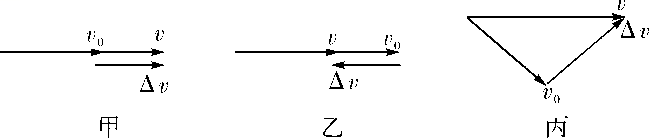
\includegraphics[width=2.94792in,height=0.625in]{media/image5.png}\end{center}
8.加速度

(1)物理意义:描述物体速度\_\_变化快慢和变化方向\_\_的物理量,是状态量.

(2)定义式:$a=\dfrac{\Delta v}{\Delta t}=\dfrac{v-v_{0}}{\Delta t}$.

(3)决定因素:a不是由$v, \Delta t, \Delta v$来决定,而是由F、M来决定.

(4)方向:与$\Delta v$的方向一致,由\_\_合外力\_\_的方向决定,而与$v_{0},v$的方向无关.

\newpage
\subsection{对质点概念的理解}
{[}例1{]}在研究下述运动时,能把物体看做质点的是( B )

A.研究短跑运动员的起跑动作时

B.研究一架无人机的飞行快慢时

C.将一枚硬币用力上抛并猜测它落地时正面是朝上还是朝下时

D.研究汽车在上坡时有无翻倒的危险时
\begin{solution}
	研究短跑运动员的起跑动作、抛出硬币落地时的上下面时,所研究对象的大小和形状不能忽略,故运动员和硬币都不能看做质点;研究汽车翻倒是转动问题,不能将汽车看做质点;研究飞机飞行快慢时,可把飞机看做质点.故选项B正确.
	
	{[}审题突破{]}明确在所研究的问题中,物体的大小和形状是主要因素还是次要因素.
\end{solution}



\begin{center}
\includegraphics[width=0.70833in,height=0.125in]{media/image13.png}

\textbf{建立质点模型的两个关键点}
\end{center}


(1)明确题目中要研究的问题是什么.质点是对实际物体的科学抽象,是研究物体运动时对实际物体进行的近似,真正的质点并不存在.

(2)分析物体的大小和形状对所研究的问题产生的影响能否忽略不计.当物体的大小和形状对所研究运动的影响很小,可以忽略不计时,就可将其视为质点.



\subsection{位移与路程的区别和联系}
\begin{longtable}[]{@{}lll@{}}
\toprule
比较项目 & 位移$x$ & 路程$l$\tabularnewline
\midrule
\endhead
决定因素 & 由始、末位置决定 & 由实际的运动轨迹长度决定\tabularnewline
运算规则 & 矢量的三角形定则或平行四边形定则 &
标量的代数运算\tabularnewline
大小关系 & $x\le l$(路程是位移被无限分割后,所分的各小段位移的绝对值的和)
&\tabularnewline
\bottomrule
\end{longtable}

{[}例2{]}(2017·湖南株洲质检)(多选)关于位移和路程,下列说法正确的是( BD )

A.物体在某一段时间内运动的位移为零,则其一定是静止的

B.物体在某一段时间内运动的路程为零,则其一定是静止的

C.在直线运动中,物体的位移大小一定等于其路程

D.在曲线运动中,物体的位移大小一定小于路程

解析 路程指物体运动轨迹的长度,而位移指由初位置指向末位置的有向线段,只有当物体做单向直线运动时,其位移大小才等于路程.容易判断选项B、D正确,A、C错误.

\newpage
\subsection{平均速度与瞬时速度的区别和联系}

1.两种物体的速度

(1)瞬时速度是运动时间$\Delta t\rightarrow 0$时的平均速度.

(2)对于匀速直线运动,瞬时速度与平均速度相等.

2.关于用平均速度法求瞬时速度

(1)方法概述:由平均速度公式$\bar v=\dfrac{\Delta x}{\Delta t}$可知,当$\Delta x$、$\Delta t$都非常小,趋向于极限时,这时的平均速度就可认为是某一时刻或某一位置的瞬时速度.

(2)选用思路:当已知物体在微小时间$\Delta t$内发生的微小位移$\Delta x$时,可由$\bar v=\dfrac{\Delta x}{\Delta t}$粗略地求出物体在该位置的瞬时速度.

{[}例3{]}(多选)如图所示,物体沿曲线轨迹的箭头方向运动,AB、ABC、ABCD、ABCDE四段曲线轨迹运动所用的时间分别是1
s、2 s、3 s、4 s.下列说法正确的是( ABC )

\begin{center}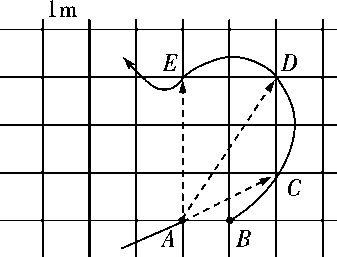
\includegraphics[width=1.53125in,height=1.16667in]{media/image14.png}\end{center}

A.物体在AB段的平均速度大小为1 m/s

B.物体在ABC段的平均速度大小为$\dfrac{\sqrt{5}}{2}$m/s

C.AB段的平均速度比ABC段的平均速度更能反映物体处于A点时的瞬时速度

D.物体在B点的速度等于AC段的平均速度

\begin{solution}
	由$\bar v=\dfrac{\Delta x}{\Delta t}$可得,$\bar v_{AB}=\dfrac{1}{1}m/s=1m/s$,$\bar v_{AC}=\dfrac{\sqrt{5}}{2}m/s$,故选项A、B均正确;所选取的过程离A点越近,其阶段的平均速度越接近A点的瞬时速度,故选项C正确;由A经B到C的过程不是匀变速直线运动过程,故B点虽为AC段的中间时刻,但其速度不等于AC段的平均速度,故选项D错误.
\end{solution}


\begin{center}
\includegraphics[width=0.70833in,height=0.125in]{media/image13.png}

\textbf{平均速度和瞬时速度的三点注意}
\end{center}

(1)求解平均速度必须明确是哪一段位移或哪一段时间内的平均速度.

(2)$\bar v=\dfrac{\Delta x}{\Delta t}$是平均速度的定义式,适用于所有的运动.

(3)用平均速度法近似求解瞬时速度,不仅适用于直线运动,也适用于曲线运动.时间越短,平均速度越接近于瞬时速度.

\newpage
\subsection{速度、速度的变化量和加速度的关系}

1.速度的大小与加速度的大小没有必然联系.

2.速度变化量与加速度没有必然的联系,速度变化量的大小由加速度和速度变化的时间决定.

3.$a=\dfrac{\Delta v}{\Delta t}$是加速度的定义式;加速度的决定式是$a=\dfrac{F}{m}$,即加速度的大小由物体受到的合力F和物体的质量m共同决定,加速度的方向由合力的方向决定.

4.速度增大或减小由速度与加速度的方向关系决定

\begin{center}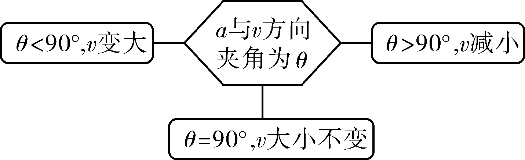
\includegraphics[width=2.38542in,height=0.72917in]{media/image15.png}\end{center}

{[}例4{]}一质点在x轴上运动,初速度$v_0$\textgreater0,加速度a\textgreater0,当加速度a的值由零逐渐增大到某一值后再逐渐减小到零,则该质点( B )

A.速度先增大后减小,直到加速度等于零为止

B.速度一直在增大,直到加速度等于零为止

C.位移先增大,后减小,直到加速度等于零为止

D.位移一直在增大,直到加速度为0为止

\begin{solution}
	由于加速度的方向始终与速度方向相同,质点速度逐渐增大,当加速度减小到零时,速度达到最大值,选项A错误,B正确;位移逐渐增大,当加速度减小到零时,速度不再变化,位移将随时间继续增大,选项C、D错误.
\end{solution}


\begin{center}
\includegraphics[width=0.70833in,height=0.125in]{media/image13.png}

\textbf{对加速度大小和方向的进一步理解}
\end{center}


\begin{center}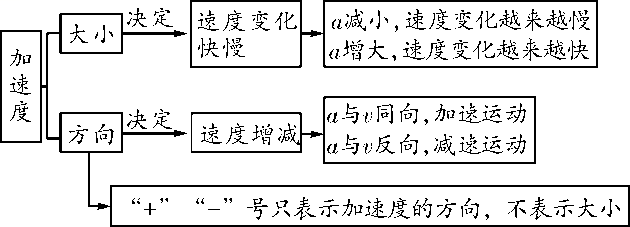
\includegraphics[width=2.86458in,height=1.03125in]{media/image16.png}\end{center}

\newpage
\section{匀变速直线运动的规律及应用}



1.基本规律

(1)速度公式:$v=v_{0}+a t$.

(2)位移公式:$x=v_{0} t+\dfrac{1}{2} a t^2$.

(3)位移速度关系式:$v^{2}-v_{0}^{2}=2 a x$.

这三个基本公式,是解决匀变速直线运动的基石.均为矢量式,应用时应规定正方向.

2.两个重要推论

(1)物体在一段时间内的平均速度等于这段时间中间时刻的瞬时速度,还等于初、末时刻速度矢量和的一半,即$v_{\dfrac{t}{2}}=\dfrac{v_{0}+v}{2}$.

(2)任意两个连续相等的时间间隔T内的位移之差为一恒量,即

$\Delta x=x_{2}-x_{1}=x_{3}-x_{2}=\ldots=x_{n}-x_{n-1}=a T^{2}$.

3.v0=0的四个重要推论

(1)1T末、2T末、3T末\ldots\ldots 瞬时速度的比为

$v_{1} : v_{2} : v_{3} : \ldots : v_{n}=1 : 2 : 3 : \ldots : n$.

(2)1T内、2T内、3T内\ldots\ldots 位移的比为

$x_{1} : x_{2} : x_{3} : \ldots : x_{0}=1^{2} : 2^{2} : 3^{2} : \ldots : n^{2}$.

(3)第一个T内、第二个T内、第三个T内\ldots\ldots 位移的比为

$x_{\mathrm{I}} : x_{\mathrm{II}} : x_{\mathrm{III}} : \ldots : x_{n}=1 : 3 : 5 : \ldots :(2 n-1)$.

(4)从静止开始通过连续相等的位移所用时间的比为

$t_{1} : t_{2} : t_{3} : \ldots : t_{n}=1 :(\sqrt{2}-1) :(\sqrt{3}-\sqrt{2}) : \ldots :(\sqrt{n}-\sqrt{n-1})$.

4.自由落体运动

(1)条件:物体只受\_\_重力\_\_,从\_\_静止\_\_开始下落.

(2)基本规律:

\ding{172}速度公式$v=g t$;

\ding{173}位移公式$h=\dfrac{1}{2} g t^{2}$;

\ding{174}速度位移关系式$v^{2}=2 g h$.

5.竖直上抛运动

(1)运动特点:加速度为g,上升阶段做\_\_匀减速直线\_\_运动,下降阶段做\_\_自由落体\_\_运动.

(2)基本规律:

\ding{172}速度公式$v=v_{0}-g t$;

\ding{173}位移公式$h=v_{0} t-\dfrac{1}{2} g t^{2}$;

\ding{174}速度位移关系式$v^{2}-v_{0}^{2}=-2 g h$.
\newpage
\subsection{匀变速直线运动的规律及应用}

1.运动学公式中正、负号的规定

(1)除时间t外,x、$\mathrm v_0$、v、a均为矢量,所以需要确定正方向,一般以$\mathrm v_0$的方向为正方向.与初速度同向的物理量取正值,反向的物理量取负值,当$\mathrm v_0$=0时,一般以加速度a的方向为正方向.

(2)五个物理量t、$\mathrm v_0$、v、a、x必须针对同一过程.

2.解决匀变速直线运动问题常用的``六法''

\begin{center}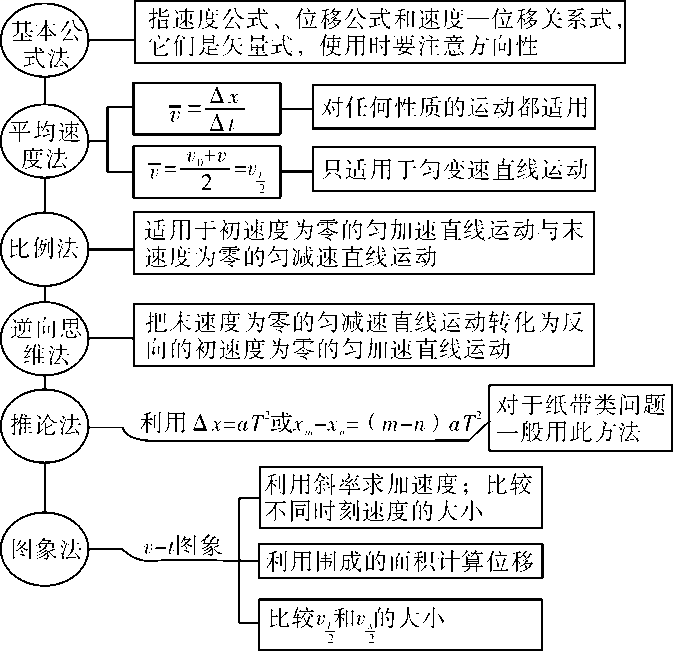
\includegraphics[width=3.06458in,height=2.96319in]{media/image23.png}\end{center}

{[}例1{]}(2017·湖南岳阳检测)如图所示,是冰壶以速度v垂直进入四个宽为l的矩形区域沿虚线做匀减速直线运动,且刚要离开第四个矩形区域的E点时速度恰好为零,冰壶通过前三个矩形的时间为t,试通过所学知识分析并计算冰壶通过第四个矩形所用的时间是多少?(可选用多种方法)

\begin{center}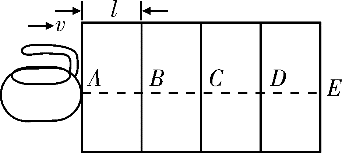
\includegraphics[width=1.55556in,height=0.69444in]{media/image24.png}\end{center}

\begin{solution}
	答案  t
\end{solution}
\begin{center}
\includegraphics[width=0.71319in,height=0.12986in]{media/image25.png}

\textbf{求解匀变速直线运动问题的基本思路}
\end{center}


画过程分析图$\rightarrow$ 判断运动性质$\rightarrow$ 选取正方向$\rightarrow$ 选用公式列方程$\rightarrow$ 解方程并讨论

\newpage
\subsection{自由落体和竖直上抛运动的分析}

{[}例2{]}(2017·山东济南调研)如图所示是一种较精确测量重力加速度g值的方法:将下端装有弹射装置的真空玻璃直管竖直放置,玻璃管足够长,小球竖直向上被弹出,在O点与弹簧分离,然后返回,在O点正上方选取一点P,利用仪器精确测得OP间的距离为H,从O点出发至返回O点的时间间隔为$T_1$,小球两次经过P点的时间间隔为$T_2$.求:

(1)重力加速度g;

(2)若O点距玻璃管底部的距离为$L_0$,求玻璃管最小长度.

\begin{center}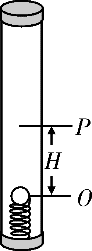
\includegraphics[width=0.41667in,height=1.13889in]{media/image26.png}\end{center}

\begin{solution}
(1)$g=\dfrac{8H}{T_1^2-T_2^2}$ (2)$L_0+\dfrac{T_1^2H}{T_1^2-T_2^2}$

(1)小球从O点上升到最高点有$h_1=\dfrac{1}{2}g(\dfrac{T_1}{2} )^2$,小球从P点上升到最高点有$h_2=\dfrac{1}{2}g(\dfrac{T_2}{2} )^2$,依据题意有$h_1-h_2=H$,联立解得$g=\dfrac{8H}{T_1^2-T_2^2}$.

(2)真空管最小长度$L=L_0+h_1$,解得$L=L_0+\dfrac{T_1^2H}{T_1^2-T_2^2}$.


\end{solution}
\begin{center}
\includegraphics[width=0.71319in,height=0.12986in]{media/image13.png}

\textbf{竖直上抛运动的分析方法}
\end{center}


(1)分段法:可以把竖直上抛运动分成上升阶段的匀减速运动和下降阶段的自由落体运动处理,下降过程是上升过程的逆过程.

(2)整体法:从全过程来看,加速度方向始终与初速度的方向相反,所以也把竖直上抛运动看成是一个匀变速直线运动.
\newpage
\section{运动图象 追及和相遇问题}



1.直线运动的x-t图象

\begin{center}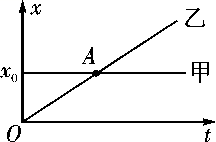
\includegraphics[width=0.97917in,height=0.64583in]{media/image29.png}\end{center}

(1)意义:反映了直线运动的物体\_\_位移\_\_随\_\_时间\_\_变化的规律.

(2)图线上某点切线的斜率的意义

\ding{172}斜率大小:表示物体速度的\_\_大小\_\_.

\ding{173}斜率的正负:表示物体速度的\_\_方向\_\_.

(3)两种特殊的x-t图象

\ding{172}若x-t图象是一条平行于时间轴的直线,说明物体处于\_\_静止\_\_状态.(如图所示甲图线)

\ding{173}若x-t图象是一条倾斜的直线,说明物体在做\_\_匀速直线\_\_运动.(如图所示乙图线)

2.直线运动的v-t图象

\begin{center}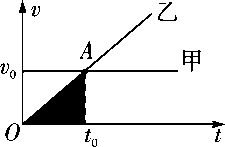
\includegraphics[width=1.02083in,height=0.66667in]{media/image30.png}\end{center}
	

(1)意义:反映了直线运动的物体\_\_速度\_\_随\_\_时间\_\_变化的规律.

(2)图线上某点切线的斜率的意义

\ding{172}斜率的大小:表示物体\_\_加速度\_\_的大小.

\ding{173}斜率的正负:表示物体\_\_加速度\_\_的方向.

(3)两种特殊的v-t图象

\ding{172}匀速直线运动的v-t图象是与横轴\_\_平行\_\_的直线.(如图所示甲图线)

\ding{173}匀变速直线运动的v-t图象是一条\_\_倾斜\_\_的直线.(如图所示乙图线)

(4)图线与坐标轴围成的``面积''的意义

\ding{172}图线与坐标轴围成的``面积''表示相应时间内的\_\_位移\_\_.

\ding{173}若此面积在时间轴的上方,表示这段时间内的位移方向为\_\_正方向\_\_;若此面积在时间轴的下方,表示这段时间内的位移方向为\_\_负方向\_\_.

3.追及和相遇问题

(1)两类追及问题

\ding{172}若后者能追上前者,追上时,两者处于\_\_同一位置\_\_,且后者速度一定不小于前者速度.

\ding{173}若追不上前者,则当后者速度与前者\_\_相等\_\_时,两者相距最近.

(2)两类相遇问题

\ding{172}同向运动的两物体追及,追上时即相遇.

\ding{173}相向运动的物体,当各自发生的位移大小之和等于开始时两物体间的距离时即相遇.

\newpage
\subsection{x-t图象与v-t图象的区别}

\begin{longtable}[]{@{}m{1.5cm}m{6cm}m{6cm}@{}}
\toprule
& x-t图象 & v-t图象\tabularnewline
\midrule
\endhead
轴 & 横轴为时间t,纵轴为位移x & 横轴为时间t,纵轴为速度v\tabularnewline
线 & 倾斜直线表示匀速直线运动 &
倾斜直线表示匀变速直线运动\tabularnewline
斜率 & 表示速度 & 表示加速度\tabularnewline
面积 & 无实际意义 & 图线和时间轴围成的面积表示位移\tabularnewline
纵截距 & 表示初位置 & 表示初速度\tabularnewline
特殊点 & 拐点表示从一种运动变为另一种运动,交点表示相遇 &
拐点表示从一种运动变为另一种运动,交点表示速度相等\tabularnewline
\bottomrule
\end{longtable}

{[}例1{]}(2018·陕西汉中期末)在平直的公路上行驶的a车和b车,其位移——时间图象分别为图中直线a和曲线b,已知b车的加速度恒定且
$ab=-2m/s^2$,当t=3 s时,直线a和曲线b刚好相切,求t=0 s时a车和b车的距离$x_0$.

\begin{center}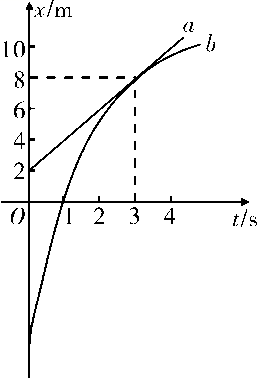
\includegraphics[width=1.16667in,height=1.71875in]{media/image33.png}\end{center}

\begin{solution}
	9 m
\end{solution}
\begin{center}
\includegraphics[width=0.70833in,height=0.125in]{media/image34.png}

\textbf{运动图象中的易错点}
\end{center}


(1)对x-t图象,图线在纵轴上的截距表示t=0时物体的位置,对v-t或a-t图象,图线在纵轴上的截距并不表示t=0时物体的位置.

(2)在v-t图象中,两条图线的交点不表示两物体相遇,而是表示两者速度相同.

(3)两条图线在v轴上的截距不同,不少同学误认为两物体的初始位置不同,位置是否相同应根据题中条件确定.
\newpage
\subsection{追及、相遇问题}

讨论追及、相遇的问题,其实质就是分析讨论两物体在同一时刻能否到达相同的空间位置问题.

1.抓住一个条件,两个关系

(1)一个条件:即两者速度相等,它往往是物体间能否追上、追不上或(两者)距离最大、最小的临界条件,也是分析判断的切入点.

(2)两个关系:即时间关系和位移关系,这两个关系可通过画运动示意图得到.

2.能否追上的判断方法

常见情形:物体A追物体B,开始二者相距$x_0$,则

(1)A追上B时,必有$x_A-x_B=x_0$,且$v_A\ge v_B$.

\begin{center}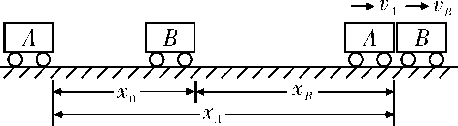
\includegraphics[width=2.08333in,height=0.57292in]{media/image35.png}\end{center}

(2)要使两物体恰好不相撞,必有$x_A-x_B=x_0$,$v_A=v_B$.

{[}例2{]}(2018·江苏镇江模拟)甲、乙两车在同一直线轨道上同向行驶,甲车在前,速度为$v_1=8m/s$,乙车在后,速度为$v_2=16 m/s$,当两车相距$x_0=8m$时,甲车因故开始刹车,加速度大小为$a_1=2m/s^2$,为避免相撞,乙车立即开始刹车,则乙车的加速度至少为多大?
\begin{solution}
	$6m/s^2$
\end{solution}


\begin{center}
\includegraphics[width=0.70833in,height=0.125in]{media/image13.png}

\textbf{追及和相遇问题的求解方法}
\end{center}


(1)解题思路

分析物体运动过程$\rightarrow$画运动示意图$\rightarrow$找两物体位移,时间,速度关系$\rightarrow$ 列位移和速度,时间方程

(2)解题技巧

\ding{172}紧抓``一图三式'',即:过程示意图,时间关系式、速度关系式和位移关系式.

\ding{173}审题应抓住题目中的关键字眼,充分挖掘题目中的隐含条件.如``刚好''\,``恰好''\,``最多''\,``至少''等.往往对应一个临界状态,满足相应的临界条件.

\ding{174}若被追赶的物体做匀减速运动,一定要注意追上前该物体是否已经停止运动,另外还要注意最后对解的讨论分析.
\newpage

\chapter{相互作用}

\section{重力 弹力 摩擦力}


1.重力

(1)产生:由于\_\_地球\_\_的吸引而使物体受到的力.

(2)大小:与物体的质量成\_\_正比\_\_,即$G=m g$.可用\_\_弹簧测力计\_\_测量重力.

(3)方向:总是\_\_竖直向下\_\_的.

(4)重心:其位置与物体的\_\_质量\_\_分布和\_\_形状\_\_有关.

2.弹力

(1)定义:发生\_\_弹性形变\_\_的物体由于要恢复原状而对与它接触的物体产生的作用力.

(2)产生的条件

\ding{172}物体间直接\_\_接触\_\_;\ding{173}接触处发生\_\_弹性形变\_\_.

(3)方向:总是与物体形变的方向\_\_相反\_\_.

3.胡克定律

(1)内容:在\_\_弹性限度\_\_内,弹力的大小跟弹簧伸长(或缩短)的长度x成\_\_正比\_\_.

(2)表达式:$F=kx$.$k$是弹簧的\_\_劲度系数\_\_,由弹簧自身的性质决定,单位是\_\_牛顿每米\_\_,用符号$\mathrm{N} / \mathrm{m}$表示.x是弹簧长度的\_\_变化量\_\_,不是弹簧形变以后的长度.

4.滑动摩擦力和静摩擦力的对比

\begin{longtable}[]{@{}m{2cm}m{6.5cm}m{6.5cm}@{}}
\toprule
名称项目& \begin{minipage}[b]{0.30\columnwidth}\raggedright
静摩擦力\strut
\end{minipage} & \begin{minipage}[b]{0.30\columnwidth}\raggedright
滑动摩擦力\strut
\end{minipage}\tabularnewline
\midrule
\endhead
定义 & 两相对静止的物体间的摩擦力 &
两相对运动的物体间的摩擦力\tabularnewline
\begin{minipage}[t]{0.30\columnwidth}\raggedright
产生条件\strut
\end{minipage} & \begin{minipage}[t]{0.30\columnwidth}\raggedright
\ding{172}接触面粗糙

\ding{173}接触处有压力

\ding{174}两物体间有相对运动趋势\strut
\end{minipage} & \begin{minipage}[t]{0.30\columnwidth}\raggedright
\ding{172}接触面粗糙

\ding{173}接触处有压力

\ding{174}两物体间有相对运动\strut
\end{minipage}\tabularnewline
\begin{minipage}[t]{0.30\columnwidth}\raggedright
大小、方向\strut
\end{minipage} & \begin{minipage}[t]{0.30\columnwidth}\raggedright
大小:$0<F_f\le F_{fmax}$

方向:与受力物体相对运动趋势的方向相反\strut
\end{minipage} & \begin{minipage}[t]{0.30\columnwidth}\raggedright
大小:$F_f=\mu F_N$

方向:与受力物体相对运动的方向相反\strut
\end{minipage}\tabularnewline
作用效果 & 总是阻碍物体间的相对运动趋势 &
总是阻碍物体间的相对运动\tabularnewline
\bottomrule
\end{longtable}

滑动摩擦力大小的计算公式$F_{\mathrm{f}}=\mu F_{\mathrm{N}}$中$\mu$为比例常数,称为动摩擦因数,其大小与两个物体的材料和接触面的粗糙程度有关.
\newpage
\subsection{弹力有无的判断}

\begin{longtable}[]{@{}m{0.2cm}m{6.1cm}m{2cm}m{5cm}@{}}
\toprule

方法& 概念& 图示&说明 \tabularnewline
\midrule
假
设
法& 假设将与研究对象接触的物体解除接触,判断研究对象的运动状态是否发生改变,若运动状态不变,则此处不存在弹力,若运动状态改变,则此处一定存在弹力  &
\begin{center}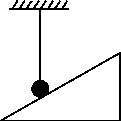
\includegraphics[width=0.55208in,height=0.55208in]{media/image40.png}\end{center}&
图中细线竖直、斜面光滑,因去掉斜面体,小球的状态不变,故小球只受细线的拉力,不受斜面的支持力\tabularnewline

替
换
法 & 用细绳替换装置中的杆件,看能不能维持原来的力学状态,如果能维持,则说明这个杆提供的是拉力;否则,提供的是支持力&
\begin{center}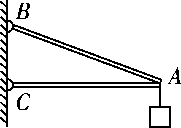
\includegraphics[width=0.82292in,height=0.58333in]{media/image41.png}\end{center}&
图中轻杆AB、AC,用绳替换AB,原装置状态不变,说明AB对A施加的是拉力;用绳替换AC,原状态不能维持,说明AC对A施加的是支持力\strut
\tabularnewline
状
态
法 & 由运动状态分析弹力,即物体的受力必须与物体的运动状态相符合,依据物体的运动状态,由二力平衡(或牛顿第二定律)列方程,求解物体间的弹力 &
\begin{center}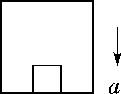
\includegraphics[width=0.55208in,height=0.42708in]{media/image42.png}\end{center}&
升降机以a=g加速下降时物体不受底板的弹力作用\tabularnewline
\bottomrule
\end{longtable}

{[}例1{]}(2017·陕西西安调研)如图所示,在一个正方体的盒子中放有一个质量分布均匀的小球,小球的直径恰好和盒子内表面正方体的棱长相等,盒子沿倾角为$\alpha$的固定斜面滑动,不计一切摩擦,下列说法中正确的是( A )

\begin{center}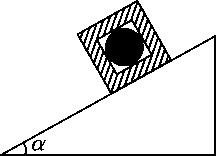
\includegraphics[width=0.97917in,height=0.70833in]{media/image43.png}\end{center}

A.无论盒子沿斜面上滑还是下滑,球都仅对盒子的下底面有压力

B.盒子沿斜面下滑时,球对盒子的下底面和右侧面有压力

C.盒子沿斜面下滑时,球对盒子的下底面和左侧面有压力

D.盒子沿斜面上滑时,球对盒子的下底面和左侧面有压力

{[}思维导引{]}采用假设法,可假设小球仅对盒子的下底有压力,判断两者运动是否相同.
\begin{solution}
	先以盒子和小球组成的系统为研究对象,无论上滑还是下滑,用牛顿第二定律均可求得系统的加速度大小为a=gsin
$\alpha$,方向沿斜面向下,由于盒子和小球始终保持相对静止,所以小球的加速度大小也是a=gsin
$\alpha$,方向沿斜面向下,小球沿斜面向下的重力分力大小恰好等于所需的合外力,因此不需要盒子的左、右侧面提供弹力.故选项A正确.
\end{solution}

\begin{center}
\includegraphics[width=0.70833in,height=0.125in]{media/image44.png}\end{center}
对于形变明显的物体,由形变情况直接判断弹力情况,对于形变不明显的物体通常用``假设法''和``替换法'',有时要根据物体的运动状态判定弹力情况.

\subsection{弹力方向的确定和大小的计算}

1.弹力方向的确定

\begin{center}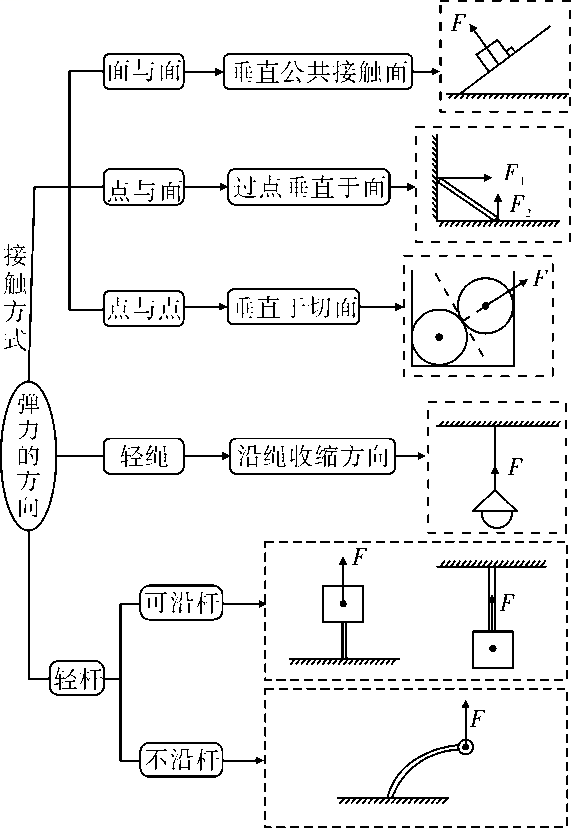
\includegraphics[width=2in]{media/image45.png}\end{center}
2.计算弹力大小的三种方法

(1)根据胡克定律进行求解.(2)根据力的平衡条件进行求解.(3)根据牛顿第二定律进行求解.

{[}例2{]}如图所示,固定在小车支架上的斜杆与竖直杆的夹角为$\theta$,在斜杆下端固定一个质量为m的小球,下列关于杆对球的作用力F的判断中正确的是( D )\begin{center}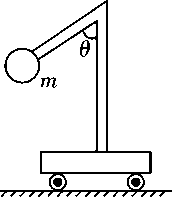
\includegraphics[width=0.78125in,height=0.89583in]{media/image46.png}\end{center}

A.小车静止时,$F=mg\cos \theta$,方向沿杆向上

B.小车静止时,$F=mg\cos \theta$,方向垂直杆向上

C.小车向右以加速度a运动时,一定有$F=\dfrac{mg}{\sin\theta}$

D.小车向左以加速度a运动时,$F=\sqrt{(ma)^2+(mg)^2}$,方向斜向左上方,与竖直方向的夹角为$\alpha$满足$tan\alpha=\dfrac{a}{g}$

{[}例3{]}缓冲装置可抽象成如图所示的简单模型,图中A、B为原长相等、劲度系数分别为$k_1$、$k_2$($k_1\neq k_2$)的两个不同的轻质弹簧.下列表述正确的是( D )

\begin{center}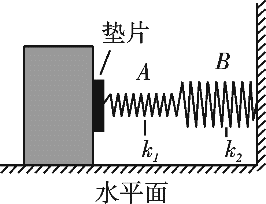
\includegraphics[width=1.20833in,height=0.92708in]{media/image47.png}\end{center}

A.装置的缓冲效果与两弹簧的劲度系数无关

B.垫片向右移动稳定后,两弹簧产生的弹力之比$F_1:F_2=k_1:k_2 $

C.垫片向右移动稳定后,两弹簧的长度之比$l_1:l_2=k_2:k_1$

D.垫片向右移动稳定后,两弹簧的压缩量之比$x_1:x_2=k_2:k_1$ 

{[}思维导引{]}\ding{172}分析稳定后,两弹簧之间相互弹力作用的关系.\ding{173}利用胡克定律计算两个弹簧的形变量和长度.

\subsection{静摩擦力的大小和方向}

1.静摩擦力有无的判断

(1)假设法

静摩擦力的方向一定与物体相对运动趋势的方向相反,利用``假设法''可以判断出物体相对运动趋势的方向.

假设法(如图所示)

\begin{center}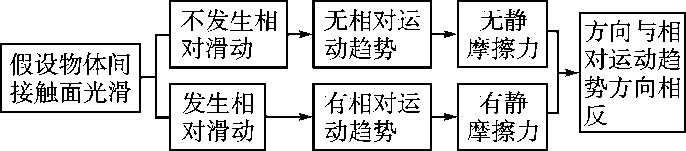
\includegraphics[width=3.11458in,height=0.6875in]{media/image48.png}\end{center}

(2)状态法

此法关键是先判明物体的运动状态(即加速度的方向),再利用牛顿第二定律(F=ma)确定合力,然后通过受力分析确定静摩擦力的大小及方向.

(3)牛顿第三定律法

此法的关键是抓住``力是物体间的相互作用'',先确定受力较少的物体受到的静摩擦力的方向,再根据``力的相互性''确定另一物体受到的静摩擦力方向.

2.静摩擦力的计算方法

(1)最大静摩擦力$F_{fmax}$的计算

最大静摩擦力$F_{fmax}$只在刚好要发生相对滑动这一特定状态下才表现出来.比滑动摩擦力稍大些,通常认为二者相等,即$F_{fmax}=\mu F_N$. 

(2)一般静摩擦力的计算

一般静摩擦力F的大小和方向都与产生相对运动趋势的力密切相关,跟接触面间相互挤压的弹力$F_N$无直接关系,因此具有大小、方向的可变性.对具体问题要结合研究对象的运动状态(静止、匀速运动或加速运动),利用平衡条件或牛顿运动定律列方程求解.



\begin{center}
\includegraphics[width=0.70833in,height=0.125in]{media/image34.png}

\textbf{应用``状态法''解题时应注意的问题}
\end{center}


状态法是分析判断静摩擦力有无及方向、大小的常用方法,在使用状态法处理问题时,需注意以下两点:

(1)明确物体的运动状态,分析物体的受力情况,根据平衡方程或牛顿定律求解静摩擦力的大小和方向.

(2)静摩擦力的方向与物体的运动方向没有必然关系,可能相同,也可能相反,还可能成一定的夹角.
\newpage
\subsection{滑动摩擦力的大小和方向}

1.产生的条件

(1)两物体相互接触且挤压,发生形变,产生弹力.

(2)两接触面粗糙.

(3)两物体沿接触面发生相对运动.

以上三个条件必须同时具备,才会有滑动摩擦力存在.

2.在计算滑动摩擦力的公式$F_f=\mu F_N$中,$\mu$为动摩擦因数,其大小与接触面的材料、表面的粗糙程度有关;$F_N$为两接触面间的正压力,其大小不一定等于物体的重力.

3.滑动摩擦力的大小与物体的运动速度无关,与接触面积也无关.

4.滑动摩擦力的方向总是与物体间相对运动的方向相反,但不一定与物体运动方向相反.

{[}例5{]}(2017·吉林长春检测)如图所示,质量为m的工件置于水平放置的钢板C上,二者间动摩擦因数为$\mu$,由于固定的光滑导槽A、B的控制,工件只能沿水平导槽运动,现使钢板以速度$v_1$向右运动,同时用F拉动工件(F方向与导槽平行)使其以速度$v_2$沿导槽运动,则F的大小为( C )

\begin{center}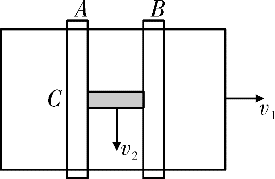
\includegraphics[width=1.25in,height=0.8125in]{media/image50.png}\end{center}

A.等于$\mu mg$ B.大于$\mu mg$

C.小于$\mu mg$ D.不能确定
\begin{solution}
	钢板以速度$v_1$向右运动,则工件以等大速度相对钢板向左移动,设为$v_1^{'}$,同时工件被拉动也具有另一速度$v_2$,故工件相对于钢板的运动速度应是$v_1^{'}$与$v_2$的合成,即如上图中的速度v.滑动摩擦力阻碍二者的相对运动,故工件所受摩擦力$F_f$与v方向相反,要使工件沿导槽匀速运动,所施加的拉力只需与$F_f$一个分力平衡,故 $F< F_f=\mu mg$.
\end{solution}

\begin{center}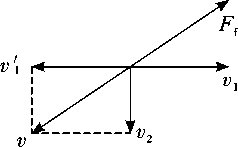
\includegraphics[width=1.08333in,height=0.66667in]{media/image51.png}\end{center}
\newpage
\subsection{摩擦力突变问题}

\begin{center}
\includegraphics[width=0.70833in,height=0.125in]{media/image37.png}

\textbf{解决摩擦力突变问题的关键点}
\end{center}


物体受到的外力发生变化时,物体受到的摩擦力的种类就有可能发生突变.解决这类问题的关键是:正确对物体受力分析和运动状态分析,从而找到物体摩擦力的突变``临界点''.

常见类型如下:

(1)静---静``突变''

当作用在物体上的其他力的合力发生变化时,物体仍保持静止,而所受静摩擦力方向发生$180^\circ$``突变'',则``突变''点是静摩擦力为零时.

(2)动---动``突变''

某物体相对于另一物体滑动的过程中,若相对运动方向变了,则滑动摩擦力方向发生``突变'',``突变''点为两物体相对速度为零时.

(3)静---动``突变''

物体在摩擦力和其他力作用下处于静止状态,当其他力变化时,如果物体不能保持静止状态,则物体受到的静摩擦力将``突变''成滑动摩擦力,``突变''点为静摩擦力达到最大值时.

(4)动---静``突变''

两物体相对减速滑动的过程中,若相对速度变为零,则滑动摩擦力``突变''为静摩擦力,``突变''点为两物体相对速度刚好为零时.

{[}例6{]}(多选)如图所示,将两相同的木块a、b置于粗糙的水平地面上,中间用一轻弹簧连接,两侧用细绳系于墙壁.开始时a、b均静止,弹簧处于伸长状态,两细绳均有拉力,a所受摩擦力$F_{fa}\neq 0$,b所受摩擦力$F_{fb}=0$.现将右侧细绳剪断,则剪断瞬间( AD )

\begin{center}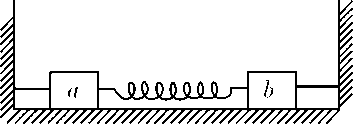
\includegraphics[width=1.60417in,height=0.5625in]{media/image52.png}\end{center}

A.$F_{fa}$大小不变 B.$F_{fa}$方向改变
C.$F_{fb}$仍然为零 D.$F_{fb}$方向向右

{[}例7{]}传送带以恒定的速率v=10m/s运动,已知它与水平面成$\alpha=37^\circ$,如图所示,PQ=16m,将一个小物体无初速度地放在P点,小物体与传送带间的动摩擦因数为$\mu=0.5$,问当传送带逆时针转动时,小物体运动到Q点的时间为多少?($cos37^\circ=0.8,sin 37^\circ=0.6$,g取$10 m/s^2$)

\begin{center}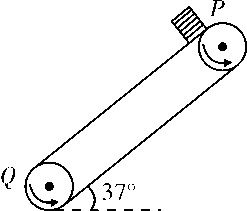
\includegraphics[width=1.125in,height=0.95833in]{media/image53.png}\end{center}

\begin{solution}
	2 s
\end{solution}
\begin{center}
\includegraphics[width=0.70833in,height=0.125in]{media/image25.png}

\textbf{摩擦力突变问题的分析步骤}
\end{center}


\begin{center}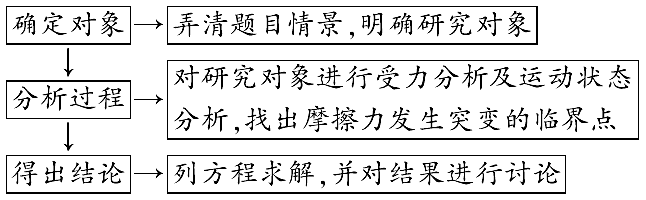
\includegraphics[width=2.8125in,height=0.875in]{media/image54.png}\end{center}
\newpage
\section{力的合成与分解}


1.力的合成

(1)合力与分力

\ding{172}定义:如果几个力共同作用产生的效果与一个力的作用效果相同,这一个力就叫做那几个力的\_\_合力\_\_,那几个力叫做这一个力的\_\_分力\_\_.

\ding{173}关系:合力与分力是\_\_等效替代\_\_关系.

(2)共点力

作用在物体的\_\_同一点\_\_,或作用线的\_\_延长线\_\_交于一点的几个力.

\begin{center}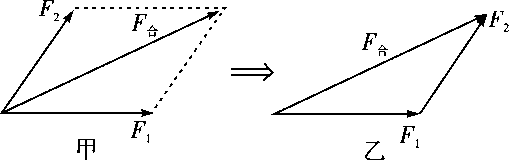
\includegraphics[width=2.3125in,height=0.72917in]{media/image61.png}
	
\end{center}
(3)力的合成

\ding{172}定义:求几个力的\_\_合力\_\_的过程.

\ding{173}运算法则

平行四边形定则:求两个互成角度的\_\_共点力\_\_的合力,可以用表示这两个力的线段为邻边作平行四边形,这两个邻边之间的对角线就表示合力的\_\_大小\_\_和\_\_方向\_\_(图甲).

三角形定则:把两个矢量的首尾顺次连接起来,第一个矢量的首到第二个矢量的尾的\_\_有向线段\_\_为合矢量(图乙).

2.力的分解

(1)定义

求一个力的\_\_分力\_\_的过程,力的分解是\_\_力的合成\_\_的逆运算.

(2)遵循的原则

\ding{172}\_\_平行四边形\_\_定则.

\ding{173}\_\_三角形\_\_定则.

(3)分解方法

\ding{172}力的作用效果分解法.

\ding{173}正交分解法.

3.矢量和标量

(1)矢量

既有大小又有\_\_方向\_\_的物理量,相加时遵循\_\_平行四边形\_\_定则.如速度、力等.

(2)标量

只有大小没有\_\_方向\_\_的物理量,求和时按算术法则相加.如路程、动能等.
\newpage
\subsection{共点力的合成}

1.共点力合成的常用方法

(1)作图法

从力的作用点沿两个分力的作用方向按同一标度作出两个分力$F_1$、$F_2$,以这两个力为邻边作一个平行四边形,这两个力所夹对角线表示这两个力的合力.通常可分别用刻度尺和量角器直接量出合力的大小和方向.

(2)解析法

根据力的平行四边形定则作出力的合成的图示,如图所示.

\begin{center}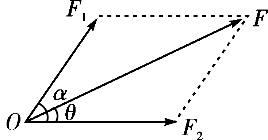
\includegraphics[width=1.21875in,height=0.63542in]{media/image64.png}\end{center}

$F=\sqrt{F_1^2+F_2^2+2F_1F_2\cos\alpha}$.

它与$F_2$的夹角为$\theta$,$\tan \theta=\dfrac{F_1\sin\alpha}{F_2+F_1\cos\alpha}$.

2.几种特殊情况的共点力的合成

\begin{longtable}[]{@{}m{4cm}m{3cm}m{3cm}@{}}
\toprule
类型 & 作图 & 合力的计算\tabularnewline
\midrule
\endhead

互相垂直& \begin{center}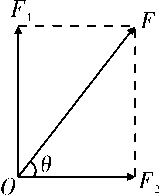
\includegraphics[width=0.5in]{media/image65.png}\end{center}&
$F=\sqrt{F_1^2+F_2^2}$

$\tan\theta=\dfrac{F_1}{F_2}$\tabularnewline

两力等大,夹角$\theta$ &
\begin{center}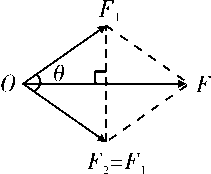
\includegraphics[width=0.7in,]{media/image66.png}\end{center}
&
$F=2F_1\cos\dfrac{\theta}{2}$

$F$与$F_1$夹角为$\dfrac{\theta}{2}$\tabularnewline
两力等大且夹角$120^\circ$ &
\begin{center}
	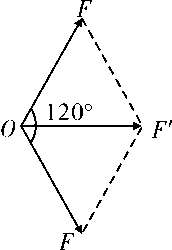
\includegraphics[width=0.6in]{media/image67.png}
\end{center}
 &
合力与分力等大\tabularnewline
\bottomrule
\end{longtable}

\begin{center}
\includegraphics[width=0.70833in,height=0.125in]{media/image34.png}

\textbf{作图法求合力的四点要求}
\end{center}


(1)分力、合力的作用点相同,切忌弄错表示合力的对角线

(2)分力、合力的比例要一致,力的标度要适当

(3)虚线、实线要分清,表示分力和合力的两条邻边和对角线画成实线,并加上箭头,平行四边形的另两条边画成虚线

(4)求合力时既要求出合力的大小,又要求出合力的方向

{[}例1{]}(2017·天津卷)(多选)如图所示,轻质不可伸长的晾衣绳两端分别固定在竖直杆M、N上的a、b两点,悬挂衣服的衣架挂钩是光滑的,挂于绳上处于静止状态.如果只人为改变一个条件,当衣架静止时,下列说法正确的是( AB )

\begin{center}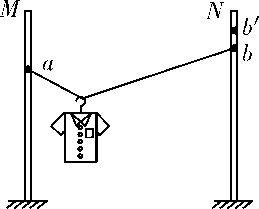
\includegraphics[width=1.17708in,height=0.94792in]{media/image68.png}\end{center}

A.绳的右端上移到$b^{'}$,绳子拉力不变

B.将杆N向右移一些,绳子拉力变大

C.绳的两端高度差越小,绳子拉力越小

D.若换挂质量更大的衣服,则衣架悬挂点右移
\begin{solution}
	oa、ob为一根绳,两端拉力相等,设绳aob长为L,M、N的水平距离为d,bo延长线交M于$a^{'}$,由几何知识知$a^{'}o=ao$,$\sin\theta=\dfrac{d}{L}$,由平衡条件有$2F\cos\theta=mg$,则$F=\dfrac{mg}{2\cos\theta^{'}}$,当b上移到$b^{'}$时,d、L不变,$\theta$不变,故F不变,选项A正确,C错误.将杆N向右移一些,L不变,d变大,$\theta$变大,$\cos\theta$变小,则F变大,选项B正确.只改变m,其他条件不变,则$\sin\theta$不变,$\theta$不变,衣架悬挂点不变,选项D错误.
\end{solution}


\begin{center}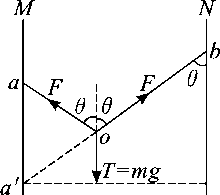
\includegraphics[width=1in,height=0.88542in]{media/image69.png}\end{center}
\begin{center}
\includegraphics[width=0.70833in,height=0.125in]{media/image13.png}\end{center}

(1)力合成时,要正确理解合力与分力的大小关系:合力与分力的大小关系要视情况而定,不能形成合力总大于分力的思维定式.

(2)合力与它的分力是等效替代关系,在进行有关力的计算时,如果已计入了合力,就不能再计入分力;如果已计入了分力,就不能再计入合力.
\newpage
\subsection{力的分解}

1.按力的作用效果分解(思路图)

\begin{center}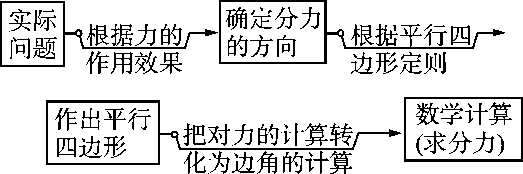
\includegraphics[width=2.375in,height=0.79167in]{media/image70.png}\end{center}

如图所示,物体的重力G按产生的效果分解为两个分力,$F_1$使物体下滑,$F_2$使物体压紧斜面.

\begin{center}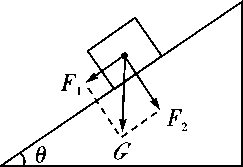
\includegraphics[width=1.10417in,height=0.76042in]{media/image71.png}\end{center}

2.正交分解法

(1)定义:将已知力按互相垂直的两个方向进行分解的方法.

(2)建立坐标轴的原则:一般选共点力的作用点为原点,在静力学中,以少分解力和容易分解力为原则(使尽量多的力在坐标轴上);在动力学中,往往以加速度方向和垂直加速度方向为坐标轴建立坐标系.

(3)方法:物体受到多个力$F_1$、$F_2$、$F_3$\ldots\ldots 作用,求合力F时,可把各力向相互垂直的x轴、y轴分解.

\begin{center}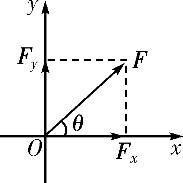
\includegraphics[width=0.83333in,height=0.83333in]{media/image72.png}\end{center}

x轴上的合力:

$F_x=F_{x1}+F_{x2}+F_{x3}+\ldots\ldots{}$

y轴上的合力:

$F_y=F_{y1}+F_{y2}+F_{y3}+\ldots\ldots{}$

合力大小:

$F=\sqrt{F_x^2+F_y^2}$

合力方向:与x轴夹角为$\theta$,则$\tan \theta=\dfrac{F_y}{F_x}$.

{[}例2{]}如图所示,光滑斜面的倾角为$\theta$,有两个相同的小球,分别用光滑挡板A、B挡住,挡板A沿竖直方向,挡板B垂直于斜面,则两挡板受到小球压力的大小之比为\_\_$1:\cos\theta$\_\_,斜面受到两个小球压力大小之比为\_\_$1:\cos^2\theta$\_\_.

\begin{center}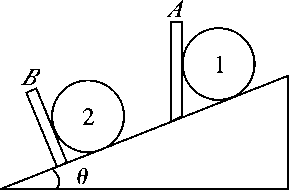
\includegraphics[width=1.3125in,height=0.86458in]{media/image73.png}\end{center}

{[}思维导引{]}既然求解的是挡板和斜面实际受到的压力,就应按力的作用效果分解力.

\subsection{``绳------杆''模型}

1.``死结''与``活结''模型

(1)``死结''可理解为把绳子分成两段,且不可以沿绳子移动的结点.``死结''两侧的绳因结而变成了两根独立的绳.

(2)``活结''可理解为把绳子分成两段,且可以沿绳子移动的结点.``活结''一般是由绳跨过滑轮或者绳上挂一光滑挂钩而形成的.实质还是同一根绳子.

2.``固定杆''与``活动杆''模型

(1)一般情况下,插入墙中的杆属于固定杆(如钉子).

(2)一端用铰链相连的杆属于活动杆.

\begin{center}
\includegraphics[width=0.70833in,height=0.125in]{media/image37.png}

\textbf{``绳------杆''模型的处理方法}
\end{center}


(1)无论``死结''还是``活结''一般均以结点为研究对象进行受力分析.

(2)由``死结''分开的两段绳子上的弹力不一定相等;由``活结''分开的两段绳子上弹力的大小一定相等,两段绳子合力的方向一定沿这两段绳子夹角的平分线.

(3)固定杆的弹力方向不一定沿杆的方向,而活动杆的弹力方向一定沿杆的方向.

{[}例3{]}如图甲所示,细绳AD跨过固定的水平轻杆BC右端的定滑轮挂住一个质量为$M_1$的物体,$\angle ACB=30^\circ$;图乙中轻杆HG一端用铰链固定在竖直墙上,另一端G通过细绳EG拉住,EG与水平方向也成$30^\circ$,轻杆的G点用细绳GF拉住一个质量为$M_2$的物体.求:

\begin{center}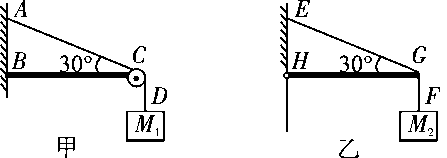
\includegraphics[width=2.03125in,height=0.71875in]{media/image74.png}\end{center}

(1)细绳AC段的张力$F_{AC}$与细绳EG的张力$F_{EG}$之比;

(2)轻杆BC对C端的支持力;

(3)轻杆HG对G端的支持力.

{[}思维导引{]}(1)判断杆的作用力方向是否沿杆方向.(2)选取恰当的研究对象.
\begin{solution}

	(1)$\dfrac{M_1}{2M_2}$ 
	
	(2)$M_1g$,方向与水平方向成$30^\circ$指向右上方
	
	(3)$\sqrt{3} M_2g$,方向水平向右
\end{solution}


\newpage
\section{受力分析 共点力的平衡}


1.受力分析

(1)定义

把指定物体(研究对象)在特定的物理环境中受到的所有外力都找出来,并画出受力图,这个过程就是受力分析.

(2)受力分析的顺序

先找重力,再找接触力(弹力、摩擦力),最后分析电场力、磁场力及其他力.

(3)受力分析的步骤

\ding{172}明确研究对象------确定分析受力的物体,研究对象可以是单个物体,也可以是多个物体的组合.

\ding{173}隔离物体分析------将研究对象从周围物体中\_\_隔离\_\_出来,进而分析物体受的重力、弹力、摩擦力、电磁力等,检查周围有哪些物体对它施加了力的作用.

\ding{174}画出受力示意图------边分析边将力一一画在受力示意图上,准确标出\_\_方向\_\_.

\ding{175}检查画出的每一个力能否找出它的\_\_施力物体\_\_,检查分析结果能否使研究对象处于题目所给的运动状态,否则,必然发生了漏力、添力或错力现象.

2.共点力的平衡

(1)平衡状态:物体处于静止或\_\_匀速直线运动\_\_状态.

(2)共点力的平衡条件:$F_{\text{合}}=0$或者$\left\{\begin{array}{l}F_{x}=0 \\ F_{y}=0\end{array}\right.$

(3)平衡条件的推论.

\ding{172}二力平衡

如果物体在两个共点力的作用下处于平衡状态,这两个力必定大小\_\_相等\_\_、方向\_\_相反\_\_,为一对平衡力.

\ding{173}三力平衡

如果物体在三个共点力的作用下处于平衡状态,其中任意两个力的合力一定与第三个力大小\_\_相等\_\_、方向\_\_相反\_\_.

\ding{174}多力平衡

如果物体受多个力作用处于平衡状态,其中任何一个力与其余力的合力大小\_\_相等\_\_、方向\_\_相反\_\_.

{[}思考感悟{]}(1)物体在某一时刻速度为零时,物体不一定处于平衡状态.(2)在多个共点力作用下的物体处于静止状态,如果其中一个力消失其他力保持不变,物体沿消失的力的反方向做初速度为零的匀加速直线运动.
\newpage
\subsection{物体的受力分析}

\begin{center}\includegraphics[width=0.70833in,height=0.125in]{media/image37.png}

\textbf{整体法、隔离法在受力分析时的灵活运用.}
\end{center}


(1)当所涉及的物理问题是整体与外界作用时,应用整体分析法,可使问题简单明了,而不必考虑内力的作用.

(2)当涉及的物理问题是物体间的相互作用时,应用隔离分析法,这时系统中物体间相互作用的内力就会变为各个独立物体的外力.

{[}例1{]}(2018·浙江宁波调研)如图所示,斜面小车M静止在光滑水平面上,一边紧贴墙壁.若再在斜面上加一物体m,且M、m相对静止,小车后来受力个数为( B )

\begin{center}\includegraphics[width=0.97917in,height=0.83333in]{media/image82.png}\end{center}

A.3 

B.4

C.5 

D.6
\begin{solution}
	对M和m整体,它们必受到重力和地面支持力,因小车静止,由平衡条件知墙面对小车必无作用力.以小车为研究对象,如右图所示,它受四个力:重力Mg,地面的支持力$F_{N1}$,m对它的压力$F_{N2}$和摩擦力$F_f$.由于m静止,可知$F_f$和$F_{N2}$的合力必竖直向下,故选项B正确.
\end{solution}

\begin{center}\includegraphics[width=0.8125in,height=0.79167in]{media/image83.png}\end{center}
\newpage
\subsection{解决平衡问题常用的方法}

\begin{longtable}[]{@{}m{2.5cm}m{10.5cm}@{}}
\toprule
方法 & 内容\tabularnewline
\midrule
\endhead
分解法 &
物体受到几个力的作用,将某一个力按力的效果进行分解,则其分力和其他力在所分解的方向上满足平衡条件\tabularnewline
合成法 &
物体受几个力的作用,通过合成的方法将它们简化成两个力,这两个力满足二力平衡条件\tabularnewline
正交分解法 &
将处于平衡状态的物体所受的力分解为相互正交的两组,每一组的力都满足二力平衡条件\tabularnewline
力的三角形法 &
物体受同一平面内三个互不平行的力的作用平衡时,这三个力的矢量箭头首尾相接,构成一个矢量三角形;反之,若三个力矢量箭头首尾相接恰好构成三角形,则这三个力的合力必为零.利用三角形法,根据正弦定理、余弦定理或相似三角形等数学知识可求得未知力\tabularnewline
\bottomrule
\end{longtable}

{[}例2{]}(2018·湖南常德模拟)如图所示,重为G的均匀链条,两端用等长的轻绳连接,挂在等高的地方,轻绳与水平方向成$\theta$角.试求:

\begin{center}\includegraphics[width=1.03125in,height=0.5in]{media/image84.png}\end{center}

(1)绳子的拉力;

(2)链条在最低点的相互拉力的大小.
\begin{solution}
	(1)$\dfrac{G}{2\sin\theta}$ (2)$\dfrac{1}{2} G\cot \theta$
\end{solution}

\begin{center}\includegraphics[width=0.70833in,height=0.125in]{media/image13.png}

\textbf{应用平衡条件解题步骤}
\end{center}


(1)选取研究对象:根据题目要求,选取一个平衡体(单个物体或系统,也可以是结点)作为研究对象.

(2)画受力示意图:对研究对象进行受力分析,画出受力示意图.

(3)三个力直接合成或正交分解,四个及四个以上的力正交分解.

(4)列方程求解:根据平衡条件列出平衡方程,解平衡方程,对结果进行讨论.
\newpage
\subsection{动态平衡问题}

1.动态平衡

在某一物理过程中,物体或系统始终处于平衡状态,而物体或系统受到的力有一部分是变力(力的大小变或方向变或大小和方向均发生变化),这样的物理过程叫动态平衡.

2.基本思路

化``动''为``静'',``静''中求``动''.

3.``两种''典型方法

\begin{center}\includegraphics[width=3.39583in,height=1.80208in]{media/image85.png}\end{center}

{[}例3{]}(2017·江苏南京调研)(多选)如图所示,在粗糙水平地面上放着一个截面为四分之一圆弧的柱状物体A,A的左端紧靠竖直墙,A与竖直墙之间放一光滑圆球B,已知A的圆半径为球B的半径的3倍,球B所受的重力为G,整个装置处于静止状态.设墙壁对B的压力为$F_1$,A对B的压力为$F_2$,则若把A向右移动少许后,它们仍处于静止状态,则$F_1$、$F_2$的变化情况分别是( AD )

\begin{center}\includegraphics[width=0.92708in,height=0.73958in]{media/image86.png}\end{center}

A.$F_1$减小 

B.$F_1$增大

C.$F_2$增大 

D.$F_2$减小
\newpage
\subsection{平衡中的临界与极值问题}

1.临界问题

当某物理量变化时,会引起其他几个物理量的变化,从而使物体所处的平衡状态``恰好出现''或``恰好不出现'',在问题的描述中常用``刚好''\,``刚能''\,``恰好''等语言叙述.

2.极值问题

平衡物体的极值,一般指在力的变化过程中的最大值和最小值问题.

3.解决平衡中临界与极值问题的常用方法

(1)图解法:根据物体的平衡条件,作出力的矢量图,通过对物理过程的分析,利用平行四边形定则进行动态分析,确定最大值与最小值.

(2)数学解法:通过对问题的分析,依据物体的平衡条件写出物理量之间的函数关系(或画出函数图象),用数学方法求极值(如求二次函数极值、公式极值、三角函数极值).

{[}例4{]}(2018·云南师大附中质检)如图所示,质量为m的小球与细线连接且静止于光滑斜面上,斜面足够长,倾角$\alpha=30^\circ$的斜面体置于光滑水平面上,用水平力F推斜面体使斜面体缓慢地向左移动,小球沿斜面缓慢升高.当细线拉力最小时,推力F等于( A )

\begin{center}\includegraphics[width=1.09375in,height=0.6875in]{media/image87.png}\end{center}

A.$\dfrac{\sqrt{3}}{4} mg$ 

B.$\dfrac{\sqrt{3}}{2} mg$

C.mg 

D.$\sqrt{3} mg$
\begin{solution}
	小球受力动态平衡如图,可知当$T$平行于斜面时$T_{min}=mg\sin 30^\circ$,对小球和斜面体组成的系统,$F=T_{min}\cos 30^\circ=mg$,选项A正确.

\begin{center}\includegraphics[width=0.85417in,height=0.98958in]{media/image88.png}\end{center}
\end{solution}


\chapter{牛顿运动定律}
\section{牛顿第一、第三定律}


1.牛顿第一定律

(1)内容

一切物体总保持\_\_匀速直线运动\_\_状态或\_\_静止\_\_状态,直到有外力迫使它改变这种状态为止.

(2)意义

\ding{172}指出了一切物体具有\_\_惯性\_\_,因此牛顿第一定律又称\_\_惯性定律\_\_.

\ding{173}指出力不是\_\_维持\_\_物体运动状态的原因,而是\_\_改变\_\_物体运动状态的原因,即力是产生\_\_加速度\_\_的原因.

\ding{174}当物体不受力时,物体总保持\_\_匀速直线运动\_\_状态或\_\_静止\_\_状态.

(3)惯性

\ding{172}定义:物体具有保持原来\_\_匀速直线运动\_\_状态或\_\_静止\_\_状态的性质.

\ding{173}量度:\_\_质量\_\_是物体惯性大小的唯一量度,与物体的运动状态、受力情况、地理位置均无关,\_\_质量大\_\_的物体惯性大,\_\_质量小\_\_的物体惯性小.

\ding{174}普遍性:惯性是物体的\_\_固有\_\_属性,一切物体都有惯性.

2.牛顿第三定律

(1)作用力和反作用力

两个物体之间的作用总是\_\_相互\_\_的,一个物体对另一个物体施加了力,另一个物体同时对这个物体也施加了力.

(2)内容

两个物体之间的作用力和反作用力总是大小\_\_相等\_\_、方向\_\_相反\_\_、作用在\_\_同一条直线上\_\_.

(3)表达式

$F=-F^{\prime}$.

(4)意义

建立了相互作用物体之间的联系及作用力与\_\_反作用力\_\_的相互依赖关系.

\newpage
\subsection{牛顿第一定律的应用技巧}

1.应用牛顿第一定律分析实际问题时,要把生活感受和理论问题联系起来深刻认识力和运动的关系,正确理解力不是维持物体运动状态的原因,克服生活中一些错误的直观印象,建立正确的思维习惯.

2..如果物体的运动状态发生改变,则物体必然受到不为零的合外力作用.因此,判断物体的运动状态是否改变,以及如何改变,应分析物体的受力情况.

{[}例1{]}伽利略创造性地把实验、假设和逻辑推理相结合的科学方法,有力地促进了人类科学认识的发展,利用如图所示的装置做如下实验:小球从左侧斜面上的O点由静止释放后沿斜面向下运动,并沿右侧斜面上升.斜面上先后铺垫三种粗糙程度逐渐降低的材料时,小球沿右侧斜面上升到的最高位置依次为1、2、3.根据三次实验结果的对比,可以得到的最直接的结论是( A )

\begin{center}\includegraphics[width=0.88542in,height=0.28125in]{media/image95.png}\end{center}

A.如果斜面光滑,小球将上升到与O点等高的位置

B.如果小球不受力,它将一直保持匀速运动或静止状态

C.如果小球受到力的作用,它的运动状态将发生改变

D.小球受到的力一定时,质量越大,它的加速度越小
\begin{solution}
	根据题意,铺垫材料粗糙程度降低时,小球上升的最高位置升高,当斜面绝对光滑时,小球在斜面上没有能量损失,因此可以上升到与O点等高的位置,而B、C、D三个选项,从题目不能直接得出,所以选项A正确.
\end{solution}


\subsection{对牛顿第三定律的理解及应用}

1.相互作用力的特点:``三同、三异、三无关''.

(1)三同:同大小;同时产生、变化、消失;同性质

(2)三异:反向;异体,即作用力、反作用力作用在不同物体上;不同效果

(3)三无关:与物体的种类无关;与相互作用的两物体的运动状态无关;与是否和其他物体相互作用无关

2.一对平衡力与作用力、反作用力的不同点:

\begin{longtable}[]{@{}lll@{}}
\toprule


  & \begin{minipage}[b]{0.30\columnwidth}\raggedright
一对平衡力\strut
\end{minipage} & \begin{minipage}[b]{0.30\columnwidth}\raggedright
作用力与反作用力\strut
\end{minipage}\tabularnewline
\midrule
\endhead
作用对象 & 同一个物体 & 两个相互作用的不同物体\tabularnewline
作用时间 & 不一定同时产生、同时消失 &
一定同时产生、同时消失\tabularnewline
力的性质 & 不一定相同 & 一定相同\tabularnewline
作用效果 & 可相互抵消 & 不可抵消\tabularnewline
\bottomrule
\end{longtable}



\begin{center}\includegraphics[width=0.70833in,height=0.125in]{media/image34.png}

\textbf{应用牛顿第三定律应注意的三个问题}
\end{center}


(1)定律中的``总是''说明对于任何物体,在任何情况下牛顿第三定律都是成立的.

(2)作用力与反作用力虽然等大反向,但因所作用的物体不同,所产生的效果(运动效果或形变效果)往往不同.

(3)作用力与反作用力只能是一对物体间的相互作用力,不能涉及第三个物体.
\newpage
\section{牛顿第二定律 两类动力学问题}


1.牛顿第二定律

(1)内容:物体加速度的大小跟它受到的作用力成\_\_正比\_\_,跟它的质量成\_\_反比\_\_.加速度的方向与\_\_作用力的方向\_\_相同.

(2)表达式:\_\_F=ma\_\_,F与a具有瞬时对应关系.

(3)适用范围:

\ding{172}牛顿第二定律只适用于\_\_惯性参考系\_\_(相对地面静止或做匀速直线运动的参考系).

\ding{173}牛顿第二定律只适用于\_\_宏观物体\_\_(相对于分子、原子)、\_\_低速运动\_\_(远小于光速)的情况.

2.动力学两类基本问题

(1)动力学两类基本问题

\ding{172}已知受力情况,求物体的\_\_运动\_\_情况.

\ding{173}已知运动情况,求物体的\_\_受力\_\_情况.

(2)解决两类基本问题的方法

以\_\_加速度\_\_为``桥梁'',由运动学公式和牛顿运动定律列方程求解,具体逻辑关系如图所示.

\begin{center}\includegraphics[width=2.92708in,height=0.71875in]{media/image99.png}\end{center}

\newpage
\subsection{牛顿第二定律的瞬时性}

\begin{center}\includegraphics[width=2.95833in,height=1.70833in]{media/image100.png}\end{center}

{[}例1{]}(2018·广西南宁模拟)两个质量均为m的小球,用两条轻绳连接,处于平衡状态,如图所示.现突然迅速剪断轻绳OA,让小球下落,在剪断轻绳的瞬间,设小球A、B的加速度分别用$a_1$和$a_2$表示,则( A )

\begin{center}\includegraphics[width=0.3in]{media/image101.png}
	
\end{center}

A.$a_1$=g $a_2$=g

B.$a_1$=0 $a_2$=2g

C.$a_1$=g $a_2$=0

D.$a_1$=2g $a_2$=0

【拓展延伸1】把``轻绳''换成``轻弹簧''

在{[}例1{]}中只将A、B间的轻绳换成轻质弹簧,其他不变,如图所示,则典例选项中正确的是( D )

\begin{center}\includegraphics[width=0.3in]{media/image102.png}
	
\end{center}

A.$a_1$=g $a_2$=g

B.$a_1$=0 $a_2$=2g

C.$a_1$=g $a_2$=0

D.$a_1$=2g $a_2$=0



\begin{center}\includegraphics[width=0.70833in,height=0.125in]{media/image13.png}

\textbf{抓住``两关键''、遵循``四步骤''}
\end{center}


(1)分析瞬时加速度的``两个关键''

\ding{172}明确绳或线类、弹簧或橡皮条类模型的特点.

\ding{173}分析瞬时前、后的受力情况和运动状态.

(2)``四个步骤''

第一步:分析原来物体的受力情况.

第二步:分析物体在突变时的受力情况.

第三步:由牛顿第二定律列方程.

第四步:求出瞬时加速度,并讨论其合理性.
\newpage
\subsection{动力学两类基本问题}

\begin{center}\includegraphics[width=0.70833in,height=0.125in]{media/image25.png}

\textbf{动力学两类基本问题的解题思路}
\end{center}


\begin{center}\includegraphics[width=2.94792in,height=1.35417in]{media/image104.png}\end{center}
\begin{center}\includegraphics[width=2.94792in,height=2.32292in]{media/image105.png}\end{center}

{[}例2{]}(2018·广东深圳模拟)如图所示为四旋翼无人机,它是一种能够垂直起降的小型遥控飞行器,目前得到越来越广泛的应用.

\begin{center}\includegraphics[width=1.125in,height=0.69792in]{media/image106.png}\end{center}

一架质量m=2 kg的无人机,其动力系统所能提供的最大升力F=36
N,运动过程中所受空气阻力大小恒为$F_f=4 N$,g取 $10m/s^2$.

(1)无人机在地面上从静止开始,以最大升力竖直向上起飞.求在t=5
s时离地面的高度h;

(2)无人机悬停在距离地面高度H=100
m处,由于动力设备故障,无人机突然失去升力而坠落.求无人机坠落地面时的速度v;

(3)在无人机坠落过程中,在遥控设备的干预下,动力设备重新启动提供向上最大升力.为保证安全着地,求飞行器从开始下落到恢复升力的最长时间t1.
\begin{solution}
	(1)75 m (2)40 m/s (3) $\dfrac{5\sqrt{5}}{3}$.
\end{solution}


\begin{center}\includegraphics[width=0.70833in,height=0.125in]{media/image13.png}

\textbf{解决两类动力学问题的两个关键点}
\end{center}


(1)把握``两个分析''\,``一个桥梁''

两个分析:物体的受力情况分析和运动过程分析.

一个桥梁:加速度是联系物体运动和受力的桥梁.

(2)寻找多过程运动问题中各过程间的相互联系.如第一个过程的末速度就是下一个过程的初速度,画图找出各过程的位移之间的联系.

\subsection{等时圆模型及其应用}

1.模型特征

\begin{center}\includegraphics[width=2.66667in,height=1.25in]{media/image107.png}\end{center}

(1)质点从竖直圆环上沿不同的光滑弦上端由静止开始滑到环的最低点所用时间相等,如图乙所示;

(2)质点从竖直圆环上最高点沿不同的光滑弦由静止开始滑到下端所用时间相等,如图乙所示;

(3)两个竖直圆环相切且两环的竖直直径均过切点,质点沿不同的光滑弦上端由静止开始滑到下端所用时间相等,如图丙所示.

2.思维模板

\begin{center}\includegraphics[width=2.92708in,height=2.39583in]{media/image108.png}\end{center}

{[}例3{]}(2017·山东济南模拟)如图所示,在倾角为$\theta$的斜面上方的A点处旋转一光滑的木板AB,B端刚好在斜面上,木板与竖直方向AC所成角度为$\alpha$一小物块由A端沿木板由静止滑下,要使物块滑到斜面的时间最短,则$\alpha$与$\theta$角的大小关系( B )

\begin{center}\includegraphics[width=1in,height=0.71875in]{media/image109.png}\end{center}

A.$\alpha$=$\theta$ B.$\alpha=\dfrac{\theta}{2}$

C.$\alpha$=2$\theta$ D.$\alpha=\dfrac{\theta}{3}$

\begin{center}\includegraphics[width=1.17708in,height=0.875in]{media/image110.png}\end{center}
\newpage
\section{牛顿运动定律的综合应用}


1.超重和失重

(1)实重与视重

\ding{172}实重:物体实际所受的重力,与物体的运动状态\_\_无关\_\_.

\ding{173}视重:当物体挂在弹簧测力计下或放在水平台秤上时,弹簧测力计或台秤的\_\_示数\_\_称为视重;视重大小等于弹簧测力计所受物体的\_\_拉力\_\_或台秤所受物体的\_\_压力\_\_.

(2)超重、失重和完全失重的比较

\begin{longtable}[]{@{}m{1.6cm}m{4.7cm}m{4.7cm}m{3.5cm}@{}}
\toprule
& 超重现象 & 失重现象 & 完全失重现象\tabularnewline
\midrule
\endhead
概念 &
物体对支持物的压力(或对悬挂物的拉力)大于物体所受重力的现象 &
物体对支持物的压力(或对悬挂物的拉力)小于物体所受重力的现象 &
物体对支持物的压力(或对悬挂物的拉力)等于零的现象\tabularnewline
产生条件& 物体的加速度方向竖直向上 &物体的加速度方向竖直向下&物体的加速度方向竖直向下,大小a=g \tabularnewline
原理方程& \begin{minipage}[t]{0.22\columnwidth}\raggedright
F-mg=ma

F=m(g+a)\strut
\end{minipage} & \begin{minipage}[t]{0.22\columnwidth}\raggedright
mg-F=ma

F=m(g-a)\strut
\end{minipage} & \begin{minipage}[t]{0.22\columnwidth}\raggedright
mg-F=ma

F=0\strut
\end{minipage}\tabularnewline
运动状态 & 加速上升或减速下降 &
加速下降或减速上升 &
以a=g加速下降或减速上升\tabularnewline
\bottomrule
\end{longtable}

2.连接体问题

(1)整体法和隔离法

\ding{172}整体法

当连接体内(即系统内)各物体的\_\_加速度\_\_相同时,可以把系统内的所有物体看成一个\_\_整体\_\_,分析其受力和运动情况,运用牛顿第二定律对\_\_整体\_\_列方程求解的方法.

\ding{173}隔离法

当求系统内物体间相互作用的\_\_内力\_\_时,常把某个物体从系统中\_\_隔离\_\_出来,分析其受力和运动情况,再用牛顿第二定律对\_\_隔离\_\_出来的物体列方程求解的方法.

(2)动力学图象

\ding{172}三种图象:v-t图象、a-t图象、F-t图象.

\ding{173}图象间的联系:加速度是联系v-t图象与F-t图象的桥梁.

\newpage
\subsection{对超重和失重的理解}

{[}例1{]}广州塔,昵称小蛮腰,总高度达600米,游客乘坐观光电梯大约一分钟就可以到达观光平台.若电梯简化成只受重力与绳索拉力,已知电梯在t=0时由静止开始上升,a-t图象如图所示,则下列相关说法正确的是( D )

\begin{center}\includegraphics[width=1.44792in,height=0.57292in]{media/image116.png}\end{center}

A.t=4.5 s时,电梯处于失重状态

B.5~55 s时间内,绳索拉力最小

C.t=59.5 s时,电梯处于超重状态

D.t=60 s时,电梯速度恰好为零
\begin{solution}
	利用a-t图象可判断t=4.5
s时,电梯有向上的加速度,电梯处于超重状态,则选项A错误;0~5
s时间内,电梯处于超重状态,拉力\textgreater 重力,5~55
s时间内,电梯处于匀速上升过程,拉力=重力,55~60
s时间内,电梯处于失重状态,拉力\textless 重力,综上所述,选项B、C错误;因a-t图线与t轴所围的``面积''代表速度改变量,而图中横轴上方的``面积''与横轴下方的``面积''相等,则电梯的速度在t=60
s时为零,选项D正确.
\end{solution}

\begin{center}\includegraphics[width=0.70833in,height=0.125in]{media/image37.png}

\textbf{判断超重和失重现象的三个角度}
\end{center}


(1)从受力的角度判断

当物体受向上的拉力(或支持力)大于重力时,物体处于超重状态;小于重力时处于失重状态,等于零时处于完全失重状态.

(2)从加速度的角度判断

当物体具有向上的加速度时处于超重状态,具有向下的加速度时处于失重状态,向下的加速度为重力加速度时处于完全失重状态.

(3)从速度变化角度判断

\ding{172}物体向上加速或向下减速时,超重;

\ding{173}物体向下加速或向上减速时,失重.
\newpage
\subsection{动力学中的图象问题}

\begin{longtable}[]{@{}m{2cm}m{13cm}@{}}
\toprule
图象类型 & 图象的意义\tabularnewline
\midrule
\endhead
v-t图象 &
根据图象的斜率判断加速度的大小和方向进而根据牛顿第二定律求解合外力\tabularnewline
F-a图象 &
首先要根据具体的物理情景,对物体进行受力分析,然后根据牛顿第二定律推导出两个量间的函数关系式,根据函数关系式结合图象,明确图象的斜率、截距或面积的意义,从而由图象给出的信息求出未知量\tabularnewline
a-t图象 &
要注意加速度的正负,正确分析每一段的运动情况,然后结合物体受力情况根据牛顿第二定律列方程\tabularnewline
F-t图象 &
要结合物体受到的力,根据牛顿第二定律求出加速度,分析每一时间段的运动性质\tabularnewline
\bottomrule
\end{longtable}

{[}例2{]}(多选)2012年11月,``歼15''舰载机在``辽宁号''航空母舰上着舰成功,图甲为利用阻拦系统让舰载机在飞行甲板上快速停止的原理示意图.飞机着舰并成功钩住阻拦索后,飞机的动力系统立即关闭,阻拦系统通过阻拦索对飞机施加一作用力,使飞机在甲板上短距离滑行后停止.某次降落,以飞机着舰为计时零点,飞机在t=0.4
s时恰好钩住阻拦索中间位置,其着舰到停止的速度---时间图线如图乙所示.假如无阻拦索,飞机从着舰到停止需要的滑行距离约为1
000 m.已知航母始终静止,重力加速度的大小为g,则( AC )

\begin{center}\includegraphics[width=2.95833in,height=1.25in]{media/image117.png}\end{center}

A.从着舰到停止,飞机在甲板上滑行的距离约为无阻拦索时的$\dfrac{1}{10}$

B.在0.4~2.5 s时间内,阻拦索的张力几乎不随时间变化

C.在滑行过程中,飞行员所承受的加速度大小会超过2.5g

D.在0.4~2.5 s时间内,阻拦系统对飞机做功的功率几乎不变

{[}思维导引{]}能正确识图,并从图象中提取所需的信息,是解答此类问题的关键,本题的分析思路具有一定的代表性,逻辑流程如下:

\begin{center}\includegraphics[width=2.9375in,height=0.8125in]{media/image118.png}\end{center}
\newpage
\subsection{连接体问题}

\begin{center}\includegraphics[width=0.70833in,height=0.125in]{media/image13.png}

\textbf{涉及整体法和隔离法的具体类型}
\end{center}


(1)通过滑轮和绳的连接体问题:若要求绳的拉力,一般都必须采用隔离法.绳跨过定滑轮,连接的两物体虽然加速度大小相同但方向不同,故采用隔离法.

(2)水平面上的连接体问题:这类问题一般多是连接体(系统)中各物体保持相对静止,即具有相同的加速度.解题时,一般整体法、隔离法交替应用.

(3)斜面体与上面物体组成的系统的问题:当物体具有沿斜面方向的加速度,而斜面体相对于地面静止时,解题时一般采用隔离法分析.

{[}例3{]}(多选)如图所示,质量为$m_2$的物体,放在沿平直轨道向左行驶的车厢底板上,并用竖直细绳通过光滑的定滑轮连接质量为$m_1$的物体.当车向左匀加速运动时,与物体$m_1$相连接的绳与竖直方向成$\theta$角,$m_2$与车厢相对静止.则( BD )

\begin{center}\includegraphics[width=1.1875in,height=0.76042in]{media/image119.png}\end{center}

A.车厢的加速度为 $g\sin\theta$

B.绳对物体$m_1$的拉力T为$\dfrac{m_1g}{\cos\theta}$

C.地板对物体$m_2$的支持力$F_N=(m_2-m_1)g$

D.物体$m_2$所受底板的摩擦力 $F_f=m_2g\tan\theta$
\begin{solution}
	以物体$m_1$为研究对象,分析受力情况如图甲所示,根据牛顿第二定律得$m_1g\tan\theta=m_1a$,得$a=g\tan \theta$,则车厢的加速度也为$g\tan\theta$.绳对物体$m_1$的拉力$T=\dfrac{m_1g}{\cos\theta}$,故选项A错误,B正确;以物体$m_2$为研究对象,分析其受力情况如图乙所示,根据牛顿第二定律有$F_N=m_2g-T=m_2g-\dfrac{m_1g}{\cos\theta}$,$F_f=m_2a=m_2g\tan\theta$.故选项C错误,D正确.
\end{solution}


\begin{center}\includegraphics[width=1.23958in,height=0.94792in]{media/image120.png}\end{center}
\begin{center}\includegraphics[width=0.70833in,height=0.125in]{media/image25.png}\end{center}
分析连接体问题的思路

\begin{center}\includegraphics[width=2.65625in,height=1.08333in]{media/image121.png}\end{center}
\subsection{传送带模型}

传送带模型问题包括水平传送带问题和倾斜传送带问题.

1.水平传送带问题

求解的关键在于对物体所受的摩擦力进行正确的分析判断.物体的速度与传送带速度相等的时刻就是物体所受摩擦力发生突变的时刻.

2.倾斜传送带问题

求解的关键在于分析清楚物体与传送带的相对运动情况,从而确定其是否受到滑动摩擦力作用.当物体速度与传送带速度相等时,物体所受的摩擦力有可能发生突变.

{[}例4{]}(2018·山东济南重点中学联考)如图甲所示,水平传送带沿顺时针方向匀速运转.从传送带左端P先后由静止轻轻放上三个物体A、B、C,物体A经$t_A=9.5s$到达传送带另一端Q,物体B经$t_B=10s$到达传送带另一端Q,若释放物体时刻作为t=0时刻,分别作出三物体的v-t图象如图乙、丙、丁所示.求:

\begin{center}\includegraphics[width=2.84375in,height=1.51042in]{media/image122.png}\end{center}

(1)传送带的速度大小$v_0$;

(2)PQ的长度L;

(3)物体A、B、C与传送带间的动摩擦因数;

(4)物体C从传送带左端P到右端Q所用的时间$t_C$.
\begin{solution}
	(1)4 m/s (2)36 m (3)0.4 0.2 0.012 5 (4)24 s
\end{solution}

\begin{center}\includegraphics[width=0.70833in,height=0.125in]{media/image13.png}

\textbf{滑块在水平传送带上运动常见的三个情景}
\end{center}


\begin{longtable}[]{@{}m{1cm}m{2.5cm}m{10cm}@{}}
\toprule
项目 & 图示 & 滑块可能的运动情景\tabularnewline
\midrule
\endhead

情
景
1
&
\includegraphics[width=0.95833in,height=0.38542in]{media/image123.png}& 
(1)可能一直加速

(2)可能先加速后匀速\tabularnewline
情
景
2
&
\includegraphics[width=0.95833in,height=0.38542in]{media/image124.png}
 &
(1)$\mathrm v_0$\textgreater v时,可能一直减速,也可能先减速再匀速\tabularnewline

情
景
3
& 
\includegraphics[width=0.95833in,height=0.375in]{media/image125.png}
& 
(1)传送带较短时,滑块一直减速达到左端

(2)传送带较长时,滑块还要被传送带传回右端.

其中$\mathrm v_0$\textgreater v返回时速度为v,当$\mathrm v_0$\textless v返回时速度为$\mathrm v_0$\strut
\tabularnewline
\bottomrule
\end{longtable}
\newpage
{[}例5{]}如图所示,倾角为$\theta=30^\circ$的皮带运输机的皮带始终绷紧,且以恒定速度v=2.5
m/s运动,两轮相距$L_{AB}=5 m$,将质量m=1
kg的物体无初速度地轻轻放在A处,若物体与皮带间的动摩擦因数$\mu$=(取g=10
$g=10m/s^2$),物体从A运动到B共需多长时间?

\begin{center}\includegraphics[width=0.90625in,height=0.51042in]{media/image126.png}\end{center}
\begin{solution}
2.5 s

	第一阶段,物块向上匀加速运动,由牛顿第二定律有

$\mu mg\cos \theta-mg\sin \theta=ma_1$,

代入数据求得$a_1=2.5 m/s^2$.

根据匀变速直线运动规律得$v=a_1t_1$,$x_1=t_1$,

代入数据求得$t_1=1 s$,$x_1=1.25 m$.

第二阶段,由于$\mu>\tan \theta$,故物体向上匀速运动.

$L_{AB}-x_1=vt_2$,

$t_2=1.5 s$.

总时间$t=t_1+t_2=2.5 s$.


\end{solution}


\begin{center}\includegraphics[width=0.70833in,height=0.125in]{media/image13.png}

\textbf{滑块在倾斜传送带上运动常见的四个情景}
\end{center}


\begin{longtable}[]{@{}m{1cm}m{2.5cm}m{5cm}@{}}
\toprule
项目 & 图示 & 滑块可能的运动情景\tabularnewline
\midrule
\endhead

情
景
1
&
\includegraphics[width=0.86458in,height=0.48958in]{media/image127.png}
&
(1)可能一直加速

(2)可能先加速后匀速
\tabularnewline

情
景
2
&
\includegraphics[width=0.82292in,height=0.54167in]{media/image128.png}
&
(1)可能一直加速

(2)可能先加速后减速

(3)可能先以$a_1$加速后以$a_2$加速
\tabularnewline

情
景
3
&
\includegraphics[width=0.82292in,height=0.55208in]{media/image129.png}
&
(1)可能一直加速

(2)可能先加速后匀速

(3)可能一直减速

(4)可能先以$a_1$加速后以$a_2$加速
\tabularnewline

情
景
4
&
\includegraphics[width=0.82292in,height=0.55208in]{media/image130.png}
&
(1)可能一直加速

(2)可能一直减速

(3)可能先减速后反向加速

(4)可能一直减速
\tabularnewline
\bottomrule
\end{longtable}
\newpage
\subsection{滑块------木板模型}

1.模型特点:滑块(视为质点)置于木板上,滑块和木板均相对地面运动,且滑块和木板在摩擦力的相互作用下发生相对滑动.

2.位移关系:滑块由木板一端运动到另一端的过程中,滑块和木板同向运动时,位移之差$\Delta x=x_1-x_2=L$(板长);滑块和木板反向运动时,位移之和$\Delta x=x_2+x_1=L$.

\begin{center}\includegraphics[width=1.92708in,height=1.16667in]{media/image131.png}\end{center}

{[}例6{]}一长木板在水平地面上运动,在t=0时刻将一相对于地面静止的物块轻放到木板上,以后木板运动的速度---时间图象如图所示.已知物块与木板的质量相等,物块与木板间及木板与地面间均有摩擦.物块与木板间的最大静摩擦力等于滑动摩擦力,且物块始终在木板上,取重力加速度的大小$g=10m/s^2$.求:

(1)物块与木板间、木板与地面间的动摩擦因数;

(2)从t=0时刻到物块与木板均停止运动时,物块相对于木板的位移的大小.

\begin{center}\includegraphics[width=0.85417in,height=0.88542in]{media/image132.png}\end{center}
\begin{solution}
	(1)0.20 0.30 (2)1.125 m
\end{solution}
\begin{center}\includegraphics[width=0.70833in,height=0.125in]{media/image25.png}

\textbf{``滑块------滑板''模型问题的分析思路}
\end{center}


\begin{center}\includegraphics[width=3in,height=1.29167in]{media/image133.png}\end{center}
\newpage
\begin{problemset}
	\item \textbf{反向ma}
	
	\qquad 多个物体受力分析中,整体法的优越性不言而喻,但是应用此方法的条件较为苛刻:加速度相同。当两个物体加速度不同时,我们通常隔离后分析受力情况,此时分析过程冗长且耗时。反向ma则可以解决这一矛盾,下面以例3.1演示该方法的优越性。
	\begin{example}
		(2018·四川高考模拟)质量为m的滑块沿放在水平地面上质量也为m的倾角为θ的固定光滑斜面下滑时,斜面对地面的压力大小为$F_1$;当滑块和固定斜面接触面间有摩擦且滑块沿斜面匀速下滑时,斜面对地面的压力大小为$F_2$。则$F_1:F_2$等于
		
		    A.$(1+\cos^2\theta):2$
    		
    		B.$(1+\sin^2\theta):2$  
    
    		C.$1:1    $     
    
    		D.$(1+\sin^2\theta):2$ 
    		\begin{solution}A
    		
    		斜面不固定时:
    		
			如图建立直角坐标系,给滑块施加沿x轴反方向向上$\theta$的力,大小为$mg\sin\theta$.
\begin{center}
	\includegraphics[width=5in]{media/31.png}
\end{center}

				此时有$a_{\text{滑块}}=a_{\text{斜面}}$,整体受力分析得
			\begin{equation}
				F_1=2mg-mg\sin\theta
			\end{equation}
			斜面固定时:
			\begin{equation}
				F_2=2mg
			\end{equation}
			
			联立公式(3.1)(3.2)得
			\begin{equation}
				F_1:F_2=(1+\cos^2\theta):2
			\end{equation}
			
    		\end{solution}
	\end{example}
	\newpage
	\item \textbf{质量分配}
	\begin{itemize}
		\item 简单模型
		\begin{conclusion}
			外力F作用在物体M上,M可任意分成2部分$m_A$,$m_B$。$m_A$与$m_B$无相对位移。若二者之间的力T与外力F共线且F作用在$m_B$上,则$T=\dfrac{m_A}{M}F=\dfrac{m_A}{m_A+m_B}F$
		\begin{proof}
		
			整体受力分析
			\begin{equation}
				F=(m_A+m_B)a
			\end{equation}
			隔离$m_A$受力分析
			\begin{equation}
				T=m_Aa
			\end{equation}
			联立公式(3.4)(3.5)得
			\begin{equation}
				T=\dfrac{m_A}{m_A+m_B}F
			\end{equation}
		\end{proof}
		\end{conclusion}
		\item 质量分配+伽利略变换(\ding{72}\ding{72}\ding{72})
		
		高中适用该方法的题目的受力情况一般相对复杂,这种情况下可以将上述条件拓展:
		\begin{conclusion}
			$m_A$,$m_B$分别受到外力$F_A$,$F_B$的作用且满足条件(3.7)
			\begin{equation}
			\dfrac{F_A}{m_A}=\dfrac{F_B}{m_B}
			\end{equation}
			$T$满足公式(3.6)
		\end{conclusion}

		
		\begin{proof}
			整体受力分析
			\begin{equation}
				F+F_A+F_B=(m_A+m_B)a
			\end{equation}
			隔离$m_A$受力分析
			\begin{equation}
				T+F_A=m_Aa
			\end{equation}
			联立公式(3.8)(3.9)得
			\begin{equation}
				T=\dfrac{m_A}{m_A+m_B}F
			\end{equation}
		\end{proof}
		更具艺术性的证明是直接应用公式(3.7)中的加速度,通过伽利略变换即可将该模型转化为简单模型
	\end{itemize}
	\newpage
	\item 板块模型
	
	本小节将会应用质量分配公式对板块模型进行简单的分析
\begin{center}
	\includegraphics[width=2in]{media/33.png}
\end{center}
	如图所示,已知:$m_A$,$m_B$,F,AB间摩擦系数为$\mu _1$,B与地面摩擦系数为$\mu _2$

	定义:$a_c$为共同加速度
	\begin{itemize}
		\item $\mu 2=0$
		\begin{itemize}
			\item $0<F<F_{\max }$
			
				$F=\left(m_{A}+m_{B}\right) a_{c} $

				$f=\dfrac{m_{B}}{m_{A}+m_{B}} F=\mu_{1} m_{A} g \Rightarrow F_{\max }=\dfrac{\mu_{1} m_{A} g\left(m_{A}+m_{B}\right)}{m_{B}}$
			\item $F_{\max }<F<\infty$
			
				$\left\{\begin{array}{c}F-\mu_{1} m_{A} g=m_{A} a_{A} \\ \mu_{1} m_{A} g=m_{B} a_{B}\end{array}\right.$
		\end{itemize}
		\item $\mu 2\neq 0$且$\mu_{1} m_{A} g<\mu_{2}\left(m_{A}+m_{B}\right) g$
		\begin{itemize}
			\item $0<F<\mu_{1} m_{A} g$
			
				$v_{A}=v_{B}=0$
			\item $\mu_{1} m_{A} g<F<\infty$
			
				$\left\{\begin{array}{c}F-\mu_{1} m_{A} g=m_{A} a_{A} \\ a_{B}=0\end{array}\right.$
		\end{itemize}
		\item $\mu 2\neq 0$且$\mu_{1} m_{A} g>\mu_{2}\left(m_{A}+m_{B}\right) g$
		\begin{itemize}
			\item $0<F<\mu_{2}\left(m_{A}+m_{B}\right) g$
				
				$v_{A}=v_{B}=0$
			\item $\mu_{2}\left(m_{A}+m_{B}\right) g<F<F_{\max }$
				
				$F-\mu_{2}\left(m_{A}+m_{B}\right) g=\left(m_{A}+m_{B}\right) a_{c}$
				
				$f=\dfrac{m_{B} F+m_{A}\left[\mu_{2}\left(m_{A}+m_{B}\right) g\right]}{m_{A}+m_{B}}=\mu_{1} m_{A} g \Rightarrow F_{\max }=\dfrac{\left(\mu_{1}-\mu_{2}\right) m_{A} g\left(m_{A}+m_{B}\right)}{m_{B}}$
			\item $F_{\max }<F<\infty$
				
				$\left\{\begin{array}{c}F-\mu_{1} m_{A} g=m_{A} a_{A} \\ \mu_{1} m_{A} g-\mu_{2}\left(m_{A}+m_{B}\right) g=m_{B} a_{B}\end{array}\right.$
		\end{itemize} 
			
	\end{itemize}
	\begin{example}
		若满足最后一种情况,且$F$随时间$t$均匀增大:$F=kt$
\begin{center}
	\includegraphics[width=2in]{media/34.png}
\end{center}
	$F-\mu_{2}\left(m_{A}+m_{B}\right) g=\left(m_{A}+m_{B}\right) a_{c} \Rightarrow a_{c}=\dfrac{F}{\left(m_{A}+m_{B}\right)}-\mu_{2} g$
	
	$F-\mu_{1} m_{A} g=m_{A} a_{A} \Rightarrow a_{A}=\dfrac{F}{m_{A}}-\mu_{1} g$
	
	$\mu_{1} m_{A} g-\mu_{2}\left(m_{A}+m_{B}\right) g=m_{B} a_{B} \Rightarrow a_{B}=\dfrac{\left(\mu_{1}-\mu_{2}\right) m_{A} g}{m_{B}}-\mu_{2} g$
	\end{example}
	\newpage
	\item 传送带模型
	
	太多了,懒得迁移
\end{problemset}


\chapter{曲线运动 万有引力与航天}
\section{曲线运动 运动的合成与分解}


1.曲线运动

(1)速度的方向

质点在某一点的速度方向,沿曲线在这一点的\_\_切线方向\_\_.

(2)运动的性质

做曲线运动的物体,速度的\_方向\_时刻在改变,所以曲线运动是\_变速\_运动.

(3)曲线运动的条件

物体所受合外力的方向跟它的速度方向\_\_不在同一条直线上\_\_或它的加速度方向与速度方向不在同一条直线上.

(4)合力方向与轨迹的关系

物体做曲线运动的轨迹一定夹在合力方向和速度方向之间,速度方向与轨迹相切,合力方向\_\_指向曲线的``凹''侧\_\_.

(5)运动类型的判断

\ding{172}判断物体是否做匀变速运动,要分析合外力是否为恒力.

\ding{173}判断物体是否做曲线运动,要分析合外力是否与速度成一定夹角.

\ding{174}匀变速曲线运动的条件:$F_{\text{合}}\neq 0$,为恒力且与速度不共线.

\ding{175}非匀变速曲线运动的条件:$F_{\text{合}}\neq 0$,为变力且与速度不共线.

2.运动的合成与分解

(1)基本概念

分运动$\dfrac{\text{运动的合成}}{\text{运动的分解}}$合运动.

(2)分解原则

根据运动的\_\_实际效果\_\_分解,也可采用正交分解.

(3)遵循的规律

位移、速度、加速度都是矢量,故它们的合成与分解都遵循\_\_平行四边形定则\_\_.

\ding{172}如果各分运动在同一直线上,需选取正方向,与正方向同向的量取``+''号,与正方向反向的量取``-''号,从而将矢量运算简化为\_\_代数运算\_\_.

\ding{173}两分运动不在同一直线上时,按照平行四边形定则进行合成,如图所示.

\ding{174}两个分运动垂直时的合成,(其大小)满足:

\begin{center}\includegraphics[width=2.48958in,height=0.5in]{media/image140.png}
	
\end{center}
$a_{\text{合}}=\sqrt{a^2_x+a^2_y}$ $s_{\text{合}}=\sqrt{x^2+y^2}$ $v_{\text{合}}=\sqrt{v^2_x+v^2_y}$

\newpage
\subsection{曲线运动的条件及特点}

{[}例1{]}(多选)质量为m的物体,在$F_1$、$F_2$、$F_3$三个共点力的作用下做匀速直线运动,保持$F_1$、$F_2$不变,仅将$F_3$的方向改变$90^\circ$(大小不变)后,物体可能做( BC )

A.加速度大小为$\dfrac{F_3}{m}$的匀变速直线运动

B.加速度大小为$\dfrac{\sqrt{2}F_3}{m}$的匀变速直线运动

C.加速度大小为$\dfrac{\sqrt{2}F_3}{m}$的匀变速曲线运动

D.匀速直线运动
\begin{solution}
	物体在$F_1$、$F_2$、$F_3$三个共点力作用下做匀速直线运动,必有$F_3$与$F_1$、$F_2$的合力等大反向,当$F_3$大小不变,方向改变$90^\circ$时,$F_1$、$F_2$的合力大小仍为$F_3$,方向与改变方向后的$F_3$夹角为$90^\circ$,故$F_{\text{合}}$=$F_3$,加速度$a=\dfrac{F_{\text{合}}}{m}=\dfrac{\sqrt{2}F_3}{m}$.若初速度方向与$F_{\text{合}}$方向共线,则物体做匀变速直线运动;若初速度方向与$F_{\text{合}}$方向不共线,则物体做匀变速曲线运动,综上所述选项B、C正确.
\end{solution}


\begin{center}\includegraphics[width=0.70833in,height=0.125in]{media/image13.png}\end{center}

(1)判断物体是做曲线运动还是做直线运动,关键要看a和v的方向,两者方向在同一直线上则做直线运动,否则做曲线运动.

(2)曲线上某点处合外力的方向在曲线上该点的切线的哪一侧,曲线就向哪一侧弯曲;曲线轨迹必定夹在a、v方向之间.

(3)合力方向与速率变化的关系

\begin{center}\includegraphics[width=2.33333in,height=0.67708in]{media/image142.png}\end{center}
\newpage
\subsection{运动的合成与分解}

1.运动的合成与分解的运算法则:平行四边形定则.

2.两个直线运动的合运动性质的判断标准:看合初速度方向与合加速度方向是否共线

\begin{longtable}[]{@{}ll@{}}
\toprule
两个互成角度的分运动 & 合运动的性质\tabularnewline
\midrule
\endhead
两个匀速直线运动 & 匀速直线运动\tabularnewline
一个匀速直线运动、一个匀变速直线运动 & 匀变速曲线运动\tabularnewline
两个初速度为零的匀加速直线运动 & 匀加速直线运动\tabularnewline
\multirow{2}{6cm}{两个初速度不为零的匀变速直线运动}
 &
如果$\mathrm v_{\text{合}}$与$\mathrm a_{\text{合}}$共线,为匀变速直线运动\tabularnewline
& 如果$\mathrm v_{\text{合}}$与$\mathrm a_{\text{合}}$不共线,为匀变速曲线运动\tabularnewline
\bottomrule
\end{longtable}

{[}例2{]}如图所示,在一次抗洪救灾工作中,一架离水面高为h,沿水平直线飞行的直升机A,用悬索(重力可忽略不计)救护困在湖水中的伤员B,在直升机A和伤员B以相同的水平速率匀速运动的同时,悬索将伤员吊起.设经t时间后,A、B之间的距离为l,且$l=h-2t^2$.在这段时间内关于伤员B的受力情况和运动轨迹正确的是图中的( A )

\begin{center}\includegraphics[width=0.98958in,height=1.1875in]{media/image143.png}\end{center}
\begin{center}\includegraphics[width=2.57292in,height=0.625in]{media/image144.png}\end{center}
{[}思维导引{]}\ding{172}确定伤员B在水平方向和竖直方向的运动性质.\ding{173}判断伤员的运动轨迹是直线还是曲线及轨迹弯曲方向.
\begin{solution}
	由$l=h-2t^2$可知B在竖直方向为匀加速直线运动,悬索拉力大于重力,在水平方向为匀速直线运动,故运动轨迹为曲线,且向上弯曲,选项A正确.
\end{solution}


\begin{center}\includegraphics[width=0.70833in,height=0.125in]{media/image13.png}

\textbf{合运动和分运动的关系}
\end{center}


(1)等时性:各个分运动与合运动总是同时开始,同时结束,经历时间相等(不同时的运动不能合成).

(2)独立性:一个物体同时参与几个分运动时,各分运动独立进行,互不影响.

(3)等效性:各分运动叠加起来与合运动有完全相同的效果.

(4)同一性:各分运动与合运动是指同一物体参与的分运动和实际发生的运动,不能是几个不同物体发生的不同运动.


\newpage
\subsection{小船渡河模型}

1.船的实际运动:是水流的运动和船相对静水的运动的合运动.

2.三种速度:船在静水中的速度$\mathrm v_{\text{船}}$、水的流速$\mathrm v_{\text{水}}$、船的实际速度v.

3.三种情况

\begin{longtable}[]{@{}m{0.8cm}m{2.5cm}m{10cm}@{}}
\toprule
情况 & 图示 & 说明\tabularnewline
\midrule
\endhead

渡河

时间最短
&
\includegraphics[width=0.90625in,height=0.76042in]{media/image146.png}
&
当船头垂直河岸时,渡河时间最短,最短时间$t_{min}=\dfrac{d}{v_{\text{船}}}$
\tabularnewline
\multirow{2}{0.8cm}{渡河位移最短}
&
\includegraphics[width=0.85417in,height=0.76042in]{media/image147.png}
&
当$v_{\text{水}}$\textless $v_{\text{船}}$时,如果满足$v_{\text{水}}$=$v_{\text{船}}\cos
\theta$,渡河位移最短,$x_{min}=d$,此时渡河时间$t=\dfrac{d}{v_{\text{合}}}=\dfrac{d}{v_{\text{船}}}$
\tabularnewline
&
\includegraphics[width=0.85417in,height=0.76042in]{media/image148.png}
&
当$v_{\text{水}}$\textgreater $v_{\text{船}}$时,如果船头方向(即$v_{\text{船}}$方向)与合速度方向垂直,渡河位移最短,最短渡河位移为$x_{min}=\dfrac{dv_{\text{水}}}{v_{\text{船}}}$\tabularnewline
\bottomrule
\end{longtable}

{[}例4{]}(2018·湖北宜昌检测)如图所示,一艘轮船正在以4m/s的速度沿垂直于河岸方向匀速渡河,河中各处水流速度都相同,其大小为$v_1=3m/s$,行驶中,轮船发动机的牵引力与船头朝向的方向相同.某时刻发动机突然熄火,轮船牵引力随之消失,轮船相对于水的速度逐渐减小,但船头方向始终未发生变化.求:

\begin{center}\includegraphics[width=0.80208in,height=0.4375in]{media/image149.png}\end{center}

(1)发动机未熄灭时,轮船相对于静水行驶的速度大小;

(2)发动机熄火后,轮船相对于河岸速度的最小值.
\begin{solution}(1)5 m/s (2)2.4 m/s

	(1)发动机未熄火时,轮船运动速度$v$与水流速度$v_1$方向垂直,如图所示,故此时船相对于静水的速度$v_2$的大小$v_2=\sqrt{v^2+v_1^2}=\sqrt{4^2+3^2} m/s=5 m/s$,设$v$与$v_2$的夹角为$\theta$,则$\cos \theta=\dfrac{v}{v_2} =0.8$.
\begin{center}\includegraphics[width=1.26042in,height=0.63542in]{media/image150.png}\end{center}

(2)熄火前,船的牵引力沿$v_2$的方向,水的阻力与$v_2$的方向相反,熄火后,牵引力消失,在阻力作用下,$v_2$逐渐减小,但其方向不变,当$v_2$与$v_1$的矢量和与$v_2$垂直时,轮船的合速度最小,则$v_{min}=v_1\cos\theta=3\times 0.8 m/s=2.4 m/s$.
\end{solution}


\newpage
\subsection{关联速度问题}

1.模型特点

绳(杆)拉物体或物体拉绳(杆),以及两物体通过绳(杆)相连,物体运动方向与绳(杆)不在一条直线上,求解运动过程中它们的速度关系,都属于该模型.

2.模型分析

(1)合速度$\rightarrow$物体的实际运动速度v;

(2)分速度其一:沿绳或杆的速度$\mathrm v_1$;其二:与绳或杆垂直的分速度$\mathrm v_2$.

3.解题方法

把物体的实际速度分解为垂直于绳(杆)和平行于绳(杆)两个分量,根据沿绳(杆)方向的分速度大小相等求解.

4.常见模型示例

\begin{center}\includegraphics[width=2.86458in,height=0.98958in]{media/image151.png}\end{center}
\begin{center}\includegraphics[width=2.85417in,height=1.35417in]{media/image152.png}\end{center}
\begin{center}\includegraphics[width=0.70833in,height=0.125in]{media/image37.png}

\textbf{绳(杆)端速度分解的技巧}
\end{center}


(1)明确分解谁------分解不沿绳(杆)方向运动物体的速度;

(2)知道如何分解------沿绳(杆)方向和垂直绳(杆)方向分解;

(3)求解依据------因为绳(杆)不能伸长,所以沿绳(杆)方向的速度分量大小相等.

{[}例5{]}(2018·河南中原名校联考)如图所示,细线一端固定在天花板上的O点,另一端穿过一张CD光盘的中央小孔后拴着一个橡胶球,橡胶球静止时,竖直悬线刚好挨着水平桌面的边沿.现将CD光盘按在桌面上,并沿桌面边缘以速度v匀速移动,移动过程中,CD光盘中央小孔始终紧挨桌面边线,当悬线与竖直方向的夹角为$\theta$时,小球上升的速度大小为( A )

\begin{center}\includegraphics[width=0.97917in,height=0.72917in]{media/image153.png}\end{center}

A.vsin $\theta$ 

B.vcos $\theta$

C.vtan $\theta$ 

D.vcot $\theta$

{[}思维导引{]}光盘向右的速度是合速度.


\newpage
\section{抛体运动的规律及应用}


1.平抛运动

(1)定义:将物体以一定的初速度沿\_\_水平方向\_\_抛出,物体只在\_\_重力\_\_作用下的运动.

(2)性质:平抛运动是加速度为g的\_\_匀变速曲线\_\_运动,运动轨迹是\_\_抛物线\_\_.

(3)研究方法:运动的合成与分解.

\ding{172}水平方向:\_\_匀速直线\_\_运动;\ding{173}竖直方向:\_\_自由落体\_\_运动.

2.斜抛运动

(1)定义:将物体以初速度$v_0$\_\_斜向上方\_\_或\_\_斜向下方\_\_抛出,物体只在\_\_重力\_\_作用下的运动.

(2)性质:斜抛运动是加速度为g的\_\_匀变速曲线\_\_运动,运动轨迹是\_\_抛物线\_\_.

(3)研究方法:运动的合成与分解.

\ding{172}水平方向:\_\_匀速直线\_\_运动;\ding{173}竖直方向:\_\_匀变速直线\_\_运动.

(4)基本规律(以斜上抛运动为例,如图所示)

\begin{center}\includegraphics[width=1.05208in,height=0.73958in]{media/image160.png}\end{center}

\ding{172}水平方向:$v_{0x}=v_0\cos\theta$,$F_{\text{合}x}=0$;

\ding{173}竖直方向:$v_{0y}=v_0\sin\theta$,$F_{\text{合}y}=mg$.

\newpage
\subsection{平抛运动的基本规律}

1.关于平抛运动必须掌握的四个物理量

\begin{longtable}[]{@{}m{2cm}m{10cm}@{}}
\toprule
物理量 & 相关分析\tabularnewline
\midrule
\endhead
飞行时间(t) 
&
$t=\sqrt{\dfrac{2h}{g}}$,飞行时间取决于下落高度h,与初速度$v_0$无关\tabularnewline
水平射程(x) 
&
$x=v_0t=v_0\dfrac{2h}{g}$,即水平射程由初速度$v_0$和下落高度h共同决定,与其他因素无关\tabularnewline
落地速度(v) 
& $v=\sqrt{v_x^2+v_y^2}=\sqrt{v_0^2+2gh}$,以$\theta$表示落地时速度与x轴正方向间的夹角,有$\tan\theta=\dfrac{v_y}{v_x} =\dfrac{\sqrt{2gh}}{v_0} $,所以落地速度也只与初速度$v_0$和下落高度h有关\tabularnewline

速度的

改变量($\Delta v$)
& \begin{minipage}[t]{0.7\columnwidth}\raggedright
\includegraphics[width=0.67708in,height=1.03125in]{media/image161.png}

因为平抛运动的加速度为恒定的重力加速度g,所以做平抛运动的物体在任意相等时间间隔$\Delta$t内的速度改变量$\Delta$v=g$\Delta$t相同,方向恒为竖直向下,如图所示\strut
\end{minipage}\tabularnewline
\bottomrule
\end{longtable}

2.平抛运动的两个重要推论

\begin{center}\includegraphics[width=2.16667in,height=1.10417in]{media/image162.png}
	
\end{center}

(1)做平抛运动的物体任一时刻的瞬时速度的反向延长线一定通过此时水平位移的中点,如图甲中A点和B点所示.其推导过程为$\tan \theta=\dfrac{v_{y}}{v_{x}}=\dfrac{g t^{2}}{v_{0} t}=\dfrac{y}{\dfrac{x}{2}}$.

(2)做平抛运动的物体在任一时刻任一位置处,设其速度方向与水平方向的夹角为$\theta$,位移与水平方向的夹角为$\alpha$,则tan
$\theta=2\tan \alpha$.如图乙所示.其推导过程为$\tan\theta=\dfrac{v_{y}}{v_{0}}=\dfrac{g t \cdot t}{v_{0} \cdot t}=\dfrac{2 y}{x}=2 \tan \alpha$.

\begin{center}\includegraphics[width=0.70833in,height=0.125in]{media/image37.png}

\textbf{``化曲为直''思想在平抛运动中的应用}
\end{center}


根据运动效果的等效性,利用运动分解的方法,将其转化为我们所熟悉的两个方向上的直线运动:

(1)水平方向的匀速直线运动;

(2)竖直方向的自由落体运动.

\newpage
\subsection{与斜面关联的平抛运动}

\begin{longtable}[]{@{}m{2cm}m{3cm}m{3cm}m{5cm}@{}}
\toprule
方法 & 运动情景 & 定量关系 & 总结\tabularnewline
\midrule
\endhead
\multirow{2}{2cm}{分解速度}
&
\includegraphics[width=0.91667in,height=0.69792in]{media/image163.png}
&
$v_x=v_0$

$v_y=gt$

$\tan \theta=\dfrac{v_{x}}{v_{y}}=\dfrac{v_{0}}{g t}$
&
\multirow{2}{5cm}{速度方向与$\theta$有关,分解速度,构建速度三角形}

\tabularnewline
& 
\includegraphics[width=0.71875in,height=0.76042in]{media/image164.png}
&
$v_x=v_0$

$v_y=gt$

$\tan \theta=\dfrac{v_{x}}{v_{y}}=\dfrac{g t}{v_{0}}$

& \tabularnewline
\multirow{2}{2cm}{分解位移}
& 
\includegraphics[width=0.9375in,height=0.6875in]{media/image165.png}
&
$x=v_0t$

$y=\dfrac{1}{2} gt^2$

$\tan \theta=_{x}^{y}=\dfrac{g t}{2 v_{0}}$
& 
\multirow{2}{5cm}{位移方向与$\theta$有关,分解位移,构建位移三角形}
\tabularnewline
&
\includegraphics[width=0.90625in,height=0.54167in]{media/image166.png}

到达斜面位移最小
&
$x=v_0t$

$y=\dfrac{1}{2} gt^2$

$\tan \theta=_{x}^{y}=\dfrac{2 v_{0}}{g t}$
 & \tabularnewline
\bottomrule
\end{longtable}

{[}例2{]}(2018·湖北黄冈调研)如图所示,小球以$v_0=10m/s$的速度水平抛出,斜面的夹角$\theta=37^\circ$,取 $g=10m/s^2$,$\sin 37^\circ=0.6$,$\cos37^\circ=0.8$,不计空气阻力.

(1)若小球垂直打到斜面上,求飞行时间$t_1$;

(2)若小球到达斜面的位移最小,求飞行时间$t_2$.

\begin{center}\includegraphics[width=0.90625in,height=0.54167in]{media/image166.png}\end{center}
\begin{solution}
	(1) $\dfrac{4}{3}s$ (2) $\dfrac{8}{3}s$
\end{solution}
\newpage
\subsection{平抛运动中的临界问题}

\begin{center}\includegraphics[width=0.70833in,height=0.125in]{media/image37.png}\end{center}

(1)处理平抛运动中的临界问题应抓住两点

\ding{172}找出临界状态对应的临界条件;

\ding{173}要用分解速度或者分解位移的思想分析平抛运动的临界问题.

(2)平抛运动临界问题的分析方法

\ding{172}确定运动性质;

\ding{173}确定临界状态;

\ding{174}确定临界状态的运动轨迹,并画出轨迹示意图.

{[}例3{]}(2018·陕西西安调研)如图所示,水平屋顶高H=5 m,围墙高h=3.2
m,围墙到房子的水平距离L=3 m,围墙外空地宽x=10
m,为使小球从屋顶水平飞出落在围墙外的空地上,g取10 $m/s^2$.求:

\begin{center}\includegraphics[width=0.90625in,height=0.82292in]{media/image169.png}\end{center}

(1)小球离开屋顶时的速度$v_0$的大小范围;

(2)小球落在空地上的最小速度的大小.

{[}思维导引{]}
(1)求出小球恰好落到空地边缘时水平初速度$v_{01}$和小球恰好越过墙的边缘的水平初速度$v_{02}$.(2)明确小球落在空地上的最小速度对应的水平初速度.
\begin{solution}(1)$5 m/s\leq v_0\leq 13 m/s$ (2)5 m/s

	(1)设小球恰好落到空地的右侧边缘时的水平初速度为$v_{01}$,则小球的水平位移$L+x=v_{01}t_1$,

小球的竖直位移$H=\dfrac{1}{2} g t^{2}$,

解以上两式得$v_{01}=(L+x) \sqrt{\dfrac{g}{2 H}}=13 \mathrm{m} / \mathrm{s}$.

设小球恰好越过围墙的边缘时的水平初速度为$v_{02}$,则此过程中小球的水平位移$L=v_{02}t_2$,

小球的竖直位移$H-h=\dfrac{1}{2} g t_{2}$,

解以上两式得$v_{02}=5 m/s$,

小球抛出时的速度大小的范围为 $5 m/s\leq v_0\leq 13 m/s$.

(2)小球落在空地上,下落高度一定,落地时的竖直分速度一定,当小球恰好越过围墙的边缘落在空地上时,落地速度最小.

竖直方向$v_{y}^{2}=2 g H$,

又有$v_{\min }=\sqrt{v_{02}^{2}+v_{y}^{2}}$,

解得$v_{\min }=5 \sqrt{5} \mathrm{m} / \mathrm{s}$.


\end{solution}

\newpage
\subsection{类平抛运动}

\begin{center}\includegraphics[width=0.70833in,height=0.125in]{media/image37.png}\end{center}

(1)类平抛运动与平抛运动的处理方法相同,但要搞清楚其加速度的大小和方向.

(2)需注意的是,类平抛运动的初速度的方向不一定是水平方向,合力的方向不一定是竖直方向,一般情况下加速度$a\neq g$,但恒有$a\perp v_0$.

{[}例4{]}如图所示,A、B两质点从同一点O分别以相同的水平速度$v_0$沿x轴正方向抛出,A在竖直平面内运动,落地点为$P_1$;B沿光滑斜面运动,落地点为$P_2$,$P_1$和$P_2$在同一水平面上,不计阻力,则下列说法正确的是( D )

\begin{center}\includegraphics[width=1.35417in,height=0.65625in]{media/image170.png}\end{center}

A.A、B的运动时间相同

B.A、B沿x轴方向的位移相同

C.A、B运动过程中的加速度大小相同

D.A、B落地时速度大小相同
\begin{solution}
	设O点与水平面的高度差为h,由$h=\dfrac{1}{2} g t^{2}, \dfrac{h}{\sin \theta}=\dfrac{1}{2} g \sin \theta \cdot t_{2}^{2}$可得$t_{1}=\sqrt{\dfrac{2 h}{g}}, t_{2}=\sqrt{\dfrac{2 h}{g \sin ^{2} \theta}}$,故$t_1< t_2$,选项A错误;由$x_{1}=v_{0} t_{1}, x_{2}=v_{0} t_{2}$,可知$x_1$\textless $x_2$,选项B错误;由$a_{1}=g, a_{2}=g \sin \theta$可知,选项C错误;A落地的速度大小为$v_{A}=\sqrt{v_{0}^{2}+\left(g t_{1}\right)^{2}}=\sqrt{v_{0}^{2}+2 g h}$,B落地的速度大小$v_{B}=\sqrt{v_{0}^{2}+\left(a_{2} t_{2}\right)^{2}}=\sqrt{v_{0}^{2}+2 g h}$,所以$v_A$=$v_B$,故选项D正确.
\end{solution}

\newpage
\section{圆周运动的规律及应用}


1.描述圆周运动的物理量

\begin{longtable}[]{@{}m{2cm}m{9cm}m{4cm}@{}}
\toprule
& 定义、意义 & 公式、单位\tabularnewline
\midrule
\endhead
\begin{minipage}[t]{0.50\columnwidth}\raggedright
线速度\strut
\end{minipage} & \begin{minipage}[t]{0.60\columnwidth}\raggedright
(1)描述做圆周运动的物体运动快慢的物理量(v)

(2)是矢量,方向和半径垂直,和圆周相切\strut
\end{minipage} & \begin{minipage}[t]{0.30\columnwidth}\raggedright
(1)$v=\dfrac{\Delta s}{\Delta t}=\dfrac{2 \pi r}{T}$

(2)单位:m/s\strut
\end{minipage}\tabularnewline
\begin{minipage}[t]{0.50\columnwidth}\raggedright
角速度\strut
\end{minipage} & \begin{minipage}[t]{1\columnwidth}\raggedright
(1)描述物体绕圆心转动快慢的物理量($\omega$)

(2)中学不研究其方向\strut
\end{minipage} & \begin{minipage}[t]{0.50\columnwidth}\raggedright
(1)$\omega=\dfrac{\Delta \theta}{\Delta t}=\dfrac{2 \pi}{T}$

(2)单位:rad/s\strut
\end{minipage}\tabularnewline
\begin{minipage}[t]{0.50\columnwidth}\raggedright
周期和转速\strut
\end{minipage} & \begin{minipage}[t]{0.60\columnwidth}\raggedright
(1)周期是物体沿圆周运动一圈的时间(T)

(2)转速是物体在单位时间内转过的圈数(n),也叫频率(f)\strut
\end{minipage} & \begin{minipage}[t]{0.30\columnwidth}\raggedright
(1)$T=\dfrac{2\pi r}{v}$;单位:s

(2)n的单位r/s、r/min

(3)f的单位:Hz,$f=\dfrac{1}{T}$\strut
\end{minipage}\tabularnewline
\begin{minipage}[t]{0.50\columnwidth}\raggedright
向心加速度\strut
\end{minipage} & \begin{minipage}[t]{0.60\columnwidth}\raggedright
(1)描述速度方向变化快慢的物理量($a_n$)

(2)方向指向圆心\strut
\end{minipage} & \begin{minipage}[t]{0.30\columnwidth}\raggedright
(1)$a_{n}=\dfrac{v^{2}}{r}=\omega^{2} r$

(2)单位:$m/s^2 $\strut
\end{minipage}\tabularnewline
\begin{minipage}[t]{0.50\columnwidth}\raggedright
向心力\strut
\end{minipage} & \begin{minipage}[t]{0.60\columnwidth}\raggedright
(1)作用效果是产生向心加速度,只改变线速度的方向,不改变线速度的大小

(2)方向指向圆心\strut
\end{minipage} & \begin{minipage}[t]{0.30\columnwidth}\raggedright
(1)$F_{n}=m \omega^{2} r=m \dfrac{v^{2}}{r}=m \dfrac{4 \pi^{2}}{T^{2}} r$

(2)单位:N\strut
\end{minipage}\tabularnewline
\begin{minipage}[t]{0.50\columnwidth}\raggedright
相互关系\strut
\end{minipage} & \begin{minipage}[t]{0.60\columnwidth}\raggedright
(1)$v=r \omega=\dfrac{2 \pi r}{T}=2 \pi r f$

(2)$a_{n}=\dfrac{v^{2}}{r}=r \omega^{2}=\omega v=\dfrac{4 \pi^{2} r}{T^{2}}=4 \pi^{2} \mathrm{f}r$

(3)$F_{n}=m \dfrac{v^{2}}{r}=m r \omega^{2}=m \dfrac{4 \pi^{2} r}{I^{2}}=m \omega v=m 4 \pi^{2} R r$\strut
\end{minipage} & \begin{minipage}[t]{0.30\columnwidth}\raggedright
\strut
\end{minipage}\tabularnewline
\bottomrule
\end{longtable}

2.匀速圆周运动的向心力

(1)作用效果:产生向心加速度,只改变线速度的方向,不改变线速度的大小.

(2)大小:$F_{n}=m\dfrac{v^2}{r}=\operatorname{mr} \omega^{2}=\dfrac{{4 \pi^{2}} r}{{T}}-=m \omega v=m \cdot 4 \pi^{2} f^2 r$.

(3)方向:始终沿半径指向\_\_圆心\_\_.

(4)来源:向心力可以由一个力提供,也可以由几个力的\_\_合力\_\_提供,还可以由一个力的\_\_分力\_\_提供.

3.离心运动

(1)定义:做\_\_圆周\_\_运动的物体,在所受合力突然消失或不足以提供圆周运动所需\_\_向心力\_\_的情况下,所做的逐渐远离圆心的运动.

(2)本质:做圆周运动的物体,由于本身的惯性,总有沿着圆周切线方向飞出去的倾向.

\begin{center}\includegraphics[width=1.23333in,height=0.9in]{media/image178.png}\end{center}

(3)受力特点

\ding{172}当$F=mω^2r$时,物体做\_\_匀速圆周\_\_运动;

\ding{173}当F=0时,物体沿\_\_切线\_\_方向飞出;

\ding{174}当$F<mω^2r$时,物体逐渐\_\_远离\_\_圆心,做离心运动.

4.近心运动

当提供向心力的合力大于做圆周运动所需向心力,即$F>mω^2r$时,物体将逐渐\_\_靠近\_\_圆心,做近心运动.

\newpage
\subsection{圆周运动中的运动学分析}

1.圆周运动各物理量间的关系

\begin{center}\includegraphics[width=2.96667in,height=2.2in]{media/image180.png}\end{center}

2.常见的三种传动方式及特点

(1)皮带传动:如图甲、乙所示,皮带与两轮之间无相对滑动时,两轮边缘线速度大小相等,即$v_A$=$v_B$.

\begin{center}\includegraphics[width=2.65in,height=0.41667in]{media/image181.png}\end{center}

(2)摩擦传动:如图丙所示,两轮边缘接触,接触点无打滑现象时,两轮边缘线速度大小相等,即$v_A$=$v_B$.

\begin{center}\includegraphics[width=1.98333in,height=0.91667in]{media/image182.png}\end{center}

(3)同轴传动:如图丁所示,两轮固定在一起绕同一转轴转动,两轮转动的角速度大小相等,即$\omega_A=\omega_B$.

\begin{center}\includegraphics[width=0.71667in,height=0.13333in]{media/image37.png}

\textbf{解答传动装置类问题的方法}
\end{center}


(1)确定所研究问题属于哪类传动方式,抓住传动装置的特点.

\ding{172}同轴传动:固定在一起共轴转动的物体上各点角速度相同;\ding{173}皮带传动、齿轮传动和摩擦传动:皮带(或齿轮)传动和不打滑的摩擦传动的两轮边缘上各点线速度大小相等.

(2)结合公式v=$\omega$r,v一定时$\omega$与r成反比,$\omega$一定时v与r成正比,判定各点v、$\omega$的比例关系,若判定向心加速度a的比例,巧用a=$\omega$v这一规律.



\newpage
\subsection{圆周运动中的动力学分析}

\begin{center}\includegraphics[width=0.71667in,height=0.13333in]{media/image13.png}

\textbf{解答圆周运动中的动力学问题的分析思路}
\end{center}


(1)几何关系的分析,目的是确定圆周运动的圆心、半径等.

(2)运动分析,目的是表示出物体做圆周运动所需要的向心力.

(3)受力分析,目的是利用力的合成与分解知识,表示出物体做圆周运动时,外界所提供的向心力.

{[}例2{]}(2018·湖北武汉模拟)(多选)如图甲所示,一根细线上端固定在S点,下端连一小铁球A,让小铁球在水平面内做匀速圆周运动,此装置构成一圆锥摆(不计空气阻力).下列说法中正确的是( AC )

\begin{center}\includegraphics[width=1.26667in,height=0.86667in]{media/image184.png}\end{center}

A.小球做匀速圆周运动时的角速度一定大于$\sqrt{\dfrac{g}{l}}$(l为摆长)

B.小球做匀速圆周运动时,受到重力、细线的拉力和向心力作用

C.另有一个圆锥摆,摆长更大一点,两者悬点相同,如图乙所示,如果改变两小球的角速度,使两者恰好在同一水平面内做匀速圆周运动,则B球的角速度等于A球的角速度

D.如果两个小球的质量相等,则在图乙中两根细线受到的拉力相等
\begin{solution}
	小球受力如图所示,由圆周运动规律可得$F_{\mathrm{n}}=m r \omega^{2}, \quad$ 又 $F_{\mathrm{n}}=m g \tan \theta,$ 解得 $\omega=\sqrt{\dfrac{\operatorname{gtan} \theta}{r}}, r=l \sin \theta$,可得$\omega=\sqrt{\dfrac{g}{l \cos \theta}}\left(0^{\circ}<\theta<90^{\circ}\right)$,可知小球做匀速圆周运动时的角速度一定大于$\sqrt{\dfrac{g}{l}}$,故选项A正确;向心力是效果力,匀速圆周运动的向心力是由合力提供的,小球做匀速圆周运动时,重力和细线的拉力的合力充当向心力,故选项B错误;由$\omega=\sqrt{\dfrac{g}{l \cos \theta}}$,$\operatorname{lcos} \theta=h$,所以$\omega$=$\sqrt{\dfrac{g}{l}}$,由于高度相同,B球的角速度等于A球的角速度,故选项C正确;由图可知$T=\dfrac{m g}{\cos \theta}$,由于$\theta_{B}>\theta_{A}$,如果两个小球的质量相等,则$T_{B}>T_{A}$,故选项D错误.
\end{solution}

\begin{center}\includegraphics[width=0.71667in,height=0.13333in]{media/image25.png}

\textbf{圆周运动中的动力学分析思路}
\end{center}
确定研
究对象 $\rightarrow$ 对其受
力分析 $\rightarrow$ 确定轨
迹平面 $\rightarrow$ 找出向
心力 $\rightarrow$ 由牛顿第二定律
确定各量关系

\newpage
\subsection{水平转盘中圆周运动物体的临界问题}

1.判断临界状态:有些题目中有``刚好''\,``恰好''\,``正好''等字眼,明显表明题述的过程存在着临界点;若题目中有``取值范围''\,``多长时间''\,``多大距离''等词语,表明题述的过程存在着``起止点'',而这些起止点往往就是临界状态;若题目中有``最大''\,``最小''\,``至多''\,``至少''等字眼,表明题述的过程存在着极值,这个极值点也往往是临界状态。

2.确定临界条件:判断题述的过程存在临界状态之后,要通过分析弄清临界状态出现的条件,并以数学形式表达出来.

3.选择物理规律:当确定了物体运动的临界状态和临界条件后,对于不同的运动过程或现象,要分别选择相对应的物理规律.然后再列方程求解.

{[}例3{]}(2018·江苏苏州调研)如图所示,用一根长为l=1m的细线,一端系一质量为m=1kg的小球(可视为质点),另一端固定在一光滑锥体顶端,锥面与竖直方向的夹角$\theta=37^\circ$,当小球在水平面内绕锥体的轴做匀速圆周运动的角速度为$\omega$时,细线的张力为$F_T$.求:($\sin=0.6$,$\cos37^\circ=0.8$,g取 $10m/s^2$,结果可用根式表示)

(1)若要小球刚好离开锥面,则小球的角速度$\omega_0$至少为多大?

(2)若细线与竖直方向的夹角为$60^\circ$,则小球的角速度$\omega^{'}$为多大?

\begin{center}\includegraphics[width=0.76667in,height=0.85in]{media/image185.png}\end{center}


\begin{solution}(1) $\dfrac{5}{2} \sqrt{2} \mathrm{rad} / \mathrm{s}$ (2)$2 \sqrt{5} \mathrm{rad} / \mathrm{s}$

	(1)若要小球刚好离开锥面,则小球只受到重力和细线的拉力,受力分析如图所示.小球做匀速圆周运动的轨迹圆在水平面上,故向心力水平,在水平方向运动用牛顿第二定律及向心力公式得

\begin{center}\includegraphics[width=0.55in,height=1.06667in]{media/image186.png}\end{center}

$m g \tan \theta=m \omega_{0}^{2} l \sin \theta$

解得 $\omega_{0}^{2}=\dfrac{g}{l \cos \theta}$

即 $\omega_{0}=\sqrt{\dfrac{g}{l \cos \theta}}=\dfrac{5}{2} \sqrt{2} \mathrm{rad} / \mathrm{s}$

(2)同理,当细线与竖直方向成$60^\circ$角时,由牛顿第二定律及向心力公式得

$mg\tan \alpha=m \omega^{\prime} \operatorname{lsin} \alpha$

解得 $\omega^{\prime 2}=\dfrac{g}{l \cos \alpha},$ 即

$\omega^{\prime}=\sqrt{\dfrac{g}{l \cos \alpha}}=2 \sqrt{5} \mathrm{rad} / \mathrm{s}$
\end{solution}
\newpage
\subsection{竖直面内圆周运动物体的临界问题}

在竖直平面内做圆周运动的物体,按运动到轨道最高点时的受力情况可分为两类:一是无支撑(如球与绳连接、沿内轨道运动的过山车等),称为``绳(环)约束模型'',二是有支撑(如球与杆连接、在弯管内的运动等),称为``杆(管)约束模型''.下面对绳、杆模型涉及的临界问题进行比较,分析如下:

\begin{longtable}[]{@{}m{1.5cm}m{6cm}m{6cm}@{}}
\toprule

&
轻绳牵球
&
轻杆牵球
\tabularnewline
\midrule
\endhead
图例 &
\includegraphics[width=1.21667in,height=0.78333in]{media/image187.png} 
&
\includegraphics[width=1.21667in,height=0.76667in]{media/image188.png}
\tabularnewline
实例 
& 
球绳连接、水流星、沿内轨道过山车等 
&
球杆连接、过拱桥等(注意过拱桥与球杆连接的区别)
\tabularnewline
受力

示意图 
&
\includegraphics[width=0.88333in,height=0.46667in]{media/image189.png} 
&
\includegraphics[width=1.06667in,height=0.5in]{media/image190.png}
\tabularnewline
最高点

临界条件 
&
根据$mg=\dfrac{mv_{\text{临界}}^2}{r}$,则$v_{\text{临界}}=\sqrt{gr}$
&
由于杆的支撑作用,$v_{\text{临界}}=0$
\tabularnewline
最高点

受力

与

运动情况
讨论分析
&

\ding{172}能过最高点的条件$v\geq v_{\text{临界}}=\sqrt{gr}$

$F_T+mg=m\dfrac{v^2}{r} $,绳、轨道对球产生弹力$F_T\geq 0$,方向指向圆心;

\ding{173}不能过最高点的条件$v< v_{\text{临界}}=\sqrt{gr}$,在到达最高点前小球已经脱离了圆周轨道
&
\ding{172}当v=0时,杆对小球有竖直向上的支持力$F_N$,且$F_N=mg$; 

\ding{173}当$0<v<\sqrt{g r}$时,杆对小球有竖直向上的支持力$F_N$,其大小随速度的增大而减小,且$0<F_{\mathrm{N}}<m g$;

\ding{174}当$v=\sqrt{g r}$时,杆对小球没有作用力,即$F_T=0$;

\ding{175}当$v>\sqrt{g r}$时,杆对小球有竖直向下的拉力$F_N$,其大小随速度的增大而增大
\tabularnewline
\bottomrule
\end{longtable}

\begin{center}\includegraphics[width=0.71667in,height=0.13333in]{media/image13.png}

\textbf{竖直面内圆周运动类问题的解题技巧}
\end{center}


(1)定模型:首先判断是轻绳模型还是轻杆模型,两种模型过最高点的临界条件不同.

(2)确定临界点:抓住绳模型中最高点$v \geq \sqrt{g r}$及杆模型中$v \geq 0$这两个临界条件.

(3)研究状态:通常情况下竖直平面内的圆周运动只涉及最高点和最低点的运动情况.

(4)受力分析:对物体在最高点或最低点时进行受力分析,根据牛顿第二定律列出方程,$F_{\text {合 }}=F_{\text {向 }}$.

(5)过程分析:应用动能定理或机械能守恒定律将初、末两个状态联系起来列方程.

\newpage
\section{万有引力与航天}


1.开普勒三定律的内容、公式

\begin{longtable}[]{@{}m{3cm}m{6.5cm}m{3.5cm}@{}}
\toprule
定律 & 内容 & 图示或公式\tabularnewline
\midrule
\endhead
开普勒第一定律(轨道定律) &所有行星绕太阳运动的轨道都是椭圆,太阳处在椭圆的一个焦点上&
\includegraphics[width=0.98333in,height=0.66667in]{media/image198.png}\tabularnewline
开普勒第二定律(面积定律) &对任意一个行星来说,它与太阳的连线在相等的时间内扫过的面积相等 &
\includegraphics[width=1.01667in,height=0.71667in]{media/image199.png}\tabularnewline
开普勒第三定律(周期定律)&所有行星的轨道的半长轴的三次方跟它的公转周期的二次方的比值都相等& 
$\dfrac{a^{3}}{T^{2}}=k$, $k$是一个与行星无关的常量\tabularnewline
\bottomrule
\end{longtable}

2.万有引力定律

(1)内容:自然界中任何两个物体都是相互吸引的,引力的大小与\_\_两物体的质量的乘积\_\_成正比,与\_\_两物体间的距离的二次方\_\_成反比.

(2)公式:$F=G\dfrac{m_1m_2}{r^2}$,其中G为万有引力常量,$G=6.67\times 10^{-11} N·m^2/kg^2$,其值由卡文迪许通过扭秤实验测得.

(3)使用条件:适用于两个\_\_质点\_\_或均匀球体;r为两质点或均匀球体球心间的距离.

3.宇宙速度

(1)第一宇宙速度

\ding{172}第一宇宙速度又叫\_\_环绕\_\_速度,其数值为\_\_7.9\_\_km/s.

\ding{173}第一宇宙速度是人造卫星在\_\_地面\_\_附近环绕地球做匀速圆周运动时具有的速度.

\ding{174}第一宇宙速度是人造卫星的最小\_\_发射\_\_速度,也是人造卫星的最大\_\_环绕\_\_速度.

\ding{175}第一宇宙速度的计算方法.

由 $G \dfrac{M m}{R^{2}}=m \dfrac{\nu^{2}}{R}$ 得 $v=\sqrt{\dfrac{G M}{R}}$;

由 $m g=m_{R}^{\nu}$ 得 $v=\sqrt{g R}$.

(2)第二宇宙速度

使物体挣脱\_\_地球\_\_引力束缚的最小发射速度,其数值为\_\_11.2\_\_km/s.

(3)第三宇宙速度

使物体挣脱\_\_太阳\_\_引力束缚的最小发射速度,其数值为\_\_16.7\_\_km/s.

\newpage
\subsection{万有引力定律的理解与应用}

1.地球表面的重力与万有引力

地面上的物体所受地球的吸引力产生两个效果,其中一个分力提供了物体绕地轴做圆周运动的向心力,另一个分力等于重力.

(1)在两极,向心力等于零,重力等于万有引力;

(2)除两极外,物体的重力都比万有引力小;

(3)在赤道处,物体的万有引力分解为两个分力$F_{\text {向 }}$和mg刚好在一条直线上,则有$F=F_{\text {向 }}+m g,$ 所以 $m g=F-F_{\text {向 }}=\dfrac{G M m}{R^{2}}-m R \omega_{\text {自 }}^{2}$.

2.地球表面附近(脱离地面)的重力与万有引力

物体在地球表面附近(脱离地面)时,物体所受的重力等于地球表面处的万有引力,即$m g=\dfrac{G M m}{R^{2}}$,R为地球半径,g为地球表面附近的重力加速度,此处也有$G M=g R^{2}$.

3.距地面一定高度处的重力与万有引力

物体在距地面一定高度h处时,$m g^{\prime}=\dfrac{G M m}{(R+h)^{2}}$,R为地球半径,$g^{'}$为该高度处的重力加速度.



\subsection{天体的质量和密度的计算}

1.``g、R''计算法

利用天体表面的重力加速度g和天体半径R

(1)由$G \dfrac{M m}{R^{2}}=m g$ 得天体质量 $M=\dfrac{g R^{2}}{G}$.

(2)天体密度$\rho=\dfrac{M}{V}=\dfrac{M}{\dfrac{4}{3} \pi R^{3}}=\dfrac{3 g}{4 \pi G R}$.

2.``T、r''计算法

测出卫星绕天体做匀速圆周运动的半径r和周期T

(1)由$G \dfrac{M m}{r^{2}}=m \dfrac{4 \pi^{2} r}{T^{2}}$ 得天体的质量 $M=\dfrac{4 \pi^{2} r^{3}}{G T^{2}}$.

(2)若已知天体的半径R,则天体的密度$\rho=\dfrac{M}{V}=\dfrac{M}{\dfrac{4}{3} \pi R^{3}}=\dfrac{3 \pi r^{3}}{G T^{2} R^{3}}$. 

(3)若卫星绕天体表面运行时,可认为轨道半径r等于天体半径R,则天体密度$\rho=\dfrac{3 \pi}{G T^{2}}$,可见,只要测出卫星环绕天体表面运动的周期T,就可估算出中心天体的密度.


\begin{center}\includegraphics[width=0.71667in,height=0.13333in]{media/image34.png}

\textbf{估算天体质量和密度时应注意的问题}
\end{center}


(1)利用万有引力提供天体做圆周运动的向心力估算天体质量时,估算的只是中心天体的质量,并非环绕天体的质量.

(2)区别天体半径R和卫星轨道半径r,只有在天体表面附近的卫星才有$r\approx ≈R$;计算天体密度时,$V=\dfrac{4}{3} \pi R^{3}$中的R只能是中心天体的半径.

\newpage
\subsection{人造卫星的运行规律}

1.卫星的各物理量随轨道半径变化的规律

高轨低速大周期

\begin{center}\includegraphics[width=0.71667in,height=0.13333in]{media/image44.png}\end{center}

(1)解决力与运动关系的思想还是动力学思想,解决力与运动的关系的桥梁还是牛顿第二定律.

(2)卫星的$a_n$、v、$\omega$、T是相互联系的,其中一个量发生变化,其他各量也随之发生变化.

(3)$a_n$、v、$\omega$、T均与卫星的质量无关,只由轨道半径r和中心天体质量共同决定.

\begin{center}\includegraphics[width=0.71667in,height=0.13333in]{media/image34.png}

\textbf{同步卫星的六个``一定''}
\end{center}


\begin{center}\includegraphics[width=2.8in,height=2.35in]{media/image201.png}\end{center}
\newpage
\subsection{卫星(航天器)的变轨问题及对接问题}

\begin{center}\includegraphics[width=0.71667in,height=0.13333in]{media/image37.png}\end{center}

(1)航天器变轨问题的三点注意

\ding{172}航天器变轨后稳定在新轨道上的运行速度由$v=\sqrt{\dfrac{G M}{r}}$判断.

\ding{173}航天器在不同轨道上运行时机械能不同,轨道半径越大,机械能越大.

\ding{174}航天器经过不同轨道相交的同一点时加速度相等,外轨道的速度大于内轨道的速度.

(2)变轨的两种情况
较低圆轨道$\xLongleftrightarrow[\text{近地点向前喷气}]{\text{近地点向后喷气}} $ 椭圆轨道$\xLongleftrightarrow[\text{远地点向前喷气}]{\text{远地点向后喷气}} $较高圆轨道
\subsection{天体运动中的``多星''系统}

 在天体运动中,离其他星体较远的几颗星,在它们相互间万有引力的作用力下绕同一中心位置运转,这样的几颗星组成的系统称为宇宙多星模型.

1.``双星''系统

(1)两颗恒星做匀速圆周运动所需的向心力是由它们之间的万有引力提供的,故两恒星做匀速圆周运动的向心力大小相等.

(2)两颗恒星均绕它们连线上的一点做匀速圆周运动,因此它们的运行周期和角速度是相等的.

(3)两颗恒星做匀速圆周运动的半径$r_1$和$r_2$与两行星间距L的大小关系$r_1+r_2=L$.

2.``多星''系统

(1)多颗行星在同一轨道绕同一点做匀速圆周运动,每颗行星做匀速圆周运动所需的向心力由其他各个行星对该行星的万有引力的合力提供.

(2)每颗行星转动的方向相同,运行周期、角速度和线速度大小相等.



\begin{center}\includegraphics[width=0.71667in,height=0.13333in]{media/image13.png}

\textbf{天体运动中的``多星''系统特点}
\end{center}


(1)不论是双星还是三星系统模型,每个星体都做匀速圆周运动(中心星体除外),且周期、角速度相等.

(2)注意应用数学知识,由星体距离求轨道半径.

(3)只有当系统中星体质量相等时,它们的轨道半径才相等.
\newpage
\begin{problemset}
	\item 引力势能
	\begin{itemize}
		\item 定义:物体(特别指天体)在引力场中具有的势能叫做引力势能,引力势能是标量,单位为焦(J)。重力势能是引力势能在特殊情况下的表达形式。
		\item 公式:$E_p=-\dfrac{GMm}{r}$
		\item 数学推导
		质量为m的物体轨道半径为r,则引力势能应该等于物体移动到零势能面引力做的功
		
		$\begin{aligned} 
		E_p &=W_{\text{引}} \\
		 &=F_{\text{万}}x\\
		  &=-\int_r^{\infty}G\dfrac{Mm}{x^2}· dx\\
		  &=-GMm[-x]_r^{+\infty}\\
		  &=-GMm\times 0+GMm\times r^{-1}\\
		  &=-\dfrac{GMm}{r}
		 \end{aligned}$
	\end{itemize}
\end{problemset}

\chapter{机械能及其守恒定律}

\section{功和功率}


1.功

(1)做功的两个要素

\ding{172}作用在物体上的\_\_力\_\_.

\ding{173}物体在力的方向上发生的\_\_位移\_\_.

(2)公式$W=Fl\cos \alpha$

\ding{172}$\alpha$是力与\_\_位移\_\_方向之间的夹角,l是物体对地的位移.

\ding{173}该公式只适用于\_\_恒力\_\_做功.

(3)功的正负

\ding{172}当$0\leq \alpha<\dfrac{\pi}{2}$时,$W>0$,力对物体做\_\_正功\_\_,是动力.

\ding{173}当$\dfrac{\pi}{2}<\alpha\leq π$时,$W<0$,力对物体做\_\_负功\_\_,或者说物体\_\_克服\_\_这个力做了功,是阻力.

\ding{174}当$\alpha=\dfrac{\pi}{2}$时,$W=0$,力对物体\_\_不做功\_\_.

2.功率

\begin{longtable}[]{@{}m{1.6cm}m{5cm}m{6cm}m{1cm}@{}}
\toprule
类别 & 定义 & 计算公式 & 单位\tabularnewline
\midrule
\endhead

平均功率&
力在一段时间内做功的平均快慢程度,大小等于功跟完成这些功所用时间的比值
& 
(1)$\bar{P}=\dfrac{W}{t}$

(2)$\bar{P}=F \bar{v}$,适用条件:F为恒力,且F与平均速度共线
&\multirow{4}{1cm}{瓦特(W)}
\tabularnewline
瞬时功率&
力在某一时刻做功的快慢程度
& \begin{minipage}[t]{0.4\columnwidth}\raggedright
(1)$P=Fv$,适用条件:F与瞬时速度v共线

(2)$t\rightarrow 0$,$P=\dfrac{W}{t}$为瞬时功率(不要求)\strut
\end{minipage} & \begin{minipage}[t]{0.22\columnwidth}\raggedright
\strut
\end{minipage}\tabularnewline

额定功率 & 
\begin{minipage}[t]{0.8\columnwidth}\raggedright
动力机械在正常条件下长时间工作的最大功率
\end{minipage} &
&\tabularnewline
实际功率 & 
\begin{minipage}[t]{0.8\columnwidth}\raggedright
动力机械工作时实际消耗的功率一般小于或等于额定功率
\end{minipage}
 &
&\tabularnewline
\bottomrule
\end{longtable}

\newpage
\subsection{恒力做功的计算}

1.恒力做的功

直接用$W=Fl\cos \alpha$计算.不论物体做直线运动还是曲线运动,上式均适用.

2.合外力做的功

法一:先求合外力$F_{\text{合}}$,再用$W_{\text{合}}=F_{\text{合}}l\cos \alpha$求功.适用于$F_{\text{合}}$为恒力的过程.

法二:先求各个力做的功$W_1$、$W_2$、$W_3$\ldots,再应用$W_{\text{合}}$=$W_1$+$W_2$+$W_3$+\ldots 求合外力做的功.

{[}例1{]}一物体静止在粗糙水平地面上.现用一大小为$F_1$的水平拉力拉动物体,经过一段时间后其速度变为v.若将水平拉力的大小改为$F_2$,物体从静止开始经过同样的时间后速度变为2v.对于上述两个过程,用$W_{f1}$、$W_{f2}$分别表示拉力$F_1$、$F_2$所做的功,$W_{f1}$、$W_{f2}$分别表示前后两次克服摩擦力所做的功,则( C )

A.$W_{f2}$\textgreater4$W_{f1}$,$W_{f2}$\textgreater2$W_{f1}$
B.$W_{f2}$\textgreater4$W_{f1}$,$W_{f2}$=2$W_{f1}$

C.$W_{f2}$\textless4$W_{f1}$,$W_{f2}$=2$W_{f1}$ D.$W_{f2}$\textless4$W_{f1}$,$W_{f2}$\textless2$W_{f1}$
\begin{solution}
	物体两次的加速度之比$a_{2}: a_{1}=\dfrac{2 v}{t}: \dfrac{v}{t}=2: 1$,位移之比$l_{2}: l_{1}=\dfrac{2 v}{2} t: \dfrac{v}{2} t=2: 1$,摩擦力之比$F_{\mathrm{f} 2}: F_{\mathrm{f} 1}=1: 1$,由牛顿第二定律得$F-F_f=ma$,则拉力之比$F_{2}: F_{1}=\left(m a_{2}+F_{\mathrm{f}}\right):\left(m a_{1}+F_{\mathrm{f}}\right)<2$,拉力做功之比$W_{f2}$:$W_{f1}$=$F_2$$l_2$:$F_1$$l_1$\textless4,克服摩擦力做功之比$W_{f2}:W_{f1}=\left(-F_{\mathrm{f} 2} l_{2}\right):\left(-F_{\mathrm{f} 1} l_{1}\right)=2: 1$,故选项C正确.
\end{solution}


\begin{center}\includegraphics[width=0.70833in,height=0.125in]{media/image34.png}

\textbf{计算功时应注意的两个问题}
\end{center}


(1)计算恒力功的公式$W=Fl\cos \alpha$中位移``l''的意义

\ding{172}``l''应取作用点的位移;

\ding{173}``l''的取值一般以大地为参考系.

(2)力的独立性原理

求某个力做的功仅与该力及物体沿该力方向的位移有关,而与其他力是否存在、是否做功无关.
\subsection{功率的计算}

1.公式$P=\dfrac{W}{t}$ 和 $P=F v$的区别

$P=\dfrac{W}{t}$是功率的定义式,$P=F v$是功率的计算式.

2.平均功率的计算方法

(1)利用$\bar{P}=\dfrac{W}{t}$.

(2)利用$\bar{P}=F \bar{v} \cos \alpha,$ 其中 $\bar{v}$为物体运动的平均速度.

3.瞬时功率的计算方法

(1)利用公式$P=Fv\cos \alpha$,其中v为t时刻的瞬时速度.

(2)$P=F v_{F}$,其中vF为物体的速度v在力F方向上的分速度.

(3)$P=F_v v$,其中Fv为物体受到的外力F在速度v方向上的分力.

\begin{center}\includegraphics[width=0.70833in,height=0.125in]{media/image34.png}

\textbf{求功率时应注意的问题}
\end{center}


(1)首先要明确所求功率是平均功率还是瞬时功率,对应于某一过程的功率为平均功率,对应于某一时刻的功率为瞬时功率.

(2)求功率大小时要注意F与v方向间的夹角$\alpha$对结果的影响.

(3)用$P=F \cdot \bar{v} \cos \alpha$求平均功率时,$\bar v$应容易求得,如求匀变速直线运动中某力的平均功率.

\subsection{机车启动问题}

1.两种启动方式的比较

\begin{longtable}[]{@{}m{1cm}m{1.5cm}m{5.5cm}m{5.3cm}@{}}
\toprule
\multicolumn{2}{c}{两种方式}
 & 以恒定功率启动 & 以恒定加速度启动 \tabularnewline
\midrule
\endhead
\multicolumn{2}{c}{P-t图和v-t图}
 &
\includegraphics[width=1.0625in,height=0.44792in]{media/image210.png} &
\includegraphics[width=1.04167in,height=0.4375in]{media/image211.png}\tabularnewline
\multirow{2}{1cm}{OA段}
&
过程分析 
&
$v \uparrow \Rightarrow F=\dfrac{P(\text { 不变 })}{v} \downarrow \Rightarrow a=\dfrac{F-F_{\text {阻 }}}{m}\downarrow$
&
$a=\dfrac{F-F_{\text {阻 }}}{m}$不变$ \Rightarrow F \text { 不变 } \boldsymbol{v} \uparrow \Rightarrow P=F v \uparrow$ 直到 $P_{\text {额}}=F v_{1}$\tabularnewline
 & 运动性质 & 加速度减小的加速直线运动 &
匀加速直线运动,维持时间$t_{0}=\dfrac{v_{1}}{a}$\tabularnewline
\multirow{2}{1cm}{AB段 }
& 过程分析 & $F=F_{\text {阻}} \Rightarrow a=0 \Rightarrow F$ 阻 $=\dfrac{P}{v_{\mathrm{m}}}$ & $v \uparrow \Rightarrow F=\dfrac{P_{\text {额 }}}{v} \downarrow \Rightarrow a=\dfrac{F-F_{\text {阻 }}}{m}$\tabularnewline
& 运动性质 & 以$v_m$匀速直线运动 & 加速度减小的加速运动\tabularnewline
\multicolumn{2}{c}{BC段} & 无 & $F=F_{\text {阻 }} \Rightarrow a=0 \Rightarrow$ 以 $v_{\mathrm{m}}=\dfrac{P_{\text {额}}}{F_{\text {阻 }}}$匀速运动\tabularnewline
\bottomrule
\end{longtable}

2.三个重要关系式

(1)无论哪种启动过程,机车的最大速度都等于其匀速运动时的速度,即$v_{\mathrm{m}}=\dfrac{P}{F_{\min }}=\dfrac{P}{F_{\text {阻 }}}$.(式中$F_{min}$为最小牵引力,其值等于阻力$F_{\text{阻}}$)

(2)机车以恒定加速度启动的运动过程中,匀加速过程结束时,功率最大,速度不是最大,即$v=\dfrac{P}{F}<v_{\mathrm{m}}=\dfrac{P}{F_{\text {阻 }}}$.

(3)机车以恒定功率运行时,牵引力做的功$W=Pt$.由动能定理$P t-F_{\text {阻 }}x=\Delta E_{\mathrm{k}}$.此式经常用于求解机车以恒定功率启动过程的位移大小.

{[}例3{]}在检测某种汽车性能的实验中,质量为$3\times 10^3kg$的汽车由静止开始沿平直公路行驶,达到的最大速度为40m/s,利用传感器测得此过程中不同时刻该汽车的牵引力F与对应速度v,并描绘出如图所示的$F-\dfrac{1}{v}$图象(图线ABC为汽车由静止到达到最大速度的全过程,AB、BO均为直线).假设该汽车行驶中所受的阻力恒定,根据图线ABC求:

(1)该汽车的额定功率;

(2)该汽车由静止开始运动,经过35 s达到最大速度40 m/s,其在BC段的位移.

\begin{center}\includegraphics[width=1.25in,height=0.78125in]{media/image212.png}\end{center}

\begin{solution}
	(1)$8\times 10^4 W$ (2)75 m
\end{solution}
\begin{center}\includegraphics[width=0.70833in,height=0.125in]{media/image34.png}

\textbf{分析机车启动时的注意事项}
\end{center}


(1)在用公式$P=Fv$计算机车的功率时,F是指机车的牵引力而不是机车所受到的合力.

(2)恒定功率下的加速过程一定不是匀加速运动,这种加速过程发动机做的功可用$W=Pt$计算,不能用$W=Fl$计算(因为F是变力).

(3)以恒定牵引力加速运动时的功率一定不恒定,这种加速运动过程发动机做的功常用$W=Fl$计算,不能用$W=Pt$计算(因为功率P是变化的).

\subsection{变力做功的求解方法}

1.平均力法

若物体受到的力的方向不变,而大小随位移是成线性变化的,即力均匀变化时,则可以认为物体受到一大小为$\bar{F}=\dfrac{F_{1}+F_{2}}{2}$的恒力作用,$F_1$、$F_2$分别为物体初、末态所受到的力,然后用公式$\bar{F}=\dfrac{F_{1}+F_{2}}{2}$求此力所做的功.



2.F-x图象法

在F-x图象中,图线与x轴所围``面积''的代数和就表示力F在这段位移上所做的功,且位于x轴上方的``面积''为正,位于x轴下方的``面积''为负,但此方法只适用于便于求图线所围面积的情况.

{[}例5{]}(2018·重庆模拟)轻质弹簧右端固定在墙上,左端与一质量m=0.5
kg的物块相连,如图甲所示,弹簧处于原长状态,物块静止且与水平面间的动摩擦因数$\mu$=0.2.以物块所在处为原点,水平向右为正方向建立x轴,现对物块施加水平向右的外力F,F随x轴坐标变化的情况如图乙所示,物块运动至x=0.4
m处时速度为零,则此时弹簧的弹性势能为(g=10 $m/s^2$)( A )

\begin{center}\includegraphics[width=3.08333in,height=0.91667in]{media/image213.png}\end{center}

A.3.1 J B.3.5 J

C.1.8 J D.2.0 J

3.等效转换法

若某一变力做的功和某一恒力做的功相等,即效果相同,则可以通过计算该恒力做的功,求出该变力做的功,从而使问题变得简单,也就是说通过关联点,将变力做功转化为恒力做功,这种方法称为等效转换法.


4.动能定理法

动能定理既适用于直线运动,也适用于曲线运动,既适用于求恒力做功也适用于求变力做功.因使用动能定理可由动能的变化来求功,所以动能定理是求变力做功的首选.



5.微元法

当物体在变力的作用下做曲线运动时,若力的方向与物体运动的切线方向之间的夹角不变,可将曲线分成无限个小元段,每一小元段可认为恒力做功,总功即为各个小元段做功的代数和.通过微元法不难得到,在往返的运动中,摩擦力、空气阻力做的功,其大小等于力和路程的乘积.


\begin{center}\includegraphics[width=0.70833in,height=0.125in]{media/image13.png}

\textbf{变力做功的求解方法}
\end{center}


(1)平均力法:力的方向恒定,大小随位移线性变化,可用平均力法求变力做的功.

(2)F-x图象法:已知F-x图象,可以根据``面积''求变力做的功.

(3)等效转换法:变力功与恒力功相等,即等效,可以用``化变为恒''的等效转换法求变力做的功.

(4)动能定理法:无论直线运动还是曲线运动,只要知道了初末状态动能的变化,就可以用动能定理法求变力做的功.

(5)变力作用下的曲线运动过程,其元过程可以看成恒力作用过程,可以用微元法求变力做的功.

\newpage
\section{动能定理及其应用}


1.动能

(1)定义:物体由于\_\_运动\_\_而具有的能.

(2)公式:$E_{\mathrm{k}}=\dfrac{1}{2} m v^{2}$.

(3)单位:\_\_焦耳\_\_,$1 J=1 N\cdot m=1 kg\cdot m^2/s^2$.

(4)标矢性:动能是\_\_标量\_\_,只有正值,动能与速度方向\_\_无关\_\_.

(5)动能的变化:物体\_\_末动能\_\_与\_\_初动能\_\_之差,即$\Delta E_k=\dfrac{1}{2}mv_2^{2}-\dfrac{1}{2}mv_1^{2}$.

2.动能定理

(1)内容:在一个过程中合力对物体所做的功,等于物体在这个过程中\_\_动能的变化\_\_.

(2)表达式:$W=\Delta E_k=E_{k2}-E_{k1}=\dfrac{1}{2}mv_2^{2}-\dfrac{1}{2}mv_1^{2}$.

(3)物理意义:\_\_合力\_\_的功是物体动能变化的量度.

(4)适用条件

\ding{172}动能定理既适用于直线运动,也适用于\_\_曲线运动\_\_.

\ding{173}既适用于恒力做功,也适用于\_\_变力\_\_做功.

\ding{174}力可以是各种性质的力,既可以同时作用,也可以\_\_分阶段\_\_作用.

\newpage
\subsection{对动能定理的理解}

1.对``外力''的两点理解

(1)``外力''指的是合力,重力、弹力、摩擦力、电场力、磁场力或其他力,他们可以同时作用,也可以不同时作用.

(2)既可以是恒力,也可以是变力.

2.``=''体现的两个关系

\begin{center}\includegraphics[width=2.37708in,height=0.56597in]{media/image223.png}\end{center}

{[}例1{]}(2018·湖北宜昌模拟)一辆汽车在平直公路上行驶,在汽车的速度从0增大到v的过程中,发动机做的功为$W_1$;在汽车的速度从v增大到2v的过程中,发动机做的功为$W_2$.设汽车在行驶过程中所受阻力和发动机的牵引力都不变,则有( B )

A.$W_2=2W_1$ B.$W_2=3W_1$

C.$W_2=4W_1$ D.$W_2=W_1$

\begin{solution}
	设汽车发动机的牵引力为F,汽车所受的阻力为$F_f$,两个过程中汽车的位移分别为$l_1$、$l_2$,则由动能定理得$(F-F_f)l_1=\dfrac{1}{2} m v^{2}-0,\left(F-F_{\mathrm{f}}\right) l_{2}=\dfrac{1}{2} m(2 v)^{2}-\dfrac{1}{2} m v^{2},$ 解得 $l_{2}=3 l_{1}, \quad$ 又 $W_{1}=F l_{1}, \quad W_{2}=F l_{2}, \quad$ 可得 $W_{2}=3 W_{1}$,选项B正确.
\end{solution}
\begin{center}\includegraphics[width=0.70764in,height=0.12292in]{media/image13.png}

\textbf{应用动能定理解题应抓好``两状态一过程''}
\end{center}


``两状态'',即明确研究对象的始、末状态的速度或动能情况;``一过程'',即明确研究过程,确定这一过程研究对象的受力情况和位置变化或位移信息.高中阶段动能定理中的位移和速度应以地面或相对地面静止的物体为参考系.


\subsection{动能定理的应用}

{[}例2{]}(2018·河南郑州模拟)2014年全国多地雾霾频发,且有愈演愈烈的趋势,空气质量问题备受关注.在雾霾天气下,能见度下降,机动车行驶速度降低,道路通行效率下降,对城市快速路、桥梁和高速公路的影响很大,已知汽车保持匀速正常行驶时受到的阻力为$F_{f1}=0.2mg$,刹车时受到的阻力为$F_{f2}=0.5mg$,重力加速度为$g=10m/s^2$.

(1)若汽车在雾霾天行驶的速度为$v_1=36km/h$,则刹车后经过多长时间才会停下来?

(2)若前车因故障停在车道上,当质量为m=1 200kg的后车距离已经停止的前车为x=22.5m处紧急刹车,刚好不与前车相撞,则后车正常行驶时的功率为多大?
\begin{solution}
	(1)2 s (2)$3.6\times 10^4 W$
\end{solution}


\begin{center}\includegraphics[width=0.70764in,height=0.12292in]{media/image25.png}

\textbf{应用动能定理解题步骤}
\end{center}


\begin{center}\includegraphics[width=3.09444in,height=1.36806in]{media/image224.png}\end{center}

\subsection{动能定理与图象结合问题}

解决物理图象问题的基本步骤

(1)观察题目给出的图象,弄清纵坐标、横坐标所对应的物理量及图线所表示的物理意义.

(2)根据物理规律推导出纵坐标与横坐标所对应的物理量间的函数关系式.

(3)将推导出的物理规律与数学上与之相对应的标准函数关系式相对比,找出图线的斜率、截距、图线的交点,以及图线下的面积所对应的物理意义,分析解答问题.或者利用函数图线上的特定值代入函数关系式求物理量.

{[}例3{]}(2017·湖北黄石调研)用传感器研究质量为2
kg的物体由静止开始做直线运动的规律时,在计算机上得到0~6
s内物体的加速度随时间变化的关系如图所示.下列说法正确的是( D )

\begin{center}\includegraphics[width=1.60347in,height=1.04722in]{media/image225.png}\end{center}

A.0~6 s内物体先向正方向运动,后向负方向运动

B.0~6 s内物体在4 s时的速度最大

C.物体在2~4 s内速度不变

D.0~4 s内合力对物体做的功等于0~6 s内合力做的功

\begin{center}\includegraphics[width=0.70764in,height=0.12292in]{media/image13.png}

\textbf{图象所围``面积''的意义}
\end{center}


(1)v-t图:由公式x=vt可知,v-t图线与坐标轴围成的面积表示物体的位移.

(2)a-t图:由公式$\Delta$v=at可知,a-t图线与坐标轴围成的面积表示物体速度的变化量.

(3)F-x图:由公式W=Fx可知,F-x图线与坐标轴围成的面积表示力所做的功.

(4)P-t图:由公式W=Pt可知,P-t图线与坐标轴围成的面积表示力所做的功.


\subsection{动能定理与圆周运动结合}

1.圆周运动属于曲线运动,若只涉及位移和速度而不涉及时间,应优先考虑用动能定理列式求解.

2.用动能定理解题,关键是对研究对象进行准确的受力分析及运动过程分析,并画出物体运动过程的草图,让草图帮助我们理解物理过程和各量关系.

{[}例4{]}(2018·湖北武汉模拟)如图所示,半径$r_{1}=\dfrac{2}{5} \sqrt{2} \mathrm{m}$的圆弧轨道AB与水平轨道BC相切于B点,CD为$r_2=0.40m$的半圆轨道,另一半径R=1.00
m的圆弧轨道EF与CD靠近,E点略低于D点.一质量m=1
kg的小物块(可视为质点)从A点以初速度$v_0=2m/s$沿轨道下滑,在AB段运动过程中始终受到竖直向上的F=10
N的力作用,进入BC段后撤去.已知AB高度为h,BC长L=1.00
m,小物块与BC间动摩擦因数$\mu$=0.2,其余光滑,EF轨道对应的圆心角$\theta=60^\circ$,所有轨道均固定在同一竖直平面内,不考虑小物块在各轨道相接处的能量损失,忽略空气阻力,g取$10m/s^2$.求:

(1)当小物块沿圆弧轨道AB运动到B点时,轨道对小物块的作用力大小;

(2)若小物块在B点的速度为5
m/s,且在刚进入BC段时撤去力F,请通过计算判断小物块能否通过D点;

(3)小物块能进入EF轨道,且不越过F点,小物块在D点的速度范围.

\begin{center}\includegraphics[width=1.21667in,height=0.66042in]{media/image226.png}\end{center}

\begin{solution}
	(1)$5 \sqrt{2} \mathrm{N}$ (2)见解析 (3)$2 m/s\leq v_D\leq  m/s$.
\end{solution}
\begin{center}\includegraphics[width=0.70764in,height=0.12292in]{media/image13.png}

\textbf{动能定理在圆周运动中的应用}
\end{center}


竖直面内圆周运动经常考查最高点和最低点,最高点的速度和最低点的速度可以通过动能定理联系起来,所以竖直面内的圆周运动经常和动能定理结合考查.


\subsection{用动能定理解决多过程问题}

1.运用动能定理解决问题时,选择合适的研究过程能使问题得以简化.当物体的运动过程包含几个运动性质不同的子过程时,可以选择一个、几个或全部子过程作为研究过程.

2.当选择全部子过程作为研究过程,涉及重力、大小恒定的阻力或摩擦力做功时,要注意运用它们的做功特点:

(1)重力的功取决于物体的初、末位置,与路径无关.

(2)大小恒定的阻力或摩擦力做的功等于力的大小与路程的乘积.

{[}例5{]}(2018·湖南联考)如图所示,光滑的水平轨道MN右端N处与水平传送带理想连接,传送带水平长度L=1.6
m,皮带以恒定速率v逆时针匀速运动,传送带的右端平滑连接着一个固定在竖直平面内、半径为R=0.4
m的光滑半圆轨道PQ;质量为m=0.2
kg且可视为质点的滑块A置于水平导轨MN上,开始时滑块A与墙壁之间有一压缩的轻弹簧,系统处于静止状态,现松开滑块A,弹簧伸长,滑块脱离弹簧后滑上传送带,从右端滑出并沿半圆轨道运动到最高点Q后水平飞出,又正好落回N点.已知滑块A与传送带之间的动摩擦因数$\mu=0.25$,取$g=10m/s^2$.求:

\begin{center}\includegraphics[width=1.12292in,height=0.68889in]{media/image227.png}\end{center}

(1)滑块A在半圆轨道P处对轨道的压力;

(2)压缩的轻弹簧的弹性势能$E_p$.
\begin{solution}
	(1)18 N (2)4 J
\end{solution}

\newpage
\section{机械能守恒定律及其应用}


1.重力做功与重力势能的关系

(1)重力做功的特点

\ding{172}重力做功与\_\_路径\_\_无关,只与始末位置的\_\_高度差\_\_有关.

\ding{173}重力做功不引起物体\_\_机械能\_\_的变化.

(2)重力势能

\ding{172}表达式:$E_p=mgh$.

\ding{173}重力势能的特点

重力势能是物体和\_\_地球\_\_所共有的,重力势能的大小与参考平面的选取\_\_有关\_\_,但重力势能的变化与参考平面的选取\_\_无关\_\_.

(3)重力做功与重力势能变化的关系

\ding{172}定性关系:重力对物体做正功,重力势能\_\_减小\_\_;重力对物体做负功,重力势能\_\_增大\_\_;

\ding{173}定量关系:重力对物体做的功等于物体重力势能增量的负值.即$W_G=-(E_{p2}-E_{p1})=-\Delta E_p$.

2.弹性势能

(1)定义:发生\_\_弹性形变\_\_的物体之间,由于有弹力的相互作用而具有的势能.

(2)弹力做功与弹性势能变化的关系:弹力做正功,弹性势能\_\_减小\_\_;弹力做负功,弹性势能\_\_增加\_\_.即$W=-\Delta E_p$.

3.机械能守恒定律及其应用

(1)内容

在只有\_\_重力\_\_或\_\_弹簧弹力\_\_做功的物体系统内,动能与势能可以相互转化,而总的机械能\_\_保持不变\_\_.

(2)守恒条件

只有\_\_重力或弹簧弹力\_\_做功.


\newpage
\subsection{机械能守恒的判断方法}

1.机械能守恒的条件:只有重力或系统内的弹力做功.

2.机械能守恒的判断方法:

(1)从机械能的定义直接判断:若物体动能、势能均不变,机械能不变.若一个物体动能不变,重力势能变化,或重力势能不变,动能变化或动能和重力势能同时增加(或减小),其机械能一定变化.

(2)用做功判断:若物体或系统只有重力(或弹簧的弹力)做功,虽受其他外力,但其他外力不做功,则机械能守恒.

(3)用能量转化来判断:若物体系统中只有动能和势能的相互转化而无机械能与其他形式的能的转化,则物体系统的机械能守恒.

{[}例1{]}(2018·广西南宁调研)在如图所示的物理过程示意图中,甲图为一端固定有小球的轻杆,从右偏上$30^\circ$角释放后绕光滑支点摆动;乙图为末端固定有A、B两小球的轻质直角架,释放后绕通过直角顶点的固定轴O无摩擦转动;丙图为置于光滑水平面上的A、B两小车,B静止,A获得一向右的初速度后向右运动,某时刻连接两车的细绳绷紧,然后带动B车运动;丁图为置于光滑水平面上的带有竖直支架的小车,把用细绳悬挂的小球从图示位置释放,小球开始摆动.则关于这几个物理过程(空气阻力忽略不计),下列判断中正确的是( A )

\begin{center}\includegraphics[width=2.88681in,height=0.94306in]{media/image232.png}\end{center}

A.甲图中小球机械能守恒

B.乙图中小球A的机械能守恒

C.丙图中两车组成的系统机械能守恒

D.丁图中小球的机械能守恒

\begin{center}\includegraphics[width=0.70764in,height=0.12292in]{media/image44.png}\end{center}

(1)机械能守恒的条件绝不是合外力的功等于零,更不是合外力为零;``只有重力做功''不等于``只受重力作用''.

(2)分析机械能是否守恒时,必须明确要研究的系统.


\subsection{单个物体机械能守恒定律的应用}

\begin{center}\includegraphics[width=0.70764in,height=0.12292in]{media/image37.png}

\textbf{机械能守恒定律的应用技巧}
\end{center}


(1)机械能守恒定律是一种``能---能转化''关系,其守恒是有条件的.因此,应用时首先要对研究对象在所研究的过程中机械能是否守恒做出判断.

(2)如果系统(除地球外)只有一个物体,用守恒观点列方程较方便;对于由两个或两个以上物体组成的系统,用转化或转移的观点列方程较简便.



\newpage
\subsection{多个物体的机械能守恒}

1.对多个物体组成的系统,要注意判断物体运动过程中系统的机械能是否守恒.

判断方法:看是否有其他形式的能与机械能相互转化.

2.三种守恒表达式的比较

\begin{longtable}[]{@{}m{0.8cm}m{3.5cm}m{5cm}m{4cm}@{}}
\toprule
角度 & 公式 & 意义 & 注意事项\tabularnewline
\midrule
\endhead

守恒
观点
&
$E_{k1}+E_{p1}=E_{k2}+E_{p2}$
&
系统的初状态机械能的总和与末状态机械能的总和相等
&
初、末状态必须用同一零势能面计算势能
\tabularnewline

转化
观点
&
$\Delta E_k=-\Delta E_p$
&
系统减少(或增加)的重力势能等于系统增加(或减少)的动能
&
应用时关键在于分清重力势能的增加量和减少量,可不选零势能面而直接计算初、末状态的势能差
\tabularnewline

转移
观点
&
$\Delta E_{A\text{增}}=
\Delta E_{B\text{减}}$
&
若系统由A、B两物体组成,则A物体机械能的增加量与B物体机械能的减少量相等
&
常用于解决两个或多个物体组成的系统的机械能守恒问题\tabularnewline
\bottomrule
\end{longtable}

\begin{center}\includegraphics[width=0.70764in,height=0.12292in]{media/image13.png}

\textbf{多物体机械能守恒问题}
\end{center}


(1)多物体机械能守恒问题的分析方法

\ding{172}对多个物体组成的系统要注意判断物体运动过程中,系统的机械能是否守恒;

\ding{173}注意寻找用绳或杆相连接的物体间的速度关系和位移关系;

\ding{174}列机械能守恒方程时,一般选用$\Delta E_k=-\Delta E_p$的形式.

(2)多物体机械能守恒问题的三点注意

\ding{172}正确选取研究对象;

\ding{173}合理选取物理过程;

\ding{174}正确选取机械能守恒定律常用的表达形式列式求解.


\subsection{绳索、链条类机械能守恒问题}

对绳索、链条之类的问题,由于在考查过程中其常发生形变,其重心位置对物体来说并不是固定不变的,能否正确确定重心的位置,是解决该类问题的关键.一般情况下常分段考虑各部分的势能,并用各部分势能之和作为系统总的重力势能,至于参考平面,可任意选取,但以系统初、末状态重力势能便于表示为宜.



\newpage
\section{功能关系 能量守恒定律} 


1.功能关系

(1)功是\_\_能量转化\_\_的量度,即做了多少功就有\_\_多少能量\_\_发生了转化.

(2)做功的过程一定伴随着\_\_能量的转化\_\_,\_\_能量的转化\_\_可以通过做功来实现.

2.能量守恒定律

(1)能量守恒定律的内容:能量既不会凭空\_\_产生\_\_,也不会凭空消失,它只能从一种形式\_\_转化\_\_为另一种形式,或者从一个物体\_\_转移\_\_到别的物体,在转化或转移的过程中,能量的总量\_\_保持不变\_\_.

(2)能量守恒定律的表达式:$\Delta E_{\text{减}}=$\_\_$\Delta E_{\text{增}}$\_\_.

(3)对定律的理解

\ding{172}某种形式的能减少,一定存在其他形式的能增加,且减少量和增加量一定相等.

\ding{173}某个物体的能量减少,一定存在其他物体的能量增加,且减少量和增加量一定相等.

这也是我们列能量守恒定律方程式的两条基本思路.

\newpage
\subsection{对功能关系的理解}

1.对功能关系的理解

(1)做功的过程就是能量转化的过程.不同形式的能量发生相互转化可以通过做功来实现.

(2)功是能量转化的量度.功和能的关系,一是体现在不同性质的力做功,对应不同形式的能转化,具有一一对应关系,二是做功的多少与能量转化的多少在数值上相等.

2.几种常见的功能关系及其表达式

\begin{longtable}[]{@{}m{2cm}m{1.5cm}m{10cm}@{}}
\toprule
各种力做功 & 对应能的变化 & 定量的关系\tabularnewline
\midrule
\endhead
合力的功 & 动能变化 &
合力对物体做功等于物体动能的增量$W_{\text{合}}=E_{k2}-E_{k1}$\tabularnewline
重力的功 & 重力势能变化 &
重力做正功,重力势能减少,重力做负功,重力势能增加,且$W_G=-\Delta E_p=E_{p1}-E_{p2}$\tabularnewline
弹簧弹力的功 & 弹性势能变化 &
弹力做正功,弹性势能减少,弹力做负功,弹性势能增加,且$W_{\text{弹}}=-\Delta E_p=E_{p1}-E_{p2}$\tabularnewline
只有重力、弹簧弹力的功 & 不引起机械能变化 &
机械能守恒$\Delta E=0$\tabularnewline
非重力和弹力的功 & 机械能变化 &
除重力和弹力之外的其他力做正功,物体的机械能增加,做负功,机械能减少,且$W_{\text{其他}}\neq E$\tabularnewline
电场力的功 & 电势能变化 &
电场力做正功,电势能减少,电场力做负功,电势能增加,且$W_{\text{电}}=-\Delta$Ep\tabularnewline
滑动摩擦力的功 & 内能变化 &
滑动摩擦力做功引起系统内能增加$\Delta E_{\text{内}}=F_fl_{\text{相对}}$\tabularnewline
\bottomrule
\end{longtable}

{[}例1{]}(2017·全国卷\uppercase\expandafter{\romannumeral3})如图,一质量为m、长度为l的均匀柔软细绳PQ竖直悬挂.用外力将绳的下端Q缓慢地竖直向上拉起至M点,M点与绳的上端P相距l.重力加速度大小为g.在此过程中,外力做的功为( A )

\begin{center}\includegraphics[width=0.80208in,height=1.24514in]{media/image240.png}\end{center}

A.mgl   B.mgl

C.mgl   D.mgl

\begin{center}\includegraphics[width=0.70764in,height=0.12292in]{media/image13.png}

\textbf{功能关系的选用原则}
\end{center}


(1)在应用功能关系解决具体问题的过程中,若只涉及动能的变化用动能定理分析.

(2)只涉及重力势能的变化用重力做功与重力势能变化的关系分析.

(3)只涉及机械能的变化用除重力和弹力之外的力做功与机械能变化的关系分析.

(4)只涉及电势能的变化用电场力做功与电势能变化的关系分析.


\subsection{摩擦力做功与能量转化}

1.静摩擦力做功

(1)静摩擦力可以做正功,也可以做负功,还可以不做功.

(2)相互作用的一对静摩擦力做功的代数和总等于零.

(3)静摩擦力做功时,只有机械能的相互转移,不会转化为内能.

2.滑动摩擦力做功的特点

(1)滑动摩擦力可以做正功,也可以做负功,还可以不做功.

(2)相互间存在滑动摩擦力的系统内,一对滑动摩擦力做功将产生两种可能效果:

\ding{172}机械能全部转化为内能;

\ding{173}有一部分机械能在相互摩擦的物体间转移,另外一部分转化为内能.

(3)摩擦生热的计算:$Q=F_fx_{\text{相对}}$.其中$x_{\text{相对}}$为相互摩擦的两个物体间的相对路程.

从功的角度看,一对滑动摩擦力对系统做的功等于系统内能的增加量;从能量的角度看,其他形式能量的减少量等于系统内能的增加量.

{[}例2{]}(2018·河北保定调研)(多选)如图所示,足够长的传送带与水平方向的夹角为$\theta$,物块a通过平行于传送带的轻绳跨过光滑定滑轮与物块b相连,b的质量为m,开始时,a、b及传送带均静止且a不受传送带摩擦力作用,现让传送带逆时针匀速转动,则在b上升h高度(未与滑轮相碰)过程中( BC )

\begin{center}\includegraphics[width=0.82083in,height=0.50972in]{media/image241.png}\end{center}

A.物块a的重力势能减少了$mgh\sin \theta$

B.摩擦力对a做的功大于a的机械能的增加量

C.摩擦力对a做的功等于物块a、b动能增加量之和

D.任意时刻,重力对a、b做功的瞬时功率大小不相等
\begin{solution}
	开始时,a、b及传送带均静止且a不受传送带摩擦力作用,有$m_ag\sin\theta=m_bg$,则$m_{a}=\dfrac{m_{b}}{\sin \theta}=\dfrac{m}{\sin \theta}$,b上升h,则a下降$h\sin\theta$,则a重力势能的减少量为$\Delta E_{pa}=m_agh\sin\theta=mgh$,故选项A错误;根据能量守恒得系统机械能增加,摩擦力对a做的功等于a、b机械能的增加量,所以摩擦力对a做的功大于a机械能的增加量;由A分析可知系统重力势能不变,所以摩擦力做的功等于系统动能的增加量,故选项B、C正确;任意时刻,a、b的速率相等,对b,重力的瞬时功率大小$P_b=mgv$,对a有$P_a=m_agv\sin\theta=mgv$,所以重力对a、b做功的瞬时功率大小相等,故选项D错误.
\end{solution}


\begin{center}\includegraphics[width=0.70764in,height=0.12292in]{media/image13.png}

\textbf{求解相对滑动过程中能量转化问题的思路}
\end{center}


(1)正确分析物体的运动过程,做好受力分析.

(2)利用运动学公式,结合牛顿第二定律分析物体的速度关系及位移关系.

(3)公式$Q=F_fx_{\text{相对}}$中x相对为两接触物体间的相对位移,若物体在传送带上做往返运动时,则x相对为总的相对路程.

\newpage
\subsection{能量转化规律的应用}

1.应用能量守恒定律的基本思路

(1)某种形式的能减少,一定存在其他形式的能增加,且减少量和增加量一定相等;

(2)某个物体的能量减少,一定存在其他物体的能量增加,且减少量和增加量一定相等.

2.应用能量守恒定律解题的步骤

(1)分清有多少形式的能(动能、势能、内能等)发生变化.

(2)明确哪种形式的能量增加,哪种形式的能量减少,并且列出减少的能量$\Delta E_{\text{减}}$和增加的能量$\Delta E_{\text{增}}$的表达式.

(3)列出能量守恒关系式$\Delta E_{\text{减}}\neq E_{\text{增}}$.

{[}例3{]}(2017·江苏启东一模)如图所示,一物体质量m=2
kg,在倾角$\theta$=$37^\circ$的斜面上的A点以初速度$v_0=3m/s$下滑,A点距弹簧上端B的距离AB=4
m.当物体到达B点后将弹簧压缩到C点,最大压缩量BC=0.2
m,然后物体又被弹簧弹上去,弹到的最高位置为D点,D点距A点的距离AD=3
m.挡板及弹簧质量不计,g取$10m/s^2$,$\sin 37^\circ=0.6$.求:

\begin{center}\includegraphics[width=1.17917in,height=0.79236in]{media/image242.png}\end{center}

(1)物体与斜面间的动摩擦因数$\mu$;

(2)弹簧的最大弹性势能Epm.
\begin{solution}
	(1)0.52 (2)24.5 J
\end{solution}


\begin{center}\includegraphics[width=0.70764in,height=0.12292in]{media/image13.png}

\textbf{能量问题的解题方法}
\end{center}


(1)涉及能量转化问题的解题方法

\ding{172}当涉及滑动摩擦力做功,机械能不守恒时,一般应用能的转化和守恒定律.

\ding{173}解题时,首先确定初、末状态,然后分析状态变化过程中哪种形式的能量减少,哪种形式的能量增加,求出减少的能量总和$\Delta E_{\text{减}}$和增加的能量总和$\Delta E_{\text{增}}$,最后由$\Delta E_{\text{减}}\neq E_{\text{增}}$列式求解.

(2)涉及弹簧类能量问题的解题方法

两个或两个以上的物体与弹簧组成的系统相互作用的过程,具有以下特点:

\ding{172}能量变化上,如果只有重力和系统内弹簧弹力做功,系统机械能守恒.

\ding{173}如果系统中每个物体除弹簧弹力外所受合外力为零,则当弹簧伸长或压缩到最大程度时两物体速度相同.

\ding{174}当弹簧为自然状态时系统内某一端的物体具有最大速度.


\chapter{动量守恒定律及其应用}
\section{动量定理 动量守恒定律}


1.动量、动量变化、冲量

(1)动量

\ding{172}定义:物体的\_\_质量\_\_与\_\_速度\_\_的乘积.

\ding{173}表达式:$p=mv$.

\ding{174}方向:动量的方向与\_\_速度\_\_的方向相同.

(2)动量的变化

\ding{172}因为动量是矢量,动量的变化量$\Delta p$也是\_\_矢量\_\_,其方向与速度的改变量$\Delta v$的方向\_\_相同\_\_.

\ding{173}动量的变化量$\Delta p$的大小,一般用末动量p'减去初动量p进行计算,也称为动量的增量.即$Δp=p'-p$.

(3)冲量

\ding{172}定义:\_\_力\_\_与\_\_力的作用时间\_\_的乘积叫做力的冲量.

\ding{173}公式:$I=Ft$.

\ding{174}单位:$N\cdot s$.

\ding{175}方向:冲量是\_\_矢量\_\_,其方向\_\_与力的方向相同\_\_.

2.动量定理

(1)内容:物体在一个运动过程始末的\_\_动量变化量\_\_等于它在这个过程中所受\_\_合力\_\_的冲量.

(2)公式:$mv'-mv=F(t'-t)$或$p'-p=I$.

(3)动量定理的理解

\ding{172}动量定理反映了力的冲量与动量变化量之间的因果关系,即外力的冲量是原因,物体的动量变化量是结果.

\ding{173}动量定理中的冲量是合力的冲量,而不是某一个力的冲量,它可以是合力的冲量,可以是各力冲量的矢量和,也可以是外力在不同阶段冲量的矢量和.

\ding{174}动量定理表达式是矢量式,等号包含了大小相等、方向相同两方面的含义.
\newpage
3.动量守恒定律

(1)定律内容:一个系统\_\_不受外力\_\_或者\_\_所受外力的合力为零\_\_时,这个系统的总动量保持不变.

(2)公式表达:$m_1v_1+m_2v_2=m_1v_1'+m_2v_2'$.

(3)适用条件和适用范围

系统不受外力或者所受外力的矢量和为\_\_零\_\_;系统受外力,但外力远小于内力,可以忽略不计;如爆炸、碰撞等过程,可以近似认为系统的动量守恒.系统在某一个方向上所受的合外力为零,则该方向上\_\_动量守恒\_\_.全过程的某一阶段系统受的合外力为零,则该阶段系统动量守恒.

4.动量守恒定律的应用

(1)碰撞

\ding{172}碰撞现象

两个或两个以上的物体在相遇的\_\_极短\_\_时间内产生\_\_非常大\_\_的相互作用的过程.

\ding{173}碰撞特征

a.作用时间\_\_短\_\_.

b.作用力变化\_\_快\_\_.

c.内力\_\_远大于\_\_外力.

d.满足\_\_动量守恒\_\_.

\ding{174}碰撞的分类及特点

a.弹性碰撞:动量\_\_守恒\_\_,机械能\_\_守恒\_\_.

b.非弹性碰撞:动量\_\_守恒\_\_,机械能\_\_不守恒\_\_.

c.完全非弹性碰撞:动量\_\_守恒\_\_,机械能损失\_\_最多\_\_.

(2)爆炸现象

爆炸过程中内力远大于外力,爆炸的各部分组成的系统总动量\_\_守恒\_\_.

(3)反冲运动

\ding{172}物体在内力作用下分裂为两个不同部分并且这两部分向\_\_相反\_\_方向运动的现象.

\ding{173}反冲运动中,相互作用力一般较大,通常可以用\_\_动量守恒\_\_定律来处理.

\newpage
\subsection{动量、冲量的理解}

1.动量、动能、动量变化量的比较

\begin{longtable}[]{@{}llll@{}}
\toprule
& 
动量
&
动能
&动量变化量
\tabularnewline
\midrule
\endhead
定义 & 物体的质量和速度的乘积 & 物体由于运动而具有的能量 &
物体末动量与初动量的差\tabularnewline
定义式 & $p=mv$ & $E_k=\dfrac{1}{2} mv^2$ & $\Delta p=p_2-p_1$\tabularnewline
矢标性 & 矢量 & 标量 & 矢量\tabularnewline
特点 & 状态量 & 状态量 & 过程量\tabularnewline
关联方程 &\multicolumn{3}{c}{ $E_{\mathrm{k}}=\dfrac{p^{2}}{2 m}, E_{\mathrm{k}}=\dfrac{1}{2} p v, p=\sqrt{2 m E_{\mathrm{k}}}, p=\dfrac{2 E_{\mathrm{k}}}{v}$}\tabularnewline
\bottomrule
\end{longtable}

2.冲量和功的区别

(1)冲量和功都是过程量.冲量是表示力对时间的积累作用,功表示力对位移的积累作用.

(2)冲量是矢量,功是标量.

(3)力作用的冲量不为零时,力做的功可能为零;力做的功不为零时,力作用的冲量一定不为零.

3.冲量和动量的区别

(1)冲量是过程量

(2)动量是状态量

{[}例1{]}物体受到合力F的作用,由静止开始运动,合力F随时间变化的图象如图所示,下列说法中正确的是( BCD )

\begin{center}\includegraphics[width=1.17014in,height=0.59444in]{media/image248.png}\end{center}

A.该物体将始终向一个方向运动

B.3 s末该物体回到原出发点

C.0~3 s内,合力F的冲量等于零,功也等于零

D.2~4 s内,合力F的冲量不等于零,功却等于零
\begin{solution}
	图线和横坐标所围的面积等于冲量,0~1秒内的冲量为负,说明速度沿负方向,而1~2秒内冲量为正,且大于0~1秒内的冲量,即速度的方向发生变化,所以选项A错误;0~3秒内,合力F的冲量为零,即物体0秒时的速度和3秒时的速度一样,故0~3秒内合力F的冲量等于零,功也等于零,选项C正确;分析运动过程如图所示,可以得到3秒末物体回到原出发点,选项B正确;2~4秒内,合力F的冲量不等于零,物体2秒时和4秒时速度大小相等,根据动能定理,2~4秒内合力F做的功为零,故选项D正确.
\end{solution}

\begin{center}\includegraphics[width=1.38681in,height=0.75486in]{media/image249.png}\end{center}
\newpage
\subsection{动量定理及其应用}

\begin{center}\includegraphics[width=0.70764in,height=0.12292in]{media/image37.png}

\textbf{动量定理的两个重要应用}
\end{center}

(1)应用$I\neq \Delta p$求变力的冲量

如果物体受到大小或方向改变的力的作用,则不能直接用I=Ft求变力的冲量,可以求出该力作用下物体动量的变化$\Delta p$,等效代换变力的冲量I.

(2)应用$\Delta p$=F$\Delta$t求动量的变化

例如,在曲线运动中,速度方向时刻在变化,求动量变化($\Delta p=p_2-p_1$)需要应用矢量运算方法,计算比较复杂,如果作用力是恒力,可以求恒力的冲量,等效代换动量的变化.

{[}例2{]}(2017·吉林长春质检)有一个质量为0.5 kg的篮球从h=0.8m的高度落到水平地板上,每弹跳一次上升的高度总等于前一次的0.64倍,且每次球与地面接触时间相等,空气阻力不计,与地面碰撞时,篮球重力可忽略.(重力加速度g取$10m/s^2$)

(1)第一次球与地板碰撞,地板对球的冲量为多少?

(2)相邻两次球与地板碰撞的平均冲力大小之比是多少?

\begin{solution}
	(1)3.6 N·s (2)5:4
	
	(1)篮球原高度为h,与地面第一次碰前瞬时速度为$v_{0}=\sqrt{2 g h}=\sqrt{2 \times 10 \times 0.8} \mathrm{m} / \mathrm{s}=4 \mathrm{m} / \mathrm{s}$,由$v^2=2gh$可知碰后的速度为$v_{0}=\sqrt{2 g h}=\sqrt{2 \times 10 \times 0.8} \mathrm{m} / \mathrm{s}=4 \mathrm{m} / \mathrm{s}$.

选向上为正方向,由动量定理有

$I=m v_{1}-\left(-m v_{0}\right)=1.8 m v_{0}=1.8 \times 0.5 \times 4 \mathrm{N} \cdot \mathrm{s}=3.6 \mathrm{N} \cdot \mathrm{s}$.

(2)第二次碰前瞬时速度和第二次碰后瞬时速度关系为$v_{2}=0.8 v_{1}=0.8^{2} v_{0}=0.64 v_{0}$.

设两次碰撞中地板对球的平均冲力分别为F1、F2,选向上为正方向,由动量定理有

$v_{2}=0.8 v_{1}=0.8^{2} v_{0}=0.64 v_{0}$,

$F_{2} t=m v_{2}-\left(-m v_{1}\right)=1.8 m v_{1}=1.44 m v_{0}$,

$F_1$:$F_2$=5:4.

容易知道,任意相邻两次球与地板碰撞的平均冲力大小之比均为5:4.
\end{solution}


{[}例3{]}(2018·湖北黄冈模拟)一股水流以10m/s的速度从喷嘴竖直向上喷出,喷嘴截面积为$0.5 cm^2$,有一质量为0.32kg的球,因受水对其下侧的冲击而停在空中,若水冲击球后速度变为0,则小球停在离喷嘴多高处?(g取$10m/s^2$)
\begin{solution}
	1.8 m
\end{solution}

\begin{center}\includegraphics[width=0.70764in,height=0.12292in]{media/image25.png}

\textbf{应用动量定理解题的基本思路}
\end{center}


\begin{center}\includegraphics[width=2.36806in,height=1.97153in]{media/image250.png}\end{center}

	

\subsection{动量守恒定律及其应用}

1.动量守恒定律的``五性''

\begin{longtable}[]{@{}ll@{}}
\toprule
条件性 & 首先判断系统是否满足守恒条件(合力为零)\tabularnewline
\midrule
\endhead
相对性 & 公式中$\boldsymbol{v}_{1}, \boldsymbol{v}_{2}, \boldsymbol{v}_{1}^{\prime}, \boldsymbol{v}_{2}^{\prime}$必须相对于同一个惯性系\tabularnewline
同时性 &
公式中$v_1$、$v_2$是在相互作用前同一时刻的速度,$v_1^\prime$、$v_2^\prime$是相互作用后同一时刻的速度\tabularnewline
矢量性 &
应先选取正方向,凡是与选取的正方向一致的动量为正值,相反为负值\tabularnewline
普适性 & 不仅适用于低速宏观系统,也适用于高速微观系统\tabularnewline
\bottomrule
\end{longtable}

2.应用动量守恒定律时的注意事项

(1)动量守恒定律的研究对象都是相互作用的物体组成的系统.系统的动量是否守恒,与选择哪几个物体作为系统和分析哪一段运动过程有直接关系.

(2)分析系统内物体受力时,要弄清哪些力是系统的内力,哪些力是系统外的物体对系统的作用力.

{[}例4{]}(2017·广西南宁模拟)如图所示,质量均为m的小车和木箱紧挨着静止在光滑的水平冰面上,质量为2m的小孩站在小车上用力向右迅速推出木箱,木箱相对于冰面运动的速度为v,木箱运动到右侧墙壁时与竖直墙壁发生弹性碰撞,反弹后能被小孩接住.求:

\begin{center}\includegraphics[width=1.01875in,height=0.34931in]{media/image251.png}\end{center}

(1)小孩接住箱子后共同速度的大小;

(2)若小孩接住箱子后再次以相对于冰面的速度v将木箱向右推出,木箱仍与竖直墙壁发生弹性碰撞,判断小孩能否再次接住木箱.
\begin{solution}
	(1)$\dfrac{v}{2}$ (2)见解析
	
	(1)取向左为正方向,木箱与墙发生弹性碰撞,速度反向.根据动量守恒定律,推出木箱的过程中$0=(m+2 m) v_{1}-mv$,接住木箱的过程中$m v+(m+2 m) v_{1}=(m+m+2 m) v_{2}, \quad v_{2}=\dfrac{v}{2}$.

(2)若小孩第二次将木箱推出,设小孩和小车向左的速度为$v_3$,根据动量守恒定律$4 m v_{2}=3 m v_{3}-m v, v_{3}=v$,故无法再次接住木箱.
\end{solution}


\begin{center}\includegraphics[width=0.70764in,height=0.12292in]{media/image25.png}

\textbf{动量守恒定律解题的基本步骤}
\end{center}


(1)明确研究对象,确定系统的组成;(系统包括哪几个物体及研究的过程)

(2)进行受力分析,判断系统动量是否守恒;(或某一方向上动量是否守恒)

(3)规定正方向,确定初、末状态动量;

(4)由动量守恒定律列出方程;

(5)代入数据,求出结果,必要时讨论说明.
\newpage
\subsection{碰撞问题}

碰撞遵守的规律

(1)动量守恒,即$p_{1}+p_{2}=p_{1}^{\prime}+p_{2}^{\prime}$.

(2)动能不增加,即$E_{\mathrm{k} 1}+E_{\mathrm{k} 2} \geq E_{\mathrm{k} 1}^{\prime}+E_{\mathrm{k} 2}^{\prime}$ 或 $\dfrac{p_{1}^{2}}{2 m_{1}}+\dfrac{p_{2}^{2}}{2 m_{2}} \geq \dfrac{p^{\prime 2}}{2 m_{1}}+\dfrac{p^{\prime 2}}{2 m_{2}}$. 

(3)速度要合理

\ding{172}碰前两物体同向,则$v_{\text{后}}>v_{\text{前}}$;碰后,原来在前的物体速度一定增大,且$v_{\text{前}}^\prime>v_{\text{后}}^\prime$.

\ding{173}两物体相向运动,碰后两物体的运动方向不可能都不改变.

{[}例5{]}如图,在足够长的光滑水平面上,物体A、B、C位于同一直线上,A位于B、C之间.A的质量为m,B、C的质量都为M,三者均处于静止状态.现使A以某一速度向右运动,求m和M之间应满足什么条件,才能使A只与B、C各发生一次碰撞.设物体间的碰撞都是弹性碰撞.

\begin{center}\includegraphics[width=1.23611in,height=0.17014in]{media/image252.png}\end{center}
\begin{solution}$(\sqrt{5}-2) M \leq m<M$

	设A运动的初速度为v0,A向右运动与C发生碰撞,由动量守恒定律得$m v_{0}=m v_{1}+M v_{2}$,

由机械能守恒得$\dfrac{1}{2} m v_{0}^{2}=\dfrac{1}{2} m v_{1}^{2}+\dfrac{1}{2} M v_{2}^{2}$,

可得$v_{1}=\dfrac{m-M}{m+M} v_{0}, \quad v_{2}=\dfrac{2 m}{m+M} v_{0}$.

要使得A与B能发生碰撞,需要满足$v_{1}<0, \quad$ 即 $m<M$,

A反向向左运动与B发生碰撞过程,有$m v_{1}=m v_{3}+M v_{4}$,

$\dfrac{1}{2} m v_{1}^{2}=\dfrac{1}{2} m v_{3}^{2}+\dfrac{1}{2} M v_{4}^{2}$,

整理可得$v_{3}=\dfrac{m-M}{m+M} v_{1}=\left(\dfrac{m-M}{m+M}\right)^{2} v_{0}, \quad v_{4}=\dfrac{2 m}{m+M} v_{1}$.

由于m<M,所以A还会向右运动,根据要求不发生第二次碰撞,需要满足$v3\leq v2$,

即$\dfrac{2 m}{m+M}_{00 \geq}\left(\dfrac{m-M}{m+M}\right)^{2} v_{0}$,

整理可得$m^{2}+4 M m \geq M^{2}$,

解方程可得$m \geq(\sqrt{5}-2) M$,

所以使A只与B、C各发生一次碰撞,需满足

$(\sqrt{5}-2) M \leq m<M$.
\end{solution}


\begin{center}\includegraphics[width=0.70764in,height=0.12292in]{media/image13.png}

\textbf{碰撞问题解题策略}
\end{center}


(1)抓住碰撞的特点和不同种类碰撞满足的条件,列出相应方程求解.

(2)可熟记一些公式,例如``一动一静''模型中,两物体发生弹性正碰后的速度满足$v_{1}=\dfrac{m_{1}-m_{2}}{m_{1}+m_{2}} v_{0}, \quad v_{2}=\dfrac{2 m_{1}}{m_{1}+m_{2}} v_{0}$.

(3)熟记弹性正碰的一些结论,例如,当两球质量相等时,两球碰撞后交换速度;当$m_{1} \gg m_{2},$ 日 $v_{20}=0$时,碰后质量大的速率不变,质量小的速率为$2 v_{0} ; \quad$ 当 $m_{1} \ll m_{2}, \quad$ 目 $v_{20}=0$时,碰后质量小的球原速率反弹.
\newpage
\subsection{爆炸、反冲和``人船模型''}

1.爆炸的特点

(1)动量守恒:由于爆炸是在板短的时间内完成的,发生爆炸时物体间的相互作用力远远大于受到的外力,所以在爆炸过程中,系统的总动量守恒.

(2)动能增加:在爆炸过程中,由于有其他形式的能量(如化学能)转化为动能,所以爆炸前后系统的总动能增加.

(3)位置不变:爆炸的时间极短,因而在作用过程中,物体产生的位移很小,一般可忽略不计,可以认为爆炸后仍然从爆炸前的位置以新的动量开始运动.

{[}例6{]}(2018·河南六市一联)如图所示,光滑水平面上有三个滑块A、B、C,质量关系是$m_{A}=m_{C}=m, m_{B}=\dfrac{m}{2}$.开始时滑块B、C紧贴在一起,中间夹有少量炸药,处于静止状态,滑块A以速度$v_0$正对B向右运动,在A未与B碰撞之前,引爆了B、C间的炸药,炸药爆炸后B与A迎面碰撞,最终A与B黏在一起,以速率$v_0$向左运动.求:

(1)炸药爆炸过程中炸药对C的冲量;

(2)炸药的化学能有多少转化为机械能?

\begin{center}\includegraphics[width=1.23611in,height=0.33958in]{media/image253.png}\end{center}

\begin{solution}
	(1)$\dfrac{5}{2} m v_{0}$,水平向右 (2)$\dfrac{75}{8} m v_{0}^{2}$
\end{solution}
2.反冲

(1)现象:物体的不同部分在内力的作用下向相反方向运动的现象.

(2)特点:一般情况下,物体间的相互作用力(内力)较大,因此系统动量可能是动量守恒、动量近似守恒或某一方向上动量守恒.反冲运动中机械能往往不守恒.

(3)实例:喷气式飞机、火箭等都是利用反冲运动的实例.

{[}例7{]}一质量为M的航天器,正以速度$v_0$在太空中飞行,某一时刻航天器接到加速的指令后,发动机瞬间向后喷出一定质量的气体,气体喷出时速度大小为$v_1$,加速后航天器的速度大小为$v_2$,则喷出气体的质量m为( C )

A.$m=\dfrac{v_{2}-v_{0}}{v_{1}} M$   

B.$m=\dfrac{v_{2}}{v_{2}+v_{1}} M$

C.$\dfrac{v_{2}-v_{0}}{v_{2}+v_{1}} M$   

D.$\dfrac{v_{2}-v_{0}}{v_{2}-v_{1}} M$

3.``人船模型''

若系统在全过程中动量守恒,则这一系统在全过程中平均动量也守恒.如果系统由两个物体组成,且相互作用前均静止,相互作用中均发生运动,则由$m_{1} \overline{v_{1}}-m_{2} \overline{v_{2}}=0$,得$m_{1} x_{1}=m_{2} x_{2}$. 



\begin{center}\includegraphics[width=0.70764in,height=0.12292in]{media/image13.png}

\textbf{利用``人船模型''解题需注意两点}
\end{center}


(1)条件

\ding{172}系统的总动量守恒或某一方向上的动量守恒.

\ding{173}构成系统的两物体原来静止,因相互作用而反向运动.

\ding{174}$x_1$、$x_2$均为沿动量方向相对于同一参考系的位移.

(2)解题关键是画出初、末位置,确定各物体位移关系.

\begin{problemset}
	\item 基础概念
	\begin{itemize}
		\item 质点系:包含两个或两个以上互相有联系的的质点组成的力学系统叫做质点系(或质点组)。
		\item 质心:质量中心简称质心,指物质系统上被认为质量集中于此的一个假想点。
		\item 质心系:质心坐标系是将直角坐标系的坐标原点始终选取在质点组的质心上,坐标轴的方向始终与某个固定参考系(惯性系)的坐标轴保持平行的平动坐标系。对于不受外力作用的质点组(孤立体系)或所受外力的矢量和为零的质点组,其质心系是惯性系.对于受外力作用的质点组,其质心系是非惯性系。
		\item 动量中心系:动量中心系(Center-of-momentumframe)是人为选取的一个惯性系,在此参考系中,系统的总动量为零。动量中心系又叫做零动量系(zero-momentumframe)。
		
		动量中心系的特例是质心参考系,即原点固定在体系质心的动量中心系。
	\end{itemize}
	\item 柯尼希定理,资用能
	\begin{itemize}
		\item 柯尼希定理:质点系在某参考系中的动能等于质心系中的动能与质点系随质心整体平动的质心动能之和。
		\item 高中两体碰撞问题的简化模型
		
		设两质点质量为$m_1,m_2$,速度为$v_1,v_2$,则质心速度
		\begin{equation}
			v_c=\dfrac{m_{1} v_{1}+m_{2} v_{2}}{m_{1}+m_{2}}
		\end{equation}
		$m_1$相对于质心的速度为
		\begin{equation}
			v_{1c}=v_1-v_c=v_1-\dfrac{m_{1} v_{1}+m_{2} v_{2}}{m_{1}+m_{2}}=\dfrac{m_2(v_1-v_2)}{m_1+m_2}
		\end{equation}
		$m_2$相对于质心的速度为
		\begin{equation}
			v_{2c}=v_2-v_c=v_2-\dfrac{m_{1} v_{1}+m_{2} v_{2}}{m_{1}+m_{2}}=\dfrac{m_1(v_2-v_1)}{m_1+m_2}
		\end{equation}
		由柯尼希定理得
		\begin{equation}
			E_k=\dfrac{1}{2}Mv_c^2+\dfrac{1}{2}m_1v_{1c}^2+\dfrac{1}{2}m_2v_{2c}^2=\dfrac{1}{2}(m_1+m_2)v_c^2+\dfrac{1}{2}\dfrac{m_1m_2}{m_1+m_2}(v_1-v_2)^2
		\end{equation}
		公式(6.4)的动能由质心系中的动能(6.5)以及质点系随质心整体平动的质心动能(6.6)两部分组成
		\begin{equation}
			E_k=\dfrac{1}{2}(m_1+m_2)v_c^2
		\end{equation}
		
		\begin{equation}
			E_k=\dfrac{1}{2}\dfrac{m_1m_2}{m_1+m_2}(v_1-v_2)^2
		\end{equation}
		\item 结论
		
		公式(6.6)可以与能量守恒等效,在完全弹性碰撞的计算中,能量守恒公式可以直接用资用能守恒代替,在化简后会变成相对速度守恒:$\lvert v_1-v_2 \rvert=\lvert v_1^\prime-v_2^\prime \rvert$,去掉绝对值后:$v_1-v_2=v_2^\prime-v_1^\prime $;非完全弹性碰撞中,损失的能量为初末状态资用能差值。
	\end{itemize}
	\newpage
	\item 速度增量
	
	上面我们使用柯尼希定理中的资用能表达式优化了碰撞的计算,接下来我们继续优化完全弹性碰撞的计算。
	
	设两质点质量为$m_1,m_2$,速度为$v_1,v_2$,完全非弹性碰撞速度为$v_c$,完全弹性碰撞速度为$v_1^\prime$,$v_2^\prime$。对任一物体分析:初速度到共同速度的增量等于共同速度到末速度的增量。即:
		\begin{equation}
			v_c-v_1=v_1^\prime-v_c
		\end{equation}
		\begin{equation}
			v_c-v_2=v_2^\prime-v_c
		\end{equation}
	至此,我们已经可以口算完全弹性碰撞了。

	下面给出速度增量的几何证明:
	\begin{center}
		\includegraphics[width=13cm]{media/61.png}
	\end{center}
	图片来源:\href{https://www.geogebra.org/classic/dma875ya}{https://www.geogebra.org/classic/dma875ya}
	
	如图,坐标系横轴为b的末速度,纵轴为a的末速度。蓝色函数是动量守恒,点A是a,b的初速度,由于初速度$v_a>v_b$,碰撞后有$v_a<=v_b$,所以过坐标系原点作函数y=x,函数上及右边的区域符合$v_a<=v_b$。函数y=x交函数动量定理于点B,则B点是共速点。由柯尼希定理可知相对速度不会增加,作点A关于点B的对称点C,则集合[B,C]上的点满足动量守恒及柯尼希定理。

	由于相对速度证明和能量守恒证明可以替换,能量守恒方程(黄色)也可证明BC段的有效性。
	\newpage
	\item 动量与$\pi$
	
	美国东伊利诺大学Gregory Galperin教授在1995年东伊利诺斯大学数学讨论会上首次报告了两球与墙壁三者间的总碰撞次数与圆周率之间的关系,当他在报告中公布这个结论时,听众们开始都觉得难以置信,但在给出证明后,听众们又纷纷表示信服。2003年,Gregory Galperin教授在论文\href{https://github.com/Campanulata/LectureNotesOnHighSchoolPhysics/blob/master/data/PLAYING%20POOL%20WITH%20%CF%80.pdf}{《Playing pool with $\pi$ — The number $\pi$ from a billiard point of view》}中公布了证明过程,他的主要证明思路是将碰撞次数问题转化为类似于光学中平面镜反射次数问题。
	知名up主Grant Sanderson(3B1B)也在视频网站上分享了利用光学的证明:\href{https://www.bilibili.com/video/BV1Mb41187jL}{https://www.bilibili.com/video/BV1Mb41187jL}

	下面给出几何证明
	\begin{center}
		\includegraphics[width=13cm]{media/62.png}
	\end{center}
	图片来源:\href{https://www.geogebra.org/classic/xmq7m6dt}{https://www.geogebra.org/classic/xmq7m6dt}
	假设可视为质点的物体A质量为$m_1$,以初速度为$v_0$撞击质量为$m_2$的物体B。B的前方有一堵墙。物体与物体,物体与墙面的碰撞均为完全弹性碰撞。若以$v_1,v_2$分别表示A,B任意时刻的速度,规定初速度方向为正方向,则:
	\begin{equation}
		m_1v_1+m_2v_2=m_1v_0
	\end{equation}
	\begin{equation}
		\frac{1}{2}m_1v_1^2+\frac{1}{2}m_2v_2^2=\frac{1}{2}m_1v_0^2
	\end{equation}
	令$x=\sqrt{m_1}v_1$,$y=\sqrt{m_2}v_2$则:
	\begin{equation}
		\sqrt{m_1}x+\sqrt{m_2}y=m_1v_0
	\end{equation}
	\begin{equation}
		\frac{1}{2}x^2+\frac{1}{2}y^2=\frac{1}{2}m_1v_0^2
	\end{equation}
	如图作出方程(6.11)(6.12),图中已将(6.11)隐藏,应该是与线段[初速度,第1次碰撞]共线的直线。与圆交于两点,分别是碰撞前的初速度和第1次碰撞后的速度。随后B与墙面发生碰撞,速度反向,作关于x轴对称点,得到B与墙面碰撞后的速度。由于动量守恒,过点(第2次碰撞)作动量守恒的平行线得到第3次碰撞。同理,可得到第n次碰撞的点。
	\newpage
	接下来我们将在图中表示碰撞中止:
	模型中碰撞中止的条件是:$v_1,v_2$均与初速度$v_0$反向\ding{172},且$\vert v_1\vert >\vert v_2\vert$\ding{173},则:
	\begin{align*}
		v_1&<v_2\\
		\dfrac{x}{\sqrt{m_1}}&<\dfrac{y}{\sqrt{m_2}}\\
		y&>\sqrt{\frac{m_2}{m_1}}x
	\end{align*}
	在图中作出$y=\sqrt{\frac{m_2}{m_1}}x$的图像,由于斜率与动量守恒斜率互成负倒数,所以互相垂直。

	满足条件\ding{172}的区域为第三象限,满足条件\ding{173}的区域为$y>\sqrt{\frac{m_2}{m_1}}x$的左边。所以碰撞后的速度在$\wideparen{AB}$上,碰撞中止。

	图示为第8次碰撞后中止。以初速度与第2次碰撞间的弧为例,设圆周角为$\beta$,则其圆心角为$2\beta$,观察可知每发生一次碰撞,圆周就会被分割出一个圆心角为$2\beta$的弧。设该过程发生的碰撞次数为n,则:
	\begin{equation}
		n\times 2\beta<2\pi
	\end{equation}
	当$\frac{m_1}{m_2}=100^k(k=1,2,3\cdots)$时,
	\begin{align*}
		\frac{m_1}{m_2}&\ge 100\\
		\frac{m_2}{m_1}&\le \frac{1}{100}\\
		\sqrt{\frac{m_2}{m_1}}&\le 0.1\\
		\tan\beta&\le 0.1
	\end{align*}
	由于$\tan\beta\rightarrow 0$
	\begin{equation}
		\tan\beta\approx\beta
	\end{equation}
	联立公式(6.13)(6.14)
	\begin{align*}
		n\times 2\tan\beta&<2\pi\\
		n\times \sqrt{\frac{m_2}{m_1}}&<\pi\\
		n&<\sqrt{\frac{m_1}{m_2}}\pi
	\end{align*}
	由于n为正整数,所以当k取1,2,3$\cdots$时,n为31,314,3141$\cdots$
\end{problemset}

\chapter{静电场}
\section{电场力的性质}





1.电荷、电荷守恒定律和库仑定律

(1)元电荷、点电荷

\ding{172}元电荷:$e=1.60\times10^{-19}C$,所有带电体的电荷量都是元电荷的\_\_整数\_\_
倍;

\ding{173}点电荷:代表带电体的有一定电荷量的点,忽略带电体的大小和形状的理想化模型.

(2)电荷守恒定律

\ding{172}内容:电荷既不会创生,也不会消灭,它只能从一个物体转移到另一个物体,或者从物体的一部分转移到另一部分,在转移过程中,电荷的总量\_\_保持不变\_\_;

\ding{173}三种起电方式:\_\_摩擦\_\_起电、\_\_感应\_\_起电、\_\_接触\_\_起电;

\ding{174}带电实质:物体 \_\_得失电子\_\_;

\ding{175}电荷的分配原则:两个形状、大小相同且带同种电荷的导体,接触后再分开,二者带\_\_相同\_\_电荷,若两导体原来带异种电荷,则电荷先\_\_中和\_\_,余下的电荷再\_\_平分\_\_.

(3)库仑定律

\ding{172}内容;\_\_真空\_\_中两个静止\_\_点电荷\_\_之间的相互作用力,与它们的电荷量的乘积成\_\_正比\_\_,与它们的距离的二次方成\_\_反比\_\_,作用力的方向在它们的连线上;

\ding{173}表达式:$F=k\dfrac{q_1q_2}{r^2}$,式中k=\_\_$9.0\times 10^9$\_\_$N\cdot m^2/C^2$,叫做静电力常量;

\ding{174}适用条件:\_\_真空\_\_中的\_\_点电荷\_\_.

a.在空气中,两个点电荷的作用力近似等于真空中的情况,可以直接应用公式,

b.当两个带电体的间距远大于本身的大小时,可以把带电体看成点电荷.

\ding{175}库仑力的方向:由相互作用的两个带电体决定,即同种电荷相互\_\_排斥\_\_,异种电荷相互\_\_吸引\_\_.

2.电场、电场强度

(1)电场

\ding{172}定义:存在于电荷周围,能传递电荷间相互作用的一种特殊物质;

\ding{173}基本性质;对放入其中的电荷有\_\_力的作用\_\_.

(2)电场强度

\ding{172}定义:放入电场中某点的电荷受到的电场力F与它的电荷量q的比值;

\ding{173}定义式:$E=\dfrac{F}{q}$;单位:N/C或\_\_V/m\_\_;

\ding{174}矢量性:规定\_\_正电荷\_\_在电场中某点所受电场力的方向为该点电场强度的方向.

3.电场线

(1)定义

为了形象地描述电场中各点场强的强弱及\_\_方向\_\_,在电场中画出一些曲线,曲线上每一点的\_\_切线\_\_方向都跟该点的场强方向一致,曲线的疏密表示电场的\_\_强弱\_\_.

(2)电场线的特点

\ding{172}电场线从\_\_正电荷\_\_或\_\_无限远\_\_处出发,终止于\_\_负电荷\_\_或\_\_无限远\_\_处;

\ding{173}电场线在电场中不相交,也不相切;

\ding{174}在同一幅图中,电场强度较大的地方电场线\_\_较密集\_\_,电场强度较小的地方电场线\_\_较稀疏\_\_.

\newpage


\subsection{三个自由点电荷的平衡问题}

{[}例1{]}如图所示,$q_1$、$q_2$、$q_3$分别表示在一条直线上的三个点电荷,已知$q_1$与$q_2$之间的距离为$l_1$,$q_2$与$q_3$之间的距离为$l_2$,且三个点电荷都处于平衡状态.

\begin{center}\includegraphics[width=1.60417in,height=0.32292in]{media/image260.png}\end{center}

(1)若$q_2$为负电荷,则$q_1$为\_\_正电\_\_电荷,$q_3$为\_\_正电\_\_电荷;

(2)$q_1$、$q_2$、$q_3$的电荷量大小之比是\_\_2:1:2\_\_.

解析 (1)假设$q_1$、$q_3$均带负电,则虽然$q_2$可以平衡,但$q_1$(或$q_3$)所受的两个库仑力均为斥力,故而方向相同,不能平衡.假设$q_1$、$q_3$均带正电,则每个点电荷所受的两个库仑力均方向相反,可能平衡.因此,$q_1$、$q_3$均带正电.也就是说,在这种情况下,$q_1$、$q_3$必须是同种电荷且跟$q_2$是异种电荷.

(2)$q_1$受$q_2$水平向右的库仑引力作用和$q_3$水平向左的库仑斥力作用.

由库仑定律和力的平衡条件有$k\dfrac{q_1q_2}{l_1^2}=k\dfrac{q_1q_3}{(l_1+l_2)^2}$,

同理,对$q_2$有$k\dfrac{q_1q_2}{l_1^2}=k\dfrac{q_2q_3}{l_2^2}$,

对$q_3$有$k\dfrac{q_2q_3}{l_2^2}=k\dfrac{q_1q_3}{(l_1+l_2)^2}$,

由以上三式得$q_1$:$q_2$:$q_3$=$(\dfrac{l_1+l_2}{l_2} )^2:1:(\dfrac{l_1+l_2}{l_1} )^2$.

\begin{center}\includegraphics[width=0.70833in,height=0.125in]{media/image13.png}

\textbf{三个自由点电荷的平衡问题}
\end{center}


(1)条件

两个点电荷在第三个点电荷处的合电场强度为零,或每个点电荷受到的两个库仑力必须大小相等,方向相反.

(2)规律

\ding{172}``三点共线''------三个点电荷分布在同一条直线上;

\ding{173}``两同夹异''------正负电荷相互间隔;

\ding{174}``两大夹小''------中间电荷的电荷量最小;

\ding{175}``近小远大''------中间电荷靠近电荷量较小的电荷.
\newpage
\subsection{库仑力作用下的共点力平衡问题}

\begin{center}\includegraphics[width=0.70833in,height=0.125in]{media/image37.png}

\textbf{解决库仑力作用下平衡问题的方法}
\end{center}


库仑力作用下平衡问题的分析方法与纯力学平衡问题的分析方法是相同的,只是在原来受力的基础上多了电场力.

{[}例2{]}(多选)如图所示,水平地面上固定一个光滑绝缘斜面,斜面与水平面的夹角为$\theta$.一根轻质绝缘细线的一端固定在斜面顶端,另一端系有一个带电小球A,细线与斜面平行,小球A的质量为m、电荷量为q.小球A的右侧固定放置带等量同种电荷的小球B,两球心的高度相同、间距为d.静电力常量为k,重力加速度为g,两带电小球可视为点电荷.小球A静止在斜面上,则( AC )

\begin{center}\includegraphics[width=1.41667in,height=0.54167in]{media/image261.png}\end{center}

A.小球A与B之间库仑力的大小为$\dfrac{kq^2}{d^2}$

B.当$\dfrac{q}{d}=\sqrt{\dfrac{mg\sin\theta}{k}}$时,细线上的拉力为0

C.当$\dfrac{q}{d}=\sqrt{\dfrac{mg\tan\theta}{k}}$时,细线上的拉力为0

D.当$\dfrac{q}{d}=\sqrt{\dfrac{mg}{k\tan\theta}}$时,斜面对小球A的支持力为0

解析 根据库仑定律可得两小球之间的库仑力大小为$F=\dfrac{kq^2}{d^2}$,选项A正确;当细线上的拉力为零时,小球A受到库仑力、斜面支持力、重力,由平衡条件得$\dfrac{kq^2}{d^2}=mg\tan\theta$,解得$\dfrac{q}{d}=\sqrt{\dfrac{mg\tan\theta}{k}}$,选项B错误,C正确;由受力分析可知,斜面对小球的支持力不可能为零,选项D错误.

\begin{center}\includegraphics[width=0.70833in,height=0.125in]{media/image25.png}\end{center}
\begin{center}\includegraphics[width=3.35417in,height=1.04167in]{media/image262.png}\end{center}
\newpage
\subsection{电场强度的理解和应用}

1.电场强度三个表达式的比较

\begin{longtable}[]{@{}m{2cm}m{4cm}m{4cm}m{3cm}@{}}
\toprule

表达式比较&$E=\dfrac{F}{q}$&$E=k\dfrac{Q}{r^2}$&$E=\dfrac{U}{d}$
\tabularnewline
\midrule
\endhead
公式意义 & 电场强度定义式 & 真空中点电荷的电场强度决定式 &
匀强电场中E与U的关系式\tabularnewline
适用条件 & 一切电场 & 真空中点电荷的电场 & 匀强电场\tabularnewline
决定因素 & 由电场本身决定,与检验电荷q无关,q充当测量工具 &
由场源电荷Q和场源电荷到该点的距离r共同决定 &
由电场本身决定,d为两点沿电场方向的距离\tabularnewline
\bottomrule
\end{longtable}

2.电场的叠加

(1)叠加原理:多个电荷在空间某处产生的电场为各电荷在该处所产生的电场强度的矢量和.

(2)运算法则:平行四边形定则.

{[}例3{]}如图所示,直角坐标系xOy中,M、N两点位于x轴上,G、H两点坐标如图所示.M、N两点各固定一负点电荷,一电荷量为Q的正点电荷置于O点时,G点处的电场强度恰好为零.静电力常量用k表示.若将该正点电荷移到G点,则H点处场强的大小和方向分别为( B )

\begin{center}\includegraphics[width=1.0625in,height=0.78125in]{media/image263.png}\end{center}

A.$\dfrac{3kQ}{4a^2}$沿y轴正向   B.$\dfrac{3kQ}{4a^2}$沿y轴负向

C.$\dfrac{5kQ}{4a^2}$沿y轴正向   D.$\dfrac{5kQ}{4a^2}$沿y轴负向

\begin{center}\includegraphics[width=0.70833in,height=0.125in]{media/image13.png}

\textbf{分析电场叠加问题的一般步骤}
\end{center}


电场强度是矢量,叠加时应遵从平行四边形定则.

分析电场的叠加问题的一般步骤:

(1)确定分析计算的空间位置;

(2)分析该处有几个分电场,先计算出各个分电场在该点的电场强度的大小和方向;

(3)依次利用平行四边形定则求出矢量和.
\newpage
\subsection{电场线的理解和应用}

1.电场线的对称性

\begin{center}\includegraphics[width=2.36458in,height=0.94792in]{media/image264.png}\end{center}

(1)两等量同种点电荷连线及中垂线上关于O点对称的点的电场强度等大反向.

(2)两等量异种点电荷连线及中垂线上关O点对称的点的电场强度等大同向.

2.电场线的应用

\begin{center}\includegraphics[width=2.8125in,height=2.16667in]{media/image265.png}\end{center}
{[}例4{]}如图所示,实线为不知方向的三条电场线,从电场中M点以相同速度垂直于电场线方向飞出a、b两个带电粒子,运动轨迹如图中虚线所示.则( C )

\begin{center}\includegraphics[width=0.97917in,height=0.75in]{media/image266.png}\end{center}

A.a一定带正电,b一定带负电

B.a的速度将减小,b的速度将增加

C.a的加速度将减小,b的加速度将增加

D.两个粒子的动能,一个增加一个减小

\begin{center}\includegraphics[width=0.70833in,height=0.125in]{media/image13.png}\end{center}

(1)由粒子运动轨迹判断粒子运动情况

(2)由粒子受力方向指向曲线的内侧,且与电场线相切.从而判断电场的方向.

(3)由电场线的疏密判断加速度大小.

(4)由电场力做功的正负判断粒子动能的变化情况.

\subsection{对称法在电场叠加中的应用}

对称现象普遍存在于各种物理现象和物理规律中,应用对称性不仅能帮助我们认识和探索某些基本规律,而且也能帮助我们去求解某些具体的物理问题.利用对称法分析解决物理问题,可以避免复杂的数学演算和推导,直接抓住问题的特点,出奇制胜,快速简便地求解问题.

\begin{center}\includegraphics[width=0.70833in,height=0.125in]{media/image37.png}

\textbf{对称法在电场叠加中的应用技巧}
\end{center}


(1)有些物理题不具有对称性,直接求解比较困难,但采取割补法却使问题迎刃而解.

(2)该法的核心思想就是变不对称为对称.

{[}例5{]}(2017·湖北黄冈诊断)均匀带电的球壳在球外空间产生的电场等效于电荷集中于球心处产生的电场.如图所示,在半球面AB上均匀分布正电荷,总电荷量为q,球面半径为R,CD为通过半球面顶点与球心O的轴线,在轴线上有M、N两点,OM=ON=2R.已知M点的场强大小为E,则N点的场强大小为( A )

\begin{center}\includegraphics[width=1.29167in,height=0.59375in]{media/image267.png}\end{center}

A.$\dfrac{kq}{2R^2}-E$ 

B.$\dfrac{kq}{4R^2}$

C.$\dfrac{kq}{4R^2}-E$ 

D.$\dfrac{kq}{4R^2}+E$

解析 左半球面AB上的正电荷产生的电场等效为带正电荷为2q的整个球面的电场和带电荷-q的右半球面的电场的合电场,则$E=\dfrac{2kq}{(2R)^2}-E'$,$E'$为带电荷-q的右半球面在M点产生场强大小.带电荷-q的右半球面在M点的场强大小与带正电荷为q的左半球面AB在N点的场强大小相等,则$E_N=E'=\dfrac{2kq}{(2R)^2} -E=\dfrac{kq}{2R^2} -E$,则选项A正确.
\newpage
\section{电场能的性质}


1.电势能和电势 等势面

(1)静电力做功

\ding{172}特点:静电力做功与路径无关,只与\_\_初末位置\_\_有关.

\ding{173}计算方法

a.$W=qEd$,只适用于\_\_匀强\_\_电场,其中d为沿\_\_电场方向\_\_的距离.

b.$W_{A B}=q U_{A B}$,适用于\_\_任何\_\_电场.

(2)电势能

\ding{172}定义:电荷在电场中某点具有的势能,等于将电荷从该点移到\_\_零势点\_\_位置时电场力所做的功.

\ding{173}电场力做功与电势能变化的关系:电场力做的功等于\_\_电势能增量的负值\_\_,即$W_{A B}=E_{\mathrm{pA}}-E_{\mathrm{p} B}=-\Delta E_{\mathrm{p}}$.

(3)电势

\ding{172}定义:电荷在电场中某点具有的\_\_电势能\_\_与它的\_\_电荷量\_\_的比值.

\ding{173}定义式:$\varphi=\dfrac{E_{p}}{q}$.

\ding{174}矢标性:电势是标量,有正负之分,其正(负)表示该点电势比零势点高(低).

\ding{175}相对性,电势具有\_\_相对性\_\_,同一点的电势因选取\_\_零势点\_\_的不同而不同,通常取无限远或地球的电势为零.

(4)等势面的特点

\ding{172}同一等势面上的任意两点间移动电荷电场力\_\_不做功\_\_.

\ding{173}等势面一定跟电场线\_\_垂直\_\_,即跟场强的方向\_\_垂直\_\_.

\ding{174}电场线总是从电势较\_\_高\_\_的等势面指向电势较\_\_低\_\_的等势面.

\ding{175}等差等势面越密的地方场强越大,反之越\_\_小\_\_.

2.电势差 匀强电场中电势差与场强的关系

(1)电势差

\ding{172}定义:电荷在电场中,由一点A移到另一点B时,\_\_电场力F做的功\_\_与移动的电荷的\_\_电荷量\_\_的比值.

\ding{173}定义式:$U_{A B}=\dfrac{W_{A B}}{q}$.

\ding{174}电势差与电势的关系,$U_{A B}=\varphi_{A}-\varphi_{B}, U_{A B}=-U_{B A}$.

\ding{175}影响因素:电势差$U_{A B}$由电场本身的性质决定,与移动的电荷q及电场力做的功$W_{AB}$\_\_无关\_\_,与零电势点的选取\_\_无关\_\_.

(2)匀强电场中电势差与电场强度的关系

\ding{172}电势差与电场强度的关系式,$U_{A B}=E d$,其中d为A、B两点\_\_沿电场方向\_\_的距离.

\ding{173}在匀强电场中,电场强度在数值上等于沿\_\_电场强度\_\_方向每单位距离上降低的电势;

注意:电场中,沿电场强度方向电势降落得最快.


\newpage


\subsection{电势高低与电势能大小的判断}

1.电势高低的判断

\begin{longtable}[]{@{}m{3.5cm}m{11cm}@{}}
\toprule
判断角度 & 判断方法\tabularnewline
\midrule
\endhead
依据电场线方向 & 沿电场线方向电势逐渐降低\tabularnewline
依据场源电荷的正负 &
取无穷远处电势为零,正电荷周围电势为正值,负电荷周围电势为负值,靠近正电荷处电势高,靠近负电荷处电势低\tabularnewline
依据电场力做功 &
根据$U_{A B}=\dfrac{W_{A B}}{q}$,将$W_{A B}$、$q$的正负号代入,由$U_{A B}$的正负判断$\varphi _A$、$\varphi_B$的高低\tabularnewline
依据电势能的高低 &
正电荷在电势较高处电势能大,负电荷在电势较低处电势能大\tabularnewline
\bottomrule
\end{longtable}

2.电势能大小的判断

\begin{longtable}[]{@{}m{2cm}m{13cm}@{}}
\toprule
判断角度 & 判断方法\tabularnewline
\midrule
\endhead
做功判断法&电场力做正功,电势能减小;电场力做负功,电势能增加\tabularnewline
电荷电势法&正电荷在电势高的地方电势能大;负电荷在电势低的地方电势能大\tabularnewline
公式法 &
将电荷量、电势连同正负号一起代入公式正$E_{\mathrm{p}}=q \varphi$,正$E_p$的绝对值越大,电势能越大;负$E_p$的绝对值越大,电势能越小\tabularnewline
能量守恒法 &
在电场中,若只有电场力做功时,电荷的动能和电势能相互转化,动能增加,电势能减小,反这,动能减小,电势能增加\tabularnewline
\bottomrule
\end{longtable}

\begin{center}\includegraphics[width=0.70833in,height=0.125in]{media/image37.png}

\textbf{静电场中几个物理概念之间的关系}
\end{center}


(1)电场线与电场强度的关系:电场线越密的地方表示电场强度越大,电场线上某点的切线方向表示该点的电场强度方向.

(2)电场线与等势面的关系:电场线与等势面垂直,并从电势较高的等势面指向电势较低的等势面.

(3)电势能与电势的关系:正电荷在电势高的地方电势能大;负电荷在电势低的地方电势能大.



\begin{center}\includegraphics[width=0.70833in,height=0.125in]{media/image13.png}\end{center}
电场中各点的电势与试探电荷无关;电荷在电场中某点的电势能与试探电荷有关;在电场中移动电荷,电场力做功和电势能的变化都与电荷有关.
\newpage
\subsection{等势面与粒子运动轨迹的分析}

1.几种常见的典型电场的等势面比较

\begin{longtable}[]{@{}m{3cm}m{4cm}m{5cm}@{}}
\toprule
电场 & 等势面(实线)图样 & 重要描述\tabularnewline
\midrule
\endhead
匀强电场 & \includegraphics[width=0.84375in,height=0.58333in]{media/image276.png} &垂直于电场线的一簇平面\tabularnewline
点电荷的电场 &\includegraphics[width=0.77083in,height=0.90625in]{media/image277.png} &以点电荷为球心的一簇球面\tabularnewline

等量异种点电荷的电场& \includegraphics[width=0.79167in,height=0.625in]{media/image278.png}& 连线的中垂线上的电势为零\tabularnewline

等量同种正点电荷的电场& \includegraphics[width=0.70833in,height=0.55208in]{media/image279.png}& 连线上,中点电势最低,而在中垂线上,中点电势最高\tabularnewline
\bottomrule
\end{longtable}

2.带电粒子在电场中运动轨迹问题的分析方法

(1)从轨迹的弯曲方向判断受力方向(轨迹向合外力方向弯曲),从而分析电场方向或电荷的正负;

(2)结合轨迹、速度方向与静电力的方向,确定静电力做功的正负,从而确定电势能、电势和电势差的变化等;

(3)根据动能定理或能量守恒定律判断动能的变化情况.

\begin{center}\includegraphics[width=0.70833in,height=0.125in]{media/image25.png}

\textbf{带电粒子在电场中运动轨迹的分析思路}
\end{center}


\begin{center}\includegraphics[width=2.875in,height=1.5in]{media/image280.png}\end{center}

\newpage
\subsection{电势差与电场强度的关系}

1.匀强电场中电势差与电场强度的关系

(1)$U_{A B}=E d$,d为A、B两点沿电场方向的距离.

(2)沿电场强度方向电势降落得最快.

2.$E=\dfrac{U}{d}$在非匀强电场中的几点妙用

(1)解释等差等势面的疏密与电场强度大小的关系,当电势差U一定时,电场强度E越大,则沿电场强度方向的距离d越小,即电场强度越大,等差等势面越密.

(2)定性判断非匀强电场电势差的大小关系,如距离相等的两点间的电势差,E越大,U越大;E越小,U越小.

\begin{center}\includegraphics[width=0.70833in,height=0.125in]{media/image37.png}

\textbf{匀强电场中的两点推论}
\end{center}


(1)如图甲,C点为线段AB的中点,则有$\varphi_{C}=\dfrac{\varphi_{A}+\varphi_{B}}{2}$.

(2)如图乙,$A B \| C D$,且AB=CD,则$U_{A B}=U_{C D}$.

\begin{center}\includegraphics[width=2.07292in,height=0.71875in]{media/image282.png}\end{center}
{[}例3{]}(2017·全国卷\uppercase\expandafter{\romannumeral3})(多选)一匀强电场的方向平行于xOy平面,平面内a、b、c三点的位置如图所示,三点的电势分别为10
V、17 V、26 V.下列说法正确的是( ABD )

\begin{center}\includegraphics[width=0.91667in,height=0.72917in]{media/image283.png}\end{center}

A.电场强度的大小为2.5 V/cm

B.坐标原点处的电势为1 V

C.电子在a点的电势能比在b点的低7 eV

D.电子从b点运动到c点,电场力做功为9 eV

解析 ac垂直于bc,沿ca和cb两方向的场强分量大小分别为$E_{x}=\dfrac{U_{c a}}{a c}=2 \mathrm{V} / \mathrm{cm}, E_{y}=\dfrac{U_{c b}}{b c}=1.5 \mathrm{V} / \mathrm{cm}$,根据矢量合成可知E=2.5V/cm.选项A正确;根据在匀强电场中平行线上等距同向的两点间电势差相等,有$\varphi_{0}-\varphi_{a}=\varphi_{b}-\varphi_{c}$,得$\varphi_{0}=1V$,选项B正确;由于在a、b、c三点的电势能分别为-10 eV,-17 eV和-26eV,故电子在a点的电势能比在b点的高7eV,选项C错误;电子从b点运动到c点,电场力做功W=(-17 eV)-(-26 eV)=9eV,选项D正确.

\subsection{图象在电场中的应用}

1.v-t图象

根据v-t图象的速度变化、斜率变化(即加速度大小的变化),确定电荷所受电场力的方向与电场力的大小变化情况,进而确定电场强度的方向、电势的高低及电势能的变化.

{[}例4{]}(2018·四川宜宾模拟)(多选)如图甲所示,直线MN表示某电场中一条电场线,a、b是线上的两点,将一带负电荷的粒子从a点处由静止释放后,粒子仅在电场力的作用下从a运动到b过程中的v-t图线如图乙所示.设a、b两点的电势分别为$\varphi_a$、$\varphi_b$,电场强度的大小分别为$E_a$、$E_b$,粒子在a、b两点的电势能分别为$W_a$、$W_b$,不计重力,则有( BD )

\begin{center}\includegraphics[width=1.96875in,height=0.875in]{media/image284.png}\end{center}

A.$\varphi_a$\textgreater $\varphi_b$   

B.$E_a$\textgreater $E_b$

C.$E_a$\textless $E_b$   

D.$W_a$\textgreater $W_b$

2.$\varphi -x$图象

(1)电场强度的大小等于$\varphi -x$图线的斜率大小,电场强度为零处,$\varphi -x$图线存在极值,其切线的斜率为零.

(2)在$\varphi -x$图象中可以直接判断各点电势的大小,并可根据电势大小关系确定电场强度的方向.

(3)在$\varphi -x$图象中分析电荷移动时电势能的变化,可用$W_{AB}$=$qU_{AB}$,进而分析$W_{AB}$的正负,然后作出判断.

{[}例5{]}(2018·重庆模拟)两电荷量分别为$q_1$和$q_2$的点电荷放在x轴上的O、M两点,两电荷连钱上各点电势$\varphi$随x变化的关系如图所示,其中A、N两点的电势均为零,ND段中的C点电势最高,则( D )

\begin{center}\includegraphics[width=1.97917in,height=1.0625in]{media/image285.png}\end{center}

A.N点的电场强度大小为零

B.A点的电场强度大小为零

C.NC间电场强度方向指向x轴正方向

D.将一负点电荷从N点移到D点,电场力先做正功后做负功
\newpage
3.E-x图象

(1)反映了电场强度随位移变化的规律.

(2)E\textgreater0表示场强沿x轴正方向;E\textless0表示场强沿x轴负方向.

(3)图线与x轴围成的``面积''表示电势差,``面积''大小表示电势差大小,两点的电势高低根据电场方向判定.

{[}例6{]}(2018·河南开封模拟)(多选)空间存在一静电场,其在x轴上的电场强度E随x的变化关系如图所示,x轴正方向为场强正方向,带正电的点电荷沿x轴水平向右运动,则点电荷( BC )

\begin{center}\includegraphics[width=1.66667in,height=1.15625in]{media/image286.png}\end{center}

A.在$x_2$和$x_4$处电势能相等

B.由$x_1$运动到$x_3$的过程中电势能增大

C.从$x_1$运动到$x_4$的过程中电场力先增大后减小

D.从$x_1$运动到$x_4$的过程中电场力先减小后增大

\newpage
\section{电容器 带电粒子在电场中的运动}





1.电容器及电容

(1)电容器

\ding{172}组成:由两个彼此\_\_绝缘\_\_又相互靠近的导体组成;

\ding{173}带电荷量:一个极板所带电荷量的\_\_绝对值\_\_;

\ding{174}电容器的充、放电

a.充电:使电容器带电的过程,充电后电容器两极板带上等量的\_\_异种电荷\_\_,电容器中储存电场能;

b.放电:使充电后的电容器失去电荷的过程,放电过程中\_\_电能\_\_转化为其他形式的能.

(2)电容

\ding{172}定义:电容器所带的\_\_电荷量\_\_与两个极板间的\_\_电势差\_\_的比值;

\ding{173}定义式:\_\_$C=\dfrac{Q}{U}$\_\_;

\ding{174}单位:法拉($F$)、微法($\mu F$)、皮法($pF$),$1 \mathrm{F}=10^{6} \mu \mathrm{F}=10^{12} \mathrm{pF}$;

\ding{175}意义:表示电容器\_\_容纳电荷\_\_本领的高低;

⑤决定因素:由电容器本身物理条件(大小、形状、相对位置及电介质)决定,与电容器是否\_\_带电\_\_及\_\_电压\_\_无关.

(3)平行板电容器的电容

\ding{172}决定因素:正对面积,介电常数,两板间的距离,

\ding{173}决定式:\_\_$C=\dfrac{\varepsilon_{r} S}{4 \pi k d}$\_\_.

2.带电粒子在电场中的运动

(1)加速问题

\ding{172}在匀强电场中:$W=q E d=q U=\dfrac{1}{2} m v^{2}-\dfrac{1}{2} m v_{0}^2$;

\ding{173}在非匀强电场中:$W=q U=\dfrac{1}{2} m v^{2}-\dfrac{1}{2} m v_{0}^2$.

(2)偏转问题

\ding{172}条件分析:不计重力的带电粒子以速度$v_0$垂直于电场线方向飞入匀强电场;

\ding{173}运动性质:\_\_匀变速曲线\_\_运动;

\ding{174}处理方法:利用运动的合成与分解.

a.沿初速度方向:做\_\_匀速\_\_运动;

b.沿电场方向:做初速度为零的\_\_匀加速\_\_运动.
3.示波管

(1)装置:示波管由\_\_电子枪\_\_、\_\_偏转电极\_\_和\_\_荧光屏\_\_组成,管内抽成真空,如图所示.

\begin{center}\includegraphics[width=2.08333in,height=0.65625in]{media/image292.png}\end{center}

(2)原理

\ding{172}如果在偏转电极$XX'$和$YY'$之间都没有加电压,则电子枪射出的电子沿直线传播,打在荧光屏\_\_中心\_\_,在那里产生一个亮斑;

\ding{173}$YY'$上加的是待显示的\_\_信号电压\_\_,$XX'$上是机器自身产生的锯齿形电压,叫做扫描电压.若所加扫描电压和信号电压的周期相同,就可以在荧光屏上得到待测信号在一个周期内变化的图象.

\newpage
\subsection{平行板电容器的动态分析}

1.常见类型

\begin{center}\includegraphics[width=2.51042in,height=0.5in]{media/image295.png}\end{center}

{[}例1{]}(2018·安徽安庆质检)如图所示,先接通开关S使电容器充电,然后断开开关S.当增大两极板间距离时,电容器所带电荷量Q、电容C、两极板间电势差U、电容器两极板间场强E的变化情况是( C )

\begin{center}\includegraphics[width=0.625in,height=0.58333in]{media/image296.png}\end{center}

A.Q变小,C不变,U不变,E变小

B.Q变小,C变小,U不变,E不变

C.Q不变,C变小,U变大,E不变

D.Q不变,C变小,U变小,E变小

\begin{solution}
	电容器充电后再断开开关S,其所带的电荷量不变.由$C \alpha \dfrac{\varepsilon_{r} S}{d}$可知,d增大时,C变小时,又因为$U=\dfrac{Q}{C}$,所以U变大,对于场强E,由于$E=\dfrac{U}{d'}$,$U=\dfrac{Q}{C}=\dfrac{Q}{\dfrac{\varepsilon_{r} S}{4 \pi k d}}$,所以$E=\dfrac{U}{d}=\dfrac{4 \pi k d Q}{\varepsilon_{r} S d}=\dfrac{4 \pi k Q}{\varepsilon_{r} S}$.由以上分析可知,间距d增大,E不变.因此选项C正确.
\end{solution}
\begin{center}\includegraphics[width=0.70833in,height=0.125in]{media/image13.png}

\textbf{解决电容器问题的两个常用技巧}
\end{center}


(1)在电荷量保持不变的情况下,由$E=\dfrac{U}{d}=\dfrac{Q}{Cd} =\dfrac{4 \pi k Q}{\varepsilon_{r} S}$知,电场强度与板间距离无关.

(2)对平行板电容器的有关物理量Q、E、U、C进行讨论时,关键在于弄清哪些是变量,哪些是不变量,在变量中哪些是自变量,哪些是因变量,抓住$C=\dfrac{\varepsilon_{P} S}{4 \pi k d} Q=C U$ 和 $E=\dfrac{U}{d}$进行判定即可.
\newpage
\subsection{带电粒子在电场中的直线运动}

1.带电粒子在电场中运动时是否考虑重力的处理方法

(1)基本粒子:如电子、质子、$\alpha$粒子、离子等,除有说明或明确的暗示以外,一般都不考虑重力(但并不忽略质量).

(2)带电颗粒:如液滴、油滴、尘埃、小球等,除有说明或有明确的暗示以外,一般都要考虑重力.

2.解决带电粒子在电场中的直线运动问题的两种思路

(1)运动状态的分析:带电粒子沿与电场线平行的方向进入匀强电场,受到的电场力与运动方向在同一条直线上,做加(减)速直线运动.

(2)用功与能的观点分析:电场力对带电粒子做的功等于带电粒子动能的变化量,即$q U=\dfrac{1}{2} m v^{2}-\dfrac{1}{2} m v_{0}^2$.

{[}例2{]}一电荷量为q(q\textgreater0)、质量为m的带电粒子在匀强电场的作用下,在t=0时由静止开始运动,电场强度随时间变化的规律如图所示,不计重力,求在t=0到t=T的时间间隔内

(1)粒子位移的大小和方向;

(2)粒子沿初始电场反方向运动的时间.

\begin{center}\includegraphics[width=1.79167in,height=1.53125in]{media/image297.png}\end{center}
\begin{solution}
	(1)
	
	(2)
\end{solution}

\begin{center}\includegraphics[width=0.70833in,height=0.125in]{media/image25.png}

\textbf{带电体在匀强电场中做直线运动的分析思路}
\end{center}


\begin{center}\includegraphics[width=3.04167in,height=1.52083in]{media/image298.png}\end{center}
\newpage
\subsection{带电粒子在电场中的偏转}

1.基本规律:设粒子带电荷量为q,质量为m,两平行金属板间的电压为U,板长为l,板间距离为d(忽略重力影响),则有

\begin{center}\includegraphics[width=1.30208in,height=0.75in]{media/image299.png}\end{center}

(1)加速度:$a=\dfrac{F}{m}=\dfrac{q E}{m}=\dfrac{q U}{m d}$.

(2)在电场中的运动时间:$t=\dfrac{l}{v_{0}}$.

(3)位移
$\left\{\begin{array}{l}l=v_{x} t=v_{0} t \\ y=\dfrac{1}{2} a t^2\end{array}\right.$

$y=\dfrac{1}{2} a t^{2}=\dfrac{q U R}{2 m v_{0} d}$

(4)速度$\left\{\begin{array}{l}v_{x}=v_{0}, \quad  \\ v_{y}=a t, \quad\end{array}\right.$

$v_{y}=\dfrac{q U t}{m d^{\prime}} \quad v=\sqrt{v_{x}^{2}+v_{y}^{2}}$\quad
$\tan \theta=\dfrac{v_{y}}{v_{x}}=\dfrac{q U l}{m v_{0}^{2} d}$.

2.两个结论

(1)不同的带电粒子从静止开始经过同一电场加速后再从同一偏转电场射出时的偏转角度总是相同的,偏转位移也总是相同的.证明:由$q U_{0}=\dfrac{1}{2} m v_{0}$及$\tan \theta=\dfrac{q U l}{m v_{0} d}$ 得 $\tan \theta=\dfrac{U l}{2 U_{0} d'} ;$ 同理可得 $y=\dfrac{U L^{2}}{4 v_{0} d}$

(2)粒子经电场偏转后,合速度的反向延长线与初速度延长线的交点O为粒子水平位移的中点,即O到电场边缘的距离为$\dfrac{l}{2}$.

3.带电粒子在匀强电场中偏转的功能关系

当讨论带电粒子的末速度v时,也可以从能量的角度进行求解:$q U_{y}=\dfrac{1}{2} m v^{2}-\dfrac{1}{2} m v_{0},$ 其中 $U_{y}=\dfrac{U}{d}y$,指初、末位置间的电势差.

{[}例3{]}如图所示的装置放置在真空中,炽热的金属丝可以发射电子,金属丝和竖直金属板之间加一电压$U_1$=2500V,发射出的电子被加速后,从金属板上的小孔S射出.装置右侧有两个相同的平行金属极板水平正对放置,板长l=6.0cm,相距d=2 cm,两极板间加以电压$U_2$=200V的偏转电场.从小孔S射出的电子恰能沿平行于板面的方向由极板左端中间位置射入偏转电场.已知电子的电荷量$e=1.6\times 10^{-19}C$,电子的质量$m=0.9\times 10^{-30}kg$,设电子离开金属丝时的速度为零,忽略金属极板边缘对电场的影响,不计电子受到的重力.求:

\begin{center}\includegraphics[width=1.94792in,height=1.03125in]{media/image300.png}\end{center}

(1)电子射入偏转电场时的动能$E_k$;

(2)电子射出偏转电场时在竖直方向上的侧移量y;

(3)电子在偏转电场运动的过程中电场力对它所做的功W.

\begin{solution}
	(1)$4.0\times 10^{-16} J$ (2)0.36 cm (3)$5.76\times 10^{-18} J$
\end{solution}
\subsection{带电粒子在交变电场中的运动}

带电粒子在交变电场中运动的分析方法

(1)注重全面分析

分析受力特点和运动规律,抓住粒子的运动具有周期性和空间上具有对称性的特征,求解粒子运动过程中的速度、位移等,并确定与物理过程相关的边界条件.

(2)分析时从两条思路出发

一是力和运动的关系,根据牛顿第二定律及运动学规律分析;二是功能关系,根据动能定理及能量守恒定律分析.

(3)此类题型一般有三种情况

\ding{172}粒子做单向直线运动(一般用牛顿运动定律求解);

\ding{173}粒子做往返运动(一般分段研究);

\ding{174}粒子做偏转运动(一般根据交变电场特点分段研究).

{[}例4{]}(多选)如图甲所示,平行金属板中央有一个静止的电子(不计重力),两板间距离足够大.当两板间加上如图乙所示的交变电压后,在下图中,反映电子速度v、位移x和加速度a三个物理量随时间t的变化规律可能正确的是( AD )

\begin{center}\includegraphics[width=2.91667in,height=1.08333in]{media/image301.png}\end{center}
\begin{center}\includegraphics[width=2.85417in,height=0.64583in]{media/image302.png}\end{center}

\begin{solution}
	在平行金属板之间加上如题图乙所示的交变电压时,因为电子在平行金属板间所受的电场力$F=\dfrac{U_{0} e}{d}$,所以电子所受的电场力大小不变.由牛顿第二定律F=ma可知,电子在第一个$\dfrac{T}{4}$内向B板做匀加速直线运动,在第二个$\dfrac{T}{4}$内向B板做匀减速直线运动,在第三个$\dfrac{T}{4}$内反向做匀加速直线运动,在第四个$\dfrac{T}{4}$内向A板做匀减速直线运动,所以a-t图象如图D所示,v-t图象如图A所示;又因匀变速直线运动位移$x=v_0t+\dfrac{1}{2}at^2$,所以x-t图象应是曲线.故选项A、D正确,B、C错误.
\end{solution}
\begin{center}\includegraphics[width=0.70833in,height=0.125in]{media/image13.png}\end{center}

(1)利用图象

带电粒子在交变电场中运动时,受电场力作用,其加速度、速度等均做周期性变化,借助图象描述它在电场中的运动情况,可直观展示其物理过程,从而快捷地分析求解.

画图象时应注意在v-t图中,加速度相同的运动一定是平行的直线,图象与v-t轴所夹面积表示位移,图象与t轴的交点表示此时速度反向.

(2)利用运动的独立性

对一个复杂的合运动,可以看成是几个分运动合成的.某一方向的分运动不会因其他分运动的存在而受到影响.应用这一原理可以分析带电粒子在交变电场中的运动.根据各分运动的情况,再按运动的合成与分解规律分析合运动情况.
\newpage
\begin{problemset}

\item 概念
	\begin{itemize}
		\item 电场线越密的地方表示电场强度越大
		\item 等势线越密的地方表示电场强度越大;(等差等势线)
		\item 电场线越密(电场强度越大),电势变化越快;
		\item 在匀强电场中,平行线段长度之比等于电势差之比;
		\item 电场方向为电场线方向或电场线切线方向;
		\item 电场线与等势面垂直,并从电势较高的等势面指向电势较低的等势面;
		\item 电势沿电场线方向减小;
		\item 正电荷沿电场线方向移动,做正功,电势减小,电势能减小;
		\item 负电荷沿电场线方向移动,做负功,电势减小,电势能增加。
	\end{itemize}
\item 力场与电场对比
	\begin{itemize}
		\item 重力场\quad 匀强电场
		\begin{longtable}[]{@{}m{2cm}m{4cm}m{3cm}@{}}
		\toprule
		物理量 & 重力场 & 匀强电场\tabularnewline
		\midrule
		\endhead
		力 & $F=ma$ &$F=qE$\tabularnewline
		场强 &$a=\dfrac{F}{m}=g=10m/s^2$ &$E=\dfrac{F}{q}$\tabularnewline
		
		势能&$E_p=mgh$&$E_p=qEd=q\phi$\tabularnewline
		
		势& $gh=\dfrac{E_p}{m}$& $\phi=\dfrac{E_p}{q}$\tabularnewline
		\bottomrule
		\end{longtable}

		\item 引力场\quad 点电荷电场
		\begin{longtable}[]{@{}m{2cm}m{4cm}m{3cm}@{}}
		\toprule
		物理量 & 引力场 & 点电荷电场\tabularnewline
		\midrule
		\endhead
		力 & $F=G\dfrac{Mm}{r^2}$ &$F=k\dfrac{Qq}{r^2}$\tabularnewline
		场强 &$a=\dfrac{F}{m}=G\dfrac{M}{r^2}$ &$E=\dfrac{F}{q}=k\dfrac{Q}{r^2}$\tabularnewline
		
		势能&$E_p=-G\dfrac{Mm}{r}$&$E_p=k\dfrac{Qq}{r}$\tabularnewline
		
		势& $=\dfrac{E_p}{m}=-G\dfrac{M}{r}$& $\phi=\dfrac{E_p}{q}=k\dfrac{Q}{r}$\tabularnewline
		\bottomrule
		\end{longtable}
	\end{itemize}
\end{problemset}


\chapter{恒定电流}

\section{电流 电阻 电功及电功率}





1.电流

(1)形成的条件:导体中有\_\_自由电荷\_\_;导体两端存在\_\_电压\_\_.

(2)标矢性:电流是标量,\_\_正电荷\_\_定向移动的方向规定为电流的方向.

(3)两个表达式:\ding{172}定义式$I=\dfrac{q}{t}$;\ding{173}决定式$I=\dfrac{U}{R}$.

2.电阻、电阻定律

(1)电阻:反映了\_\_导体对电流阻碍作用\_\_的大小,表达式为$R=\dfrac{U}{I}$.

(2)电阻定律:同种材料的导体,其电阻跟它的\_\_长度\_\_成正比,与它的\_\_横截面积\_\_成反比,导体的电阻还与构成它的材料有关.表达式为$R=\rho \dfrac{L}{S}$.

(3)电阻率:

\ding{172}物理意义:反映导体的\_\_导电性能\_\_,是导体材料本身的属性;

\ding{173}电阻率与温度的关系:金属的电阻率随温度升高而\_\_增大\_\_;半导体的电阻率随温度升高而\_\_减小\_\_.

3.部分电路欧姆定律及其应用

(1)内容:导体中的电流跟导体两端的\_\_电压\_\_成正比,跟导体的\_\_电阻\_\_成反比.

(2)表达式:$I=\dfrac{U}{R}$.

(3)适用范围:金属导电和电解液导电,不适用于气体导电或半导体元件.

(4)导体的伏安特性曲线(I-U)图线

\begin{center}\includegraphics[width=1.09444in,height=0.91528in]{media/image307.png}\end{center}

\ding{172}比较电阻的大小:图线的斜率$k=\tan \theta=\dfrac{I}{U}=\dfrac{1}{R}$,图中$R_1$\textgreater$R_2$(选填``\textgreater''\,``\textless''或``='');

\ding{173}线性元件:伏安特性曲线是过原点的直线的电学元件,适用于欧姆定律;

\ding{174}非线性元件:伏安特性曲线不是过原点的直线的电学元件,不适用于欧姆定律.

4.电功率、焦耳定律

(1)电功:电路中\_\_电场力\_\_移动电荷做的功.表达式为$W=q U=U I t$.

(2)电功率:单位时间内电流做的功.表示电流做功的\_\_快慢\_\_.表达式为$P=\dfrac{W}{t}=UI$.

\ding{172}纯电阻用电器:电功率$P=I U=I^{2} R=\dfrac{U^{2}}{R}$.

\ding{173}非纯电阻用电器:电功率只能是$P=UI$.

(3)焦耳定律:电流通过导体产生的\_\_热量\_\_跟电流的二次方成正比,跟导体的电阻及通电时间成正比.表达式为$Q=I^2Rt$.

\ding{172}纯电阻用电器:电热$Q=I Ut=I^{2} Rt=\dfrac{U^{2}}{R}t$.

\ding{173}非纯电阻用电器:电热只能是$Q=I^2Rt$.


\newpage
\subsection{对电流表达式的理解}


\begin{longtable}[]{@{}m{1.5cm}m{4cm}m{6cm}@{}}
\toprule
& 公式及适用范围 & 字母含义\tabularnewline
\midrule
\endhead

定义式
& \begin{minipage}[t]{0.30\columnwidth}\raggedright
$I=\dfrac{q}{t}$

一切电路\strut
\end{minipage} & \begin{minipage}[t]{0.50\columnwidth}\raggedright
q为时间t内通过导体横截面的电荷量\strut
\end{minipage}\tabularnewline
\begin{minipage}[t]{0.30\columnwidth}\raggedright
微观式\strut
\end{minipage} & \begin{minipage}[t]{0.30\columnwidth}\raggedright
$I=nqSv$

一切电路\strut
\end{minipage} & \begin{minipage}[t]{0.50\columnwidth}\raggedright
n:导体单位体积内的自由电荷数

q:每个自由电荷的电荷量

S:导体横截面积

v:电荷定向移动速率\strut
\end{minipage}\tabularnewline
\begin{minipage}[t]{0.30\columnwidth}\raggedright
决定式\strut
\end{minipage} & \begin{minipage}[t]{0.30\columnwidth}\raggedright
$I=\dfrac{U}{R}$

金属、电解液\strut
\end{minipage} & \begin{minipage}[t]{0.50\columnwidth}\raggedright
U:导体两端的电压

R:导体本身的电阻\strut
\end{minipage}\tabularnewline
\bottomrule
\end{longtable}

\begin{center}\includegraphics[width=0.70764in,height=0.12292in]{media/image37.png}\end{center}
\begin{center}
	\textbf{电流微观表达式的相关说明}
\end{center}

(1)判断某个量与其他量的变化关系,可以根据公式推导出该物理量的表达式,就能看出该物理量与其他量是否有关,以及随其他量的变化规律.

(2)电流的微观表达式在金属导体、静电除尘、电视机显像管等问题中都有应用.

\subsection{电阻定律的理解及应用}

两个公式的对比

\begin{longtable}[]{@{}m{1.2cm}m{6cm}m{6cm}@{}}
\toprule
公式 & $R=\rho \dfrac{L}{S}$ & $I=\dfrac{U}{R}$\tabularnewline
\midrule
\endhead
\multirow{3}{1cm}{区别} & 电阻的决定式 & 电阻的定义式\tabularnewline
& 说明了电阻的决定因素 &
提供了一种测定电阻的方法,并不说明电阻与U和I有关\tabularnewline
& 只适用于粗细均匀的金属导体和浓度均匀的电解液 &
适用于任何纯电阻导体\tabularnewline
相同点 &\multicolumn{2}{l}{ 都不能反映电阻的实质(要用微观理论解释) }\tabularnewline
\bottomrule
\end{longtable}

\begin{center}\includegraphics[width=0.70764in,height=0.12292in]{media/image37.png}\end{center}
\begin{center}
	\textbf{导体形变后电阻的分析方法}
\end{center}

某一导体的形状改变后,讨论其电阻变化应抓住以下三点:

(1)导体的电阻率不变,因其由导体材料本身决定.

(2)导体的体积不变,由V=lS可知l与S成反比.

(3)在$\rho$、l、S都确定之后,应用电阻定律$R=\rho \dfrac{L}{S}$求解.
\newpage
\subsection{欧姆定律与伏安特性曲线的理解及应用}


1.图线的意义

(1)由于导体的导电性能不同,所以不同的导体有不同的伏安特性曲线.

(2)伏安特性曲线上每一点的电压坐标与电流坐标的比值,对应这一状态下的电阻.

2.图线的区别

(1)图甲中图线a、b表示线性元件,图乙中图线c、d表示非线性元件.

(2)在伏安特性曲线中,线性元件图线的斜率表示电阻的倒数,斜率越大,电阻越小,故$R_a$\textless $R_b$(如图甲所示).

(3)图线c的斜率增大,电阻减小;图线d的斜率减小,电阻增大(如图乙所示).

\begin{center}\includegraphics[width=1.99028in,height=1.06597in]{media/image311.png}\end{center}

(4)c、d图线上某点切线的斜率不是电阻的倒数.

{[}例3{]}(2017·四川成都诊断)小灯泡通电后其电流I随所加电压U变化的图线如图所示,P为图线上一点,PN为图线在P点的切线,PQ为U轴的垂线,PM为I轴的垂线,则下列说法中正确的是( D )

\begin{center}\includegraphics[width=1.14167in,height=0.99028in]{media/image312.png}\end{center}

A.随着所加电压的增大,小灯泡的电阻减小

B.对应P点,小灯泡的电阻为$R=\dfrac{U_{1}}{I_{1}}$

C.对应P点,小灯泡的电阻为$R=\dfrac{U_{1}}{I_{2}-I_{1}}$

D.对应P点,小灯泡的功率为图中矩形PQOM所围面积

\begin{center}\includegraphics[width=0.70764in,height=0.12292in]{media/image34.png}\end{center}
\begin{center}
	\textbf{运用伏安特性曲线求电阻应注意的问题}
\end{center}

(1)如图所示.非线性元件的I-U图线是曲线,导体电阻$R_{N}=\dfrac{U_{N}}{I_{N}}$,即电阻等于图线上点$\left(U_{N}, I_{N}\right)$与坐标原点连线的斜率的倒数,而不等于该点切线斜率的倒数,即$R \neq \dfrac{\Delta U}{\Delta I}$.

(2)I-U图线中的斜率$k=\dfrac{1}{R}$,斜率k不能理解为$k=\tan \alpha$($\alpha$为图线与U轴的夹角),因坐标轴的单位可根据需要人为规定,同一电阻在坐标轴单位不同时倾角$\alpha$是不同的.

\begin{center}\includegraphics[width=0.88681in,height=0.71667in]{media/image313.png}\end{center}

\subsection{电功和电热 电功率和热功率}
纯电阻电路与非纯电阻电路的比较

用电器纯电阻$W=Q W=U I t=P^{2} R t=\dfrac{U^{2}}{R} t P=U I=P^{2} R=\dfrac{U^{2}}{R}$如电阻、电炉、白炽灯等非纯电阻$W>Q W=U I t=P^{2} R t=\dfrac{U^{2}}{R} t P=U I=P^{2} R=\dfrac{U^{2}}{R}$其他如电风扇、电动机、电解槽等

{[}例4{]}如图所示是一提升重物用的直流电动机工作时的电路图.电动机内电阻r=0.8
$\Omega$,电路中另一电阻R=10 $\Omega$,直流电压U=160 V,电压表示数UV=110 V.试求:

\begin{center}\includegraphics[width=0.91528in,height=0.87708in]{media/image314.png}\end{center}

(1)通过电动机的电流;

(2)输入电动机的电功率;

(3)若电动机以v=1 m/s匀速竖直向上提升重物,求该物的质量.(g取10 $m/s^2$)
\begin{solution}
	(1)5 A (2)550 W (3)53 kg
	
	(1)由电路中的电压关系可得电阻R的分压$U_{R}=U-U_{\mathrm{V}}=(160-110) \mathrm{V}=50 \mathrm{V}$,流过电阻R的电流$I_{R}=\dfrac{U_{R}}{R}=\dfrac{50}{10} \mathrm{A}=5A$,即通过电动机的电流$I_{\mathrm{M}}=I_{R}=5 \mathrm{A}$.

(2)电动机的分压$U_{\mathrm{M}}=U_{\mathrm{V}}=110 \mathrm{V}$,输入电动机的功率$P_{\text {电 }}=I_{\mathrm{M}} U_{\mathrm{M}}=550 \mathrm{W}$.

(3)电动机的发热功率$P_{\text {热 }}=I_{\mathrm{M}}^2 r=20 \mathrm{W}$,电动机输出的机械功率$P_{\text {出 }}=P_{\text {电 }}-P_{\text {热 }}=530 \mathrm{W}, \quad$ 又因 $P_{\text {出 }}=m g v,$ 所以 $m=\dfrac{P_{\text {出 }}}{g v}=53 kg$.
\end{solution}


\begin{center}\includegraphics[width=0.70764in,height=0.12292in]{media/image34.png}\end{center}
\begin{center}
	\textbf{非纯电阻问题的``四大注意''}
\end{center}



(1)无论是纯电阻还是非纯电阻,电功均为$W=UIt$,电热均为$Q=I^2Rt$.

(2)处理非纯电阻的计算问题时,要善于从能量转化的角度出发,紧紧围绕能量守恒,利用``电功=电热+其他能量''寻找等量关系求解.

(3)非纯电阻在一定条件下可当作纯电阻处理,如电动机卡住不转时即为纯电阻.

(4)若电路中,为电动机与纯电阻串联.在求电动机电压和电流时,不能对电动机应用欧姆定律,应对其他纯电阻元件分析,间接得到电动机电压和电流.

\newpage
\section{电路 闭合电路的欧姆定律}

1.串、并联电路的特点

(1)特点对比

\begin{longtable}[]{@{}m{1cm}m{6cm}m{6cm}@{}}
\toprule
& 串联 & 并联\tabularnewline
\midrule
\endhead
电流 & $I=I_{1}=I_{2}=\ldots=I_{n}$ &
$I=I_{1}+I_{2}+\ldots+I_{n}$\tabularnewline
电压 & $U=\quad U_{1}+U_{2}+\ldots+U_{n}$ &
$U=U_{1}=U_{2}=\ldots=U_{n}$\tabularnewline
电阻 & $R=R_{1}+R_{2}+\ldots+R_{n}$ &
$\dfrac{1}{R}=\dfrac{1}{R_{1}}+\dfrac{1}{R_{2}}+\ldots+\dfrac{1}{R_{n}}$\tabularnewline
\bottomrule
\end{longtable}

(2)几个常用的推论

\ding{172}串联电路的总电阻\_\_大于\_\_其中任一部分电路的总电阻.

\ding{173}并联电路的总电阻\_\_小于\_\_其中任一支路的总电阻,且小于其中最小的电阻.

\ding{174}无论电阻怎样连接,每一段电路的总的消耗电功率P总是等于各个电阻消耗电功率之和.

\ding{175}无论电路是串联还是并联,电路中任意一个电阻变大时,电路的总电阻变大.

2.电源的电动势和内阻

(1)电动势

\ding{172}电动势的计算:非静电力搬运电荷所做的功与搬运的电荷量的比值,$E=\dfrac{W}{q}$;

\ding{173}电动势的物理含义:电动势表示电源\_\_把其他形式的能转化成电势能\_\_本领的大小,在数值上等于电源没有接入电路时两极间的电压.

(2)内阻:电源内部导体的电阻.

3.闭合电路的欧姆定律

(1)闭合电路欧姆定律

\ding{172}内容:闭合电路里的电流跟电源的电动势成\_\_正比\_\_,跟内、外电阻之和成\_\_反比\_\_;

\ding{173}公式:$I=\dfrac{E}{R+r}$(只适用于纯电阻电路);

\ding{174}其他表达形式

a.电势降落表达式:$E=U_{\text{外}}$+$U_{\text {内 }} $或$E=U_{\text{外}}$  $+I r$;

b.能量表达式:$E I=U I+I^{2} r$.

(2)路端电压与外电阻的关系

\ding{172}一般情况:$U=I R=\dfrac{E}{R+r} R=\dfrac{E}{1+\dfrac{r}{R}}$,当R增大时,U\_\_增大\_\_;

\ding{173}特殊情况:

a.当外电路断路时,I=0,U=\_\_E\_\_;

b.当外电路短路时,$I_{\text {短 }}=\dfrac{E}{r}$,U=0.

\newpage
\subsection{闭合电路的功率及效率问题}

\begin{longtable}[]{@{}m{4cm}m{10cm}@{}}
\toprule
\multirow{2}{3cm}{电源总功率} & 任意电路 $P_{\text {总 }}=E I=P_{\text {出十 }} P$\tabularnewline

& 纯电阻电路 $P_{\text {总 }}=I^{2}(R+r)=\dfrac{E^{2}}{R+r}$\tabularnewline
电源内部消耗的功率 & $P_{\text {内 }}=P^{2} r=P_{\text {总 }}-P_{\text {出 }}$\tabularnewline
\multirow{2}{3cm}{电源的输出功率} & 任意电路 $P_{\text {出 }}=U I=P_{\text {总 }}-P$\tabularnewline
& 纯电阻电路 $P_{\text {出 }}=P^{2} R=\dfrac{E^{2} R}{(R+r)^{2}}$\tabularnewline
$P_{\text{出}}$外电阻R的关系 &
\includegraphics[width=1.35833in,height=0.85833in]{media/image320.png}\tabularnewline
\multirow{2}{3cm}{电源的效率} & $\eta=\dfrac{P_{\text {出 }}}{P_{\text {总 }}} \times 100 \%=\dfrac{U}{E} \times 100 \%$\tabularnewline
& 纯电阻电路 $\eta=\dfrac{R}{R+r} \times 100 \%$\tabularnewline
\bottomrule
\end{longtable}

由P出与外电阻R的关系图象可知

\ding{172}当R=r时,电源的输出功率最大为$P_{\mathrm{m}}=\dfrac{E^{2}}{4 r}$;

\ding{173}当R\textgreater r时,随着R的增大输出功率越来越小;

\ding{174}当R\textless r时,随着R的增大输出功率越来越大;

\ding{175}当$P_{\text {出 }}<P_{\mathrm{m}}$时,每个输出功率对应两个外电阻$R_1$和$R_2$,且$R_1$$R_2$=$r_2$.

\begin{center}\includegraphics[width=0.70764in,height=0.12292in]{media/image13.png}\end{center}
\begin{center}
	\textbf{闭合电路欧姆定律中功率的最值问题}
\end{center}

(1)定值电阻的功率$P_{\text {定 }}=I^{2} R$

R为定值电阻,$P_{\text {定 }}$只与电流有关系,当$R_{\text {外 }}$最大时,I最小$P_{\text {定 }}$最小,当$R_{\text {外 }}$最小时,I最大$P_{\text {定 }}$最大.

(2)电源的输出功率$P_{\text {出 }}=\dfrac{E^{2} R_{\text {外 }}}{\left(r+R_{\text {外 }}\right)^{2}}=\dfrac{E^{2}}{\dfrac{\left(R_{\text {外 }}-r\right)^{2}}{R_{\text {外 }}}+4 r}$

当$R_{\text {外 }}=r$时,P出功率最大.

(3)变化电阻的功率的最大值

利用等效思想,把除变化电阻之外的其他的定值电阻等效成电源的内阻$r^{\prime}$,则变化电阻的功率即为等效以后的电源的输出功率,即当R变$R$ 变 $=r^{\prime}$时,$P_{\text {变 }}$有最大值.

\newpage
\subsection{电路的动态分析}

1.动态分析特点

断开或闭合开关、滑动变阻器的滑片移动、电阻增大或减小导致电路电压、电流、功率等的变化.

2.电路动态分析的方法

(1)程序法

电路结构的变化$\rightarrow$R的变化$\rightarrow$$R_{\text {总 }}$的变化$\rightarrow$$I_{\text {总 }}$的变化$\rightarrow$U端的变化$\rightarrow$固定支路的变化$\rightarrow$变化支路I、U、P的变化.

(2)``串反并同''结论法

\ding{172}所谓``串反'',即某一电阻增大时,与它串联或间接串联的电阻中的电流、两端电压、电功率都将减小,反之则增大.

\ding{173}所谓``并同'',即某一电阻增大时,与它并联或间接并联的电阻中的电流、两端电压、电功率都将增大,反之则减小.

即:$\left.\begin{array}{l}U_{\text {串 }} \downarrow \\ I_{\text {串 }} \downarrow \\ P_{\text {串 }}\downarrow\end{array}\right\} \leftarrow R \uparrow \rightarrow\left\{\begin{array}{l}U_{\text {并 }} \uparrow \\ I_ \text { 并 } \uparrow \\ P_\text { 并 }{\uparrow}\end{array}\right.$

(3)极限法

对于因滑动变阻器的滑片滑动引起电路变化的问题,可将滑动变阻器的滑片分别滑至两个极端去讨论.此时要注意是否出现极值情况,即变化是否是单调变化.

(4)特殊值法

对于某些电路问题,可以代入特殊值进行判定,从而得出结论.

{[}例2{]}(2018·东北育才模拟)如图所示电路中,电源电动势为E,电源内阻为r,串联的固定电阻为$R_2$,滑动变阻器的总电阻为$R_1$,电阻大小关系为$R_1$=$R_2$=r,则在滑动触头P从a端移动到b端的过程中,下列描述中正确的是( B )

\begin{center}\includegraphics[width=1.02847in,height=0.80208in]{media/image322.png}\end{center}

A.电路中的总电流先增大后减小

B.电路的路端电压先增大后减小

C.电源的输出功率先增大后减小

D.滑动变阻器$R_1$上消耗的功率先减小后增大

\begin{center}\includegraphics[width=0.70764in,height=0.12292in]{media/image25.png}\end{center}
\begin{center}
	\textbf{电路动态分析思路}
\end{center}

\begin{center}\includegraphics[width=2.81111in,height=0.67014in]{media/image323.png}\end{center}

\newpage
\subsection{含电容器电路的分析}

1.电容器的简化处理:简化电路时可以把电容器所处电路作为断路,简化电路时可以去掉,求电荷量时在相应位置再补上.

2.电阻的简化处理:电路稳定后,与电容器同支路的电阻是一个等势体,相当于导线.

3.电荷变化量的计算:电路中电流、电压的变化可能会引起电容器的充、放电.若电容器两端电压升高,电容器将充电,若电压降低,电容器将通过与它连接的电路放电.可由$\Delta Q=C \Delta U$计算电容器上电荷量的变化.

\subsection{两种U-I图线的比较及应用}

\begin{longtable}[]{@{}m{2.5cm}m{5cm}m{5cm}@{}}
\toprule
& 电源U-I图象 & 电阻U-I图象\tabularnewline
\midrule
\endhead
图形 &
\includegraphics[width=0.82083in,height=0.5375in]{media/image325.png} &
\includegraphics[width=0.81111in,height=0.5375in]{media/image326.png}\tabularnewline
物理意义 & 路端电压随电流的变化规律 &
电阻两端电压随电流的变化规律\tabularnewline
截距 & 与纵轴交点表示电源电动势E,与横轴交点表示短路电流$\dfrac{E}{r}$ &
过坐标轴原点,表示没有电压时电流为零\tabularnewline
坐标的乘积UI & 表示电源的输出功率 & 表示电阻消耗的功率\tabularnewline
坐标的U、I比值 & 表示外电阻的大小,不同点对应的外电阻大小不同 &
每一点对应的比值均等大,表示此电阻的大小不变\tabularnewline
斜率的绝对值 & 内电阻r & 电阻大小\tabularnewline
\bottomrule
\end{longtable}



\begin{center}\includegraphics[width=0.70764in,height=0.12292in]{media/image13.png}\end{center}
\begin{center}
	\textbf{分析U-I图象的一般思路}
\end{center}


(1)明确纵、横坐标的物理意义.

(2)明确图象的截距、斜率及交点的意义.

(3)找出图线上对应状态的参量或关系式.

(4)结合相关概念或规律进行分析、计算


\subsection{电路故障的分析与判断}

1.故障特点

\ding{172}断路特点:表现为路端电压不为零而电流为零;

\ding{173}短路特点:用电器或电阻发生短路,表现为有电流通过电路但用电器或电阻两端电压为零.

2.检查方法

\ding{172}电压表检测:如果电压表示数为零,则说明可能在并联路段之外有断路,或并联路段短路;

\ding{173}电流表检测:当电路中接有电源时,可用电流表测量各部分电路上的电流,通过对电流值的分析,可以确定故障的位置.在运用电流表检测时,一定要注意电流表的极性和量程;

\ding{174}欧姆表检测:当测量值很大时,表示该处断路,当测量值很小或为零时,表示该处短路.在运用欧姆表检测时,电路一定要切断电源;

\ding{175}假设法:将整个电路划分为若干部分,然后逐一假设某部分电路发生某种故障,运用闭合电路或部分电路的欧姆定律进行推理.



\chapter{磁  场}

\section{磁场 安培力}

1.磁场、磁感应强度

(1)磁场的基本性质

磁场对处于其中的磁体、电流和运动电荷有\_\_磁力\_\_的作用.

(2)磁感应强度

\ding{172}物理意义:描述磁场的\_\_强弱和方向\_\_.

\ding{173}定义式:$B=\dfrac{F}{I L}$(通电导线垂直于磁场).

\ding{174}方向:小磁针静止时 N极的指向 .

\ding{175}单位:\_\_特斯拉\_\_,符号T.

(3)匀强磁场

\ding{172}定义:磁感应强度的大小\_\_处处相等\_\_、方向\_\_处处相同\_\_的磁场称为匀强磁场.

\ding{173}特点:疏密程度相同、方向相同的平行直线.

(4)地磁场

\ding{172}地磁的N极在地理\_\_南极\_\_附近,S极在地理\_\_北极\_\_附近,磁感线分布如图所示.

\begin{center}\includegraphics[width=1.24514in,height=1.10347in]{media/image335.png}\end{center}

\ding{173}在赤道平面上,距离地球表面高度相等的各点,磁感应强度\_\_大小相等\_\_,且方向水平\_\_向北\_\_.
\newpage
2.磁感线和电流周围的磁场

(1)磁感线的特点

\ding{172}磁感线上某点的\_\_切线方向\_\_就是该点的磁场方向.

\ding{173}磁感线的疏密程度定性地表示磁场的\_\_强弱\_\_,在磁感线较密的地方磁场\_\_较强\_\_;在磁感线较疏的地方磁场\_\_较弱\_\_.

\ding{174}磁感线是闭合曲线,没有起点和终点.在磁体外部,从\_\_N极\_\_指向\_\_S极\_\_,在磁体内部,由\_\_S极\_\_指向\_\_N极\_\_.

\ding{175}同一磁场的磁感线不\_\_中断\_\_、不\_\_相交\_\_、不相切.

⑤磁感线是假想的曲线,客观上不存在.

(2)电流周围的磁场(安培定则)

\begin{longtable}[]{@{}m{2cm}m{3cm}m{3cm}m{3cm}@{}}
\toprule
 & \begin{minipage}[b]{0.22\columnwidth}\raggedright
直线电流的磁场\strut
\end{minipage} & \begin{minipage}[b]{0.22\columnwidth}\raggedright
通电螺线管的磁场\strut
\end{minipage} & \begin{minipage}[b]{0.22\columnwidth}\raggedright
环形电流的磁场\strut
\end{minipage}\tabularnewline
\midrule
\endhead
特点 & 无磁极、非匀强磁场且距导线越远处磁场越弱 &
与条形磁铁的磁场相似,管内为匀强磁场且磁场最强,管外为非匀强磁场 &
环形电流的两侧是N极和S极且离圆环中心越远,磁场越弱\tabularnewline
安培定则 &
\includegraphics[width=0.54722in,height=0.75486in]{media/image336.png} &
\includegraphics[width=0.98125in,height=0.68889in]{media/image337.png} &
\includegraphics[width=0.63194in,height=0.61319in]{media/image338.png}\tabularnewline
\bottomrule
\end{longtable}

3.安培力的大小和方向

(1)大小

若$I\parallel B$时,\_\_F=0\_\_;若$I\perp B$时,$F=BIl$.

(2)方向

总垂直于B、I所决定的平面,即一定垂直于B和I,但B与I不一定垂直.可以用左手定则来判定:伸开左手,使大拇指跟其余四个手指\_\_垂直\_\_,并且都跟手掌在\_\_同一平面内\_\_,把手放入磁场中,让磁感线\_\_垂直穿入手心\_\_,使伸开的四指指向\_\_电流\_\_的方向,那么,\_\_拇指\_\_所指的方向就是通电导线在磁场中的受力方向.

(3)两平行通电导线间的作用

同向电流相互\_\_吸引\_\_,反向电流相互\_\_排斥\_\_.

\newpage
\subsection{安培定则的应用和磁场的叠加}

1.安培定则的应用

在运用安培定则判定直线电流和环形电流的磁场时应分清``因''和``果''.

\begin{longtable}[]{@{}m{4cm}m{4cm}m{4cm}@{}}
\toprule
 & \begin{minipage}[b]{0.30\columnwidth}\raggedright
原因(电流方向)\strut
\end{minipage} & \begin{minipage}[b]{0.30\columnwidth}\raggedright
结果(磁场方向)\strut
\end{minipage}\tabularnewline
\midrule
\endhead
直线电流的磁场 & 大拇指 & 四指\tabularnewline
环形电流的磁场 & 四指 & 大拇指\tabularnewline
\bottomrule
\end{longtable}


2.磁场的叠加

磁感应强度为矢量,合成与分解遵循平行四边形定则.

{[}例1{]}(2017·全国卷\uppercase\expandafter{\romannumeral3})如图,在磁感应强度大小为$B_0$的匀强磁场中,两长直导线P和Q垂直于纸面固定放置,两者之间的距离为l.在两导线中均通有方向垂直于纸面向里的电流I时,纸面内与两导线距离均为l的a点处的磁感应强度为零.如果让P中的电流反向、其他条件不变,则a点处磁感应强度的大小为( C )

\begin{center}\includegraphics[width=0.93403in,height=0.73611in]{media/image339.png}\end{center}

A.0 

B.$\dfrac{\sqrt{3}}{3} B_{0}$

C.$\dfrac{2 \sqrt{3}}{3} B_{0}$ 

D.$2B_0$
\begin{solution}
	C
	
	两导线中通电流I时,两电流在a点处的磁感应强度与匀强磁场的磁感应强度的矢量合为0,则两电流磁感应强度的矢量和为$-B_0$,如图甲得$B=\dfrac{\sqrt{3}}{3} B_{0}$.P中电流反向后,如图乙,$B_{\text{合}}=B=\dfrac{\sqrt{3}}{3} B_{0}$,B合与$B_0$的矢量和为$B_{\text{总}}=\dfrac{2\sqrt{3}}{3} B_{0}$,故选项C正确.
\end{solution}

\begin{center}\includegraphics[width=2.22639in,height=1.16042in]{media/image340.png}\end{center}
\begin{center}\includegraphics[width=0.70764in,height=0.12292in]{media/image13.png}\end{center}
\begin{center}
	\textbf{分析磁场的叠加的思路}
\end{center}

(1)根据安培定则确定通电导线周围磁场的方向.

(2)磁场中每一点磁感应强度的方向为该点磁感线的切线方向.

(3)磁感应强度是矢量,多个通电导体产生的磁场叠加时,合磁场的磁感应强度等于各场源单独存在时在该点磁感应强度的矢量和.

\newpage
\subsection{安培力的分析和计算}
1.计算安培力公式F=BIL,应用时要注意

(1)B与L垂直;

(2)L是有效长度

\ding{172}公式F=ILB中L指的是``有效长度''.当B与I垂直时,F最大,F=ILB;当B与I平行时,F=0.

\ding{173}弯曲导线的有效长度L,等于连接两端点线段的长度(如图所示),相应的电流沿L由始端流向末端.

\begin{center}\includegraphics[width=1.99028in,height=0.81111in]{media/image341.png}\end{center}

\ding{174}闭合线圈通电后,在匀强磁场中受到的安培力的矢量和为零.

2.方向:根据左手定则判断.

{[}例2{]}(2017·全国卷Ⅰ)(多选)如图,三根相互平行的固定长直导线$L_1$、$L_2$和$L_3$两两等距,均通有电流I,$L_1$中电流方向与$L_2$中的相同,与$L_3$中的相反.下列说法正确的是( BC )

\begin{center}\includegraphics[width=0.94306in,height=0.75486in]{media/image342.png}\end{center}

A.$L_1$所受磁场作用力的方向与$L_2$、$L_3$所在平面垂直

B.$L_3$所受磁场作用力的方向与$L_1$、$L_2$所在平面垂直

C.$L_1$、$L_2$和$L_3$单位长度所受的磁场作用力大小之比为1:1:

D.$L_1$、$L_2$和$L_3$单位长度所受的磁场作用力大小之比为::1
\begin{solution}
	BC
	
	因三根导线中电流相等、两两等距.则由对称性可知两两之间的作用力大小均相等.因平行电流间同向吸引、反向排斥,各导线受力如图所示,由图中几何关系可知,$L_1$所受磁场作用力$F_1$的方向与$L_2$、$L_3$所在平面平行,$L_3$所受磁场作用力$F_3$的方向与$L_1$、$L_2$所在平面垂直,选项A错误,B正确.设单位长度的导线两两之间作用力的大小为F,则由几何关系可得$L_1$、$L_2$单位长度所受的磁场作用力大小为$2F\cos 60^\circ$=F,$L_3$单位长度所受的磁场作用力大小为$2F\cos 30^\circ$=F,故选项C正确,D错误.
\end{solution}

\begin{center}\includegraphics[width=1.23611in,height=1.39653in]{media/image343.png}\end{center}
\subsection{对安培力作用下导体运动问题的探究}

1.导体的平衡问题

通电导体在磁场中受到安培力的作用而处于平衡状态,此类问题要归结为力学问题,通过受力分析,列平衡方程求解.受力分析时,仍然遵循确定研究对象、按一定顺序分析受力的原则.需要注意的是,安培力方向的确定、安培力大小的计算要和左手定则、欧姆定律等知识相联系.

2.导线或线圈在非匀强磁场中的变速运动

此类问题中,关于安培力方向的判断是一个难点,常用的方法有:

(1)电流元法:即把整段电流等效为很多段直线电流元,先用左手定则判断出每小段电流元所受安培力的方向,从而判断出整段电流所受合力方向,最后确定运动方向.

(2)特殊值分析法:把电流或磁铁转到一个便于分析的特殊位置后再判断所受安培力方向,从而确定运动方向.

(3)等效法:环形电流可以等效成小磁针,通电螺线管可等效为很多环形电流.

(4)利用已知的一些相关结论法:\ding{172}两电流相互平行时无转动趋势,方向相同时相互吸引,方向相反时相互排斥.\ding{173}两电流不平行时有转动到平行方向相同的趋势.


\begin{center}\includegraphics[width=0.70764in,height=0.12292in]{media/image25.png}\end{center}
\begin{center}
	\textbf{求解安培力作用下导体棒平衡问题的基本思路}
\end{center}

\begin{center}\includegraphics[width=2.52847in,height=1.32986in]{media/image345.png}\end{center}

求解关键

\ding{172}电磁问题力学化.

\ding{173}立体图形平面化.

\ding{174}求解极值数学化.

\newpage
\section{磁场对运动电荷的作用}

1.洛伦兹力的大小和方向

(1)定义:磁场对\_\_运动电荷\_\_的作用力.

(2)大小

\ding{172}$v\parallel B$时,F=0;

\ding{173}$v\perp B$时,F=qvB;

\ding{174}v与B夹角为$\theta$时,$F=qvB\sin \theta$.

(3)方向

\ding{172}判定方法:应用左手定则,注意四指应指向正电荷运动方向或负电荷运动的反方向;

\ding{173}方向特点:F$\perp$B,F$\perp$v.即F垂直于B、v决定的平面.(注意B和v可以有任意夹角)

2.带电粒子在匀强磁场中的运动

(1)若$v\parallel B$,带电粒子以入射速度v做\_\_匀速直线\_\_运动.

(2)若$v\perp B$,带电粒子在垂直于磁感线的平面内,以入射速度v做\_\_匀速圆周\_\_运动.

(3)基本公式

\ding{172}向心力公式:$q v B=m \dfrac{v^{2}}{r}$;

\ding{173}轨道半径公式:$r=-\dfrac{m v}{B q}$;

\ding{174}周期公式:$T=\dfrac{2 \pi m}{q B}$.
\newpage
\subsection{对洛伦兹力的理解}

1.洛伦兹力的特点

(1)利用左手定则判断洛伦兹力的方向,注意区分正、负电荷.

(2)当电荷运动方向发生变化时,洛伦兹力的方向也随之变化.

(3)运动电荷在磁场中不一定受洛伦兹力作用.

(4)洛伦兹力一定不做功.

2.洛伦兹力与电场力的比较

\begin{longtable}[]{@{}m{4cm}m{4cm}m{4cm}@{}}
\toprule
& 洛伦兹力 & 电场力\tabularnewline
\midrule
\endhead
产生条件 & $v\neq 0$且v不与B平行 & 电荷处在电场中\tabularnewline
大小 & F=qvB(v$\perp$B) & F=qE\tabularnewline

力方向与场方向的关系
& \begin{minipage}[t]{0.30\columnwidth}\raggedright
F$\perp$B,F$\perp$v\strut
\end{minipage} & \begin{minipage}[t]{0.30\columnwidth}\raggedright
F$\parallel$E\strut
\end{minipage}\tabularnewline
做功情况 & 任何情况下都不做功 & 可能做功,也可能不做功\tabularnewline
\bottomrule
\end{longtable}

\begin{center}\includegraphics[width=0.70764in,height=0.12292in]{media/image13.png}\end{center}
\begin{center}
	\textbf{洛伦兹力与安培力的联系及区别}
\end{center}


(1)安培力是洛伦兹力的宏观表现,二者是相同性质的力,都是磁场力.

(2)安培力可以做功,而洛伦兹力对运动电荷不做功.
\newpage
\subsection{带电粒子在匀强磁场中的运动}

1.圆心的确定

(1)基本思路:与速度方向垂直的直线和图中弦的中垂线一定过圆心.

(2)两种常见情形

\ding{172}已知入射方向和出射方向时,可通过入射点和出射点分别作垂直于入射方向和出射方向的直线,两条直线的交点就是圆弧轨道的圆心(如图甲所示,图中P为入射点,M为出射点)

\begin{center}\includegraphics[width=1.70764in,height=1.10347in]{media/image353.png}\end{center}

\ding{173}已知入射点和出射点的位置时,可以先通过入射点作入射方向的垂线,再连接入射点和出射点,作其中垂线,这两条垂线的交点就是圆弧轨道的圆心.(如图乙所示,图中P为入射点,M为出射点)

2.半径的确定和计算

利用平面几何关系,求出该圆的可能半径(或圆心角),并注意以下两个重要的几何特点:

(1)粒子速度的偏向角$\varphi$等于圆心角$\alpha$,并等于AB弦与切线的夹角(弦切角$\theta$)的2倍(如图所示),即$\varphi=\alpha=2\theta=\omega t$.

\begin{center}\includegraphics[width=0.97153in,height=1.05694in]{media/image354.png}\end{center}

(2)相对的弦切角$\theta$相等,与相邻的弦切角$\theta^\prime$互补,即两角之和$\theta+\theta^\prime=180^\circ$.

3.运动时间的确定

粒子在磁场中运动一周的时间为T,当粒子运动的圆弧所对应的圆心角为$\alpha$时,其运动时间由下式表示:

$t=\dfrac{\alpha}{360^{\circ}} T\left(\text { 或 } t=\dfrac{\alpha}{2 \pi} T\right)$.

\begin{center}\includegraphics[width=0.70764in,height=0.12292in]{media/image25.png}\end{center}
\begin{center}
	\textbf{带电粒子在磁场中做匀速圆周运动的解题步骤}
\end{center}

\begin{center}\includegraphics[width=2.90556in,height=1.36806in]{media/image355.png}\end{center}

\subsection{带电粒子在磁场中运动的多解问题}

\begin{center}\includegraphics[width=0.70764in,height=0.12292in]{media/image13.png}\end{center}
\begin{center}
	\textbf{求解带电粒子在磁场中运动多解问题的技巧}
\end{center}

(1)分析题目特点,确定题目多解的形成原因.

(2)作出粒子的运动轨迹示意图(全面考虑多种可能性).

(3)若为周期性重复的多解问题,寻找通项式,若是出现几种解的可能性,注意每种解出现的条件.

1.带电粒子电性不确定形成多解

受洛伦兹力作用的带电粒子,可能带正电,也可能带负电,在相同的初速度的条件下,正、负粒子在磁场中运动轨迹不同,形成多解.

如图,带电粒子以速率v垂直进入匀强磁场,如带正电,其轨迹为a,如带负电,其轨迹为b.

\begin{center}\includegraphics[width=1.29236in,height=0.85833in]{media/image358.png}\end{center}


2.磁场方向不确定形成多解

有些题目只告诉了磁感应强度的大小,而未具体指出磁感应强度方向,此时必须要考虑磁感应强度方向不确定而形成的多解.


3.临界状态不唯一形成多解

带电粒子在洛伦兹力作用下飞越有界磁场时,由于粒子运动轨迹是圆弧状,因此,它可能穿过去了,也可能转过180°从入射界面这边反向飞出,于是形成了多解,如图所示.

\begin{center}\includegraphics[width=0.81111in,height=0.9625in]{media/image360.png}\end{center}


4.运动的周期性形成多解

带电粒子在部分是电场,部分是磁场的空间运动时,运动往往具有往复性,从而形成多解,如图所示.

\begin{center}\includegraphics[width=1.12292in,height=0.85833in]{media/image362.png}\end{center}
\newpage
\section{带电粒子在复合场中的运动}

1.带电粒子在复合场中的运动

(1)复合场与组合场

\ding{172}复合场:电场、磁场、重力场共存,或其中某两场共存.

\ding{173}组合场:电场与磁场各位于一定的区域内,并不重叠,或在同一区域,电场、磁场分时间段或分区域交替出现.

(2)三种场的比较

\begin{longtable}[]{@{}m{1cm}m{6cm}m{5cm}@{}}
\toprule
 & \begin{minipage}[b]{0.30\columnwidth}\raggedright
力的特点\strut
\end{minipage} & \begin{minipage}[b]{0.30\columnwidth}\raggedright
功和能的特点\strut
\end{minipage}\tabularnewline
\midrule
\endhead
\begin{minipage}[t]{0.30\columnwidth}\raggedright
重力场\strut
\end{minipage} & \begin{minipage}[t]{0.30\columnwidth}\raggedright
大小:G=mg

方向:竖直向下\strut
\end{minipage} & \begin{minipage}[t]{0.50\columnwidth}\raggedright
重力做功与路径无关

重力做功改变物体的重力势能\strut
\end{minipage}\tabularnewline
\begin{minipage}[t]{0.30\columnwidth}\raggedright
静电场\strut
\end{minipage} & \begin{minipage}[t]{0.50\columnwidth}\raggedright
大小:F=qE

方向:a.正电荷受力方向与场强方向相同

b.负电荷受力方向与场强方向相反\strut
\end{minipage} & \begin{minipage}[t]{0.30\columnwidth}\raggedright
电场力做功与路径无关

W=qU

电场力做功改变电势能\strut
\end{minipage}\tabularnewline
\begin{minipage}[t]{0.30\columnwidth}\raggedright
磁场\strut
\end{minipage} & \begin{minipage}[t]{0.30\columnwidth}\raggedright
洛伦兹力F=qvB

方向符合左手定则\strut
\end{minipage} & \begin{minipage}[t]{0.30\columnwidth}\raggedright
洛伦兹力不做功,不改变带电粒子的动能\strut
\end{minipage}\tabularnewline
\bottomrule
\end{longtable}

(3)带电粒子在复合场中的运动分类

\ding{172}静止或匀速直线运动

当带电粒子在复合场中所受合外力为零时,将处于静止状态或做\_\_匀速直线运动\_\_.

\ding{173}匀速圆周运动

当带电粒子所受的重力与电场力大小\_\_相等\_\_,方向\_\_相反\_\_时,带电粒子在洛伦兹力的作用下,在垂直于匀强磁场的平面内做\_\_匀速圆周\_\_运动.

\ding{174}较复杂的曲线运动

当带电粒子所受合外力的大小和方向均变化,且与初速度方向不在同一条直线上时,粒子做\_\_非匀\_\_变速曲线运动,这时粒子运动轨迹既不是圆弧,也不是抛物线.

\ding{175}分阶段运动

带电粒子可能依次通过几个情况不同的复合场区域,其运动情况随区域发生变化,其运动过程由几种不同的运动阶段组成.
\newpage
2.电场、磁场分区域应用实例

\begin{center}\includegraphics[width=1.70764in,height=1.59444in]{media/image369.png}\end{center}

(1)质谱仪

\ding{172}构造:如图甲所示,由粒子源、加速电场、偏转磁场和照相底片等构成.

\ding{173}原理:粒子由静止被加速电场加速,根据动能定理可得关系式$q U=\dfrac{1}{2} m v^{2}$.

粒子在磁场中受洛伦兹力作用而偏转,做匀速圆周运动,

根据牛顿第二定律得关系式$q v B=m \dfrac{v^{2}}{r}$.

由两式可得出需要研究的物理量,如粒子轨道半径、粒子质量、比荷.

$r=\dfrac{1}{B} \sqrt{\dfrac{2 m U}{q}}-m=\dfrac{q r^{2} B^{2}}{2 U}-\dfrac{q}{m}=-\dfrac{2 U}{B^{2} r^{2}}$.

(2)回旋加速器

\begin{center}\includegraphics[width=1.49028in,height=1.59931in]{media/image370.png}\end{center}

\ding{172}构造:如图乙所示,$D_1$、$D_2$是半圆形金属盒,D形盒的缝隙处接交流电源,D形盒处于匀强磁场中.

\ding{173}原理:交流电的周期和粒子做圆周运动的周期相等,粒子在圆周运动的过程中一次一次地经过D形盒缝隙,两盒间的电势差一次一次地反向,粒子就会被一次一次地加速.由$q v B=m \dfrac{v^{2}}{r}$,得$E_{\mathrm{km}}=\dfrac{q^{2} B^{2} r^{2}}{2 m}$,可见粒子获得的最大动能由磁感应强度B和D形盒半径r决定,与加速电压无关.
\newpage
3.电场、磁场同区域并存的实例

\begin{longtable}[]{@{}m{2.2cm}m{3cm}m{6cm}@{}}
\toprule
装置 & 原理图 & 规  律\tabularnewline
\midrule
\endhead

速度
选择器
&
\includegraphics[width=1.05694in,height=0.75486in]{media/image371.png}
&
若$q v_{0} B=q E$,即$v_{0}=\dfrac{E}{B}$,粒子做匀速直线运动
\tabularnewline

磁流体
发电机
&
\includegraphics[width=1.13194in,height=0.69792in]{media/image372.png}
&
等离子体射入,受洛伦兹力偏转,使两极板带电,当$q \dfrac{U}{d}=q v_{0} B$时,两极板间能达到最大电势差$U=Bv_0d$
\tabularnewline
电磁
流量计
&
\includegraphics[width=1in,height=0.44306in]{media/image373.png}
&
当 $q \dfrac{U}{d}=q v B$ 时,有 $v=-\dfrac{U}{B d} \quad,$ 流量 $Q=S v=\dfrac{\pi d U}{4 B}$
\tabularnewline
霍尔
效应
&
\includegraphics[width=1.09444in,height=0.60347in]{media/image374.png}
&
在匀强磁场中放置一个矩形截面的载流导体,当磁场方向与电流方向垂直时,导体在与磁场、电流方向都垂直的方向上出现了电势差,这种现象称为霍尔效应
\tabularnewline
\bottomrule
\end{longtable}
\newpage
\subsection{带电粒子在组合场中的运动问题}
带电粒子在组合场中的运动问题为高考热点,考查学生对带电粒子在先后出现(或交替出现)的电磁场中的运动分析、性质判断及综合计算能力.

1.是否考虑粒子重力的三种情况

(1)对于微观粒子,如电子、质子、离子等,因为其重力一般情况下与电场力或磁场力相比太小,可以忽略,而对于一些宏观物体,如带电小球、液滴、金属块等一般应当考虑其重力.

(2)在题目中有明确说明是否要考虑重力的,这种情况比较正规,也比较简单.

(3)不能直接判断是否要考虑重力的,在进行受力分析与运动分析时,要由分析结果确定是否要考虑重力.

2.带电粒子在组合场中运动,要分段处理,对匀强电场中的匀变速直线运动或类平抛运动,可由牛顿定律及运动学公式求解,对匀强磁场中的匀速圆周运动,要结合几何知识,确定圆心及半径,从而确定磁感应强度和圆心角或时间,确定从电场进入磁场的速度的大小、方向及两场交界处轨迹的几何关系,是解决问题的关键.

\begin{center}\includegraphics[width=0.70764in,height=0.12292in]{media/image25.png}\end{center}
\begin{center}
	\textbf{解决带电粒子在组合场中运动问题的思路方法}
\end{center}

\begin{center}\includegraphics[width=3.06597in,height=2.15069in]{media/image377.png}\end{center}

{[}例1{]}(2017·天津卷)平面直角坐标系xOy中,第Ⅰ象限存在垂直于平面向里的匀强磁场,第\uppercase\expandafter{\romannumeral3}象限存在沿y轴负方向的匀强电场,如图所示.一带负电的粒子从电场中的Q点以速度$v_0$沿x轴正方向开始运动,Q点到y轴的距离为到x轴距离的2倍.粒子从坐标原点O离开电场进入磁场,最终从x轴上的P点射出磁场,P点到y轴距离与Q点到y轴距离相等.不计粒子重力,问:

\begin{center}\includegraphics[width=1.24514in,height=1.06597in]{media/image378.png}\end{center}

(1)粒子到达O点时速度的大小和方向;

(2)电场强度和磁感应强度的大小之比.
\begin{solution}
	(1)$\sqrt{2} v_0$ 速度方向与x轴正方向成$45^\circ$角斜向上

(2)$\dfrac{v_0}{2}$
\end{solution} 

\subsection{带电粒子在复合场中的运动问题}

带电粒子在复合场中的运动问题是历年高考命题的热点,覆盖面大,综合性强,难度大,能力要求高,以计算题呈现,有时也有选择题.

1.带电粒子在复合场中无约束情况下的运动主要是以下几种形式

\begin{longtable}[]{@{}m{4cm}m{9cm}@{}}
\toprule
复合场组成 & 可能的运动形式\tabularnewline
\midrule
\endhead
\begin{minipage}[t]{1\columnwidth}\raggedright
磁场、重力场并存\strut
\end{minipage} & \begin{minipage}[t]{0.9\columnwidth}\raggedright
\ding{172}若重力和洛伦兹力平衡,则带电体做匀速直线运动

\ding{173}若重力和洛伦兹力不平衡,则带电体将做复杂的曲线运动,

因F洛不做功,故机械能守恒,由此可求解问题\strut
\end{minipage}\tabularnewline
\begin{minipage}[t]{0.47\columnwidth}\raggedright
电场、磁场并存

(不计微观粒子的重力)\strut
\end{minipage} & \begin{minipage}[t]{0.9\columnwidth}\raggedright
\ding{172}若电场力和洛伦兹力平衡,则带电体做匀速直线运动

\ding{173}若电场力和洛伦兹力不平衡,则带电体做复杂的曲线运动,

因F洛不做功,可用动能定理求解问题\strut
\end{minipage}\tabularnewline
\begin{minipage}[t]{0.47\columnwidth}\raggedright
电场、磁场、重力场并存\strut
\end{minipage} & \begin{minipage}[t]{0.9\columnwidth}\raggedright
\ding{172}若三力平衡,带电体一定做匀速直线运动

\ding{173}若重力与电场力平衡,带电体一定做匀速圆周运动

\ding{174}若合力不为零且与速度方向不垂直,带电体将做复杂的曲线运动,

因F洛不做功,可用能量守恒定律或动能定理求解问题\strut
\end{minipage}\tabularnewline
\bottomrule
\end{longtable}

2.分阶段运动

带电粒子可能依次通过几个情况不同的复合场区域,其受力情况随区域发生变化,则其运动过程由几种不同的运动阶段组成.






\begin{comment}
\begin{center}\includegraphics[width=0.51389in,height=0.5in]{media/image467.png}第十二章 波粒二象性 原子结构与原子核

第32讲 波粒二象性


\begin{longtable}[]{@{}lll@{}}
\toprule
考纲要求 & 考情分析 & 命题趋势\tabularnewline
\midrule
\endhead
\begin{minipage}[t]{0.30\columnwidth}\raggedright
1.光电效应Ⅰ

2.爱因斯坦光电效应方程Ⅰ\strut
\end{minipage} & \begin{minipage}[t]{0.30\columnwidth}\raggedright
2016·全国卷Ⅰ,35(1)\strut
\end{minipage} & \begin{minipage}[t]{0.30\columnwidth}\raggedright
高考对本部分知识的考查主要以选择题的形式出现.高考试题往往综合考查光电效应、波粒二象性.学习中要注意对光电效应规律的理解和光电效应方程的理解、应用\strut
\end{minipage}\tabularnewline
\bottomrule
\end{longtable}



1.光电效应及其规律

(1)光电效应现象

在光的照射下,金属中的\_\_电子\_\_从表面逸出的现象,发射出来的电子叫\_\_光电子\_\_.

(2)光电效应的产生条件

入射光的频率\_\_大于\_\_金属的极限频率.

(3)光电效应规律

\ding{172}每种金属都有一个极限频率,入射光的频率必须\_\_大于\_\_这个极限频率才能产生光电效应.

\ding{173}光电子的最大初动能与入射光的\_\_强度\_\_无关,只随入射光频率的增大而\_\_增大\_\_.

\ding{174}光电效应的发生几乎是瞬时的,一般不超过10-9 s.

\ding{175}当入射光的频率大于极限频率时,饱和光电流的大小与入射光的强度成\_\_正比\_\_.

2.光子说及光电效应方程

(1)光子说:在空间传播的光不是连续的,而是一份一份的,每一份叫做一个光子,光子的能量ε=\_\_hν\_\_.

(2)逸出功W0:电子从金属中逸出所需做功的\_\_最小值\_\_.

(3)最大初动能:发生光电效应时,金属表面上的\_\_电子\_\_吸收光子后克服原子核的引力逸出时所具有的动能的最大值.

(4)光电效应方程

\ding{172}表达式:hν=Ek+W0或Ek=\_\_hν-W0\_\_.

\ding{173}物理意义:金属表面的电子吸收一个光子获得的能量是hν,这些能量的一部分用来克服金属的逸出功W0,剩下的表现为逸出后电子的最大初动能.

3.光的波粒二象性

(1)光电效应说明光具有粒子性,同时光还具有波动性,即光具有\_\_波粒二象性\_\_.

(2)大量光子运动的规律主要表现为光的\_\_波动\_\_性,单个光子的运动主要表现为光的\_\_粒子\_\_性.

(3)光的波长越长,波动性越\_\_强\_\_,光的干涉、衍射、偏振现象证明光具有波动性.

(4)光的频率越高,粒子性越\_\_强\_\_,穿透本领\_\_越大\_\_.光电效应、康普顿效应说明光具有粒子性.

\begin{center}\includegraphics[width=0.92431in,height=0.21667in]{media/image6.png}\end{center}
1.判断正误

(1)任何频率的光照射到金属表面都可以发生光电效应.( \ding{54} )

(2)要使某金属发生光电效应,入射光子的能量必须大于金属的逸出功.( \ding{52} )

(3)光电子的最大初动能与入射光子的频率成正比.( \ding{54} )

(4)光的频率越高,光的粒子性越明显,但仍具有波动性.( \ding{52} )

(5)德国物理学家普朗克提出了量子假说,成功地解释了光电效应规律.( \ding{54} )

(6)美国物理学家康普顿发现了康普顿效应,证实了光的粒子性.( \ding{52} )

(7)法国物理学家德布罗意大胆预言了实物粒子具有波动性.( \ding{52} )


\begin{center}\includegraphics[width=0.92431in,height=0.21667in]{media/image11.png}\end{center}
一 光电效应的实验规律

1.光子与光电子

光子是指光在空间传播时的每一份能量,光子不带电;光电子是指金属表面受到光照射时发射出来的电子,光子是光电效应的因,光电子是果.

2.光电子的最大初动能与光电子的动能

当光照射金属时,光子的能量全部被电子吸收,电子吸收光子的能量后可能向各个方向运动.有的向金属内部运动,有的向金属表面运动,但因途径不同,运动途中消耗的能量也不同.唯独在金属表面的电子,只要克服金属原子核的引力做功,就能从金属中逸出而具有最大初动能.根据爱因斯坦光电效应方程可以算出光电子的最大初动能为Ek=hν-W0
(W0为金属的逸出功).而其他经过不同的路径射出的光电子,其动能一定小于最大初动能.

3.光电流与饱和光电流

在一定频率与强度的光照射下产生光电效应,光电流与电压之间的关系为:开始时,光电流随电压U的增大而增大,当U比较大时,光电流达到饱和值Im.这时即使再增大U,在单位时间内也不可能有更多的光电子定向移动,光电流也就不会再增大,即饱和光电流是在一定频率与强度的光照射下的最大光电流.在一定光照条件下,饱和光电流与所加电压大小无关.

4.入射光强度和光子能量

入射光强度是单位时间内照射到金属表面单位面积上总的能量,光子能量即每个光子的能量,入射光的总能量等于光子能量与入射光子数的乘积.

5.光的强度与饱和光电流

饱和光电流与入射光强度成正比的规律是对频率相同的光照射金属产生光电效应而言的,对于不同频率的光,由于每个光子的能量不同,饱和光电流与入射光强度之间没有简单的正比关系.

\begin{center}\includegraphics[width=0.70764in,height=0.12292in]{media/image37.png}\end{center}
解决光电效应规律问题的技巧

放不放(光电子),看截频(截止频率,即最低频率);放多少(光电子),看光强;(光电子的)最大初动能(大小),看(入射光的)频率;要放瞬时放.

{[}例1{]}(2017·湖北宜昌质检)(多选)用如图所示的光电管研究光电效应的实验中,用某种频率的单色光a照射光电管阴极K,电流计G的指针发生偏转.而用另一频率的单色光b照射光电管阴极K时,电流计G的指针不发生偏转,那么( ABE )

\begin{center}\includegraphics[width=1.30208in,height=1.17917in]{media/image468.png}\end{center}
A.a光的频率一定大于b光的频率

B.只增加a光的强度可使通过电流计G的电流增大

C.增加b光的强度可能使电流计G的指针发生偏转

D.用a光照射光电管阴极K时通过电流计G的电流是由d到c

E.用a光照射时,增大光电管两端的电压时,流过G的电流可能不变

 二 光电效应的图象分析

\begin{longtable}[]{@{}lll@{}}
\toprule
\begin{minipage}[b]{0.30\columnwidth}\raggedright
图象名称\strut
\end{minipage} & \begin{minipage}[b]{0.30\columnwidth}\raggedright
图线形状\strut
\end{minipage} & \begin{minipage}[b]{0.30\columnwidth}\raggedright
由图线直接(间接)

得到的物理量\strut
\end{minipage}\tabularnewline
\midrule
\endhead
\begin{minipage}[t]{0.30\columnwidth}\raggedright
最大初动能Ek与入射光频率ν的关系图线  \strut
\end{minipage} & \begin{minipage}[t]{0.30\columnwidth}\raggedright
\begin{center}\includegraphics[width=0.89653in,height=0.79236in]{media/image469.png}\strut
\end{minipage} & \begin{minipage}[t]{0.30\columnwidth}\raggedright
\ding{172}极限频率:ν0

\ding{173}逸出功:W0=\textbar-E\textbar=E

\ding{174}普朗克常量:图线的斜率k=h\strut
\end{minipage}\tabularnewline
\begin{minipage}[t]{0.30\columnwidth}\raggedright
遏止电压Uc与入射光频率ν的关系图线   \strut
\end{minipage} & \begin{minipage}[t]{0.30\columnwidth}\raggedright
\begin{center}\includegraphics[width=0.88681in,height=0.77361in]{media/image470.png}\strut
\end{minipage} & \begin{minipage}[t]{0.30\columnwidth}\raggedright
\ding{172}截止(极限)频率:ν0

\ding{173}遏止电压Uc:随入射光频率的增大而增大

\ding{174}普朗克常量:h=ke (k为斜率,e为电子电量)\strut
\end{minipage}\tabularnewline
\begin{minipage}[t]{0.30\columnwidth}\raggedright
频率相同、光强不同时,光电流与电压的关系  \strut
\end{minipage} & \begin{minipage}[t]{0.30\columnwidth}\raggedright
\begin{center}\includegraphics[width=0.94306in,height=0.67014in]{media/image471.png}\strut
\end{minipage} & \begin{minipage}[t]{0.30\columnwidth}\raggedright
\ding{172}遏止电压:Uc

\ding{173}饱和光电流:Im(电流的最大值)

\ding{174}最大初动能:Ekm=eUc\strut
\end{minipage}\tabularnewline
\begin{minipage}[t]{0.30\columnwidth}\raggedright
频率不同、光强相同时,光电流与电压的关系  \strut
\end{minipage} & \begin{minipage}[t]{0.30\columnwidth}\raggedright
\begin{center}\includegraphics[width=1.07569in,height=0.71667in]{media/image472.png}\strut
\end{minipage} & \begin{minipage}[t]{0.30\columnwidth}\raggedright
\ding{172}遏止电压:Uc1、Uc2

\ding{173}饱和光电流:电流最大值

\ding{174}最大初动能:E_{k1}=eUc1,E_{k2}=eUc2\strut
\end{minipage}\tabularnewline
\bottomrule
\end{longtable}

\begin{center}\includegraphics[width=0.70764in,height=0.12292in]{media/image37.png}\end{center}
定量分析光电效应时应抓住的三个关系式

(1)爱因斯坦光电效应方程:Ek=hν-W0.

(2)最大初动能与遏止电压的关系:Ek=eUc.

(3)逸出功与极限频率、极限波长λc的关系:W0=hνc=h.

{[}例2{]}(2017·湖北武汉模拟)从1907年起,美国物理学家密立根开始以精湛的技术测量光电效应中几个重要的物理量.他通过如图所示的实验装置测量某金属的遏止电压Uc与入射光频率ν,作出Uc-ν的图象,由此算出普朗克常量h,并与普朗克根据黑体辐射测出的h相比较,以检验爱因斯坦方程的正确性.图中频率ν1、ν2,遏止电压Uc1、Uc2及电子的电荷量e均为已知,求:

\begin{center}\includegraphics[width=2.28333in,height=1in]{media/image473.png}\end{center}
(1)普朗克常量h;

(2)该金属的截止频率ν0.

{[}思维导引{]} (1)明确最大初动能Ek与入射光的频率ν的关系;

(2)明确最大初动能与遏止电压Uc的关系;

(3)理解Uc-ν图线与横轴交点的物理意义.

答案 (1)() (2)

 三 光的波粒二象性 物质波

光既有波动性,又有粒子性,两者不是孤立的,而是有机的统一体,其表现规律为

(1)从数量上看:个别光子的作用效果往往表现为粒子性;大量光子的作用效果往往表现为波动性.

(2)从频率上看:频率越低波动性越显著,越容易看到光的干涉和衍射现象;频率越高粒子性越显著,贯穿本领越强,越不容易看到光的干涉和衍射现象.

(3)从传播与作用上看:光在传播过程中往往表现出波动性;在与物质发生作用时往往表现为粒子性.

(4)波动性与粒子性的统一:由光子的能量E=hν、光子的动量表达式p=也可以看出,光的波动性和粒子性并不矛盾,表示粒子性的能量和动量的计算式中都含有表示波的特征的物理量------频率ν和波长λ.

(5)理解光的波粒二象性时不可把光当成宏观概念中的波,也不可把光当成宏观概念中的粒子.

\begin{center}\includegraphics[width=0.70764in,height=0.12292in]{media/image13.png}\end{center}
波粒二象性的深入理解

(1)虽然平时看到宏观物体运动时,看不出其波动性,但也有一个波长与之对应.例如飞行子弹的波长约为10-34
m.

(2)波粒二象性是微观粒子的特殊规律,一切微观粒子都存在波动性;宏观物体也存在波动性,只是波长太小,难以观测.

(3)德布罗意波也是概率波,衍射图样中的亮圆是电子落点概率大的地方,但概率的大小受波动规律的支配.

{[}例3{]}用很弱的光做双缝干涉实验,把入射光减弱到可以认为光源和感光胶片之间不可能同时有两个光子存在,如图所示是不同数量的光子照射到感光胶片上得到的照片.这些照片说明( D )

\begin{center}\includegraphics[width=2.93403in,height=0.58472in]{media/image474.png}\end{center}
A.光只有粒子性没有波动性

B.光只有波动性没有粒子性

C.少量光子的运动显示波动性,大量光子的运动显示粒子性

D.少量光子的运动显示粒子性,大量光子的运动显示波动性

解析 由这些照片可以看出,少量光子的运动显示粒子性,大量光子的运动呈现出波动性,故选项D正确.

\begin{center}\includegraphics[width=0.92431in,height=0.21667in]{media/image17.png}\end{center}
1.(多选)用频率为ν1的单色光照射某种金属表面,发生了光电效应现象.现改为频率为ν2的另一单色光照射该金属表面,下列说法正确的是( AC )

A.如果ν2\textgreater ν1,能够发生光电效应

B.如果ν2\textless ν1,不能够发生光电效应

C.如果ν2\textgreater ν1,逸出光电子的最大初动能增大

D.如果ν2\textgreater ν1,逸出光电子的最大初动能不受影响

2.当具有5.0
eV的光子射到一金属表面时,从金属表面逸出的电子具有的最大初动能为1.5
eV,为了使这种金属产生光电效应,入射光子的能量必须不小于( C )

A.1.5 eV B.2.5 eV

C.3.5 eV D.5.0 eV

3.(多选)在单缝衍射实验中,中央亮纹的光强占从单缝射入的整个光强的95\%以上.假设现在只让一个光子通过单缝,那么该光子( CD )

A.一定落在中央亮纹处 B.一定落在亮纹处

C.可能落在暗纹处 D.落在中央亮纹处的可能性最大

4.(多选)下列对光电效应的理解,正确的是( BD )

A.金属钠的每个电子可以吸收一个或一个以上的光子,当它积累的动能足够大时,就能逸出金属

B.如果入射光子的能量小于金属表面的电子克服原子核的引力而逸出时所需做的最小功,便不能发生光电效应

C.发生光电效应时,入射光越强,光子的能量就越大,光电子的最大初动能就越大

D.由于不同金属的逸出功是不相同的,因此使不同金属产生光电效应,入射光的最低频率也不同

5.(2017·湖北黄冈模拟)(多选)如图所示是用光照射某种金属时逸出的光电子的最大初动能随入射光频率的变化图线,普朗克常量h=6.63\ding{54}10-34
J·s,由图可知( AC )

\begin{center}\includegraphics[width=2.32083in,height=0.88681in]{media/image475.png}\end{center}
A.该金属的极限频率为4.27\ding{54}1014 Hz

B.该金属的极限频率为5.5\ding{54}1014 Hz

C.该图线的斜率表示普朗克常量

D.该金属的逸出功为0.5 eV

\begin{center}\includegraphics[width=0.29167in,height=0.30556in]{media/image476.png}第33讲 原子结构与原子核


\begin{longtable}[]{@{}lll@{}}
\toprule
考纲要求 & 考情分析 & 命题趋势\tabularnewline
\midrule
\endhead
\begin{minipage}[t]{0.30\columnwidth}\raggedright
1.氢原子光谱Ⅰ

2.氢原子的能级结构、能级公式Ⅰ

3.原子核的组成、放射性、原子核衰变、半衰期Ⅰ

4.放射性同位素Ⅰ

5.核力、核反应方程Ⅰ

6.结合能、质量亏损Ⅰ

7.裂变反应和聚变反应、裂变反应堆Ⅰ

8.射线的危害与防护Ⅰ\strut
\end{minipage} & \begin{minipage}[t]{0.30\columnwidth}\raggedright
2017·全国卷Ⅰ,17

2017·全国卷Ⅱ,15

2016·全国卷Ⅱ,35(1)

2016·全国卷\uppercase\expandafter{\romannumeral3},35(1)

2016·天津卷,6

2016·江苏卷,12C(1)\strut
\end{minipage} & \begin{minipage}[t]{0.30\columnwidth}\raggedright
高考对本部分知识的考查主要以选择题的形式出现.高考试题往往综合考查氢原子能级的跃迁、放射性元素的衰变、半衰期、核反应,以及质能方程、核反应方程的有关计算.学习中要注意对质量数守恒、电荷数守恒、动量守恒、能量守恒的理解和应用\strut
\end{minipage}\tabularnewline
\bottomrule
\end{longtable}



1.原子核式结构

(1)电子的发现:英国物理学家\_\_汤姆孙\_\_发现了电子.

(2)$\alpha$粒子散射实验:1909~1911年,英国物理学家\_\_卢瑟福\_\_和他的助手进行了用$\alpha$粒子轰击金箔的实验,实验发现\_\_绝大多数\_\_$\alpha$粒子穿过金箔后基本上仍沿原来的方向前进,但有\_\_少数\_\_$\alpha$粒子发生了大角度偏转,\_\_极少数\_\_$\alpha$粒子偏转的角度甚至大于$90^\circ$,也就是说它们几乎被``撞''了回来.如图所示.

\begin{center}\includegraphics[width=0.89653in,height=0.68889in]{media/image477.png}\end{center}
(3)原子的核式结构模型:在原子中心有一个很小的核,原子全部的\_\_正电荷\_\_和几乎全部\_\_质量\_\_都集中在核里,带负电的电子在核外空间绕核旋转.

2.氢原子光谱

(1)光谱分析

利用元素的特征谱线(线状谱)分析和确定物质的组成成分.

(2)氢原子光谱的实验规律

巴耳末系是氢光谱在可见光区的谱线,其波长公式=R(-)
.(n=3,4,5,\ldots,R是里德伯常量,R=1.10\ding{54}107 m-1)

(3)玻尔模型

\ding{172}玻尔的三条假设

a.能量量子化:原子只能处于一系列\_\_不连续\_\_状态中,在这些状态中原子是稳定的,电子虽然绕核运动,但并不向外辐射能量,这些状态叫做\_\_定态\_\_.

对氢原子满足:En=E1,其中E1=-13.6 eV.

b.轨道量子化:原子的\_\_能量状态\_\_跟电子不同的运行\_\_轨道\_\_相对应.原子的能量状态是不连续的,因此电子运动的可能轨道的分布也是不连续的.

对氢原子满足:rn=n2r1,其中r1=0.53\ding{54}10-10 m.

c.能级跃迁:原子从一种定态(设能量为E2)跃迁到另一种定态(设能量为E1)时,它\_\_辐射或吸收\_\_一定频率的光子,光子的能量由这两种定态的能量差决定,即hν=E2-E1.

\ding{173}氢原子能级图:如图所示.

\begin{center}\includegraphics[width=2.00972in,height=1.45278in]{media/image478.png}\end{center}
3.原子核

(1)天然放射现象的发现

1896年,\_\_贝可勒尔\_\_在铀矿石中发现未知的射线,把这些射线称为$\alpha$射线、$\beta$射线、γ射线,这就是天然放射现象的发现.天然放射现象的发现,说明原子核\_\_具有复杂结构\_\_.

(2)三种射线的比较

\begin{longtable}[]{@{}llll@{}}
\toprule
种类 & $\alpha$射线 & $\beta$射线 & γ射线\tabularnewline
\midrule
\endhead
组成 & 高速氦核流 & 高速电子流 & 光子流\tabularnewline
带电荷量 & 2e & -e & 0\tabularnewline
质量 & 4mp & & 静止质量为零\tabularnewline
在电磁场中 & 偏转 & 与$\alpha$射线反向偏转 & 不偏转\tabularnewline
穿透本领 & & &\tabularnewline
电离作用 & & &\tabularnewline
\bottomrule
\end{longtable}

(3)原子核的衰变

\ding{172}衰变

原子核由于自发地放出某种粒子而转化为新核的变化.

\ding{173}衰变规律

a.$\alpha$衰变:X$\rightarrow$Y+He,实质:2H+2n$\rightarrow$He.

b.$\beta$衰变:X$\rightarrow$Y+e,实质:n$\rightarrow$H+e.

\ding{174}半衰期

a.定义:放射性元素衰变有一定的速率,我们把放射性元素的原子核有半数发生衰变需要的时间叫半衰期,用τ表示.

b.公式:m=m0().

c.特点:半衰期τ由该元素的原子核内部本身的因素决定,跟原子所处的物理状态(如压强、温度等)或化学状态(如单质、化合物等)无关.另外,半衰期仅是对大量原子核的统计规律.比如研究200个铀的原子核经过一个半衰期后还剩多少个铀的原子核是没有意义的.

4.核能

(1)核力

核子间的作用力.核力是短程强力,作用范围在1.5\ding{54}10-15
m之内,只在\_\_相邻\_\_的核子间发生作用.

(2)核能

\_\_核子\_\_结合为原子核时释放的能量或原子核分解为核子时吸收的能量,叫做原子核的\_\_结合\_\_能,亦称核能.

(3)质能方程、质量亏损

爱因斯坦质能方程E=\_\_mc2\_\_,原子核的质量必然比组成它的核子的质量和要小,这就是质量亏损$\Delta$m.由质量亏损可求出释放的核能$\Delta$E=\_\_$\Delta$mc2\_\_.

(4)重核的裂变与轻核的聚变

\ding{172}裂变

重核分裂成质量较小的核的反应.如:U+n$\rightarrow$Xe+Sr+10n. 

\ding{173}聚变

轻核结合成质量较大的核的反应.如:H+H$\rightarrow$He+n.

\begin{center}\includegraphics[width=0.92431in,height=0.21667in]{media/image6.png}\end{center}
1.判断正误

(1)卢瑟福做$\alpha$粒子散射实验时发现$\alpha$粒子绝大多数穿过只有少数发生大角度偏转.( \ding{52} )

(2)氢原子发射光谱是由一条一条亮线组成的.( \ding{52} )

(3)氢原子由能量为En的定态向低能级跃迁时,氢原子辐射的光子能量为hν=En.( \ding{54} )

(4)氢原子吸收光子后,将从高能级向低能级跃迁.( \ding{54} )

(5)目前核电站多数是采用核聚变反应发电.( \ding{54} )

(6)核反应遵循质量数守恒而不是质量守恒,遵循电荷数守恒.( \ding{52} )

(7)爱因斯坦质能方程反映了物体的质量就是能量,它们之间可以相互转化.( \ding{54} )

(8)如某放射性元素的半衰期是5天,那么100个该元素的原子核经过10天还剩下25个.( \ding{54} )


\begin{center}\includegraphics[width=0.92431in,height=0.21667in]{media/image11.png}\end{center}
一 能级图与氢原子的跃迁

1.能级图中相关量意义的说明

\begin{longtable}[]{@{}ll@{}}
\toprule
相关量 & 意义\tabularnewline
\midrule
\endhead
能级图中的横线 & 表示氢原子可能的能量状态------定态\tabularnewline
横线左端的数字``1,2,3\ldots'' & 表示量子数\tabularnewline
横线右端的数字``-13.6,-3.4\ldots'' & 表示氢原子的能量\tabularnewline
相邻横线间的距离 &
表示相邻的能量差,量子数越大相邻的能量差越小,距离越小\tabularnewline
带箭头的竖线 &
表示原子由较高能级向较低能级跃迁,原子跃迁的条件为hν=Em-En\tabularnewline
\bottomrule
\end{longtable}

氢原子的能级图如图所示.

\begin{center}\includegraphics[width=2.00972in,height=1.45278in]{media/image478.png}\end{center}
2.两类能级跃迁

(1)自发跃迁:高能级$\rightarrow$低能级,释放能量,发出光子.

光子的频率ν==.

(2)受激跃迁:低能级$\rightarrow$高能级,吸收能量.

\ding{172}光照(吸收光子):光子的能量必须恰等于能级差hν\neq E;

\ding{173}碰撞、加热等:只要入射粒子能量大于或等于能级差即可,E外≥$\Delta$E;

\ding{174}大于电离能的光子被吸收,将原子电离.

\begin{center}\includegraphics[width=0.70764in,height=0.12292in]{media/image13.png}\end{center}
谱线条数的确定方法

(1)一个氢原子跃迁发出可能的光谱线条数最多为(n-1).

(2)一群氢原子跃迁发出可能的光谱线条数的两种求解方法.

\ding{172}用数学中的组合知识求解:N=C=();

\ding{173}利用能级图求解:在氢原子能级图中将氢原子跃迁的各种可能情况一一画出,然后相加.

{[}例1{]}(2017·江苏南京质检)已知氢原子基态的电子轨道半径为r1=0.528\ding{54}10-10
m,量子数为n的能级值为En= eV.

(1)求电子在基态轨道上运动的动能;

(2)有一群氢原子处于量子数n=3的激发态,画一张能级图,在图上用箭头标明这些氢原子能发出哪几种光谱线?

(3)计算这几种光谱线中波长最短的波长.

(静力电常量k=9\ding{54}109 N·m2/C2,电子电荷量e=1.6\ding{54}10-19
C,普朗克常量h=6.63\ding{54}10-34 J·s,真空中光速c=3.00\ding{54}108 m/s)

解析 (1)核外电子绕核做匀速圆周运动,静电引力提供向心力,则=,又知Ek=mv2,故电子在基态轨道的动能为

Ek==() J=2.18\ding{54}10-18 J=13.6 eV.

(2)当n=1时,能级值为E1= eV=-13.6 eV.

当n=2时,能级值为E2= eV=-3.4 eV.

当n=3时,能级值为E3= eV=-1.51 eV.

能发出的光谱线分别为3$\rightarrow$2,2$\rightarrow$1,3$\rightarrow$1共3种,能级图如图所示.

\begin{center}\includegraphics[width=1.22639in,height=0.85833in]{media/image479.png}\end{center}
(3)由E3向E1跃迁时发出的光子频率最大,波长最短.

hν=E3-E1,又知ν=,则有

λ== m=1.03\ding{54}10-7 m.

答案 (1)13.6 eV (2)见解析 (3)1.03\ding{54}10-7 m.

 二 原子核的衰变 半衰期

1.$\alpha$衰变、$\beta$衰变的比较

\begin{longtable}[]{@{}lll@{}}
\toprule
衰变类型 & $\alpha$衰变 & $\beta$衰变\tabularnewline
\midrule
\endhead
衰变方程 & X―$\rightarrow$Y+He & X$\rightarrow$Y+e\tabularnewline
衰变实质 & 2个质子和2个中子结合成一个整体射出 &
1个中子转化为1个质子和1个电子\tabularnewline
& 2H+2n―$\rightarrow$He & n―$\rightarrow$H+e\tabularnewline
\begin{minipage}[t]{0.30\columnwidth}\raggedright
匀强磁场中

轨迹形状\strut
\end{minipage} & \begin{minipage}[t]{0.30\columnwidth}\raggedright
\begin{center}\includegraphics[width=0.73611in,height=0.49028in]{media/image480.png}\strut
\end{minipage} & \begin{minipage}[t]{0.30\columnwidth}\raggedright
\begin{center}\includegraphics[width=0.68889in,height=0.59444in]{media/image481.png}\strut
\end{minipage}\tabularnewline
衰变规律 & 电荷数守恒、质量数守恒、动量守恒 &\tabularnewline
\bottomrule
\end{longtable}

2.确定$\alpha$、$\beta$衰变次数的两种方法

方法1:确定衰变次数的方法是依据两个守恒规律,设放射性元素X经过n次$\alpha$衰变和m次$\beta$衰变后,变成稳定的新元素Y,则表示该核反应的方程为:X―$\rightarrow$Y+nHe+me.

根据质量数守恒和电荷数守恒可列方程

A=A'+4n,Z=Z'+2n-m

由以上两式联立解得

n=,m=+Z'-Z

由此可见,确定衰变次数可归结为求解一个二元一次方程组.

方法2:因为$\beta$衰变对质量数无影响,可先由质量数的改变确定$\alpha$衰变的次数,然后再根据衰变规律确定$\beta$衰变的次数.

3.半衰期

(1)公式:N余=N原(),m余=m原().

(2)影响因素:放射性元素衰变的快慢是由原子核内部自身因素决定的,跟原子所处的物理状态(如温度、压强)或化学状态(如单质、化合物)无关.

{[}例2{]}(2017·宁夏银川质检)U经过m次$\alpha$衰变和n次$\beta$衰变,变成Pb,则( B )

A.m=7,n=3 B.m=7,n=4

C.m=14,n=9 D.m=14,n=18

解析 根据题意知核反应方程U$\rightarrow$Pb+mHe+ne,根据电荷数守恒和质量数守恒可得235=207+4m,92=82+2m-n.联立解得m=7,n=4,选项B正确.

{[}例3{]}(2018·四川宜宾模拟)碘131核不稳定,会发生$\beta$衰变,其半衰期为8天.

(1)碘131核的衰变方程:I$\rightarrow$\_\_54X+e\_\_.(衰变后的元素用X表示)

(2)经过\_\_16\_\_天有75\%的碘131核发生了衰变.

解析 (1)根据质量数和电荷数守恒可知衰变方程为I$\rightarrow$X+e.

(2)每经1个半衰期,有半数原子核发生衰变,经2个半衰期将剩余的原子核,即有75\%的碘131核发生衰变,故经过的时间为16天.

 三 核反应类型与核反应方程

1.核反应的四种类型

\begin{longtable}[]{@{}llll@{}}
\toprule
类型 & 可控性 & 核反应方程 &\tabularnewline
\midrule
\endhead
\begin{minipage}[t]{0.22\columnwidth}\raggedright
衰

变\strut
\end{minipage} & \begin{minipage}[t]{0.22\columnwidth}\raggedright
$\alpha$衰变\strut
\end{minipage} & \begin{minipage}[t]{0.22\columnwidth}\raggedright
自发\strut
\end{minipage} & \begin{minipage}[t]{0.22\columnwidth}\raggedright
U―$\rightarrow$Th+He\strut
\end{minipage}\tabularnewline
& $\beta$衰变 & 自发 & Th$\rightarrow$Pa+e\tabularnewline
\begin{minipage}[t]{0.22\columnwidth}\raggedright
人

工

转

变\strut
\end{minipage} & \begin{minipage}[t]{0.22\columnwidth}\raggedright
人

工

控

制\strut
\end{minipage} & \begin{minipage}[t]{0.22\columnwidth}\raggedright
N+He―$\rightarrow$O+H

(卢瑟福发现质子)

He+Be―$\rightarrow$C+n

(查德威克发现中子)

Al+He―$\rightarrow$P+n

P―$\rightarrow$Si+e

(约里奥·居里夫妇发现放射

性同位素,同时发现正电子)\strut
\end{minipage} & \begin{minipage}[t]{0.22\columnwidth}\raggedright
\strut
\end{minipage}\tabularnewline
\begin{minipage}[t]{0.22\columnwidth}\raggedright
重核裂变\strut
\end{minipage} & \begin{minipage}[t]{0.22\columnwidth}\raggedright
\strut
\end{minipage} & \begin{minipage}[t]{0.22\columnwidth}\raggedright
U+n―$\rightarrow$Ba+Kr+3n

U+n―$\rightarrow$Xe+Sr+10n\strut
\end{minipage} & \begin{minipage}[t]{0.22\columnwidth}\raggedright
\strut
\end{minipage}\tabularnewline
轻核聚变 & 很难控制 & H+H―$\rightarrow$He+n &\tabularnewline
\bottomrule
\end{longtable}

2.核反应方程式的书写

(1)熟记常见基本粒子的符号是正确书写核反应方程的基础.如质子(H)、中子(n)、$\alpha$粒子(He)、$\beta$粒子(e)、正电子(e)、氘核(H)、氚核(H)等.

(2)核反应过程一般都是不可逆的,所以核反应方程只能用单向箭头连接并表示反应方向,不能用等号连接.

(3)核反应的生成物一定要以实验为基础,不能凭空只依据两个守恒规律杜撰出生成物来写核反应方程.

(4)核反应过程中质量数守恒,核电荷数守恒.

{[}例4{]}在下列四个核反应中,x表示中子的是哪些?\_\_BCD\_\_.

在以下核反应中哪些属于原子核的人工转变?\_\_AB\_\_.

A.N+He$\rightarrow$O+x B.Al+He$\rightarrow$P+x

C.H+H$\rightarrow$He+x D.U+x$\rightarrow$Sr+Xe+10x

解析 不管什么类型的核反应,都遵守电荷数守恒和质量数守恒,由以上两个守恒规则,可以分别计算出A、B、C、D中x的质量数和电荷数,分别为A中x,B中x,C中x,D中x,所以x表示中子的是B、C、D;关于人工转变问题,首先应明确核反应的特点:有粒子作``炮弹''轰击作为``靶''的原子核,并且能在实验室中进行,因此人工核转变的有A、B,C叫轻核聚变,D叫重核裂变.

 四 核能的计算

1.质能方程的理解

(1)一定的能量和一定的质量相联系,物体的总能量和它的质量成正比,即E=mc2.

方程的含义是:物体具有的能量与它的质量之间存在简单的正比关系,物体的能量增大,质量也增大;物体的能量减少,质量也减少.

(2)核子在结合成原子核时出现质量亏损$\Delta$m,释放的能量为$\Delta$E\neq mc2.

(3)原子核分解成核子时要吸收一定的能量,相应的质量增加$\Delta$m,吸收的能量为$\Delta$E\neq mc2.

2.核能释放的两种途径的理解

中等大小的原子核的比结合能最大,这些核最稳定.

(1)使较重的核分裂成中等大小的核.

(2)较小的核结合成中等大小的核,核子的比结合能都会增加,都可以释放能量.

3.计算核能的几种方法

(1)根据$\Delta$E\neq mc2计算,计算时$\Delta$m的单位是``kg'',c的单位是``m/s'',$\Delta$E的单位是``J''.

(2)根据$\Delta$E\neq m\ding{54}931.5 MeV计算.因1原子质量单位``u''相当于931.5
MeV的能量,所以计算时$\Delta$m的单位是``u'',$\Delta$E的单位是``MeV''.

(3)根据核子比结合能来计算核能

原子核的结合能=核子比结合能\ding{54}核子数.

{[}例5{]}一个静止的铀核U(原子质量为232.037 2
u)放出一个$\alpha$粒子(原子质量为4.002 6 u)后衰变成钍核Th(原子质量为228.0287
u).(已知:原子质量单位1 u=1.67\ding{54}10-27 kg,1 u相当于931.5 MeV)

(1)写出核衰变反应方程;

(2)算出该核衰变反应中释放出的核能;

(3)假设反应中释放出的核能全部转化为钍核和$\alpha$粒子的动能,则钍核获得的动能有多大?

解析 (1)92U$\rightarrow$90Th+He.

(2)质量亏损$\Delta$m=mU-mTh-m$\alpha$=0.005 9 u,

$\Delta$E\neq mc2=0.0059\ding{54}931.5 MeV=5.496 MeV.

(3)系统动量守恒,钍核和$\alpha$粒子的动量大小相等,即

pTh-p$\alpha$=0,EkTh=,Ek$\alpha$=, EkTh+Ek$\alpha$\neq E;

所以钍核获得的动能EkTh=\ding{54}$\Delta$E=\ding{54}$\Delta$E=0.095 MeV

答案 (1) U$\rightarrow$Th+He

(2)5.496 MeV (3)0.095 MeV

\begin{center}\includegraphics[width=0.92431in,height=0.21667in]{media/image17.png}\end{center}
1.天然放射性元素放出的三种射线的穿透能力实验结果如图所示,由此可推知( D )

\begin{center}\includegraphics[width=0.94306in,height=0.55694in]{media/image482.png}\end{center}
A.\ding{173}来自于原子核外的电子

B.\ding{172}的电离作用最强,是一种电磁波

C.\ding{174}的电离作用较强,是一种电磁波

D.\ding{174}的电离作用最弱,属于原子核内释放的光子

2.(2017·天津卷)我国自主研发制造的国际热核聚变核心部件在国际上率先通过权威机构认证,这是我国对国际热核聚变项目的重大贡献.下列核反应方程中属于聚变反应的是( A )

\begin{center}\includegraphics[width=1.37708in,height=0.70764in]{media/image483.png}\end{center}
A.H+H$\rightarrow$He+n B.N+He$\rightarrow$O+H

C.He+Al$\rightarrow$P+n D.U+n$\rightarrow$Ba+Kr+3n

3.(2018·江西九江模拟)用频率为ν0的光照射大量处于基态的氢原子,在所发射的光谱中仅能观测到频率分别为ν1、ν2、ν3的三条谱线,且ν3\textgreater ν2\textgreater ν1,则!!! B \#\#\#.(填入正确选项前的字母)

A.ν0\textless ν1 B.ν3=ν2+ν1

C.ν0=ν1+ν2+ν3 D.=+

4.(2017·全国卷Ⅰ)大科学工程``人造太阳''主要是将氘核聚变反应释放时的能量用来发电.氘核聚变反应方程是:H+H$\rightarrow$He+n.已知H的质量为2.013
6 u,He的质量为3.015 0 u,n的质量为1.008 7 u,1 u=931.5
MeV/c2.氘核聚变反应中释放的核能约为( B )

A.3.7 MeV B.3.3 MeV

C.2.7 MeV D.0.93 MeV

\begin{center}\includegraphics[width=0.47222in,height=0.40278in]{media/image484.png}第十三章 热学(选修3-3)

第34讲 分子动理论 内能


\begin{longtable}[]{@{}lll@{}}
\toprule
考纲要求 & 考情分析 & 命题趋势\tabularnewline
\midrule
\endhead
\begin{minipage}[t]{0.30\columnwidth}\raggedright
1.微观量的估算Ⅰ

2.分子力、分子势能与分子间距的关系Ⅰ

3.物体的内能Ⅰ\strut
\end{minipage} & \begin{minipage}[t]{0.30\columnwidth}\raggedright
2017·北京卷,13

2017·江苏卷,12

2016·全国卷\uppercase\expandafter{\romannumeral3},33(1)\strut
\end{minipage} & \begin{minipage}[t]{0.30\columnwidth}\raggedright
高考对本部分知识的考查主要以选择题或填空题形式出现,且为选考内容.高考只要求理解物理概念和物理规律的确切含义,理解物理规律的适用条件\strut
\end{minipage}\tabularnewline
\bottomrule
\end{longtable}



1.分子动理论的基本观点和实验依据、阿伏加德罗常数

(1)物体是由大量分子组成的

\ding{172}分子的大小

a.分子的直径(视为球模型):数量级为\_\_10-10\_\_m;

b.分子的质量:数量级为10-26 kg.

\ding{173}阿伏加德罗常数

a.1
mol的任何物质都含有相同的粒子数.通常可取NA=\_\_6.02\ding{54}1023\_\_mol-1;

b.阿伏加德罗常数是联系宏观物理量和微观物理量的桥梁.

(2)分子永不停息地做无规则运动

\ding{172}扩散现象

a.定义:\_\_不同\_\_物质能够彼此进入对方的现象;

b.实质:扩散现象并不是外界作用引起的,也不是化学反应的结果,而是由分子的无规则运动产生的物质迁移现象,温度\_\_越高\_\_,扩散现象越明显.

\ding{173}布朗运动

a.定义:悬浮在液体中的\_\_小颗粒\_\_的永不停息地无规则运动;

b.实质:布朗运动反映了\_\_液体分子\_\_的无规则运动;

c.特点:颗粒越\_\_小\_\_,运动越明显,温度越\_\_高\_\_,运动越剧烈.

\ding{174}热运动

a.分子永不停息地做\_\_无规则\_\_运动叫做热运动;

b.特点:分子的无规则运动和温度有关,温度越高,分子运动越激烈.

(3)分子间同时存在引力和斥力

\ding{172}物质分子间存在空隙,分子间的引力和斥力是\_\_同时\_\_存在的,实际表现出的分子力是引力和斥力的\_\_合力\_\_;

\ding{173}分子力随分子间距离变化的关系:分子间的引力和斥力都随分子间距离的增大而\_\_减小\_\_,随分子间距离的减小而\_\_增大\_\_,但斥力比引力变化得\_\_快\_\_;

\ding{174}分子力与分子间距离的关系图线由分子间的作用力与分子间距离关系图线(如图所示)可知:

\begin{center}\includegraphics[width=1.23611in,height=0.97153in]{media/image485.png}\end{center}
a.当r=r0时,F引=F斥,分子力为\_\_零\_\_;

b.当r\textgreater r0时,F引\textgreater F斥,分子力表现为\_\_引力\_\_;

c.当r\textless r0时,F引\textless F斥,分子力表现为\_\_斥力\_\_;

d.当分子间距离大于10r0(约为10-9 m)时,分子力很弱,可以忽略不计.

2.温度是分子平均动能的标志 内能

(1)温度

一切达到热平衡的系统都具有相同的\_\_温度\_\_.

(2)两种温标

摄氏温标和热力学温标.关系T=t+273.15 K.

(3)分子的动能

\ding{172}分子动能是\_\_分子热运动\_\_所具有的动能;

\ding{173}分子热运动的平均动能是所有分子热运动的动能的平均值,\_\_温度\_\_是分子热运动的平均动能的标志;

\ding{174}分子热运动的总动能是物体内所有分子热运动动能的\_\_总和\_\_.

(4)分子的势能

\ding{172}意义:由于分子间存在着引力和斥力,所以分子具有由它们的\_\_相对位置\_\_决定的能.

\ding{173}分子势能的决定因素

a.微观上:决定于\_\_分子间距离\_\_和分子排列情况,

b.宏观上:决定于\_\_体积\_\_和状态.

(5)物体的内能

\ding{172}概念理解:物体中所有分子的热运动\_\_动能\_\_与\_\_分子势能\_\_的总和,是状态量;

\ding{173}决定因素:对于给定的物体,其内能大小由物体的\_\_温度\_\_和\_\_体积\_\_决定,即由物体内部状态决定;

\ding{174}影响因素:物体的内能与物体的位置高低、运动速度大小\_\_无关\_\_.

\ding{175}改变物体内能的两种方式:\_\_做功\_\_和\_\_热传递\_\_.

\begin{center}\includegraphics[width=0.92431in,height=0.21667in]{media/image6.png}\end{center}
1.判断正误

(1)温度越高,扩散现象越明显.( \ding{52} )

(2)布朗运动是液体分子的无规则运动.( \ding{54} )

(3)分子间的引力和斥力都随分子间距的减小而增大.( \ding{52} )

(4)-33 ℃=240 K.( \ding{52} )

(5)物体温度降低,其分子热运动的平均动能增大.( \ding{54} )

(6)当分子力表现为引力时,分子势能随分子间距离的增大而增大.( \ding{52} )

(7)物体温度不变,其内能一定不变.( \ding{54} )

2.钻石是首饰和高强度钻头、刻刀等工具中的主要材料.设钻石的密度为ρ
(kg/m3),摩尔质量为M
(g/mol),阿伏加德罗常数为NA,已知1克拉=0.2克,则( C )

A.a克拉钻石所含有的分子数为

B.a克拉钻石所含有的分子数为

C.每个钻石分子直径的表达式为(单位为m)

D.每个钻石分子直径的表达式为(单位为m)

解析 a克拉钻石物质的量为n=,所含分子数为N=nNA=,选项A、B错误;钻石的摩尔体积为V=(单位为m3/mol),每个钻石分子体积为V0==,设钻石分子直径为d,则V0=π3,联立解得d=(单位为m).选项C正确,D错误.

3.(多选)关于对内能的理解,下列说法正确的是( AD )

A.系统的内能是由系统的状态决定的

B.做功可以改变系统的内能,但是单纯地对系统传热不能改变系统的内能

C.不计分子之间的分子势能,质量和温度相同的氢气和氧气具有相同的内能

D.1 g 100 ℃水的内能小于1 g 100 ℃水蒸气的内能


\begin{center}\includegraphics[width=0.92431in,height=0.21667in]{media/image11.png}\end{center}
一 微观量的估计

1.求解分子直径时的两种模型(对于固体和液体)

(1)把分子看成球形,d=.

(2)把分于看成小立方体,d=

提醒:对于气体,利用d=算出的不是分子直径,而是气体分于间的平均距离.

2.宏观量与微观量的相互关系

(1)微观量:分子体积V0、分子直径d、分子质量m0.

(2)宏观量:物体的体积V、摩尔体积Vmol、物体的质量m、摩尔质量M、物体的密度ρ.

(3)相互关系

\ding{172}一个分子的质量:m0==;

\ding{173}一个分子的体积:V0==;(注:对气体V0为分子所占空间体积)

\ding{174}物体所含的分子数:n=NA=NA或n=NA=NA.

\begin{center}\includegraphics[width=0.70764in,height=0.12292in]{media/image13.png}\end{center}
微观量的求解方法

(1)分子的大小、分子体积、分子质量属微观量,直接测量它们的数值非常困难,可以借助较易测量的宏观量结合摩尔体积、摩尔质量等来估算这些微观量,其中阿伏加德罗常数是联系宏观量和微观量的桥梁和纽带.

(2)建立合适的物理模型,通常把固体、液体分子模拟为球形或小立方体形.气体分子所占据的空间则建立立方体模型.

{[}例1{]}(2018·浙江绍兴质检)空调在制冷过程中,室内空气中的水蒸气接触蒸发器(铜管)液化成水,经排水管排走,空气中水分越来越少,人会感觉干燥.若有一空调工作一段时间后,排出液化水的体积V=1.0\ding{54}103
cm3,已知水的密度ρ=1.0\ding{54}103 kg/m3、摩尔质量M=1.8\ding{54}10-2
kg/mol,阿伏加德罗常数NA=6.0\ding{54}1023 mol-1.试求:(结果均保留一位有效数字)

(1)该液化水中含有水分子的总数N;

(2)一个水分子的直径d.

答案 (1)3\ding{54}1025个 (2)4\ding{54}10-10 m

 二 分子热运动与布朗运动

布朗运动与分子热运动的比较

\begin{longtable}[]{@{}lll@{}}
\toprule
& 布朗运动 & 分子热运动\tabularnewline
\midrule
\endhead
共同点 & 都是无规则运动,都随温度的升高而变得更加剧烈 &\tabularnewline
不同点 & 小颗粒的运动 & 分子的运动\tabularnewline
& 使用光学显微镜观察 & 使用电子显微镜观察\tabularnewline
联系 &
布朗运动是由于小颗粒受到周围分子热运动的撞击力而引起的,反映了分子做无规则运动
&\tabularnewline
\bottomrule
\end{longtable}

{[}例2{]}(2017·江苏卷)(1)甲图和乙图是某同学从资料中查到的两张记录水中炭粒运动位置连线的图片,记录炭粒位置的时间间隔均为30
s,两方格纸每格表示的长度相同.比较两张图片可知:若水温相同,\_\_甲\_\_(选填``甲''或``乙'')中炭粒的颗粒较大;若炭粒大小相同,\_\_乙\_\_(选填``甲''或``乙'')中水分子的热运动较剧烈.

\begin{center}\includegraphics[width=2.36806in,height=1.24514in]{media/image486.png}\end{center}
(2)科学家可以运用无规则运动的规律来研究生物蛋白分子.资料显示,某种蛋白的摩尔质量为66
kg/mol,其分子可视为半径为3\ding{54}10-9 m的球,已知阿伏加德罗常数为6.0\ding{54}1023
mol-1.请估算该蛋白的密度.(计算结果保留一位有效数字)

解析 (1)相同温度和条件下,炭粒较大的其布朗运动的激烈程度较弱,炭粒在30
s始、末时刻所在位置连线的距离就较短,故甲图中炭粒的颗粒较大;炭粒大小相同时,温度越高,分子的热运动越剧烈,做布朗运动的炭粒运动也越剧烈,故乙中水分子的热运动较剧烈.

(2)摩尔体积Vmol=πr3NA{[}或Vmol=(2r)3NA{]},

由密度ρ=,解得ρ=,

代入数据得ρ=1\ding{54}103 kg/m3(或ρ=5\ding{54}102 kg/m3,5\ding{54}102~1\ding{54}103 kg/m3都算对).

答案 (2)见解析

 三 分子与分子势能

对分子势能的理解

分子势能与分子间的距离(宏观表现为物体的体积)有关,分子势能的大小随距离的变化如图所示,由图可知:

\begin{center}\includegraphics[width=0.93403in,height=0.76389in]{media/image487.png}\end{center}
1.当分子力为零时,即r=r0时,分子势能不是零,而是最小.

2.当r\textgreater r0时,分子力表现为引力,随着分子间距离增大,分子需要不断克服分子力做功,分子势能增大.

3.当r\textless r0时,分子力表现为斥力,随着分子间距离减小,分子需要不断克服分子力做功,分子势能增大.

4.分子势能的数值和其他势能-样,也具有相对意义,由图可知,选无穷远处为零分子势能时,分子势能可以大于零,可以小于零,也可以等于零;但如果选r=r0处为零势能点,则分子势能只能大于零.但是无论选哪个位置为零势能点,在r=r0处分子势能都是最小的.

5.物体体积改变,物体分子势能必定发生改变.

{[}例3{]}(2017·福建福州市模块验收测试)(多选)两分子间的斥力和引力的合力F与分子间距离r的关系如图中曲线所示,曲线与r轴交点的横坐标为r0.相距很远的两分子在分子力作用下,由静止开始相互接近.若两分子相距无穷远时分子势能为零,下列说法正确的是( ACE )

\begin{center}\includegraphics[width=0.94306in,height=0.75486in]{media/image488.png}\end{center}
A.在r\textgreater r0阶段,F做正功,分子动能增加,势能减小

B.在r\textless r0阶段,F做负功,分子动能减小,势能也减小

C.在r=r0时,分子势能最小,动能最大

D.在r=r0时,分子势能为零

E.分子动能和势能之和在整个过程中不变

\begin{center}\includegraphics[width=0.87708in,height=0.71667in]{media/image489.png}\end{center}
解析 由Ep-r图可知:在r\textgreater r0阶段,当r减小时F做正功,分子势能减小,分子动能增加,故选项A正确;在r\textless r0阶段,当r减小时F做负功,分子势能增加,分子动能减小,故选项B错误;在r=r0时,分子势能最小,但不为零,动能最大,故选项C正确,D错误;在整个相互接近的过程中,分子动能和势能之和保持不变,故选项E正确.

\begin{center}\includegraphics[width=0.92431in,height=0.21667in]{media/image17.png}\end{center}
1.我国已开展空气中PM2.5浓度的监测工作.PM2.5是指空气中直径等于或小于2.5
$\mu$m的悬浮颗粒物,其漂浮在空中做无规则运动,很难自然沉降到地面,吸入后对人体形成危害,矿物燃料燃烧是形成PM2.5的主要原因.下列关于PM2.5的说法中正确的是( D )

A.PM2.5的尺寸与空气中氧分子的尺寸的数量级相当

B.PM2.5在空气中的运动属于分子热运动

C.PM2.5的运动轨迹只是由大量空气分子对PM2.5无规则碰撞的不平衡决定的

D.PM2.5必然有内能

2.(多选)下列五幅图分别对应五种说法,其中正确的是( BDE )

\begin{center}\includegraphics[width=2.87708in,height=1.11319in]{media/image490.png}\end{center}
\begin{center}\includegraphics[width=2.37708in,height=0.95278in]{media/image491.png}\end{center}
A.微粒运动就是物质分子的无规则热运动,即布朗运动

B.当两个相邻的分子间距离为r0时,它们间相互作用的引力和斥力大小相等

C.食盐晶体的物理性质沿各个方向都是一样的

D.小草上的露珠呈球形的主要原因是液体表面张力的作用

E.洁净的玻璃板接触水面,要使玻璃板离开水面,拉力必须大于玻璃板的重力,其原因是水分子和玻璃分子之间存在吸引力

3.(多选)运用分子动理论的相关知识,判断下列说法正确的是( CDE )

A.气体分子单位时间内与单位面积器壁碰撞的次数仅与单位体积内的分子数有关

B.某气体的摩尔体积为V,每个分子的体积为V0,则阿伏加德罗常数可表示为NA=

C.阳光从缝隙射入教室,从阳光中看到的尘埃运动不是布朗运动

D.生产半导体器件时需要在纯净的半导体材料中掺入其他元素,这可以在高温条件下利用分子的扩散来完成

E.降低气体的温度,气体分子热运动的剧烈程度就可减弱

4.(多选)(2017·浙江宁波质检)以下说法正确的是( CD )

A.温度低的物体内能一定小

B.温度低的物体分子运动的平均速率小

C.温度升高,分子热运动的平均动能一定增大,但并非所有分子的速率都增大

D.外界对物体做功时,物体的内能不一定增加

\begin{center}\includegraphics[width=0.29167in,height=0.52778in]{media/image492.png}第35讲 固体、液体和气体


\begin{longtable}[]{@{}lll@{}}
\toprule
考纲要求 & 考情分析 & 命题趋势\tabularnewline
\midrule
\endhead
\begin{minipage}[t]{0.30\columnwidth}\raggedright
1.固体的微观结构、晶体和非晶体Ⅰ

2.液晶的微观结构、液体的表面张力现象Ⅰ

3.气体实验定律、理想气体Ⅱ

4.饱和蒸汽、未饱和蒸汽和饱和蒸汽压、相对湿度Ⅰ\strut
\end{minipage} & \begin{minipage}[t]{0.30\columnwidth}\raggedright
2017·全国卷Ⅰ,33(1)(2)

2017·全国卷Ⅱ,33(2)

2017·全国卷\uppercase\expandafter{\romannumeral3},33(2)

2016·全国卷Ⅰ,33(2)\strut
\end{minipage} & \begin{minipage}[t]{0.30\columnwidth}\raggedright
高考对本部分知识的考查主要以选择题、计算题的形式出现.试题一般综合考查固体液体的性质、气体压强的微观解释等,以计算题的形式考查气体实验定律、理想气体状态方程\strut
\end{minipage}\tabularnewline
\bottomrule
\end{longtable}



1.晶体和非晶体

\begin{longtable}[]{@{}llll@{}}
\toprule
分类比较   & 晶体 & 非晶体 &\tabularnewline
\midrule
\endhead
& 单晶体 & 多晶体 &\tabularnewline
外形 & 规则 & \_\_不规则\_\_ & 不规则\tabularnewline
熔点 & 确定 & 不确定 &\tabularnewline
物理性质 & 各向\_\_异性\_\_ & 各向\_\_同性\_\_ &\tabularnewline
原子排列 & \_\_有规则\_\_,但多晶体每个单晶体间的排列无规则 & 无规则
&\tabularnewline
形成与转化 &
有的物质在不同条件下能够形成不同的\_\_晶体\_\_.同一物质可能以\_\_晶体\_\_和非晶体两种不同的形态出现,有些晶体在一定条件下也可以转化为\_\_非晶体\_\_.
& &\tabularnewline
典型物质 & 石英、云母、食盐,硫酸铜 & 玻璃、蜂蜡、松香 &\tabularnewline
\bottomrule
\end{longtable}

2 .液体的表面张力 液晶的微观结构

(1)液体的表面张力

\ding{172}作用:液体的\_\_表面张力\_\_使液面具有收缩到表面积最小的趋势;

\ding{173}方向:表面张力跟液面\_\_相切\_\_,且跟这部分液面的分界线\_\_垂直\_\_.

(2)液晶

\ding{172}液晶分子既保持排列有序而显示各向\_\_异性\_\_,又可以自由移动位置,保持了液体的\_\_流动性\_\_;

\ding{173}液晶分子的位置无序使它像\_\_液体\_\_,排列有序使它像\_\_晶体\_\_;

\ding{174}液晶分子的排列从某个方向看比较整齐,而从另外一个方向看则是\_\_杂乱无章\_\_的.

3.气体、气体实验定律和理想气体

(1)气体分子运动的特点

\ding{172}气体分子间距较\_\_大\_\_,分子力可以\_\_忽略\_\_,因此分子间除碰撞外不受其他力的作用,故气体能充满整个空间;

\ding{173}分子做无规则的运动,速率有大有小,且时时变化,大量分子的速率按\_\_``中间多,两头少''\_\_的规律分布;

\ding{174}温度升高时,速率小的分子数\_\_减少\_\_,速率大的分子数\_\_增多\_\_,分子的平均速率将\_\_增大\_\_,但速率分布规律\_\_不变\_\_.

(2)气体的状态参量

\_\_压强\_\_、\_\_体积\_\_、\_\_温度\_\_.

(3)气体的压强

\ding{172}产生原因:由于气体分子无规则的热运动,大量的分子频繁地碰撞器壁产生持续而稳定的\_\_压力\_\_;

\ding{173}大小:气体的压强在数值上等于气体作用在\_\_单位面积\_\_上的压力.公式p=;

\ding{174}决定因素

a.宏观上:决定于气体的温度和体积;

b.微观上:决定于分子的平均动能和分子数密度.

(4)气体实验定律

\begin{longtable}[]{@{}llll@{}}
\toprule
& 玻意耳定律 & 查理定律 & 盖---吕萨克定律\tabularnewline
\midrule
\endhead
\begin{minipage}[t]{0.22\columnwidth}\raggedright
内

容\strut
\end{minipage} & \begin{minipage}[t]{0.22\columnwidth}\raggedright
一定质量的某种气体,在温度不变的情况下,压强与体积成反比\strut
\end{minipage} & \begin{minipage}[t]{0.22\columnwidth}\raggedright
一定质量的某种气体,在体积不变的情况下,压强与热力学温度成正比\strut
\end{minipage} & \begin{minipage}[t]{0.22\columnwidth}\raggedright
一定质量的某种气体,在压强不变的情况下,体积与热力学温度成正比\strut
\end{minipage}\tabularnewline
\begin{minipage}[t]{0.22\columnwidth}\raggedright
表

达

式\strut
\end{minipage} & \begin{minipage}[t]{0.22\columnwidth}\raggedright
\_\_p1V1=p2V2\_\_\strut
\end{minipage} & \begin{minipage}[t]{0.22\columnwidth}\raggedright
!!! = \#\#\#或

!!! = \#\#\#\strut
\end{minipage} & \begin{minipage}[t]{0.22\columnwidth}\raggedright
!!! = \#\#\#或

!!! = \#\#\#\strut
\end{minipage}\tabularnewline
\bottomrule
\end{longtable}

(5)理想气体状态方程

\ding{172}理想气体:在任何温度、任何压强下都遵从气体实验定律的气体;

\ding{173}一定质量的理想气体状态方程:!!! = \#\#\#或!!! =C \#\#\#(C为常量).

4.饱和汽 未饱和汽和饱和汽压 相对湿度

(1)饱和汽与未饱和汽

\ding{172}饱和汽:与液体处于\_\_动态平衡\_\_的蒸汽;

\ding{173}未饱和汽:没有达到\_\_饱和状态\_\_的蒸汽.

(2)饱和汽压

\ding{172}定义:饱和汽所具有的\_\_压强\_\_;

\ding{173}特点:饱和汽压随温度而变.温度越高,饱和汽压\_\_越大\_\_,且饱和汽压与饱和汽的体积\_\_无关\_\_.

(3)湿度

\ding{172}定义:空气的潮湿程度;

\ding{173}绝对湿度:空气中所含\_\_水蒸气\_\_的压强:

\ding{174}相对湿度:在某一温度下,空气中水蒸气的\_\_压强\_\_与同一温度下水的饱和汽压之比,称为空气的相对湿度,即相对湿度(B)=()()\ding{54}100\%

\begin{center}\includegraphics[width=0.92431in,height=0.21667in]{media/image6.png}\end{center}
1.判断正误

(1)单晶体的所有物理性质都是各向异性的.( \ding{54} )

(2)单晶体具有固定的熔点,而多晶体和非晶体没有固定的熔点.( \ding{54} )

(3)晶体和非晶体在一定条件下可以相互转化.( \ding{52} )

(4)液晶是液体和晶体的混合物.( \ding{54} )

(5)船浮于水面上不是由于液体的表面张力.( \ding{52} )

(6)水蒸气达到饱和时,水蒸气的压强不再变化,这时蒸发和凝结仍在进行.( \ding{52} )

(7)一定质量的理想气体在等压变化时,其体积与摄氏温度成正比.( \ding{54} )

2.(多选)在甲、乙、丙三种固体薄片上涂上石蜡,用烧热的针接触石蜡层背面上一点,石蜡熔化的范围分别如图(1)(2)(3)所示,而甲、乙、丙三种固体在熔化过程中温度随加热时间变化的关系如图(4)所示.下列判断正确的是( BD )

\begin{center}\includegraphics[width=3.05694in,height=0.71667in]{media/image493.png}\end{center}
A.甲、乙为非晶体,丙是晶体

B.甲、丙为晶体,乙是非晶体

C.甲、丙为非晶体,乙是晶体

D.甲为多晶体,乙为非晶体,丙为单晶体

E.甲、乙、丙都是非晶体

3.(多选)对于一定质量的理想气体,下列论述中正确的是( ACE )

A.若单位体积内分子个数不变,当分子热运动加剧时,压强一定变大

B.若单位体积内分子个数不变,当分子热运动加剧时,压强可能不变

C.若气体的压强不变而温度降低时,则单位体积内分子个数一定增加

D.若气体的压强不变而温度降低时,则单位体积内分子个数可能不变

E.气体的压强由温度和单位体积内的分子个数共同决定

解析 单位体积内分子个数不变时,分子热运动加剧,单位面积上的碰撞次数和碰撞的平均力都变大,因此这时气体压强一定变大.故选项A正确,B错误;气体的压强不变而温度降低时,根据理想气体的状态方程可判定气体的体积一定减小,气体的密度增加,则单位体积内分子个数一定增加,气体的压强跟温度和气体单位体积内的分子个数有关,故选项C、E正确,D错误.

4.(多选)对于一定质量的理想气体,下列四种状态变化中,可能实现的是( BD )

A.增大压强时,温度降低,体积增大

B.升高温度时,压强增大,体积减小

C.降低温度时,压强增大,体积不变

D.降低温度时,压强减小,体积增大

5.(多选)关于饱和汽压和相对湿度,下列说法中正确的是( BCD )

A.温度不同饱和汽的饱和汽压都相同

B.温度升高时,饱和汽压增大

C.在相对湿度相同的情况下,夏天比冬天的绝对湿度大

D.饱和汽压和相对湿度都与体积无关


\begin{center}\includegraphics[width=0.92431in,height=0.21667in]{media/image11.png}\end{center}
一 固体和液体的性质

对液体性质的三点说明

(1)液体表面层、附着层的分子结构特点是导致表面张力、浸润和不浸润现象、毛细现象等现象的根本原因.

(2)同一种液体,对一些固体是浸润的,对另一些固体可能不浸润.

(3)液体沸腾的条件是饱和汽压和外部压强相等.

{[}例1{]}(多选)下列说法正确的是( BCD )

A.将一块晶体敲碎后,得到的小颗粒是非晶体

B.固体可以分为晶体和非晶体两类,有些晶体在不同方向上有不同的光学性质

C.由同种元素构成的固体,可能会由于原子的排列方式不同而成为不同的晶体

D.在合适的条件下,某些晶体可以转变为非晶体,某些非晶体也可以转变为晶体

E.在熔化过程中,晶体要吸收热量,但温度保持不变,内能也保持不变

 二 气体压强的计算

平衡状态下气体压强的求法

(1)参考液片法:选取假想的液体薄片(自身重力不计)为研究对象,分析液片两侧受力情况,建立平衡方程,消去面积,得到液片两侧压强相等方程,求得气体的压强.

(2)力平衡法:选与气体接触的液柱(或活塞)为研究对象进行受力分析,得到液柱(或活塞)的受力平衡方程,求得气体的压强.

(3)等压面法:在连通器中,同一种液体(中间不间断)同一深度处压强相等.

{[}例2{]}如图所示,竖直放置的U形管,左端开口,右端封闭,管内有a、b两段水银柱,将A、B两段空气柱封闭在管内.已知水银柱a长10
cm,水银柱b两个液面间的高度差为5 cm,大气压强为75
cmHg,求空气柱A、B的压强.

\begin{center}\includegraphics[width=0.81111in,height=1.11319in]{media/image494.png}\end{center}
答案 65 cmHg 60 cmHg

 三 气体实验定律及状态方程的应用

气体实验定律的比较

\begin{longtable}[]{@{}llll@{}}
\toprule
\begin{minipage}[b]{0.22\columnwidth}\raggedright
定律名称比较项目\strut
\end{minipage} & \begin{minipage}[b]{0.22\columnwidth}\raggedright
玻意耳定律

(等温变化)\strut
\end{minipage} & \begin{minipage}[b]{0.22\columnwidth}\raggedright
查理定律

(等容变化)\strut
\end{minipage} & \begin{minipage}[b]{0.22\columnwidth}\raggedright
盖-吕萨克定

律(等压变化)\strut
\end{minipage}\tabularnewline
\midrule
\endhead
\begin{minipage}[t]{0.22\columnwidth}\raggedright
数学

表达式\strut
\end{minipage} & \begin{minipage}[t]{0.22\columnwidth}\raggedright
p1V1=p2V2或

pV=C(常数)\strut
\end{minipage} & \begin{minipage}[t]{0.22\columnwidth}\raggedright
=或

=C(常数)\strut
\end{minipage} & \begin{minipage}[t]{0.22\columnwidth}\raggedright
=或

=C(常数)\strut
\end{minipage}\tabularnewline
\begin{minipage}[t]{0.22\columnwidth}\raggedright
同一气体

的两条

图线\strut
\end{minipage} & \begin{minipage}[t]{0.22\columnwidth}\raggedright
\begin{center}\includegraphics[width=0.74514in,height=0.74514in]{media/image495.png}\end{center}
\begin{center}\includegraphics[width=0.70764in,height=0.74514in]{media/image496.png}\strut
\end{minipage} & \begin{minipage}[t]{0.22\columnwidth}\raggedright
\begin{center}\includegraphics[width=0.84931in,height=0.70764in]{media/image497.png}\end{center}
\begin{center}\includegraphics[width=0.67014in,height=0.69792in]{media/image498.png}\strut
\end{minipage} & \begin{minipage}[t]{0.22\columnwidth}\raggedright
\begin{center}\includegraphics[width=0.84931in,height=0.70764in]{media/image499.png}\end{center}
\begin{center}\includegraphics[width=0.70764in,height=0.68889in]{media/image500.png}\strut
\end{minipage}\tabularnewline
\bottomrule
\end{longtable}

{[}例3{]}如图,一固定的竖直气缸由一大一小两个同轴圆筒组成,两圆筒中各有一个活塞.已知大活塞的质量为m1=2.50
kg,横截面积为S1=80.0 cm2;小活塞的质量为m2=1.50
kg,横截面积为S2=40.0 cm2;两活塞用刚性轻杆连接,间距保持为l=40.0
cm;汽缸外大气的压强为p=1.00\ding{54}105 Pa,温度为T=303
K.初始时大活塞与大圆筒底部相距,两活塞间封闭气体的温度为T1=495
K.现汽缸内气体温度缓慢下降,活塞缓慢下移.忽略两活塞与汽缸壁之间的摩擦,重力加速度大小g取10
$10m/s^2$.求:

\begin{center}\includegraphics[width=0.41528in,height=0.72639in]{media/image501.png}\end{center}
(1)在大活塞与大圆筒底部接触前的瞬间,缸内封闭气体的温度;

(2)缸内封闭的气体与缸外大气达到热平衡时,缸内封闭气体的压强.

{[}思维导引{]} \ding{172}两气缸活塞面积不等,如何选择受力分析的研究对象?气缸平衡时受到哪几个力作用?\ding{173}第一次下降过程中气体温度下降,气体进行了哪种状态变化?\ding{174}内外气温达到相等过程中气体进行了哪种状态变化?

答案 (1)330 K (2)1.01\ding{54}105 Pa

\begin{center}\includegraphics[width=0.92431in,height=0.21667in]{media/image17.png}\end{center}
1.(多选)对于液体在器壁附近的液面发生弯曲的现象,如图所示,对此有下列几种解释,正确的是( ACD )

\begin{center}\includegraphics[width=1.92431in,height=0.85833in]{media/image502.png}A.表面层Ⅰ内分子的分布比液体内部疏

B.表面层Ⅱ内分子的分布比液体内部密

C.附着层Ⅰ内分子的分布比液体内部密

D.附着层Ⅱ内分子的分布比液体内部疏

2.(2017·全国卷 Ⅰ)(多选)氧气分子在0 ℃和100
℃温度下单位速率间隔的分子数占总分子数的百分比随气体分子速率的变化分别如图中两条曲线所示.下列说法正确的是( ABC )

\begin{center}\includegraphics[width=2.09444in,height=1.38681in]{media/image503.png}\end{center}
A.图中两条曲线下面积相等

B.图中虚线对应于氧气分子平均动能较小的情形

C.图中实线对应于氧气分子在100 ℃时的情形

D.图中曲线给出了任意速率区间的氧气分子数目

E.与0 ℃时相比,100 ℃时氧气分子速率出现在0~400
m/s区间内的分子数占总分子数的百分比较大

3.下列关于液体表面现象的说法中正确的是( C )

A.把缝衣针小心地放在水面上,缝衣针可以把水面压弯而不沉没,是因为缝衣针的重力小,又受到液体的浮力的缘故

B.处于失重状态的宇宙飞船中,一大滴水银会成球状,是因为液体内分子间有相互吸引力

C.玻璃管裂口放在火上烧熔,它的尖端就变圆,是因为熔化的玻璃在表面张力的作用下,表面要收缩到最小的缘故

D.漂浮在热菜汤表面上的油滴,从上面观察是圆形的,是因为油滴液体呈各向同性的缘故

4.如图所示,光滑水平面上放有一质量为M的气缸,气缸内放有一质量为m的可在气缸内无摩擦滑动的活塞,活塞面积为S.现用水平恒力$F_{\text {向 }}$右推气缸,最后气缸和活塞达到相对静止状态,此时缸内封闭气体的压强p=!!! p0+() \#\#\#.(已知外界大气压为p0)

5.(2017·江苏高考)(多选)---定质量的理想气体从状态A经过状态B变化到状态C,其V­T图象如图所示.下列说法正确的有\_\_BC\_\_.

\begin{center}\includegraphics[width=1.05694in,height=0.90556in]{media/image504.png}\end{center}
A.A$\rightarrow$B的过程中,气体对外界做功

B.A$\rightarrow$B的过程中,气体放出热量

C.B$\rightarrow$C的过程中,气体压强不变

D.A$\rightarrow$B$\rightarrow$C的过程中,气体内能增加

(1)求状态A的压强.

(2)请在乙图中画出该状态变化过程的p-T图象,并分别标出A、B、C、D各个状态,不要求写出计算过程.

答案 (1)4\ding{54}104 Pa (2)见解析

\begin{center}\includegraphics[width=0.44444in,height=0.51389in]{media/image505.png}第36讲 热力学定律与能量守恒


\begin{longtable}[]{@{}lll@{}}
\toprule
考纲要求 & 考情分析 & 命题趋势\tabularnewline
\midrule
\endhead
\begin{minipage}[t]{0.30\columnwidth}\raggedright
1.热力学第一定律Ⅰ

2.能量守恒定律Ⅰ

3.热力学第二定律Ⅰ\strut
\end{minipage} & \begin{minipage}[t]{0.30\columnwidth}\raggedright
2017·全国卷Ⅱ,33(1)

2017·全国卷\uppercase\expandafter{\romannumeral3},33(1)

2016·全国卷Ⅰ,33(1)\strut
\end{minipage} & \begin{minipage}[t]{0.30\columnwidth}\raggedright
在新课标地区,高考对热学部分的考查在选做题中出现,题型涉及选择、填空和计算题,考查知识点全面覆盖,同时突出重点,如热力学定律\strut
\end{minipage}\tabularnewline
\bottomrule
\end{longtable}



1.热力学第一定律

\ding{172}内容:一个热力学系统的\_\_内能增量\_\_等于外界向它传递的热量与外界对它所做的功的和.

\ding{173}表达式:$\Delta$U\_\_Q+W\_\_.

\ding{174}符号法则

\begin{longtable}[]{@{}llll@{}}
\toprule
符号 & W & Q & $\Delta$U\tabularnewline
\midrule
\endhead
+ & 外界对物体做功 & 物体\_\_吸收\_\_热量 &
内能\_\_增加\_\_\tabularnewline
- & 物体对外界做功 & 物体\_\_放出\_\_热量 &
内能\_\_减小\_\_\tabularnewline
\bottomrule
\end{longtable}

2.热力学第二定律的三种表述

(1)克劳修斯表述:热量不能\_\_自发地\_\_从低温物体传到高温物体.

(2)开尔文表述:不可能从\_\_单一\_\_热库吸收热量,使之完全变成功,而\_\_不产生\_\_其他影响.或表述为``第二类永动机不可能制成''.

(3)用熵的概念进行表述:在任何自然过程中,一个孤立系统的总熵不会\_\_减小\_\_(热力学第二定律又叫做熵增加原理).

3.能量守恒定律

(1)内容

能量既不会凭空产生,也不会凭空消失,它只能从一种形式\_\_转化\_\_为另一种形式,或者从一个物体\_\_转移\_\_到别的物体,在转化或转移的过程中,能量的\_\_总和\_\_保持不变.

(2)能源的利用

\ding{172}存在能量耗散和\_\_品质降低\_\_.

\ding{173}重视利用能源时对\_\_环境\_\_的影响.

\ding{174}推进开发新能源,如\_\_太阳能\_\_、生物能、风能、潮汐能等.

\begin{center}\includegraphics[width=0.92431in,height=0.21667in]{media/image6.png}\end{center}
1.判断正误

(1)做功和热传递的实质是相同的.( \ding{54} )

(2)绝热过程中,外界压缩气体做功20 J,气体的内能一定减少20 J.( \ding{54} )

(3)物体吸收热量,同时对外做功,内能可能不变.( \ding{52} )

(4)在给自行车打气时,会发现打气筒的温度升高,这是因为外界对气体做功.( \ding{52} )

(5)自由摆动的秋千摆动幅度越来越小,能量正在消失.( \ding{54} )

(6)利用河水的能量使船逆水航行的设想,符合能量守恒定律.( \ding{52} )

(7)热机中,燃气的内能可以全部变为机械能而不引起其他变化.( \ding{54} )


\begin{center}\includegraphics[width=0.92431in,height=0.21667in]{media/image11.png}\end{center}
一 热力学第一定律

1.改变内能的两种方式的比较

\begin{longtable}[]{@{}llll@{}}
\toprule
\begin{minipage}[b]{0.22\columnwidth}\raggedright
   方式名称

比较项目   \strut
\end{minipage} & \begin{minipage}[b]{0.22\columnwidth}\raggedright
做功\strut
\end{minipage} & \begin{minipage}[b]{0.22\columnwidth}\raggedright
热传递\strut
\end{minipage} & \begin{minipage}[b]{0.22\columnwidth}\raggedright
\strut
\end{minipage}\tabularnewline
\midrule
\endhead
\begin{minipage}[t]{0.22\columnwidth}\raggedright
区

别\strut
\end{minipage} & \begin{minipage}[t]{0.22\columnwidth}\raggedright
内能变化情况\strut
\end{minipage} & \begin{minipage}[t]{0.22\columnwidth}\raggedright
外界对物体做功,物体的内能增加;物体对外界做功,物体的内能减少\strut
\end{minipage} & \begin{minipage}[t]{0.22\columnwidth}\raggedright
物体吸收热量,内能增加;物体放出热量,内能减少\strut
\end{minipage}\tabularnewline
& 从运动形式上看 & 做功是宏观的机械运动向物体的微观分子热运动的转化 &
热传递则是通过分子之间的相互作用,使同一物体的不同部分或不同物体间的分子热运动发生变化,是内能的转移\tabularnewline
& 从能量的角度看 & 做功是其他形式的能与内能相互转化的过程 &
不同物体间或同一物体不同部分之间内能的转移\tabularnewline
& 能的性质变化情况 & 能的性质发生了变化 & 能的性质不变\tabularnewline
相互联系 & 做一定量的功或传递一定量的热量在改变内能的效果上是相同的 &
&\tabularnewline
\bottomrule
\end{longtable}

2.热力学第一定律不仅反映了做功和热传递这两种改变内能的过程是等效的,而且给出了内能的变化量和做功与热传递之间的定量关系.此定律是标量式,应用时功、内能、热量的单位应统一为国际单位焦耳.

3.三种特殊情况

(1)若过程是绝热的,则Q=0,W\neq U,外界对物体做的功等于物体内能的增加;

(2)若过程中不做功,即W=0,则Q\neq U,物体吸收的热量等于物体内能的增加;

(3)若过程的始、末状态物体的内能不变,即$\Delta$U=0,则W+Q=0或W=-Q,外界对物体做的功等于物体放出的热量.

\begin{center}\includegraphics[width=0.70764in,height=0.12292in]{media/image34.png}\end{center}
理想气体内能变化的判定

对一定质量的理想气体,由于无分子势能,其内能只包含分子无规则热运动的动能,这时内能只与温度有关,故判定一定质量的理想气体内能是否变化,应看温度是否发生了变化,与体积无关.

{[}例1{]}(2017·全国卷\uppercase\expandafter{\romannumeral3})如图,一定质量的理想气体从状态a出发,经过等容过程ab到达状态b,再经过等温过程bc到达状态c,最后经等压过程ca回到初态a.下列说法正确的是\_\_ABD\_\_.(选填正确答案标号.选对1个得2分,选对2个得4分,选对3个得5分.每选错1个扣3分,最低得分为0分)

\begin{center}\includegraphics[width=0.74514in,height=0.71667in]{media/image506.png}\end{center}
A.在过程ab中气体的内能增加

B.在过程ca中外界对气体做功

C.在过程ab中气体对外界做功

D.在过程bc中气体从外界吸收热量

E.在过程ca中气体从外界吸收热量

 二 热力学第二定律

1.热力学过程方向性实例

(1)高温物体低温物体

(2)功热量

(3)气体体积V1气体体积V2(较大)

(4)不同气体A和B混合气体AB

2.热力学第一定律和热力学第二定律的关系

热力学第一定律是和热现象有关的物理过程中能量守恒的特殊表达形式及热量与内能改变的定量关系.而第二定律指明了能量转化与守恒能否实现的条件和过程进行的方向,指出了一切变化过程的自然发展是不可逆的,除非靠外界影响.所以二者相互联系,又相互补充.

3.两类永动机的比较

\begin{longtable}[]{@{}ll@{}}
\toprule
第一类永动机 & 第二类永动机\tabularnewline
\midrule
\endhead
不消耗能量却可以源源不断地对外做功的机器 &
从单一热源吸热,全部用来对外做功而不引起其他变化的机器\tabularnewline
违背能量守恒,不可能实现 &
不违背能量守恒,违背热力学第二定律,不可能实现\tabularnewline
\bottomrule
\end{longtable}

{[}例2{]}(2017·江苏模块验收测试)如图所示为电冰箱的工作原理示意图.压缩机工作时,强迫制冷剂在冰箱内外的管道中不断循环.在蒸发器中制冷剂汽化吸收箱体内的热量,经过冷凝器时制冷剂液化,放出热量到箱体外.

\begin{center}\includegraphics[width=1.67014in,height=0.97153in]{media/image507.png}\end{center}
(1)(多选)下列说法正确的是!!! BC \#\#\#.

A.热量可以自发地从冰箱内传到冰箱外

B.电冰箱的制冷系统能够不断地把冰箱内的热量传到外界,是因为其消耗了电能

C.电冰箱的工作原理不违反热力学第一定律

D.电冰箱的工作原理违反热力学第一定律

(2)电冰箱的制冷系统从冰箱内吸收的热量与释放到外界的热量相比,有怎样的关系?

答案 (2)见解析

\begin{center}\includegraphics[width=0.70764in,height=0.12292in]{media/image13.png}\end{center}
热力学第二定律的涵义

(1)``自发地''指明了热传递等热力学宏观现象的方向性,不需要借助外界提供能量的帮助.

(2)``不产生其他影响''的含义是发生的热力学宏观过程只在本系统内完成,对周围环境不产生热力学方面的影响,如吸热、放热、做功等.

\begin{center}\includegraphics[width=0.92431in,height=0.21667in]{media/image17.png}\end{center}
1.(多选)根据热力学定律,下列说法中正确的是( AB )

A.电冰箱的工作过程表明,热量可以从低温物体向高温物体传递

B.空调机在制冷过程中,从室内吸收的热量少于向室外放出的热量

C.科技的进步可以使内燃机成为单一热源的热机

D.对能源的过度消耗将使自然界的能量不断减少,形成``能源危机''

2.用隔板将一容器隔成A和B两部分,A中盛有一定量的气体,B为真空(如图甲所示),现把隔板抽去,A中的气体将自动充满整个容器(如图乙所示),这个过程称为气体的自由膨胀.则关于气体的自由膨胀下列说法中正确的是
( D )

\begin{center}\includegraphics[width=1.77361in,height=0.74514in]{media/image508.png}\end{center}
A.在自由膨胀过程中,所有气体分子的运动方向相同

B.在自由膨胀过程中,只要把握好隔板插入的时机,全部气体就能到达B部分

C.气体充满整个容器后,只要时间足够长,还能全部自动回到A部分

D.气体充满整个容器后,B部分中的某些气体分子有可能再回到A部分

3.(2017·福建泉州模拟)一定质量的理想气体从状态A变化到状态B,再变化到状态C,其状态变化过程的p­V图象如图所示.已知该气体在状态A时的温度为27
℃.求:

\begin{center}\includegraphics[width=1.28333in,height=0.86806in]{media/image509.png}\end{center}
(1)该气体在状态B时的温度;

(2)该气体从状态A到状态C的过程中与外界交换的热量.

答案 (1)-173℃ (2)吸收热量200 J

4.(多选))关于一定量的气体,下列叙述正确的是( AD )

A.气体吸收的热量可以完全转化为功

B.气体体积增大时,其内能一定减少

C.气体从外界吸收热量,其内能一定增加

D.外界对气体做功,气体内能可能减少

\begin{center}\includegraphics[width=0.48611in,height=0.38889in]{media/image510.png}第十四章 振动和波 光 相对论(选修3-4)

第37讲 机械振动


\begin{longtable}[]{@{}lll@{}}
\toprule
考纲要求 & 考情分析 & 命题趋势\tabularnewline
\midrule
\endhead
\begin{minipage}[t]{0.30\columnwidth}\raggedright
1.简谐运动Ⅰ

2.简谐运动的公式和图象Ⅱ

3.单摆、周期公式Ⅰ

4.受迫振动和共振Ⅰ\strut
\end{minipage} & \begin{minipage}[t]{0.30\columnwidth}\raggedright
2016·北京卷,15\strut
\end{minipage} & \begin{minipage}[t]{0.30\columnwidth}\raggedright
高考对本部分知识的考查主要以选择题的形式出现,但有时也会以计算题的形式考查.选择题往往借助图象综合考查简谐运动的特点、简谐运动的公式、规律;计算题主要考查简谐运动的受力特点和运动特点.学习中要注意掌握弹簧振子、单摆的运动特点、公式、图象,并能与实际相结合解决相关实际问题\strut
\end{minipage}\tabularnewline
\bottomrule
\end{longtable}



1.简谐运动

(1)定义:物体在跟位移大小成正比并且总是指向\_\_平衡位置\_\_的回复力作用下的振动.

(2)平衡位置:物体在振动过程中\_\_回复力\_\_为零的位置.

(3)回复力

\ding{172}定义:使物体返回到\_\_平衡位置\_\_的力.

\ding{173}方向:总是指向\_\_平衡位置\_\_.

\ding{174}来源:属于\_\_效果\_\_力,可以是某一个力,也可以是几个力的\_\_合力\_\_或某个力的\_\_分力\_\_.

(4)简谐运动的两种模型

\ding{172}弹簧振子

\ding{173}单摆

2.简谐运动的公式和图象

(1)简谐运动的表达式

\ding{172}动力学表达式:F=\_\_-kx\_\_,其中``-''表示回复力与位移的方向相反.

\ding{173}运动学表达式:x=!!! Asin($\omega$t+\varphi) \#\#\#,其中A代表振幅,$\omega$=2πf表示简谐运动的快慢,($\omega$t+\varphi)代表简谐运动的相位,\varphi叫做\_\_初相\_\_.

(2)简谐运动的图象

\ding{172}从\_\_平衡位置\_\_开始计时,函数表达式为x=Asin $\omega$t,图象如图甲所示.

\ding{173}从\_\_最大位移\_\_处开始计时,函数表达式为x=Acos $\omega$t,图象如图乙所示.

\begin{center}\includegraphics[width=2.79236in,height=0.82986in]{media/image511.png}\end{center}
3.简谐运动的运动规律

(1)对称规律

\ding{172}做简谐运动的物体,在关于平衡位置对称的两点,回复力、位移、加速度具有等大反向的关系.另外,速度的大小、动能具有\_\_对称性\_\_,速度的方向可能\_\_相同\_\_或\_\_相反\_\_.

\ding{173}振动物体来回通过相同的两点间的时间相等,如tBC=tCB;振动物体经过关于平衡位置对称的等长的两线段的时间相等,如tBC\_\_=\_\_tB'C',如图所示.

\begin{center}\includegraphics[width=1.42431in,height=0.14167in]{media/image512.png}\end{center}
(2)运动的周期性特征

相隔T或nT的两个时刻振动物体处于同一位置且振动状态相同.

4.受迫振动和共振

(1)受迫振动

系统在\_\_驱动力\_\_作用下的振动.做受迫振动的物体,它做受迫振动的周期(或频率)等于\_\_驱动力\_\_的周期(或频率),而与物体的固有周期(或频率)\_\_无关\_\_.

\begin{center}\includegraphics[width=1.04722in,height=0.91528in]{media/image513.png}\end{center}
(2)共振

做受迫振动的物体,它的驱动力的频率与固有频率越接近,其振幅就越大,当二者\_\_相等\_\_时,振幅达到最大,这就是共振现象.共振曲线如图所示.

\begin{center}\includegraphics[width=0.92431in,height=0.21667in]{media/image6.png}\end{center}
1.判断正误

(1)简谐运动是匀变速运动.( \ding{54} )

(2)简谐运动平衡位置就是质点所受合力为零的位置.( \ding{54} )

(3)做简谐运动的质点先后通过同一点,回复力、速度、加速度、位移都是相同的.( \ding{54} )

(4)做简谐运动的质点,速度增大时,其加速度一定减小.( \ding{52} )

(5)周期、频率是表征物体做简谐运动快慢程度的物理量.( \ding{52} )

(6)振幅等于振子运动轨迹的长度.( \ding{54} )

(7)单摆在任何情况下的运动都是简谐运动.( \ding{54} )

(8)物体做受迫振动时,其振动频率与固有频率无关.( \ding{52} )

(9)简谐运动的图象描述的是振动质点的轨迹.( \ding{54} )

2.一个弹簧振子沿x轴做简谐运动,取平衡位置O为x轴坐标原点.从某时刻开始计时,经过四分之一周期,振子具有沿x轴正方向的最大加速度.能正确反映振子位移x与时间t关系的图象是( A )

\begin{center}\includegraphics[width=2.17014in,height=1.55694in]{media/image514.png}\end{center}
3.(多选)某振动系统的固有频率为f0,在周期性驱动力的作用下做受迫振动,驱动力的频率为f,若驱动力的振幅保持不变,下列说法正确的是( BD )

A.当f\textless f0时,该振动系统的振幅随f增大而减小

B.当f\textgreater f0时,该振动系统的振幅随f减小而增大

C.该振动系统的振动稳定后,振动的频率等于f0

D.该振动系统的振动稳定后,振动的频率等于f


\begin{center}\includegraphics[width=0.92431in,height=0.21667in]{media/image11.png}\end{center}
一 简谐运动的五个特征

1.动力学特征

F=-kx,``-''表示回复力的方向与位移方向相反,k是比例系数,不一定是弹簧的劲度系数.

2.运动学特征

a=-x,简谐运动的加速度与物体偏离平衡位置的位移成正比而方向相反,为变加速运动,远离平衡位置时,x、F、a、Ep均增大,v、Ek均减小,靠近平衡位置时则相反.

3.运动的周期性特征

相隔T或nT的两个时刻振子处于同一位置且振动状态相同.

4.对称性特征

(1)相隔或()(n为正整数)的两个时刻,振子位置关于平衡位置对称,位移、速度、加速度大小相等,方向相反.

(2)如图所示,振子经过关于平衡位置O对称的两点P、P'(OP=OP')时,速度的大小、动能、势能相等,相对于平衡位置的位移大小相等.

\begin{center}\includegraphics[width=1.25486in,height=0.14167in]{media/image515.png}\end{center}
(3)振子由P到O所用时间等于由O到P'所用时间,即tPO=tOP'. 

(4)振子往复过程中通过同一段路程(如OP段)所用时间相等,即tOP=tPO.

5.能量特征

振动的能量包括动能Ek和势能Ep,简谐运动过程中,系统动能与势能相互转化,系统的机械能守恒.

\begin{center}\includegraphics[width=0.70764in,height=0.12292in]{media/image37.png}\end{center}
分析简谐运动的技巧

(1)分析简谐运动中各物理量的变化情况时,一定要以位移为桥梁,位移增大时,振动质点的回复力、加速度、势能均增大,速度、动能均减小;反之,则产生相反的变化.另外,各矢量均在其值为零时改变方向.

(2)分析过程中要特别注意简谐运动的周期性和对称性.

{[}例1{]}(多选)一简谐振子沿x轴振动,平衡位置在坐标原点.t=0时刻振子的位移x=-0.1
m;t= s时刻x=0.1 m;t=4 s时刻x=0.1
m.该振子的振幅和周期可能为( AD )

A.0.1 m, s       B.0.1 m,8 s

C.0.2 m, s D.0.2 m,8 s

 二 简谐运动的图象

1.根据简谐运动图象可获取的信息

(1)振幅A、周期T(或频率f)和初相位\varphi(如图所示).

\begin{center}\includegraphics[width=1.17917in,height=0.57569in]{media/image516.png}\end{center}
(2)某时刻振动质点离开平衡位置的位移.

(3)某时刻质点速度的大小和方向:曲线上各点切线的斜率的大小和正负分别表示各时刻质点的速度的大小和速度的方向,速度的方向也可根据下一时刻物体的位移的变化来确定.

(4)某时刻质点的回复力和加速度的方向:回复力总是指向平衡位置,回复力和加速度的方向相同,在图象上总是指向t轴.

(5)某段时间内质点的位移、回复力、加速度、速度、动能和势能的变化情况.

2.利用简谐运动图象理解简谐运动的对称性

\begin{center}\includegraphics[width=1.17917in,height=0.61319in]{media/image517.png}\end{center}
(1)相隔$\Delta$t=n+T
(n=0,1,2,\ldots)的两个时刻,弹簧振子的位置关于平衡位置对称,位移等大反向,速度也等大反向.

(2)相隔$\Delta$t=nT
(n=0,1,2,\ldots)的两个时刻,弹簧振子在同一位置,位移和速度都相同.

{[}例2{]}一质点做简谐运动,其位移和时间的关系如图所示.

\begin{center}\includegraphics[width=1.28333in,height=0.85833in]{media/image518.png}\end{center}
(1)求t=0.25\ding{54}10-2 s时质点的位移;

(2)在t=1.5\ding{54}10-2 s到t=2\ding{54}10-2
s的振动过程中,质点的位移、回复力、速度、动能、势能如何变化?

(3)在t=0到t=8.5\ding{54}10-2 s时间内,质点的路程、位移各多大?

{[}思维导引{]} (1)看下一时刻位移增加,速度远离时间轴,向正方向运动,否则向负方向运动.加速度方向永远指向时间轴,指向平衡位置.

(2)先增大,后减小,图象上斜率表示速度.

答案 x=-
cm (2)位移变大,回复力变大,速度变小,动能变小,势能变大 (3)34 cm 2
cm

 三 受迫振动和共振

1.自由振动、受迫振动和共振的比较

\begin{longtable}[]{@{}llll@{}}
\toprule
\begin{minipage}[b]{0.22\columnwidth}\raggedright
  振动

项目  \strut
\end{minipage} & \begin{minipage}[b]{0.22\columnwidth}\raggedright
自由振动\strut
\end{minipage} & \begin{minipage}[b]{0.22\columnwidth}\raggedright
受迫振动\strut
\end{minipage} & \begin{minipage}[b]{0.22\columnwidth}\raggedright
共振\strut
\end{minipage}\tabularnewline
\midrule
\endhead
受力情况 & 仅受回复力 & 受驱动力作用 & 受驱动力作用\tabularnewline
\begin{minipage}[t]{0.22\columnwidth}\raggedright
振动周期

或频率 \strut
\end{minipage} & \begin{minipage}[t]{0.22\columnwidth}\raggedright
由系统本身性质决定,即固有周期T0或固有频率f0\strut
\end{minipage} & \begin{minipage}[t]{0.22\columnwidth}\raggedright
由驱动力的周期或频率决定,即T=T驱或f=f驱\strut
\end{minipage} & \begin{minipage}[t]{0.22\columnwidth}\raggedright
T驱=T0或f驱=f0 \strut
\end{minipage}\tabularnewline
振动能量 & 振动物体的机械能不变 & 由产生驱动力的物体提供 &
振动物体获得的能量最大\tabularnewline
常见例子 & 弹簧振子或单摆($\theta$\leq 5°) & 机械工作时底座发生的振动 &
共振筛、声音的共鸣等\tabularnewline
\bottomrule
\end{longtable}

\begin{center}\includegraphics[width=0.89653in,height=0.77361in]{media/image519.png}\end{center}
2.对共振的理解

(1)共振曲线:如图所示,横坐标为驱动力频率f,纵坐标为振幅A.它直观地反映了驱动力频率对某振动系统受迫振动振幅的影响,由图可知,f与f0越接近,振幅A越大;当f=f0时,振幅A最大.

(2)受迫振动中系统能量的转化:受迫振动系统机械能不守恒,系统与外界时刻进行能量交换.

\begin{center}\includegraphics[width=1.31111in,height=1.02847in]{media/image520.png}\end{center}
{[}例3{]}(多选)如图所示是一个单摆做受迫振动时的共振曲线,表示振幅A与驱动力的频率f的关系.下列说法正确的是( BD )

A.摆长约为10 cm

B.摆长约为1 m

C.若增大摆长,共振曲线的``峰''将向右移动

D.若增大摆长,共振曲线的``峰''将向左移动

解析 根据图象可看出单摆的固有频率为0.5 Hz,即周期为2 s.
根据周期公式很容易算出摆长约为1
m,故选项A错误,B正确;若增大摆长,单摆周期将变长,固有频率变小,所以共振曲线的``峰''将向左移动,选项C错误,D正确.

\begin{center}\includegraphics[width=0.70764in,height=0.12292in]{media/image13.png}\end{center}
(1)无论发生共振与否,受迫振动的频率都等于驱动力的频率,但只有发生共振现象时振幅才能达到最大.

(2)受迫振动系统中的能量转化不再只有系统内部动能和势能的转化,还有驱动力对系统做正功补偿系统因克服阻力而损失的机械能.

\begin{center}\includegraphics[width=0.92431in,height=0.21667in]{media/image17.png}\end{center}
1.如图所示,一单摆悬于O点,摆长为L,若在O点的正下方的O'点钉一个光滑钉子,使OO'=,将单摆拉至A处释放,小球将在A、B、C间来回振动,若振动中摆线与竖直方向夹角小于5°,则此摆的周期是( D )

\begin{center}\includegraphics[width=0.72639in,height=1.0375in]{media/image521.png}\end{center}
A.2π B.2π

C.2π(+) D.π(+)

2.(多选)甲、乙两弹簧振子的振动图象如图所示,则可知( CE )

\begin{center}\includegraphics[width=1.80208in,height=0.92431in]{media/image522.png}\end{center}
A.两弹簧振子完全相同

B.两弹簧振子所受回复力最大值之比F甲:F乙=2:1

C.振子甲速度为零时,振子乙速度最大

D.两振子的振动频率之比f甲:f乙=2:1

E.振子乙速度为最大时,振子甲速度不一定为零

3.如图甲所示,弹簧振子以O点为平衡位置,在A、B两点之间做简谐运动.取向右为正方向,振子的位移x随时间t的变化图象如图乙所示,下列说法正确的是( A )

\begin{center}\includegraphics[width=2.58472in,height=0.84931in]{media/image523.png}\end{center}
A.t=0.8 s时,振子的速度方向向左

B.t=0.2 s时,振子在O点右侧6 cm处

C.t=0.4 s和t=1.2 s时,振子的加速度完全相同

D.t=0.4 s到t=0.8 s的时间内,振子的速度逐渐减小

4.(2017·浙江嘉兴质检)弹簧振子以O点为平衡位置,在B、C两点间做简谐运动,在t=0时刻,振子从O、B间的P点以速度v向B点运动;在t=0.20
s时刻,振子速度第一次变为-v;在t=0.50 s时刻,振子速度第二次变为-v.

(1)求弹簧振子的振动周期T;

(2)若B、C之间的距离为25 cm,求振子在4.0 s内通过的路程;

(3)若B、C之间的距离为25
cm,从平衡位置开始计时,写出弹簧振子位移表达式,并画出弹簧振子的振动图象.

\begin{center}\includegraphics[width=0.70764in,height=0.21667in]{media/image524.png}\end{center}
答案 (1)1 s (2)200 cm (3)x=12.5 sin 2πt cm 图象见解析图

\begin{center}\includegraphics[width=0.47222in,height=0.31944in]{media/image525.png}第38讲 机械波


\begin{longtable}[]{@{}lll@{}}
\toprule
考纲要求 & 考情分析 & 命题趋势\tabularnewline
\midrule
\endhead
\begin{minipage}[t]{0.30\columnwidth}\raggedright
1.机械波Ⅰ

2.横波和纵波Ⅰ

3.横波的图象Ⅱ

4.波速、波长和频率(周期)的关系Ⅰ

5.波的干涉和衍射现象Ⅰ\strut
\end{minipage} & \begin{minipage}[t]{0.30\columnwidth}\raggedright
2016·全国卷Ⅰ,34(1)

2016·全国卷Ⅱ,34(2)

2016·全国卷\uppercase\expandafter{\romannumeral3},34(1)\strut
\end{minipage} & \begin{minipage}[t]{0.30\columnwidth}\raggedright
高考对本部分知识的考查主要以选择题的形式出现.高考试题往往借助振动图象、波动图象或两者相结合综合考查简谐运动的特点及波速、波长和频率的关系.学习中要注意理解两种图象、波速、波长和频率的关系以及相关计算,特别注意计算结果的多解性\strut
\end{minipage}\tabularnewline
\bottomrule
\end{longtable}



1.机械波的形成和传播

(1)产生条件

\ding{172}有\_\_波源\_\_.\ding{173}有\_\_介质\_\_,如空气、水、绳子等.

(2)传播特点

\ding{172}传播\_\_振动形式\_\_、能量和信息.

\ding{173}质点不\_\_随波迁移\_\_.

\ding{174}介质中各质点振动频率、振幅、起振方向等都与\_\_波源\_\_相同.

2.机械波的分类

横波和纵波.

3.描述机械波的物理量

(1)波长λ

在波动中,振动相位总是\_\_相同\_\_的两个相邻质点间的距离.用``λ''表示.

(2)频率f

在波动中,介质中各质点的振动频率都是相同的,都等于\_\_波源\_\_的振动频率.

(3)波速v、波长λ和频率f、周期T的关系

公式:v=!!!  \#\#\#=\_\_λf\_\_.

机械波的速度大小由\_\_介质\_\_决定,与机械波的频率无关.

4.波的图象

\begin{center}\includegraphics[width=1.07569in,height=0.85833in]{media/image526.png}\end{center}
(1)坐标轴

横轴表示各质点的\_\_平衡\_\_位置,纵轴表示该时刻各质点的\_\_位移\_\_.

(2)图象的意义

表示在波的传播方向上,某时刻各质点离开\_\_平衡\_\_位置的位移.

(3)图象的应用

\ding{172}直接读取\_\_振幅A\_\_和\_\_波长λ\_\_,以及该时刻各质点的位移.

\ding{173}确定某时刻各质点加速度的\_\_方向\_\_,并能比较其大小.

\ding{174}结合波的传播方向可确定各质点的振动\_\_方向\_\_或由各质点的振动方向确定波的\_\_传播方向\_\_.

5.波的干涉和衍射现象 多普勒效应

(1)波的干涉和衍射

\begin{longtable}[]{@{}lll@{}}
\toprule
& 波的干涉 & 波的衍射\tabularnewline
\midrule
\endhead
条件 & 两列波的频率必须\_\_相同\_\_,相位差保持不变 &
产生明显衍射的条件:障碍物或孔的\_\_尺寸\_\_比波长小或相差不多\tabularnewline
现象 & 形成加强区和减弱区相互隔开的稳定的\_\_干涉图样\_\_ &
波能够\_\_绕过障碍物\_\_或孔继续向前传播\tabularnewline
\bottomrule
\end{longtable}

(2)多普勒效应

\ding{172}条件:声源和观察者之间有\_\_相对运动\_\_;

\ding{173}现象:观察者感到\_\_频率\_\_发生变化;

\ding{174}实质:声源频率不变,观察者接收到的\_\_频率\_\_变化.

\begin{center}\includegraphics[width=0.92431in,height=0.21667in]{media/image6.png}\end{center}
1.判断正误

(1)在机械波传播过程中,介质中的质点随波的传播而迁移.( \ding{54} )

(2)通过波的图象可以找出任一质点在该时刻的位移.( \ding{52} )

(3)机械波在传播过程中,各质点振动的周期、起振方向都相同.( \ding{52} )

(4)机械波在一个周期内传播的距离就是振幅的4倍.( \ding{54} )

(5)波速表示介质中质点振动的快慢.( \ding{54} )

(6)两列波在介质中叠加,一定产生干涉现象.( \ding{54} )

(7)一切波都能发生衍射现象.( \ding{52} )

(8)多普勒效应说明波源的频率发生变化.( \ding{54} )

2.(多选)关于机械波的形成,下列说法中正确的是( BC )

A.物体做机械振动,一定产生机械波

B.后振动的质点总是跟着先振动的质点重复振动,只是时间落后一步

C.参与振动的质点都有相同的频率

D.机械波是介质随波迁移,也是振动能量的传递

3.如图所示,是一列沿着x轴正方向传播的横波在t=0时刻的波形图,已知这列波的周期T=2.0
s.下列说法正确的是( D )

\begin{center}\includegraphics[width=1.33958in,height=0.75486in]{media/image527.png}\end{center}
A.这列波的波速v=2.0 m/s

B.在t=0时,x=0.5 m处的质点速度为零

C.经过2.0 s,这列波沿x轴正方向传播0.8 m

D.在t=0.3 s时,x=0.5 m处的质点的运动方向为y轴正方向


\begin{center}\includegraphics[width=0.92431in,height=0.21667in]{media/image11.png}\end{center}
一 对波动图象的理解与应用

1.波的图象描述的是在波的传播方向上,介质中的各个质点在某一时刻相对各自平衡位置的位移.

2.在波的传播方向上,当两质点平衡位置间的距离为nλ
(n=1,2,3,\ldots)时,它们的振动步调总相同;当两质点平衡位置间的距离为(2n+1)
(n=0,1,2,3,\ldots)时,它们的振动步调总相反.

3.波源质点的起振方向决定了它后面的质点的起振方向,各质点的起振方向与波源的起振方向相同.

\begin{center}\includegraphics[width=0.70764in,height=0.12292in]{media/image37.png}\end{center}
波的传播方向与质点振动方向的互判方法

\begin{longtable}[]{@{}lll@{}}
\toprule
& 内容 & 图象\tabularnewline
\midrule
\endhead
``上下坡''法 &
沿波的传播方向,``上坡''时质点向下振动,``下坡''时质点向上振动 &
\begin{center}\includegraphics[width=1.13194in,height=0.73611in]{media/image528.png}\tabularnewline
``同侧''法 & 波形图上某点表示传播方向和振动方向的箭头在图线同侧 &
\begin{center}\includegraphics[width=1.13194in,height=0.73611in]{media/image529.png}\tabularnewline
``微平移''法 &
将波形沿传播方向进行微小的平移,再由对应同一x坐标的两波形曲线上的点来判断振动方向
&
\begin{center}\includegraphics[width=1.18889in,height=0.45278in]{media/image530.png}\tabularnewline
\bottomrule
\end{longtable}

{[}例1{]}(多选)一列沿x轴正方向传播的简谐机械横波,波速为4
m/s.某时刻波形如图所示,下列说法正确的是( DE )

\begin{center}\includegraphics[width=1.49028in,height=0.89653in]{media/image531.png}\end{center}
A.这列波的振幅为4 cm

B.这列波的周期为1 s

C.此时x=4 m处质点沿y轴负方向运动

D.此时x=4 m处质点的加速度为零

E.从此时开始5 s后x=4 m处的质点沿y轴负方向运动

解析 由图象可知波的振幅为2 cm,选项A错误;由T=可知T=2
s,选项B错误;由于波向右传播,x=4
m处的质点向上运动,加速度为零,选项C错误,D正确;t=
T时,质点振动方向相反,故x=4 m处的质点沿y轴负方向运动,选项E正确.

 二 振动图象和波动图象的综合应用

振动图象与波动图象的比较

\begin{longtable}[]{@{}lll@{}}
\toprule
& 振动图象 & 波动图象\tabularnewline
\midrule
\endhead
研究对象 & 一振动质点 & 沿波传播方向所有质点\tabularnewline
研究内容 & 一质点位移随时间变化规律 &
某时刻所有质点的空间分布规律\tabularnewline
图象 &
\begin{center}\includegraphics[width=0.72639in,height=0.57569in]{media/image532.png} &
\begin{center}\includegraphics[width=0.71667in,height=0.58472in]{media/image533.png}\tabularnewline
物理意义 & 表示同一质点在各时刻的位移 &
表示某时刻各质点的位移\tabularnewline
\begin{minipage}[t]{0.30\columnwidth}\raggedright
图象信息\strut
\end{minipage} & \begin{minipage}[t]{0.30\columnwidth}\raggedright
(1)质点振动周期

(2)质点振幅

(3)各时刻质点位移

(4)各时刻速度、加速度方向\strut
\end{minipage} & \begin{minipage}[t]{0.30\columnwidth}\raggedright
(1)波长、振幅

(2)任意一质点此刻的位移

(3)任意一质点在该时刻加速度方向

(4)传播方向、振动方向的互判\strut
\end{minipage}\tabularnewline
形象比喻 & 记录着一个人一段时间内活动的录像带 &
记录着许多人某时刻动作、表情的集体照片\tabularnewline
图象变化 & 随时间推移图象延续,但已有形状不变 &
随时间推移,波形沿传播方向平移\tabularnewline
一完整曲线占横坐标距离 & 表示一个周期 & 表示一个波长\tabularnewline
\bottomrule
\end{longtable}

\begin{center}\includegraphics[width=0.70764in,height=0.12292in]{media/image37.png}\end{center}
巧解波动图象与振动图象综合类问题

(1)分清振动图象与波动图象.只要看清横坐标即可,横坐标为x则为波动图象,横坐标为t则为振动图象.

(2)看清横、纵坐标的单位,注意单位前的数量级.

(3)找准波动图象对应的质点.

(4)找准振动图象对应的时刻.

{[}例2{]}(多选)图甲为一列简谐横波在t=0.10
s时刻的波形图,P是平衡位置在x=1.0 m处的质点,Q是平衡位置在x=4.0
m处的质点;图乙为质点Q的振动图象.下列说法正确的是( BCE )

\begin{center}\includegraphics[width=1.33958in,height=0.97153in]{media/image534.png} \begin{center}\includegraphics[width=1.34931in,height=0.99028in]{media/image535.png}\end{center}
A.在t=0.10 s时,质点Q向y轴正方向运动

B.在t=0.25 s时,质点P的加速度方向与y轴正方向相同

C.从t=0.10 s到t=0.25 s,该波沿x轴负方向传播了6 m

D.从t=0.10 s到t=0.25 s,质点P通过的路程为30 cm

E.质点Q简谐运动的表达式为y=0.10sin 10πt (国际单位制)

\begin{center}\includegraphics[width=1.43403in,height=0.79236in]{media/image536.png}\end{center}
 三 波的多解问题

1.造成波动问题多解的主要因素

(1)周期性

\ding{172}时间周期性:时间间隔$\Delta$t与周期T的关系不明确;

\ding{173}空间周期性:波传播距离$\Delta$x与波长λ的关系不明确.

(2)双向性

\ding{172}传播方向双向性:波的传播方向不确定;

\ding{173}振动方向双向性:质点振动方向不确定.

(3)波形的隐含性形成多解

在波动问题中,往往只给出完整波形的一部分,或给出几个特殊点,而其余信息均处于隐含状态.这样,波形就有多种情况,形成波动问题的多解性.

2.解决波的多解问题的思路

一般采用从特殊到一般的思维方法,即找出一个周期内满足条件的关系$\Delta$t或$\Delta$x,若此关系为时间,则t=nT+$\Delta$t
(n=0,1,2,\ldots);若此关系为距离,则x=nλ+$\Delta$x(n=0,1,2,\ldots).

\begin{center}\includegraphics[width=0.70764in,height=0.12292in]{media/image37.png}\end{center}
求解波的多解问题的一般步骤

(1)根据初、末两时刻的波形图确定传播距离与波长的关系通式.

(2)根据题设条件判断是唯一解还是多解.

(3)根据波速公式v=或v==λf求波速.

{[}例3{]}(2017·湖南长沙长郡中学月考)一列简谐横波图象如图所示,t1时刻的波形如图中实线所示,t2时刻的波形如图中虚线所示,已知$\Delta$t=t2-t1=0.5
s.

\begin{center}\includegraphics[width=1.44306in,height=0.74514in]{media/image537.png}\end{center}
(1)求这列波的可能的波速表达式;

(2)若波向左传播,且3T\textless $\Delta$t\textless4T,则波速为多大?

(3)若波速v=68 m/s,则波向哪个方向传播?

{[}思维导引{]}本题产生多解的原因:

一是由于波的传播方向的双向性;

二是由于波的空间周期性.

答案 (1)见解析 (2)60 m/s (3)向右

 四 波的干涉和衍射 多普勒效应

1.波的干涉现象中加强点、减弱点的两种判断方法

(1)公式法

某质点的振动是加强还是减弱,取决于该点到两相干波源的距离之差$\Delta$r.

\ding{172}当两波源振动步调一致时

若$\Delta$r=nλ (n=0,1,2,\ldots),则振动加强;

若$\Delta$r=(2n+1) (n=0,1,2,\ldots),则振动减弱.

\ding{172}当两波源振动步调相反时

若$\Delta$r=(2n+1) (n=0,1,2,\ldots),则振动加强;

若$\Delta$r=nλ (n=0,1,2,\ldots),则振动减弱.

(2)图象法

在某时刻波的干涉的波形图上,波峰与波峰(或波谷与波谷)的交点,一定是加强点,而波峰与波谷的交点一定是减弱点,各加强点或减弱点各自连接而成以两波源为中心向外辐射的连线,形成加强线和减弱线,两种线互相间隔,加强点与减弱点之间各质点的振幅介于加强点与减弱点的振幅之间.

2.多普勒效应

(1)产生条件:波源与观察者之间有相对运动.

(2)现象:两者相互靠近时,感觉波的频率升高;两者相互远离时,感觉波的频率降低.

{[}例4{]}(多选)如图所示,S1、S2是两个相干波源,它们振动同步且振幅相同.实线和虚线分别表示在某一时刻它们所发出的波的波峰和波谷.图中所标的a、b、c、d四点中d点到两波源距离相等,下列说法中正确的有
( BC )

\begin{center}\includegraphics[width=0.84931in,height=0.83958in]{media/image538.png}\end{center}
A.该时刻a质点振动最弱,b、c质点振动最强,d质点振动既不是最强也不是最弱

B.该时刻a质点振动最弱,b、c、d质点振动都最强

C.a质点的振动始终是最弱的,b、c、d质点的振动始终是最强的

D.再过后的时刻,a、b、c三个质点都将处于各自的平衡位置,因此振动最弱

{[}例5{]}(多选)如图甲所示,男同学站立不动吹口哨,一位女同学坐在秋千上来回摆动,据图乙.下列关于女同学的感受的说法正确的是( AD )

\begin{center}\includegraphics[width=1.64167in,height=0.79236in]{media/image539.png} \begin{center}\includegraphics[width=1.61319in,height=0.81111in]{media/image540.png}\end{center}
A.女同学从A向B运动过程中,她感觉哨声音调变高

B.女同学从E向D运动过程中,她感觉哨声音调变高

C.女同学在点C向右运动时,她感觉哨声音调不变

D.女同学在点C向左运动时,她感觉哨声音调变低

\begin{center}\includegraphics[width=0.92431in,height=0.21667in]{media/image17.png}\end{center}
1.(多选)下列选项利用了多普勒效应的是( ABD )

A.利用地球上接收到遥远天体发出的光波的频率来判断遥远天体相对于地球的运动速度

B.交通警察车向行进中的汽车发射一个已知频率的电磁波,波被运动的汽车反射回来,根据接收到的频率发生的变化,就知道汽车的速度,以便于进行交通管理

C.铁路工人把耳朵贴在铁轨上可判断火车的运动情况

D.有经验的战士利用炮弹飞行的尖叫声判断飞行炮弹是接近还是远去

2.利用发波水槽得到的水面波形如图甲、乙所示,则( D )

\begin{center}\includegraphics[width=1.75486in,height=0.68889in]{media/image541.png}\end{center}
A.图甲、乙均显示了波的干涉现象

B.图甲、乙均显示了波的衍射现象

C.图甲显示了波的干涉现象,图乙显示了波的衍射现象

D.图甲显示了波的衍射现象,图乙显示了波的干涉现象

3.(多选)一列沿x轴正方向传播的简谐横波在t=0时刻的波形如图所示,质点P的x坐标为3
m.已知任意振动质点连续2次经过平衡位置的时间间隔为0.4
s.下列说法正确的是( BDE )

\begin{center}\includegraphics[width=1.51875in,height=0.48125in]{media/image542.png}\end{center}
A.波速为4 m/s

B.波的频率为1.25 Hz

C.x坐标为15 m的质点在t=0.6 s时恰好位于波谷

D.x坐标为22 m的质点在t=0.2 s时恰好位于波峰

E.当质点P位于波峰时,x坐标为17 m的质点恰好位于波谷

4.平静湖面传播着一列水面波(横波),在波的传播方向上有相距3
m的甲、乙两小木块随波上下运动,测得两小木块每分钟都上下30次,甲在波谷时,乙在波峰,且两木块之间有一个波峰.这列水面波( C )

A.频率是30 Hz B.波长是3 m

C.波速是1 m/s D.周期是0.1 s

5.图甲为一列简谐横波在某一时刻的波形图,a、b两质点的横坐标分别为xa=2
m和xb=6
m,图乙为质点b从该时刻开始计时的振动图象.下列说法正确的是( D )

\begin{center}\includegraphics[width=2.12292in,height=0.69792in]{media/image543.png}\end{center}
A.该波沿+x方向传播,波速为1 m/s

B.质点a经4 s振动的路程为4 m

C.此时刻质点a的速度沿+y方向

D.质点a在t=2 s时速度为零

\begin{center}\includegraphics[width=0.31944in,height=0.33333in]{media/image544.png}第39讲 光的折射 全反射


\begin{longtable}[]{@{}lll@{}}
\toprule
考纲要求 & 考情分析 & 命题趋势\tabularnewline
\midrule
\endhead
\begin{minipage}[t]{0.30\columnwidth}\raggedright
1.光的折射定律Ⅱ

2.折射率Ⅰ

3.全反射、光导纤维Ⅰ\strut
\end{minipage} & \begin{minipage}[t]{0.30\columnwidth}\raggedright
2017·全国卷Ⅰ,34(2)2017·全国卷Ⅱ,34(2)

2017·全国卷\uppercase\expandafter{\romannumeral3},34(2) 2017·江苏卷,12B(3)

2017·北京卷,14 2016·全国卷Ⅰ,34(2)

2016·全国卷\uppercase\expandafter{\romannumeral3},34(2)\strut
\end{minipage} & \begin{minipage}[t]{0.30\columnwidth}\raggedright
高考对本部分知识的考查主要以选择题和计算题的形式出现.高考试题往往综合考查光的折射和光的全反射.学习中要注意理解折射率、临界角、全反射的条件,掌握折射率、临界角的有关计算.高考最新考纲说明中删除了``相对折射率作要求''这一说明\strut
\end{minipage}\tabularnewline
\bottomrule
\end{longtable}



1.光的折射定律 折射率

(1)折射现象

光从一种介质斜射进入另一种介质时传播方向发生\_\_改变\_\_的现象,如图所示.

\begin{center}\includegraphics[width=1.12292in,height=1.01875in]{media/image545.png}\end{center}
(2)折射定律

\ding{172}内容:折射光线与入射光线、法线处在同一平面内,折射光线与入射光线分别位于法线的\_\_两侧\_\_;入射角的正弦与折射角的正弦成\_\_正比\_\_.

(2)表达式:=n12,式中n12是比例常数.

(3)折射率

\ding{172}物理意义:折射率反映介质的光学特征,折射率大,说明光线从真空射入到该介质时\_\_偏折大\_\_,反之偏折小.

\ding{173}定义式:n=,不能说n与sin $\theta$1成正比,与sin
$\theta$2成反比.折射率由介质本身的光学性质和光的\_\_频率\_\_决定.

\ding{174}计算公式:n=.

2.全反射 光导纤维

(1)光密介质与光疏介质

\begin{longtable}[]{@{}lll@{}}
\toprule
\begin{minipage}[b]{0.30\columnwidth}\raggedright
   介质

项目   \strut
\end{minipage} & \begin{minipage}[b]{0.30\columnwidth}\raggedright
光密介质\strut
\end{minipage} & \begin{minipage}[b]{0.30\columnwidth}\raggedright
光疏介质\strut
\end{minipage}\tabularnewline
\midrule
\endhead
折射率 & 大 & 小\tabularnewline
光速 & 小 & 大\tabularnewline
\begin{minipage}[t]{0.30\columnwidth}\raggedright
相对性\strut
\end{minipage} & \begin{minipage}[t]{0.30\columnwidth}\raggedright
若n甲\textgreater n乙,则甲是\_\_光密\_\_介质

若n甲\textless n乙,则甲是\_\_光疏\_\_介质\strut
\end{minipage} & \begin{minipage}[t]{0.30\columnwidth}\raggedright
\strut
\end{minipage}\tabularnewline
\bottomrule
\end{longtable}

(2)全反射

\ding{172}定义:光从光密介质射入光疏介质,当入射角增大到某一角度时,折射光线将\_\_消失\_\_,只剩下反射光线的现象.

\ding{173}条件:

a.光从光密介质射向光疏介质.

b.入射角\_\_大于或等于\_\_临界角.

\ding{174}临界角:折射角等于$90^\circ$时的入射角.若光从光密介质(折射率为n)射向真空或空气时,发生全反射的临界角为C,则sin
C=.介质的折射率越大,发生全反射的临界角越小.

(3)光导纤维

光导纤维的原理是利用光的全反射.

\begin{center}\includegraphics[width=1.25486in,height=0.59444in]{media/image546.png}\end{center}
\begin{center}\includegraphics[width=0.92431in,height=0.21667in]{media/image6.png}\end{center}
1.判断正误

(1)光的传播方向发生改变的现象叫光的折射.( \ding{54} )

(2)无论是折射光路,还是全反射光路都是可逆的.( \ding{52} )

(3)折射率跟折射角的正弦成正比.( \ding{54} )

(4)只要入射角足够大,就能发生全反射.( \ding{54} )

(5)光从空气射入水中,它的传播速度一定增大.( \ding{54} )

(6)在同一种介质中,光的频率越大,折射率越大.( \ding{52} )

(7)已知介质对某单色光的临界角为C,则该介质的折射率等于.( \ding{52} )

(8)密度大的介质一定是光密介质.( \ding{54} )


\begin{center}\includegraphics[width=0.92431in,height=0.21667in]{media/image11.png}\end{center}
一 

1.对折射率的理解

(1)公式n=中,不论光是从真空射入介质,还是从介质射入真空,$\theta$1总是真空中的光线与法线间的夹角,$\theta$2总是介质中的光线与法线间的夹角.

(2)折射率由介质本身性质决定,与入射角的大小无关.

(3)折射率与介质的密度没有关系,光密介质不是指密度大的介质.

(4)折射率的大小不仅与介质本身有关,还与光的频率有关.

同一种介质中,频率越大的色光折射率越大,光在介质中的传播速度越小.

(5)同一种色光,在不同介质中虽然波速、波长不同,但频率相同.

2.光路的可逆性

在光的折射现象中,光路是可逆的.如果让光线逆着原来的折射光线射到界面上,光线就会逆着原来的入射光线发生折射.

\begin{center}\includegraphics[width=1.40556in,height=0.50972in]{media/image547.png}\end{center}
{[}例1{]}(2017·重庆诊断性测试)如图所示,一透明球体置于空气中,球半径R=10
cm,折射率n=,MN是一条通过球心的直线,单色细光束AB平行于MN射向球体,B为入射点,AB与MN间距为5
cm,CD为出射光线.

(1)补全光路图并求出光从B点传到C点的时间;

(2)求CD与MN所成的角$\alpha$.

\begin{center}\includegraphics[width=1.5in,height=0.57569in]{media/image548.png}\end{center}
答案 (1)见解析 (2)$30^\circ$

\begin{center}\includegraphics[width=0.70764in,height=0.12292in]{media/image13.png}\end{center}
应用光的折射定律解题的一般思路

(1)根据入射角、折射角及反射角之间的关系,作出比较完整的光路圈.

(2)充分利用光路图中的几何关系,确定各角之间的联系,根据折射定律求解相关的物理量:折射角、折射率等.

(3)注意在折射现象中,光路是可逆的.

 二 光的折射与全反射的综合应用

1.光密介质和光疏介质是相对而言的.同一种介质,相对于其他不同的介质,可能是光密介质,也可能是光疏介质.

2.如果光线从光疏介质进入光密介质,则无论入射角多大,都不会发生全反射现象.

3.在光的折射和全反射现象中,均遵循光的反射定律,光路均是可逆的.

4.当光射到两种介质的界面上时,往往同时发生光的折射和反射现象,但在全反射现象中,只发生反射,不发生折射.

\begin{center}\includegraphics[width=0.70764in,height=0.12292in]{media/image13.png}\end{center}
解决全反射问题的一般方法

(1)确定光是从光密介质进入光疏介质.

(2)应用sin C=确定临界角.

(3)根据题设条件,判定光在传播时是否发生全反射.

(4)如发生全反射,画出入射角等于临界角时的临界光路图.

(5)运用几何关系或三角函数关系以及反射定律等进行分析、判断、计算.

{[}例2{]}(2017·全国卷Ⅰ)如图,一玻璃工件的上半部是半径为R的半球体,O点为球心;下半部是半径为R、高为2R的圆柱体,圆柱体底面镀有反射膜.有一平行于中心轴OC的光线从半球面射入,该光线与OC之间的距离为0.6R.已知最后从半球面射出的光线恰好与入射光线平行(不考虑多次反射).求该玻璃的折射率.

\begin{center}\includegraphics[width=0.75486in,height=1.21667in]{media/image549.png}\end{center}
答案 1.43

 三 光的色散

1.光的色散:把复色光分解为单色光的现象叫做光的色散.白光通过棱镜后,被分解为红、橙、黄、绿、蓝、靛和紫七种颜色(如图).

\begin{center}\includegraphics[width=1.31111in,height=0.88681in]{media/image550.png}\end{center}
2.正确理解光的色散

(1)光的颜色由光的频率决定.

(2)各种色光的比较

\begin{longtable}[]{@{}ll@{}}
\toprule
颜色 & 红橙黄绿青蓝紫\tabularnewline
\midrule
\endhead
频率ν & 低$\rightarrow$高\tabularnewline
同一介质中的折射率 & 小$\rightarrow$大\tabularnewline
同一介质中速度 & 大$\rightarrow$小\tabularnewline
波长 & 大$\rightarrow$小\tabularnewline
临界角 & 大$\rightarrow$小\tabularnewline
通过棱镜的偏折角 & 小$\rightarrow$大\tabularnewline
\bottomrule
\end{longtable}

{[}例3{]}(多选)如图所示,一束光沿半径方向射向一块半圆柱形玻璃砖,在玻璃砖底面上的入射角为$\theta$,经折射后射出a、b两束光线.则( ABD )

\begin{center}\includegraphics[width=0.9625in,height=0.76389in]{media/image551.png}\end{center}
A.在玻璃中,a光的传播速度小于b光的传播速度

B.在真空中,a光的波长小于b光的波长

C.玻璃砖对a光的折射率小于对b光的折射率

D.若改变光束的入射方向使$\theta$角逐渐变大,则折射光线a首先消失

E.分别用a、b光在同一个双缝干涉实验装置上做实验,a光的干涉条纹间距大于b光的干涉条纹间距

解析 通过光路图可看出,折射后a光的偏折程度大于b光的偏折程度,玻璃砖对a光的折射率大于b光的折射率,选项C错误;a光的频率大于b光的频率,波长小于b光的波长,选项B正确;由n=知,在玻璃中,a光的传播速度小于b光的传播速度,选项A正确;入射角增大时,折射率大的光线首先发生全反射,a光首先消失,选项D正确;做双缝干涉实验时,根据$\Delta$x=λ得a光的干涉条纹间距小于b光的干涉条纹间距,选项E错误.

\begin{center}\includegraphics[width=0.92431in,height=0.21667in]{media/image17.png}\end{center}
1.假设地球表面不存在大气层,那么人们观察到的日出时刻与实际存在大气层的情况相比( B )

A.将提前

B.将延后

C.在某些地区将提前,在另一些地区将延后

D.不变

\begin{center}\includegraphics[width=0.70764in,height=0.73611in]{media/image552.png}\end{center}
2.如图所示,P、Q是两种透明材料制成的两块直角梯形的棱镜,叠合在一起组成一个长方体.某单色光沿与P的上表面成$\theta$角的方向斜射入P,其折射光线正好垂直通过两棱镜的界面.已知材料的折射率nP\textless nQ,则下列说法正确的是( D )

\begin{center}\includegraphics[width=0.91528in,height=0.70764in]{media/image553.png}\end{center}
A.一定没有光线从Q的下表面射出

B.从Q的下表面射出的光线一定与入射到P的上表面的光线平行

C.如果光线从Q的下表面射出,出射光线与下表面所夹的锐角一定大于$\theta$

D.如果光线从Q的下表面射出,出射光线与下表面所夹的锐角一定小于$\theta$

3.虹和霓是太阳光在水珠内分别经过一次和两次反射后出射形成的,可用白光照射玻璃球来说明.两束平行白光照射到透明玻璃球后,在水平的白色桌面上会形成MN和PQ两条彩色光带,光路如图所示.M、N、P、Q点的颜色分别为( A )

\begin{center}\includegraphics[width=1.69792in,height=0.97153in]{media/image554.png}\end{center}
A.紫、红、红、紫 B.红、紫、红、紫

C.红、紫、紫、红 D.紫、红、紫、红

4.(2017·全国卷Ⅱ)一直桶状容器的高为2l,底面是边长为l的正方形;容器内装满某种透明液体,过容器中心轴DD'、垂直于左右两侧面的剖面图如图所示.

\begin{center}\includegraphics[width=1.20764in,height=1.15069in]{media/image555.png}\end{center}
容器右侧内壁涂有反光材料,其他内壁涂有吸光材料.在剖面的左下角处有一点光源,已知由液体上表面的D点射出的两束光线相互垂直,求该液体的折射率.

答案 1.55

\begin{center}\includegraphics[width=0.48611in,height=0.48611in]{media/image556.png}第40讲 光的波动性 电磁波和相对论


\begin{longtable}[]{@{}lll@{}}
\toprule
考纲要求 & 考情分析 & 命题趋势\tabularnewline
\midrule
\endhead
\begin{minipage}[t]{0.30\columnwidth}\raggedright
1.光的干涉、衍射和偏振现象(Ⅰ)

2.变化的磁场产生电场、变化的电场产生磁场、电磁波的形成(Ⅰ)

3.电磁波的产生、发射和接收(Ⅰ)

4.电磁波谱(Ⅰ)

5.狭义相对论的基本假设(Ⅰ)

6.相对论质能关系式(Ⅰ)\strut
\end{minipage} & \begin{minipage}[t]{0.30\columnwidth}\raggedright
2017·全国卷Ⅱ,34(1)

2017·江苏卷,12B(1)

2016·全国卷Ⅱ,34(1)\strut
\end{minipage} & \begin{minipage}[t]{0.30\columnwidth}\raggedright
高考试题可能考查光的干涉和衍射的条件、干涉条纹和衍射条纹的区别、干涉条纹宽度的计算、电磁波的理解、电磁波和机械波的区别;简单考查对狭义相对论的了解\strut
\end{minipage}\tabularnewline
\bottomrule
\end{longtable}



1.光的干涉

(1)定义:在两列光波叠加的区域,某些区域相互加强,出现\_\_亮\_\_条纹,某些区域相互减弱,出现\_\_暗\_\_条纹,且加强区域和减弱区域相互间隔的现象.

(2)条件:两束光的频率\_\_相同\_\_、相位差恒定.

(3)双缝干涉图样特点:单色光照射时形成明暗相间的等间距的干涉条纹;白光照射时,中央为\_\_白色亮\_\_条纹,其余为\_\_彩色\_\_条纹.

2.光的衍射

(1)发生明显衍射的条件

只有当障碍物的尺寸与光的波长\_\_相差不多\_\_,甚至比光的波长\_\_还小\_\_的时候,衍射现象才会明显.

(2)衍射条纹的特点

\ding{172}单缝衍射:单色光的衍射图样为中间\_\_宽且亮\_\_的单色条纹,两侧是\_\_明暗相间\_\_的条纹,条纹宽度比中央窄且暗;白光的衍射图样为中间宽且亮的白条纹,两侧是渐窄且暗的彩色条纹.

\begin{center}\includegraphics[width=3.41528in,height=0.93403in]{media/image557.png}\end{center}
\ding{173}圆孔衍射:明暗相间的\_\_不等距\_\_圆环.如图所示.

\ding{174}泊松亮斑(圆盘衍射):当光照到\_\_不透明\_\_(选填``透明''或``不透明'')的半径很小的小圆盘上时,在圆盘的阴影中心出现\_\_亮斑\_\_(在阴影外还有不等间距的明暗相间的圆环).如图所示.

3.光的偏振

(1)自然光:包含着在垂直于传播方向上沿\_\_一切方向\_\_振动的光,而且沿着各个方向振动的光波的强度都相同.

(2)偏振光:在垂直于光的传播方向的平面上,只沿着某个\_\_特定\_\_的方向振动的光.

(3)偏振光的形成:

\ding{172}让自然光通过\_\_偏振片\_\_形成偏振光.

\ding{173}让自然光在两种介质的界面发生反射和\_\_折射\_\_,反射光和折射光可以成为部分偏振光或完全偏振光.

(4)光的偏振现象说明光是一种\_\_横\_\_波.

4.电磁波的产生

(1)麦克斯韦电磁场理论

变化的磁场产生\_\_电场\_\_,变化的电场产生\_\_磁场\_\_.

(2)电磁场

变化的电场和变化的磁场总是相互联系成为一个完整的整体,这就是电磁场.

(3)电磁波

电磁场(电磁能量)由近及远地向周围传播形成电磁波.

\ding{172}电磁波是横波,在空间传播\_\_不需要\_\_介质;

\ding{173}真空中电磁波的速度为\_\_3.0\ding{54}108\_\_m/s;

\ding{174}v=λf对电磁波\_\_同样适用\_\_;

\ding{175}电磁波能产生反射、折射、\_\_干涉\_\_和衍射等现象.

5.电磁波的发射和接收

(1)发射电磁波的条件

\ding{172}要有足够高的\_\_振荡频率\_\_;

\ding{173}电路必须\_\_开放\_\_,使振荡电路的电场和磁场分散到尽可能大的空间.

(2)调制有\_\_调幅\_\_和调频两种方式,解调是调制的逆过程.

(3)电磁波谱

\ding{172}定义:按电磁波的波长从长到短分布是\_\_无线电波\_\_、红外线、可见光、紫外线、X射线和γ射线,形成电磁波谱;递变规律:直线传播能力增强,衍射能力减弱.

\ding{173}电磁波谱的特性、应用

\begin{longtable}[]{@{}lll@{}}
\toprule
电磁波谱 & 特性 & 应用\tabularnewline
\midrule
\endhead
红外线 & \_\_热效应\_\_ & 红外线遥感\tabularnewline
\begin{minipage}[t]{0.30\columnwidth}\raggedright
紫外线\strut
\end{minipage} & \begin{minipage}[t]{0.30\columnwidth}\raggedright
化学效应、\_\_荧光效应\_\_、

能杀菌\strut
\end{minipage} & \begin{minipage}[t]{0.30\columnwidth}\raggedright
医用消毒、防伪\strut
\end{minipage}\tabularnewline
X射线 & 贯穿性强 & 检查、医用透视\tabularnewline
γ射线 & 贯穿本领最强 & 工业探伤、医用治疗\tabularnewline
\bottomrule
\end{longtable}

6.狭义相对论

(1)狭义相对论的两个基本假设

\ding{172}狭义相对性原理:在不同的惯性参考系中,一切物理规律都是\_\_相同\_\_的.

\ding{173}光速不变原理:真空中的光速在不同的惯性参考系中都是\_\_相同\_\_的,光速与光源、观测者间的相对运动没有关系.

(2)相对论的质速关系

\ding{172}物体的质量随物体速度的增加而增大,物体以速度v运动时的质量m与静止时的质量m0之间有如下关系:m=!!! () \#\#\#.

\ding{173}物体运动时的质量m总要\_\_大于\_\_静止时的质量m0.

7.相对论质能关系

用m表示物体的质量,E表示它具有的能量,则爱因斯坦质能方程为:E=\_\_mc2\_\_.

\begin{center}\includegraphics[width=0.92431in,height=0.21667in]{media/image6.png}\end{center}
1.判断正误

(1)光的颜色由光的频率决定.( \ding{52} )

(2)只有频率相同的两列光波才有可能产生稳定的干涉.( \ding{52} )

(3)在双缝干涉实验中,双缝的作用是使白光变成单色光.( \ding{54} )

(4)阳光下茂密的树荫中地面上的圆形亮斑是光的衍射形成的.( \ding{54} )

(5)自然光是偏振光.( \ding{54} )

(6)电场周围一定存在磁场,磁场周围一定存在电场.( \ding{54} )

(7)无线电波不能发生干涉和衍射现象.( \ding{54} )

(8)波长不同的电磁波在本质上完全不同.( \ding{54} )

(9)真空中的光速在不同惯性参考系中是不同的.( \ding{54} )

2.光的偏振现象说明光是横波.下列现象中不能反映光的偏振特性的是( D )

A.一束自然光相继通过两个偏振片,以光束为轴旋转其中一个偏振片,透射光的强度发生变化

B.一束自然光入射到两种介质的分界面上,当反射光线与折射光线之间的夹角恰好是$90^\circ$时,反射光是偏振光

C.日落时分,拍摄水面下的景物,在照相机镜头前装上偏振滤光片可以使景象更清晰

D.通过手指间的缝隙观察日光灯,可以看到彩色条纹


\begin{center}\includegraphics[width=0.92431in,height=0.21667in]{media/image11.png}\end{center}
一 光的干涉、衍射和偏振

1.光的双缝干涉现象

(1)明暗条纹的判断方法

\ding{172}如图所示,光源S1、S2发出的光到屏上P点的路程差r2-r1=kλ
(k=0,1,2,\ldots)时,光屏上出现明条纹.

\begin{center}\includegraphics[width=1.30208in,height=0.90556in]{media/image558.png}\ding{173}光的路程差r2-r1=(2k+1)
(k=0,1,2,\ldots)时,光屏上出现暗条纹.

(2)条纹间距:$\Delta$x=λ,其中L是双缝到光屏的距离,d是双缝间的距离,λ是光波的波长.

2.对光的衍射的理解

(1)干涉和衍射是波的特征,波长越长,干涉和衍射现象越明显.在任何情况下都可以发生衍射现象,只是明显与不明显的差别.

(2)衍射现象说明``光沿直线传播''只是一种特殊情况,只有在光的波长比障碍物小得多时,光才可以看做是沿直线传播的.

3.单缝衍射与双缝干涉的比较

\begin{longtable}[]{@{}llll@{}}
\toprule
\begin{minipage}[b]{0.22\columnwidth}\raggedright
   两种现象

比较项目   \strut
\end{minipage} & \begin{minipage}[b]{0.22\columnwidth}\raggedright
单缝衍射\strut
\end{minipage} & \begin{minipage}[b]{0.22\columnwidth}\raggedright
双缝干涉\strut
\end{minipage} & \begin{minipage}[b]{0.22\columnwidth}\raggedright
\strut
\end{minipage}\tabularnewline
\midrule
\endhead
\begin{minipage}[t]{0.22\columnwidth}\raggedright
不

同

点\strut
\end{minipage} & \begin{minipage}[t]{0.22\columnwidth}\raggedright
条纹宽度\strut
\end{minipage} & \begin{minipage}[t]{0.22\columnwidth}\raggedright
条纹宽度不等,中央最宽\strut
\end{minipage} & \begin{minipage}[t]{0.22\columnwidth}\raggedright
条纹宽度相等\strut
\end{minipage}\tabularnewline
& 条纹间距 & 各相邻条纹间距不等 & 各相邻条纹等间距\tabularnewline
& 亮度情况 & 中央条纹最亮,两边变暗 &
条纹清晰,亮度基本相等\tabularnewline
相同点 & 干涉、衍射都是波特有的现象;干涉、衍射都有明暗相间的条纹 &
&\tabularnewline
\bottomrule
\end{longtable}

4.干涉与衍射的本质

光的干涉条纹和衍射条纹都是光波叠加的结果,从本质上讲,衍射条纹的形成与干涉条纹的形成具有相似的原理.在衍射现象中,可以认为从单缝通过两列或多列频率相同的光波,它们在屏上叠加形成单缝衍射条纹.

5.光的偏振

(1)自然光与偏振光的比较

\begin{longtable}[]{@{}lll@{}}
\toprule
类别 & 自然光(非偏振光) & 偏振光\tabularnewline
\midrule
\endhead
光的来源 & 从普通光源发出的光 & 自然光通过起偏器后的光\tabularnewline
光的振动方向 &
在垂直于光的传播方向的平面内,光振动沿任意方向,且沿各个方向振动的光的强度相同
& 在垂直于光的传播方向的平面内,光振动沿特定方向\tabularnewline
\bottomrule
\end{longtable}

(2)偏振光的应用:加偏振滤光片的照相机镜头、液晶显示器、立体电影、消除车灯眩光等。

{[}例1{]}如图所示为条纹总宽度相同的4种明暗相间的条纹,其中有两种是红光、蓝光各自通过同一个双缝干涉仪器形成的干涉图样,还有两种是黄光、紫光各自通过同一个单缝形成的衍射图样(灰黑色部分表示亮纹).则图中从左向右排列,亮条纹的颜色依次是( B )

\begin{center}\includegraphics[width=3.09444in,height=0.27361in]{media/image559.png}\end{center}
A.红黄蓝紫 B.红紫蓝黄

C.蓝紫红黄 D.蓝黄红紫

 二 薄膜干涉现象的理解

1.如图所示,竖直的肥皂薄膜,由于重力的作用,形成上薄下厚的楔形.

\begin{center}\includegraphics[width=1.28333in,height=0.91528in]{media/image560.png}\end{center}
2.光照射到薄膜上时,在膜的前表面AA'和后表面BB'分别反射出来,相互叠加,发生干涉.

3.原理分析

(1)单色光

\ding{172}在P1、P2处,两个表面反射回来的两列光波的路程差$\Delta$r等于薄膜中波长的整数倍.

$\Delta$r=nλ (n=1,2,3,\ldots),薄膜上出现明条纹.

\ding{173}在Q处,两列反射回来的光波的路程差$\Delta$r等于半波长的奇数倍.$\Delta$r=(2n+1)
(n=0,1,2,3,\ldots),薄膜上出现暗条纹.

(2)白光:薄膜上出现水平彩色条纹.

4.薄膜干涉的应用

干涉法检查平面如图所示,两板之间形成一楔形空气膜,用单色光从上向下照射,如果被检平面是平整光滑的,我们会观察到平行且等间距的明暗相间的条纹;若被检平面不平整,则干涉条纹发生弯曲.

\begin{center}\includegraphics[width=1.47153in,height=0.71667in]{media/image561.png}\end{center}
{[}例2{]}(多选)把一平行玻璃板压在另一个平行玻璃板上,一端用薄片垫起,构成空气劈尖,让单色光从上方射入,如图所示.这时可以看到明暗相间的条纹.下面关于条纹的说法中正确的是( AC )

\begin{center}\includegraphics[width=1.32986in,height=0.67014in]{media/image562.png}\end{center}
A.干涉条纹是光在空气劈尖膜的前后两表面反射形成的两列光波叠加的结果

B.干涉条纹中的暗条纹是上述两列反射光的波谷与波谷叠加的结果

C.将上玻璃板平行上移,条纹向着劈尖移动

D.观察薄膜干涉条纹时,应在入射光的另一侧

解析 根据薄膜干涉的产生原理,上述现象是由空气劈尖膜前后表面反射的两列光叠加而成,当波峰与波峰、波谷与波谷相遇叠加时,振动加强,形成亮条纹,所以选项A正确,B错误.因相干光是反射光,故观察薄膜干涉时,应在入射光的同一侧,故选项D错误.条纹的位置与空气劈尖膜的厚度是对应的,当上玻璃板平行上移时,同一厚度的空气劈尖膜向劈尖移动,故条纹向着劈尖移动,故选项C正确.

 三 电磁场和电磁波

1.电磁场

如果在空间某区域中有周期性变化的电场,那么这个变化的电场就在它周围空间产生周期性变化的磁场;这个变化的磁场又在它周围空间产生新的周期性变化的电场\ldots\ldots 变化的电场和变化的磁场是相互联系着的,形成不可分割的统一体,这就是电磁场.

2.电磁波的波速、波长与频率的关系:c=λf,λ=.

\ding{172}同一种电磁波在不同介质中传播时,频率不变(频率由波源决定),波速、波长发生改变.在介质中的速度都比在真空中速度小.

\ding{173}不同电磁波在同一种介质中传播时,传播速度不同,频率越高波速越小,频率越低波速越大.

3.电磁波与机械波的比较

\begin{longtable}[]{@{}lll@{}}
\toprule
& 机械波 & 电磁波\tabularnewline
\midrule
\endhead
研究对象 & 研究力学现象 & 研究电磁现象\tabularnewline
周期性变化的物理量 & 位移随时间和空间做周期性变化 &
电场E和磁感应强度B随时间和空间做周期性变化\tabularnewline
传播 & 传播需要介质,波速与介质有关,与频率无关 &
传播无需介质,在真空中波速总是c,在介质中传播时,波速与介质及频率都有关系\tabularnewline
产生 & 由质点(波源)的振动产生 &
由周期性变化的电流(电磁振荡)激发\tabularnewline
纵波还是横波 & 可以是纵波也可以是横波 & 横波\tabularnewline
联系 &
都具有波的一切特性,例如干涉、衍射、反射、折射等性质,它们的波速、波长与频率的关系都是v=λf,都能传播能量
&\tabularnewline
\bottomrule
\end{longtable}

{[}例3{]}(多选)关于电磁场和电磁波,下列叙述中正确的是( CD )

A.恒定的电场能够产生电磁波

B.电磁波的传播需要介质

C.电磁波从一种介质进入另一种介质,频率不变

D.电磁波在传播过程中也传递了能量

解析 由麦克斯韦电磁场理论可知,只有非均匀变化的电场、磁场能产生电磁波,选项A错误;电磁波的传播不需要介质,选项B错误;电磁波与机械波一样,在传播过程中频率不变,选项C正确;电磁波传播电磁振荡的运动形式和能量,选项D正确.

 四 狭义相对论

1.对``同时''的相对性的理解:``同时''具有相对性,即在同一个惯性系中不同地点同时发生的两个事件,在另一个惯性系中观察就不一定是同时发生的.

2.对``长度的相对性''的理解:狭义相对论中的长度公式:l=l0中,l0是相对于杆静止的观察者测出的杆的长度,而l可认为杆沿杆的长度方向以速度v运动时,静止的观察者测量的长度,或观察者沿杆的长度方向以速度v运动时测出的杆的长度.

3.对``时间间隔的相对性''的理解:时间间隔的相对性公式:$\Delta$t=中$\Delta$τ是相对事件发生地静止的观察者测量同一地点的两个事件发生的时间间隔,而$\Delta$t则是相对于事件发生地以速度v运动的观察者测量同一地点的同样两个事件发生的时间间隔.也就是说:在相对运动的参考系中观测,事件变化过程的时间间隔变大了,这叫做狭义相对论中的时间膨胀.(动钟变慢)

4.对相对论速度变换公式的理解:速度变换公式u=.式中u是物体相对静止参考系的速度,v是运动参考系相对静止参考系的速度,u'是物体相对运动参考系的速度.(u'与v同向取正值,反之取负值)

{[}例4{]}---艘太空飞船静止时的长度为30m,他以0.6c(c为光速)的速度沿长度方向飞行经过地球,下列说法正确的是( B )

A.飞船上的观测者测得该飞船的长度小于30 m

B.地球上的观测者测得该飞船的长度小于30 m

C.飞船上的观测者测得地球上发来的光信号速度小于c

D.地球上的观测者测得飞船上发来的光信号速度小于c

解析 飞船上的观察者相对飞船是静止的,测得飞船长度为静止长度30
m,选项A错误;地球上的观察者相对飞船的速度为0.6
c,测得飞船的长度l=l0()=0.8 l0=24
m,选项B正确;由光速不变原理知光信号的速度与参考系无关,选项C、D皆错误.

\begin{center}\includegraphics[width=0.70764in,height=0.12292in]{media/image37.png}\end{center}
狭义相对论问题的求解技巧

(1)解决``同时''的相对性问题,可从三个方面入手:

\ding{172}令观察者静止,判断被观察者因相对运动而引起的位置变化.

\ding{173}结合光速不变原理,分析光传播到两个事件所用的时间.

\ding{174}光先传播到的事件先发生,光后传播到的事件后发生.

(2)``动尺缩短''是沿运动方向上的长度比其相对静止时测量的长度要短一些,在垂直于运动方向上的长度没有变化.

(3)``动钟变慢''是两个不同惯性系进行时间比较的结果,也是相对的,即两个惯性系中的观察者都发现对方的钟变慢了.

\begin{center}\includegraphics[width=0.92431in,height=0.21667in]{media/image17.png}\end{center}
1.(多选)下列属于光的干涉现象的是( BC )

\begin{center}\includegraphics[width=2.97153in,height=1.97153in]{media/image563.png}\end{center}
2.(多选)抽制高强度纤维细丝可用激光监控其粗细,如图所示,激光束越过细丝时产生的条纹和它通过遮光板的同样宽度的窄缝规律相同.观察光束经过细丝后在光屏上所产生的条纹即可判断细丝粗细的变化,下列叙述中正确的是( AD )

\begin{center}\includegraphics[width=1.33958in,height=0.85833in]{media/image564.png}\end{center}
A.这里应用的是光的衍射现象

B.这里应用的是光的干涉现象

C.如果屏上条纹变宽,表明抽制的丝变粗

D.如果屏上条纹变宽,表明抽制的丝变细

3.奶粉中碳水化合物(糖)的含量是一个重要指标,可以用``旋光法''来测量糖溶液的浓度,从而鉴定含糖量.偏振光通过糖的水溶液后,偏振方向会相对于传播方向向左或向右旋转一个角度$\alpha$,这一角度$\alpha$称为``旋光度'',$\alpha$的值只与糖溶液的浓度有关,将$\alpha$的测量值与标准值相比较,就能确定被测样品的含糖量了.如图所示,S是自然光源,A、B是偏振片,转动B,使到达O处的光最强,然后将被测样品P置于A、B之间.

\begin{center}\includegraphics[width=2.24514in,height=0.71667in]{media/image565.png}\end{center}
(1)偏振片A的作用是\_\_把自然光变成偏振光\_\_.

(2)偏振现象证明了光是一种\_\_横波\_\_.

(3)(多选)以下说法中正确的是( ACD )

A.到达O处光的强度会明显减弱

B.到达O处光的强度不会明显减弱

C.将偏振片B转动一个角度,使得O处光强度最强,偏振片B转过的角度等于$\alpha$

D.将偏振片A转动一个角度,使得O处光强度最强,偏振片A转过的角度等于$\alpha$

\end{comment}




\nocite{*} 
\appendix

\chapter{希腊字母常用指代意义及其中文读音}


\begin{longtable}[]{@{}m{0.8cm}m{0.8cm}m{0.8cm}m{2.2cm}m{1.5cm}m{1.6cm}m{6cm}@{}}
\toprule


\textbf{序号} & \textbf{大写} & \textbf{小写} & \textbf{英语音标注音} &
\textbf{英文} & \textbf{汉语名称} & \textbf{常用指代意义}\tabularnewline
\midrule
\endhead
1 & $A$ & $\alpha$ & /'ælfə/ & alpha & 阿尔法 &
角度、系数、角加速度、电离度、转化率\tabularnewline
2 & $B$ & $\beta$ & /'bi:tə/ 或 /'beɪtə/ & beta & 贝塔 &
磁通系数、角度、系数\tabularnewline
3 & $\Gamma$ & $\gamma$ & /'gæmə/ & gamma & 伽玛 &
电导系数、角度、比热容比\tabularnewline
4 & $\Delta$ & $\delta$ & /'deltə/ & delta & 得尔塔 &
\textbf{变化量}、焓变、熵变、屈光度、\textbf{一元二次方程中的判别式}、化学位移\tabularnewline
5 & E & $\epsilon$ & /'epsɪlɒn/ & epsilon & 艾普西隆 &
对数之基数、\textbf{介电常数}、\textbf{电容率}、应变\tabularnewline
6 & Z & $\zeta$ & /'zi:tə/ & zeta & 泽塔 &
系数、方位角、阻抗、相对黏度\tabularnewline
7 & H & $\eta$ & /'i:tə/ & eta & 伊塔 & 迟滞系数、机械效率\tabularnewline
8 & $\Theta$ & $\theta$ & /'$\theta$i:tə/ & theta & 西塔 & 温度、角度\tabularnewline
9 & I & $\iota$ & /aɪ'əʊtə/ & iota & 约(yāo)塔 & 微小、一点\tabularnewline
10 & K & $\kappa$ & /'kæpə/ & kappa & 卡帕 & 介质常数、绝热指数\tabularnewline
11 & $\Lambda$ & $\lambda$ & /'læmdə/ & lambda & 拉姆达 & \textbf{波长}、体积、导热系数
普朗克常数\tabularnewline
12 & M & $\mu$ & /mju:/ & mu & 谬 &
磁导率、微、\textbf{动摩擦系(因)数}、流体动力黏度、货币单位,莫比乌斯函数\tabularnewline
13 & N & $\nu$ & /nju:/ & nu & 纽 &
磁阻系数、流体运动粘度、光波频率、化学计量数\tabularnewline

14 & $\Xi$ & $\xi$ &希腊 /ksi/
英美 /ˈzaɪ/ 或 /ˈsaɪ/&xi&克西&随机变量、(小)区间内的一个未知特定值\tabularnewline

15&O&o&/əuˈmaikrən/或 /ˈɑmɪˌkrɑn/&omicron&奥米克戎& 高阶无穷小函数\tabularnewline
16 &$\Pi$&$\pi$& /paɪ/ & pi & 派 &
圆周率、π(n)表示不大于n的质数个数、连乘\tabularnewline
17 &P&$\rho$& /rəʊ/ & rho & 柔 &
\textbf{电阻率}、柱坐标和极坐标中的极径、\textbf{密度}、曲率半径\tabularnewline
18 & $\Sigma$ & $\sigma$ & /'sɪɡmə/ & sigma & 西格马 &
总和、表面密度、跨导、应力、电导率\tabularnewline
19 & T & $\tau$ & /tɔ:/ 或 /taʊ/ & tau & 陶 &
时间常数、切应力、2$\pi$(两倍圆周率)\tabularnewline

20 & $\Upsilon$ & υ$\upsilon$ & /ˈipsɪlon/
 或 /ˈʌpsɪlɒn/  & upsilon  &  阿普西龙 &  位移 \tabularnewline
21 & $\Phi$ & $\varphi$ & /faɪ/ & phi & 斐 &
\textbf{磁通量}、电通量、角、透镜焦度、热流量、\textbf{电势}、直径、欧拉函数\tabularnewline
22 & X & $\chi$ & /kaɪ/ & chi & 希 &
统计学中有卡方($\chi$\^{}2)分布\tabularnewline
23 & $\Psi$ & $\psi$ & /ps/ & psi & 普西 &
角速、介质电通量、ψ函数、磁链\tabularnewline
24 & $\Omega$ & $\omega$ & /'əʊmɪɡə/
或 /oʊ'meɡə/ & omega & \begin{minipage}[t]{0.12\columnwidth}\raggedright
奥米伽

欧米伽\strut
\end{minipage} &
欧姆、角速度、角频率、交流电的电角度、化学中的质量分数、不饱和度\tabularnewline
\bottomrule
\end{longtable}

\chapter{高中物理公式}
\begin{center}
	\includegraphics[width=6in]{media/b1.jpg}
\end{center}

\end{document}
